\documentclass{scrbook}
%\hypersetup{colorlinks}% uncomment this line if you prefer colored hyperlinks (e.g., for onscreen viewing)
%% Check out the stuff commented with three %'s

\usepackage[margin=1.2in]{geometry}
\usepackage[english]{babel}
\usepackage[utf8]{inputenc}
\usepackage[T1]{fontenc}
\usepackage{lmodern}
\usepackage{amsmath}
\usepackage{graphicx}
%\usepackage{indentfirst}
\usepackage{subcaption}
%\usepackage{fancyhdr}
\usepackage{textcomp}
\usepackage{comment}
\usepackage{mathtools}
\usepackage{amsfonts}
\usepackage{amsthm}
\usepackage{float}
\usepackage{amssymb}
\usepackage{cancel}
\usepackage[framemethod=tikz]{mdframed}
\usetikzlibrary{dsp,chains}
\usepackage{hyperref}
\usepackage[american]{circuitikz}

% \usepackage[pdftex,
%             pdfauthor={Prof. Vikram M. Gadre},
%             pdftitle={EE210X Book},
%             pdfsubject={Signals and Systems}]{hyperref}
% \pagestyle{fancy}
% \lhead{IITBombayX}
% \rhead{EE210.1X}
%\cfoot{\thepage}
%\renewcommand{\headrulewidth}{0.4pt}
%\renewcommand{\footrulewidth}{0.4pt}

% Book metadata
\title{\Huge Signals and Systems}
\author{\Large Dr. Vikram Gadre}
%\publisher{Publisher of This Book}
%%%\usepackage{booktabs}
\usepackage{graphicx}
%%%\setkeys{Gin}{width=\linewidth,totalh.eight=\textheight,keepaspectratio}
\graphicspath{{graphics/}}
\makeatletter
\def\input@path{{tex/}{tex_figures/}}
\makeatother
%
\newcommand{\blankpage}{\newpage\hbox{}\thispagestyle{empty}\newpage}
\newcommand{\dm}{\mathrm{d}}
% Generates the index
\usepackage{makeidx}
\makeindex

\newtheorem{theorem}{Theorem}
\newtheorem{case}{Case}[theorem]

\begin{document}

% Front matter
\frontmatter

% r.1 blank page
%\blankpage
% r.3 full title page
\maketitle

\begin{comment}
% v.4 copyright page
\newpage
\begin{fullwidth}
~\vfill
\thispagestyle{empty}
\setlength{\parindent}{0pt}
\setlength{\parskip}{\baselineskip}
Copyright \copyright\ \the\year\ \thanklessauthor

\par\smallcaps{Published by \thanklesspublisher}

\par\smallcaps{tufte-latex.googlecode.com}

\par Licensed under the Apache License, Version 2.0 (the ``License''); you may not
use this file except in compliance with the License. You may obtain a copy
of the License at \url{http://www.apache.org/licenses/LICENSE-2.0}. Unless
required by applicable law or agreed to in writing, software distributed
under the License is distributed on an \smallcaps{``AS IS'' BASIS, WITHOUT
WARRANTIES OR CONDITIONS OF ANY KIND}, either express or implied. See the
License for the specific language governing permissions and limitations
under the License.\index{license}

%\par\textit{First printing, \monthyear}
\end{fullwidth}
\end{comment}
% r.5 contents
\tableofcontents

\listoffigures

\listoftables

\begin{comment}
% r.7 dedication
\cleardoublepage
~\vfill
\begin{doublespace}
\noindent\fontsize{18}{22}\selectfont\itshape
\nohyphenation
Dedicated to those who appreciate \LaTeX{} 
and the work of \mbox{Edward R.~Tufte} 
and \mbox{Donald E.~Knuth}.
\end{doublespace}
\vfill
\vfill
\end{comment}

% r.9 introduction
\cleardoublepage
\mainmatter

\part{Natural Domain}
\chapter{Introduction to Abstractions}
\section{Module 1: Lectures 1 - 3}


\subsection{Introduction}
With the advent of the internet, the amount of audio, video and image data has gone up. Processing this data for efficient storage and for a better human experience of them is a must. Apart from these types of data, there has also been a rise in data as describing the history of some phenomenon as a result of the numerous scientific experiments conducted and the world of financial markets. Data describing the temperature variation of a region over a region and data describing the variation of the price of a stock over time ar examples. It is imperative to process this kind of data in order to infer from it. A very important characteristic of this kind of data is that it can be described as a function of a variable - discrete or continuous. All this data is just signals. And to process these varied types of signals, we construct systems. And it is these that we ar going to hope to learn in this course. Below, we start with an introduction to abstraction, a process fundamental to the study of signals and systems.

\subsection{Abstractions}
The process of extracting out common attributes by doing away with the situation specific details irrelevant to the purpose at hand, from apparently different situations, is abstraction. The process of abstraction aids us by reducing our work as we can then conduct a study of all the situations all at once. It also provides us with an opportunity to apply insights from one specific situation to the others. All this is demonstrated by the example below.\\

We consider a mass $m$ and a capacitor $C$. Let $F(t)$ be the force acting on the mass and let $v(t)$ be its velocity. From Newton's second law,
\[
F(t) = m\frac{dv(t)}{dt}
\]

In the case of the capacitor, if $i(t)$ is the current flowing through the capacitor and $v_{C}(t)$ is the voltage across it, then we know,
\[
i(t) = C\frac{dv_{C}(t)}{dt}
\]

We first notice that both of these are systems. The force $F(t)$ and the current $i(t)$ are the input signals to these systems and the velocity $v(t)$ and the voltage $v_{C}(t)$ are the corresponding output signals.\\

If one looks at the above relations carefully, one cannot help
but notice the striking similarity between the two. If we consider the
force $F(t)$, the mass $m$ and the velocity $v(t)$ of the mass to be
analogous to the current $i(t)$, the capacitor $C$ and the voltage
across the capacitor $v_{C}(t)$ respectively , the relations are the same. Now, we can just solve this one differential equation, forgetting conveniently the mass and the capacitor, and hence obtain the behaviour of both these systems at the same time. This is the power of abstraction.\\

Consider now, a viscous force proportional to the velocity of the mass with $\kappa_{0}$ being the constant of proportionality.\footnote{This is an approximation that is reasonably accurate at low velocities of the mass.} The force $F(t)$ now has to also overcome the opposing viscous force. Fig. 1(a) illustrates the situation. In the case of the mass, the equation describing the system now becomes,
\[
F(t) = m\frac{dv(t)}{dt} + \kappa_{0}v(t)
\]

Also, consider a resistance $R$ in series with the capacitor considered above. The circuit diagram is shown in fig. 1(b). For the RC circuit, the current flowing through the resistance is $C\frac{dv_{C}(t)}{dt}$, equal to the current flowing through the capacitor. By Kirchoff's law, $v_{in}(t)$ is equal to the sum of the voltages across the resistance and the capacitor. Thus,
\[
v_{in}(t) = v_{C}(t) + RC\frac{dv_{C}(t)}{dt}
\]
Dividing both sides by $R$,
\[
\frac{1}{R}v_{in}(t) = C\frac{dv_{C}(t)}{dt} + \frac{1}{R}v_{C}(t)
\]

Again, there is a striking similarity between this relation and the relation for the mass system. Thus, it is clear that the two systems considered above are very similar in their behaviour.

%http://en.wikipedia.org/wiki/RC_circuit#mediaviewer/File:RC_Series_Filter_(with_V%26I_Labels).svg 
\begin{figure}[H]
        \centering
        \begin{subfigure}[b]{0.4\textwidth}
                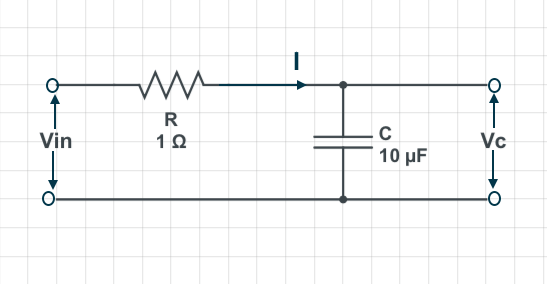
\includegraphics[width=\textwidth]{my_rc.png}
                \caption{An RC series circuit}
        \end{subfigure}
        \quad
	~
        \begin{subfigure}[b]{0.5\textwidth}
                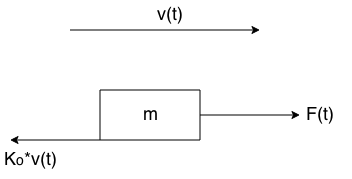
\includegraphics[width=\textwidth]{fbd.png}
                \caption{Forces acting on the mass}
        \end{subfigure}
        \caption{}
\end{figure}


\subsection{Definitions}
\subsubsection{Signal}
A signal is a ``reasonable" function of a real independent variable to the set of complex numbers in the most general case. Thus a function $x(t)$ is a signal if $x:\mathbb{R} \xrightarrow{} \mathbb{C}$ \footnote{The definition given here defines a signal with one dimensional independant and dependant variables. However signals with multidimensional independant variables are quite common as well. An image is an example with a two dimensional independant variable.} and $x(t)$ is reasonable. By reasonable, here we mean that the function should be well-behaved and hence, often something we may encounter practically. For example, the Dirichlet function $I_{Q}$ defined below is unreasonable in the sense that it is continuous nowhere on its domain and it is very improbable that this function will be encountered practically. Hence we do not consider this a signal.
\[
I_{Q}(x) =
  \begin{cases}
      \hfill 1 \hfill & \text{ if $x$ is rational} \\
      \hfill 0 \hfill & \text{ if $x$ is irrational} \\
  \end{cases}
\]

A signal is defined above to be a mapping to the set of complex numbers. The reason to consider a mapping to complex numbers is not yet clear as all the examples we have considered were real valued. However, we note that the definition given is a more general one as the set of reals is a subset of the set complex numbers. The reason for this generality will become clear as we go further in the course.\\

A couple of examples of signals are given in fig. 2 below.

%http://seismo.berkeley.edu/blog/seismoblog.php/2008/09/10/p-waves-and-s-waves-which-are-faster

\begin{figure}[H]
        \centering
        \begin{subfigure}[b]{\textwidth}
                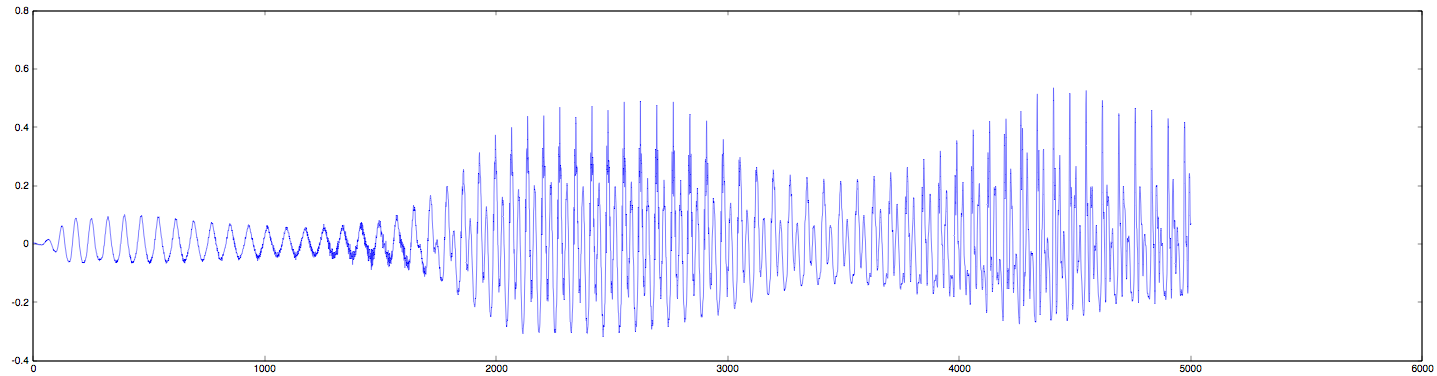
\includegraphics[width=\textwidth]{signal1_hello.png}
                \caption{An Audio Signal}
        \end{subfigure}
        \quad
        ~ %add desired spacing between images, e. g. ~, \quad, \qquad, \hfill etc.
          %(or a blank line to force the subfigure onto a new line)
        \centering
        \begin{subfigure}[b]{0.5\textwidth}
                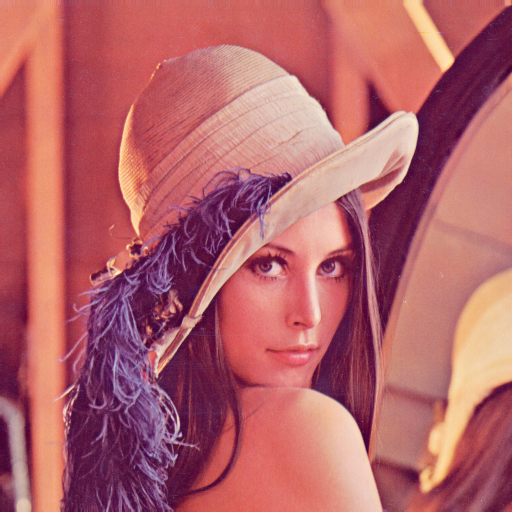
\includegraphics[width=\textwidth]{signal2_lena.png}
                \caption{An image: A 2D Signal}
        \end{subfigure}
        \caption{}
\end{figure}

\subsubsection{System}
A system is a mapping from a set of signals to another set of signals. A system thus takes a signal as an input and returns another signal as its output. A microphone is an example of a system. This system is a mapping from the set of acoustic signals to a set of electric signals.

\subsubsection{System Description}
Given a system, a system description is an explicit or an implicit relation between the inputs and the outputs of the system. By an implicit relation, we mean a relation of the form $F(x(t), y(t)) = 0$ where F is a function of two signals, the input signal $x(t)$ and the output signal $y(t)$. Thus it is not always possible to directly compute $y(t)$ directly in terms of $x(t)$. Description \textit{1} given below is an explicit system description while description \textit{2} is an implicit one.
\begin{enumerate}
\item[\textit{1}] $y(t) = x(t) + 3\frac{dx(t)}{dt}$
\item[\textit{2}] $y(t)x(t) + x(t)\frac{dy(t)}{dt} = 0$
\end{enumerate}

\subsection{Properties of Systems}
Given a system description, a lot can be inferred about the system. We describe below some properties that systems may or may not possess and give examples of each. These properties aid in the further study and classification of systems.

\subsubsection{Additivity}
A system $S$ is said to be additive if for any two input signals $x_{1}(t)$ and $x_{2}(t)$,
\[
x_{1}(t) \xrightarrow{S} y_{1}(t) \; and \; x_{2}(t) \xrightarrow{S} y_{2}(t)
\]
\begin{center}
imply
\end{center}
\[
x_{1}(t) + x_{1}(t) \xrightarrow{S} y_{1}(t) + y_{2}(t)
\]

The systems $y(t) = 3x(t)$ and $\frac{dy(t)}{dt} = x(t)$ are both additive while the system $y(t) = x(t) + 4$ (a DC shift in the case of electrical signals) is not because of the constant.

\subsubsection{Homogeneity}
A system $S$ is said to be homogenous if for every input signal $x(t)$ and for every $c \in \mathbb{C}$,
\[
x(t) \xrightarrow{S} y(t)
\]
\begin{center}
implies
\end{center}
\[
cx(t) \xrightarrow{S} cy(t)
\]

This property is also referred to as the scaling property.\\

The systems $y(t) = 3x(t)$ and $\frac{dy(t)}{dt} = x(t)$ are both homogeneous too while the system $y(t) = x(t) + 4$ is non-homogeneous again due to the presence of the non zero constant.

\subsubsection{Shift Invariance}
A system S is said to be shift invariant if for all input signals $x(t)$ and for every $t_{0} \in \mathbb{R}$,

\[
x(t) \xrightarrow{S} y(t)
\]
\begin{center}
implies
\end{center}
\[
x(t - t_{0}) \xrightarrow{S} y(t - t_{0})
\]

Intuitively, the property of shift invariance implies that if the same input is fed to the system at different times, then the output of the system will only be shifted in time by the same amount 
as that of the input.

Thus, the system $y(t) = x(t^{2})$ is shift invariant while the system $y(t) = tx(t)$ is not.\\
\textbf{Note:} The property of shift invariance is also referred to by many as time invariance.

\subsection*{Some Additional Material}
\subsubsection{Abstraction}
As the professor alludes to in the video segment, the process of abstraction is the most important tool we use for analysing and studying the natural world. A very good example of abstraction is the theory of gravitation. The insight that an apple falling from the tree (and supposedly hitting his head) and the Moon revolving around the Earth are actually the same thing was something only Newton could have had. In his words, ``....I began to think of gravity extending to the orb of the Moon....''. At that moment in history, he abstracted out all the differences between the moon and the apple to come up with the theory of universal gravitation. The word universal in the name is important as it states how we can think of (i.e abstract) every mass in the Universe as a point mass attracting every other. That is the power of abstraction as the instructor stresses in the video segment.

However one must keep in mind that the real art lies in finding the right kind and the right level of abstraction for the specific kind of job at hand. Suppose a chemist wants to study chemical behaviour of ethanol and methanol in connection with their reactions with some particular chemical. In that case, abstracting out the fact whether it is methyl or ethyl alcohol and studying, in generality the reactions of the alcohol part of the two (i.e. of the -OH group) with the desired chemical considerably reduces the work of the chemist. However, we cannot use the same abstraction when studying the biological effects of the two as methanol is highly toxic and can be fatal in sufficient quantities; however ethanol is not toxic and is used for....well we all know!



\section{Module 1: Lecture 4\\ System Properties: An Illustration}


\subsection{Introduction}
Recall the definitions of additivity, homegeneity and shift-invariance. In the last lecture, we saw that a system with the description, $y(t) = x(t) + 5$ is neither additive nor homogeneous. Is it shift-invariant? It is because applying the definition of shift-invariance, it can be seen that $y(t - t_{0}) = x(t - t_{0}) + 5$. In this lecture, we will consider a real-life example of a system and apply the definitions to analyse its additivity, homogeneity and shift-invariance. 

\subsection{RC Circuit}

\begin{center}
\begin{circuitikz} \draw;
begin{circuitikz}[scale=2];
    \def\xPortLeft{0}
    \def\yTerminalBottom{0}
    \def\yL{1.5}
    \def\xR{1.75}
    \def\xC{2.25}
    \def\xPortRight{3}
    % left loop
    \draw                               (\xPortLeft,\yL)
            to[R=$R$, o-]               (\xR, \yL)
            to[short]                   (\xC,\yL)
            to[C, l_=$C$,*-*]           (\xC,\yTerminalBottom)
            to[short]                   (\xPortLeft,\yTerminalBottom)
            to[voltmeter,v^>=$x(t)$,o-o]   (\xPortLeft,\yL);
    % right branch
    \draw                               (\xC,\yL)
            to[short]                   (\xPortRight,\yL)
            to[open,v^=$y(t)$,o-o]    (\xPortRight,\yTerminalBottom)
            to[short]                   (\xC,\yTerminalBottom);
\end{circuitikz}
\end{center}


Let us derive the system description for this RC circuit. Applying Kirchoff's Voltage law, we get $x(t) - i(t)R - y(t) = 0$ where $i(t) = C\frac{dy(t)}{dt}$. So we get,
\begin{equation}
x(t) = RC\frac{dy(t)}{dt} + y(t) \nonumber
\end{equation}

There is a way to check whether both additivity and homogeneity are simulatenously satisfied, using the test of \textit{superposition}.
A system is said to obey the principle of superposition if any \textit{linear combination of the inputs gives the same linear combination of the outputs}. Consider two different inputs $x_{1}(t)$ and $x_{2}(t)$, giving outputs $y_{1}(t)$ and $y_{2}(t)$ respectively. We ask whether, $\alpha x_{1}(t) + \beta x_{2}(t)$ yields $\alpha y_{1}(t) + \beta y_{2}(t)$ {\bf for all} possible $x_{1}, x_{2}, \alpha$ and $\beta$? If so, the system obeys superposition and hence is both additive and homogeneous. Let us apply it to the RC circuit system. 
\begin{equation}\label{eq:RC1}
x_{1}(t) = RC\frac{dy_{1}(t)}{dt} + y_{1}(t)
\end{equation}
\begin{equation}\label{eq:RC2}
x_{2}(t) = RC\frac{dy_{2}(t)}{dt} + y_{2}(t) 
\end{equation}
Multiplying \eqref{eq:RC1} by $\alpha$ and \eqref{eq:RC2} by $\beta$ and adding, we get
\begin{equation}
\begin{split}
\alpha x_{1}(t) + \beta x_{2}(t) & = RC\frac{d\alpha y_{1}(t)}{dt} + \alpha y_{1}(t) + RC\frac{d\beta y_{2}(t)}{dt} + \beta y_{2}(t) \\
& = RC\frac{d (\alpha y_{1}(t) + \beta y_{2}(t))}{dt} + (\alpha y_{1}(t) + \beta y_{2}(t))
\end{split}
\end{equation}
Since $x_{1}, x_{2}, \alpha$ and $\beta$ are arbitrary, it holds for all possible values of these. Therefore, the RC system obeys principle of superpostion. 
\\

The physical interpretation of superposition is that inputs are scaled and then added one on top of the other, or in other words \textit{superposed}. If the outputs also undergo the same scaling and addition, {\bf for all} possible scaling factors and inputs, the system obeys the principle of superposition.The principle of superposition subsumes additivity and homogeneity. That is, if the principle of superposition holds, additivity and homogeneity will both hold.

\subsubsection*{Additivity} In the principle of superposition, substitute $\alpha$ and $\beta$ both equal to 1. We get back the property of additivity. Does $x_{1}(t) + x_{2}(t)$ yield $y_{1}(t) + y_{2}(t)$ for all possible $x_{1}$ and $x_{2}$?

\subsubsection*{Homogeneity} In the principle of superposition, substitute $\beta = 0$. We get back the property of homogeneity. Does $\alpha x_{1}(t)$ yield $\alpha y_{1}(t)$ for all possible $x_{1}$ and $\alpha$?
\\

Now that it is proved that the system is superposable, let us ask the question - \textit {What changes can we make to the properties of the RC circuit system to destroy its superposability?}

\subsection{Introduction}
Recall the definitions of additivity, homegeneity and shift-invariance. In the last lecture, we saw that the RC circuit system obeys the principle of superposition. That is, it is both additive and homogeneous. In this lecture, we will see how this can be destroyed by small changes and also analyse its shift-invariance property. 

\subsection{RC Circuit}
We first start with the question : \textit {What changes can we make to the properties of the RC circuit system to destroy its superposability?} One possibility is to introduce a little nonlinearity to the system by making the response of the resistor different.
\\

For example, instead of $V \propto i$, we could have $V \propto i^{\gamma}$. This is quite true since real resistances do have a nonlinear regime. In microelectronics, resistances are made of semiconductor devices which do not have the ideal Ohm's law behaviour. Let us consider what would happen to the system in this case. Using the Kirchoff's voltage law like last time, the system description can be derived to be 
\begin{equation}
x(t) = R({C\frac{dy(t)}{dt}})^{\gamma} + y(t) \nonumber
\end{equation}
It is left as an exercise for the reader to show that this system no longer obeys superposition. This implies that the system is not \textit{both} additive and homogeneous. One must also show that the system is \textit{neither} additive nor homogeneous. 
This question has been raised to point to the fact that all real systems behave linearly over a regime and not always. 
\\

\begin{center}
	\begin{circuitikz} \draw;
		begin{circuitikz}[scale=2]
		\def\xPortLeft{0}
		\def\yTerminalBottom{0}
		\def\yL{2.0}
		\def\xR{1.75}
		\def\xC{2.25}
		\def \Vc{3.0}
		\def\xPortRight{4.0}
		\def \Vol{1.0}
		% left loop
		\draw                               (\xPortLeft,\yL)
		to[R=$R$, o-]               (\xR, \yL)
		to[short]                   (\xC,\yL)
		to[C, l_=$C$,*-]              (\xC,\Vol)
		to[battery1, v^=$2$V, -*]   (\xC, \yTerminalBottom)
		to[short]                   (\xPortLeft,\yTerminalBottom)
		to[voltmeter,v^>=$x(t)$,o-o]   (\xPortLeft,\yL);
		% right branch
		\draw                               (\xC,\yL)
		to[short]                   (\xPortRight,\yL)
		to[open,v^=$y(t)$,o-o]      (\xPortRight,\yTerminalBottom)
		to[short]                   (\xC,\yTerminalBottom);
		
		\draw                               (\xC, \yL)
		to[short]                   (\Vc,\yL)
		to[open,v^=$V_{c}(t)$,-*]      (\Vc,\Vol)
		to[short]                   (\xC,\Vol);
		
	\end{circuitikz}
\end{center}
Another way in which superposition can be destroyed is by adding a \textit{DC offset}. This can be introduced by adding a DC voltage source in series with the capacitor. Earlier, we had the capacitor voltage $V_{c}(t) = y(t)$. Now, we have $V_{c}(t) + 2 = y(t)$. The system description can be written using Kirchoff's voltage law. $x(t) - i(t)R - V_{c}(t) - 2 = 0$, where $i(t) = C\frac{dV_{c}(t)}{dt}$. So we get,
\begin{equation} \label{eq:nl}
x(t)  = RC\frac{dV_{c}(t)}{dt} + V_{c}(t) + 2 
\end{equation}
\begin{equation} \label{eq:l}
x(t) = R{C\frac{dy(t)}{dt}} + y(t) 
\end{equation}
This is the same as before and so it obeys principle of superposition. Now, if we were to consider the output to be $V_{c}(t)$ and not $y(t)$, the system description would be \eqref{eq:nl}. This is similar to the system description $y(t) = x(t) + 5$. Using the same technique as before, the reader has to show that the system described by \eqref{eq:nl} is neither additive nor homogeneous. 

\subsubsection*{Shift-invariance}
Is the system described by \eqref{eq:l} is shift-invariant? In other words, is it true that
\begin{equation}
x(t-t_{0}) = RC\frac{dy(t-t_{0})}{dt}+ y(t-t_{0}) ? \nonumber
\end{equation}
Yes. This is because the derivative operator is shift-invariant since $\frac{dy(t - t_{0})}{dt} \equiv \frac{dy({\lambda})}{d\lambda}$, where $\lambda = t - t_{0}$. 
\\

Question: Is the system described by \eqref{eq:nl} shift-invariant?








\section{Module 1: Lecture 5\\ Challenging Problems}


\subsection{Introduction}
So far, we have looked at systems which are either both additive and homogeneous or neither additive nor homogeneous. But they are independent properties. In this lecture, we shall look at examples of \textit{complex-valued} systems which are additive but not homogenous and vice versa. 

\subsection{Two systems}
\textit{Complex-valued} systems are those whose inputs and outputs are complex functions of time. That is, $x(t)$ and $y(t)$ take values belonging to $\mathbb{C}$ (the set of complex numbers). 
\\

{\bf System 1 :}
\begin{equation}
y(t) = \operatorname{Re}(x(t)) \nonumber
\end{equation} 
Is this system additive? Is it homogeneous? (Remember that the constant $\alpha$ can be complex)? Is it shift-invariant? 
\\

{\bf System 2 :}
\[
    y(t)= 
\begin{cases}
    \frac{x(t)x(t-1)}{x(t-2)},& \text{if } x(t-2) \neq 0\\
    0,              & \text{otherwise}
\end{cases}
\]
Is this system additive? Is it homogeneous? Is it shift-invariant? 
\\

The systems are, in fact, shift-invariant as shifting the input by any constant $t_{0}$ in time, will result the output to also shift by the same amount in time. What can we do to the system to make them \textit{shift-variant}? Note that shift-invariance can be destroyed by having a time-dependancy in the system description. Here is an example of explicit time-dependence. 
\begin{equation}
y(t) = tx(t) \nonumber
\end{equation} When the input is shifted by $t_{0}$, we get the output to be $tx(t-t_{0})$ which is not equal to $y(t-t_{0}) = (t-t_{0})x(t - t_{0})$. 
\\

Systems with the three properties of additivity, homogeneity and shift-invariance are very important because (a) they are easy to analyse and (b) they are easy to realise. Any electrical system consisting of ideal resistors, capacitors and inductors obeys these three properties. Mechanical systems consisting of springs and masses obey these three properties. For example, a hydraulic system can be modeled as the RC circuit that we previously saw. A tank which stores water is analogous to a capacitor which stores charge; a pipe which allows water to flow between its two ends is analogous to a resistor which allows current to pass through it. 

{\bf Challenge} : Build a system description of a tank analogous to the capacitor using basic fluid equations. 
\textit{Hint} - Let the pressure difference between the top and bottom of the tank $P_{0}(t)$ be the output and the height of water in the tank $h(t)$ be the input. The derivative relation arises from the speed of water $v_{1}(t)$ and the instantaneous height $h(t)$ as $v_{1}(t) = \frac{dh(t)}{dt}$.
\\

{\bf Challenge} : Build a system description of a pipe analogous to the resistor using basic fluid equations.
\textit{Hint} - Let the pressure difference across the pipe $P_{a}(t) - P_{b}(t)$ be the output and the velocity of the fluid through the pipe $v_{2}(t)$ be the input. There is a linear relationship between the two.
\\

{\bf Challenge} : By attaching the pipe to the bottom of the tank, build a system description of the tank and pipe system analogous to the resistor-capacitor system.\newline\textit{Hint} - Let the input be the difference in the pressures between the top of the tank to the free end of the pipe. Let the output be the pressure difference across the tank. 












\section{Module 1: Lecture 6\\ Impulse Response: A Building Block for Continuous Functions}

	

\subsection{Introduction}
As mentioned in the previous lecture, systems which obey the three properties of additivity, homogeneity and shift-invariance are desirable since they are easy to analyse and build. In this lecture, we will make a start to understand why this is so, by introducing the concept of narrow pulses. 

\subsection{Narrow pulses}
Narrow pulses can be used to construct \textit{reasonable signals}. Reasonable signals or smooth signals are those which do not have infinite number of discontinuites in a finite interval. Therefore, there exists an interval where the signal is continuous. Consider the signal over such an interval. 
\\

%add diagram here
Divide the interval into sub-intervals of size as small as can be. Consider one such sub-interval. As the width of this sub-interval grows smaller and smaller, the value that the signal takes over it does not change much and is almost a constant. 
%add diagram of pulse of width \Delta here
\\

Consider a narrow pulse of width $\Delta$. Let its height be $\frac{1}{\Delta}$, such that its area is unity. This is our basic building block. When this pulse is placed a point in time $t$ and multiplied by the signal, we get a pulse of height \textit{proportional} to the (constant) value of the signal in that interval (the proportionality factor being  $\frac{1}{\Delta}$). 

Now copy and shift the initial pulse (of width $\Delta$ and height $\frac{1}{\Delta}$) in the time-axis in steps of $\Delta$ so as to cover the entire time-axis. Multiply it by the signal and combine all of it together. We get back something very similar to the original signal. Smaller the pulse width, more the similarity to the original signal. 
%add diagram here

\subsection{Sifting property}
Let $x(t)$ be the continuous function. Reconsider the narrow pulse that we constructed in the previous lecture, placed at $t = 0$. It has width $\Delta$ and height $\frac{1}{\Delta}$. This can be called as {\bf $\delta_{\Delta}(t)$}. %add figure here!! 
\\

Place one such pulse (red) at $t = t_{0}$ on the time-axis as shown in figure ..It is $\delta_{\Delta}(t - t_{0})$. Multiply $x(t)$ with $\delta_{\Delta}(t - t_{0})$ and integrate over all time $t$. That is,
\begin{equation} \label{int}
\int_{-\infty}^\infty x(t) \delta_{\Delta}(t - t_{0}) dt 
\end{equation}
If $\Delta $ is small enough, the function over the non-zero part of the pulse is almost a constant which can be taken to be $x(t_{0})$. So the above integration simply picks out the value of the function at one point $t_{0}$. This can be seen in the following.
\begin{equation}
x(t) \delta_{\Delta}(t - t_{0}) \equiv x(t_{0}) \delta_{\Delta}(t - t_{0})
\end{equation} 
This is true because the product of the function and the narrow pulse is zero everywhere except over the small interval around $t_{0}$, where the function is almost a constant. Now keeping in mind that the area of $\delta_{\Delta}(t)$ pulse is unity, if we were to perform the integration as \eqref{int}, we would get,
\begin{equation}
\begin{split}
\int_{-\infty}^\infty x(t) \delta_{\Delta}(t - t_{0}) dt  & = \int_{-\infty}^\infty x(t_{0}) \delta_{\Delta}(t - t_{0}) dt \\
& = x(t_{0})  \int_{-\infty}^\infty \delta_{\Delta}(t - t_{0}) dt \\
& = x(t_{0})
\end{split}
\end{equation} 
So the $\delta_{\Delta}(t - t_{0})$ pulse is like a sieve which sifts or picks out the value of the function at $t_{0}$. 

\subsection{Stitching together a function with narrow pulses}
We can derive a different interpretation of this integration property. Construct the $\delta_{\Delta}(t)$ pulse to be symmetric about the $t$-axis such that $\delta_{\Delta}(-t) = \delta_{\Delta}(t)$.  %add figure here!!
Since, 
\begin{equation} \label{sift}
\int_{-\infty}^\infty x(t) \delta_{\Delta}(t - t_{0}) dt = x(t_{0})
\end{equation}
it is true that, 
\begin{equation} \label{const}
\int_{-\infty}^\infty x(t) \delta_{\Delta}( t_{0} - t) dt = x(t_{0})
\end{equation}
The meanings of the equations \eqref{sift} and \eqref{const} are very different. \eqref{sift} says that multiplying a function by the narrow pulse and integrating over all time results in pulling out the value of the function at the point at which the pulse is located.
\\

For interpreting the meaning of \eqref{const}, consider $t_{0}$ to be the basic variable by which the function is indexed/described. Take any point t and multiply the value of the function at that point $x(t)$ with the narrow pulse at that point. Then take a sum over all such $t$. This sum tends to an integral in the limit. This integral which is the limit of this sum is precisely given by \eqref{const}. It can be thought of as,
\begin{equation}
x(t_{1})\delta_{\Delta}(t_{0} - t_{1}) + x(t_{2})\delta_{\Delta}(t_{0} - t_{2}) + x(t_{3})\delta_{\Delta}(t_{0} - t_{3}) + ...
\end{equation}
Graphically, it means, %attach figure here!!
Put a narrow pulse at every possible $t_{0}$ and multiply with the function value at that point. So each pulse will have a height $=$ \textit({value of the function at that point}) ($\frac{1}{\Delta}$). As there is a continuum of pulses, combining the pulses leads to the integral whose value is nothing but the function itself, in the limit $\Delta \rightarrow 0$. This gives the interpretation that 
{\bf Every function is a combination of an infinite number of very narrow pulses}.
\\

Note that these narrow pulses are such that even as $\Delta$ goes to zero, the height grows as $\frac{1}{\Delta}$, keeping the area always equal to unity. 
\section{Lecture 7. Impulse Response and Properties of Systems}


\subsection{The Continuous Variable Delta Function}
We defined the continuous time delta function as a function which assumes the value 0 everywhere except in an interval $\Delta$ around the origin, where it assumes the value $\frac{1}{\Delta}$, and then we take the limit as $\Delta \rightarrow 0$. Refer to fig. 1. \\ 
\begin{figure}[H]
	\centering
	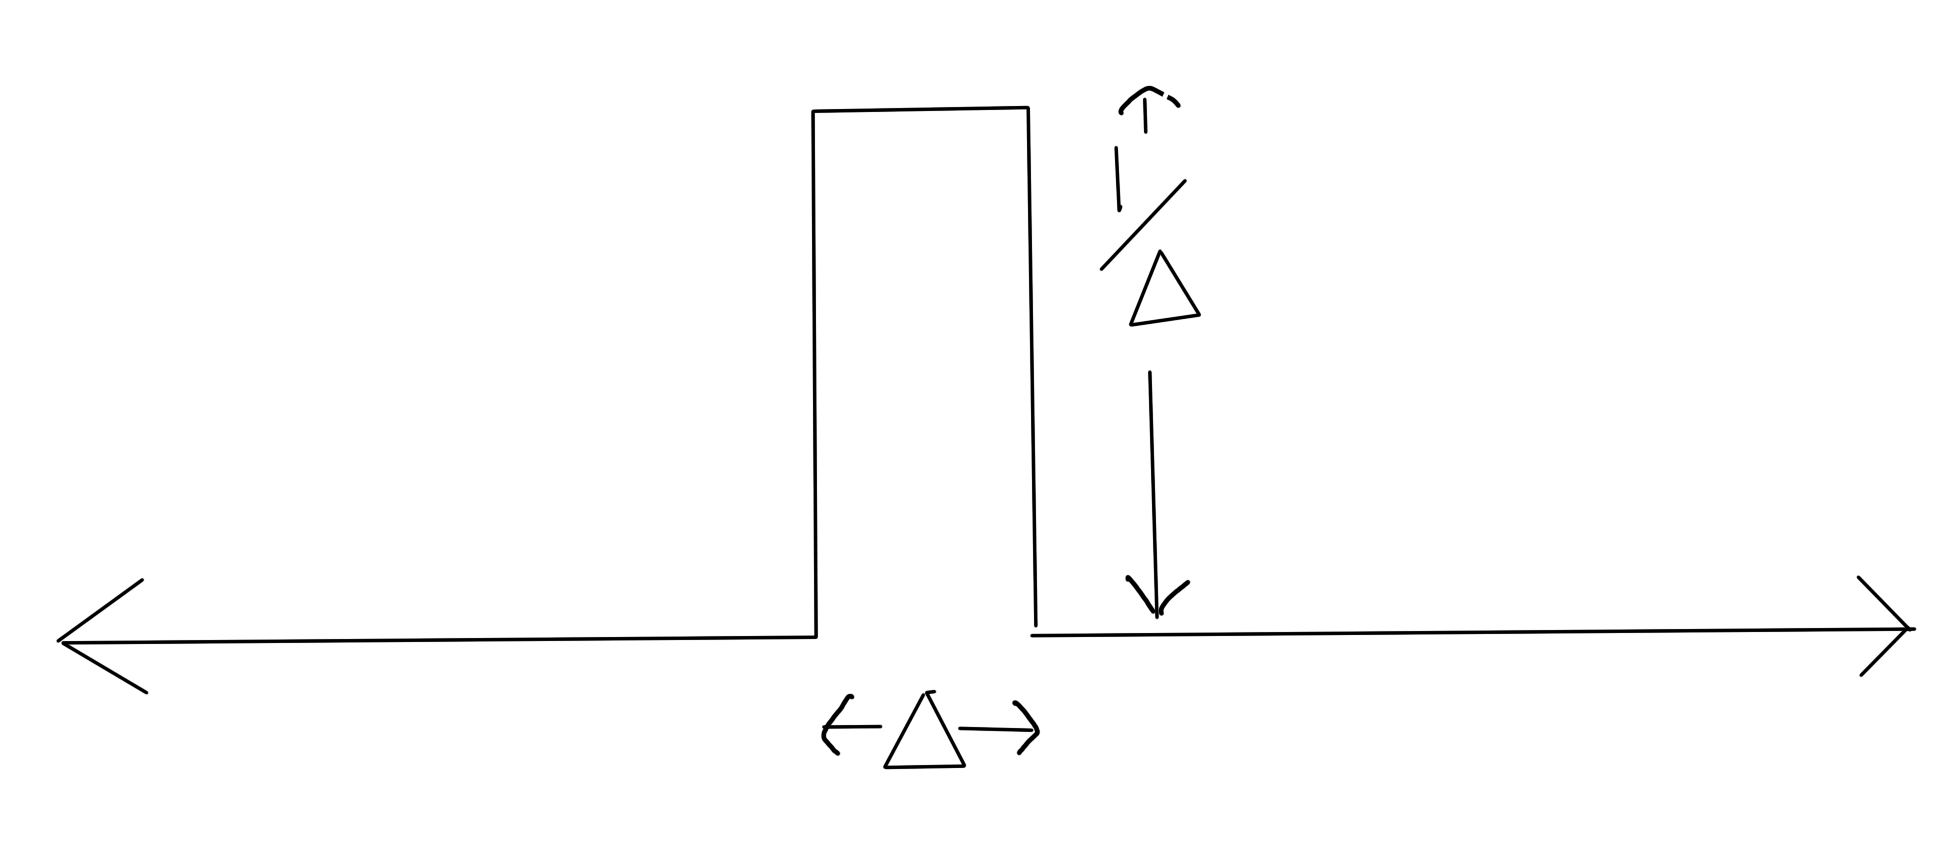
\includegraphics[width=0.5\textwidth]{delta1.png}
	\caption{The $\delta_\Delta$ function, centred at the origin}
\end{figure}
Thus, the area under the function, i.e. the integral of the function from $-\infty$ to $+\infty$ is unity, while the function is zero at all points except the origin.\\
\indent It should be noted that the delta function is not a function in the conventional sense. This is because, the delta function does not have a well-defined value at the origin. We call the delta function a ``generalized function". Generalized functions are generalizations or extensions of the concept of a function, but are not really functions.\\
\indent We will also refer to the delta function as a ``unit impulse". The unit impulse captures an area of unity while having zero width. The conventional way of representing a unit impulse is shown in fig. 2.\\
\begin{figure}[H]
	\centering
	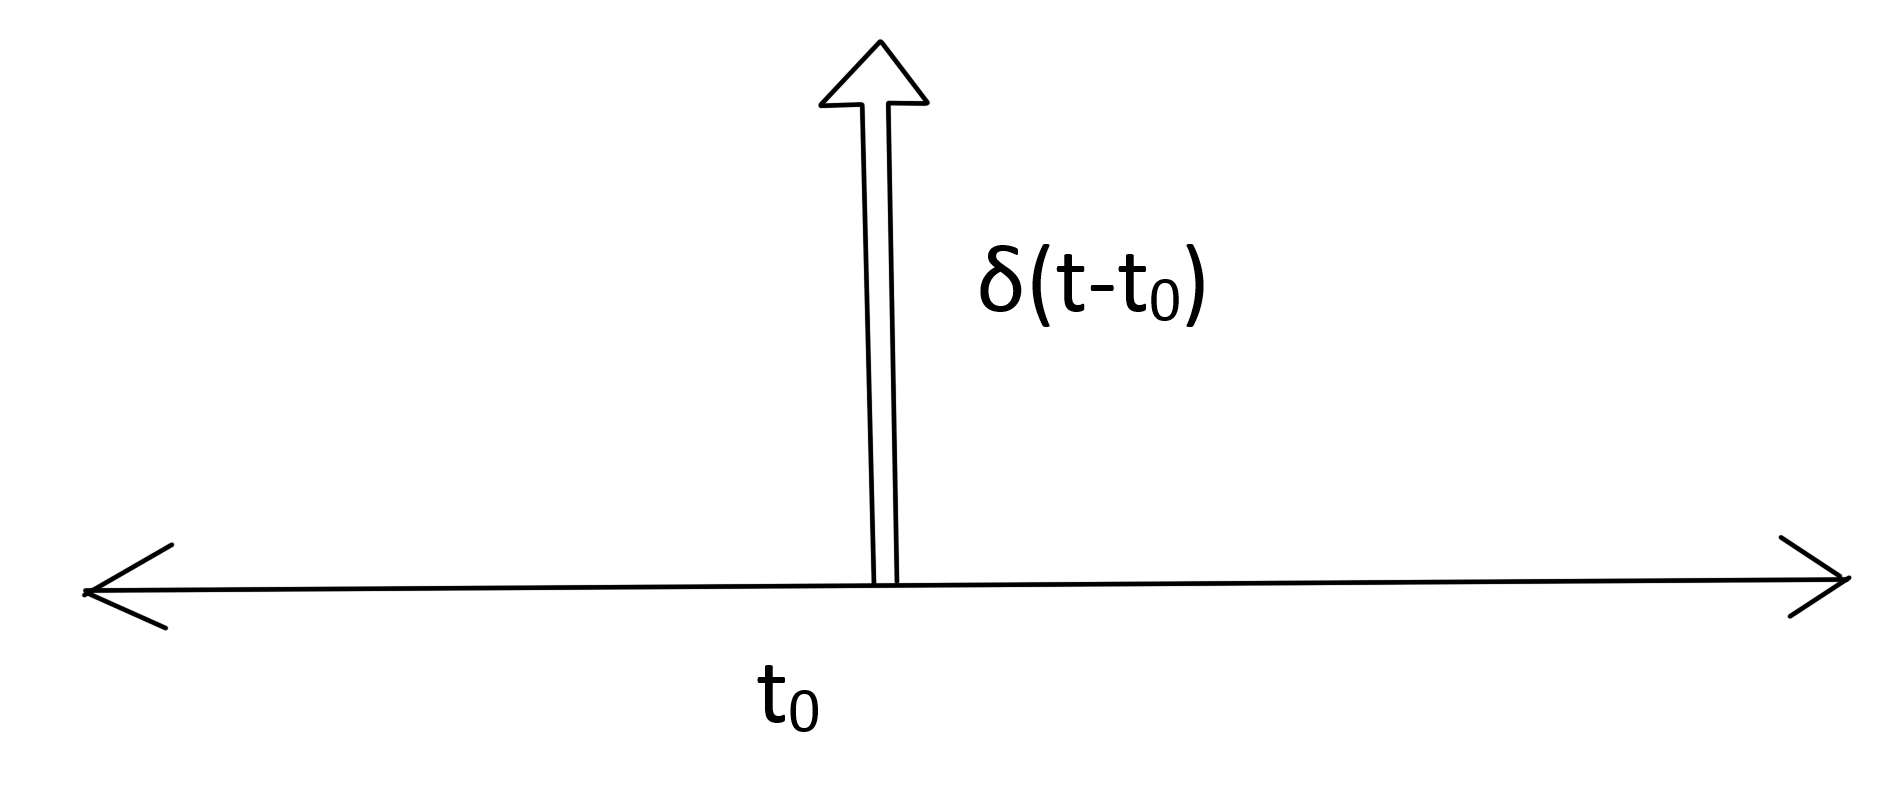
\includegraphics[width=0.5\textwidth]{delta2.png}
	\caption{Representing the unit impulse graphically}
\end{figure}
\indent Now, if we use the symbol $\delta_\Delta (t)$ for the above mentioned function with finite $\Delta$, then in accordance with the definition above,
$$\lim_{\Delta\rightarrow 0}\delta_\Delta(t)=\delta(t)$$
Where, we denote by $\delta(t)$ the unit impulse function.
%\subsection{Using unit impulse to get the value of a function at a particular point}
%We can get back the value of a function at a particular point if we integrate the delta function weighted properly, as is in the following equation:
%$$x(t_0)=\int_{-\infty}^{\infty	} x(t)\delta(t_0-t)dt$$
%\indent Thus, the delta function centred at a particular point multiplied by a function, gives the value of the function at that point when integrated over the entire real axis.

\subsection{Unit Impulse Response}
Assume that we give to a system, a unit impulse/delta function as its input. The output that is obtained is called the impulse response of that system. \\
\indent Although practically, we cannot generate an impulse function, one can imagine giving to the system $\delta_\Delta$ functions as inputs, successively, with decreasing values of $\Delta$ and obtain a good estimate of the Unit Impulse Response.\\
\indent Thus, in short, \textbf{the impulse response is the output of a system, when the input is a unit impulse.} (Fig. 3)
\begin{figure}[H]
	\centering
	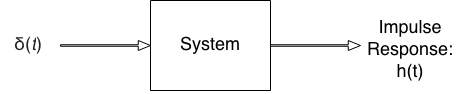
\includegraphics[width=0.5\textwidth]{Block-impulseresponse.png}
	\caption{Unit Impulse Response}
\end{figure}

\subsubsection{Impulse response of an LSI system}
Consider a linear shift-invariant system \textbf{S}. Now, suppose that we give as the input, the sum of two unit impulses centred at two different points $t_1$ and $t_2$. Due to additivity, we expect the output to be the sums of the corresponding outputs. (fig. 4(a))\\
\indent Also, because of homogeneity, we expect that the output corresponding to the input $\kappa\delta(t)$ should be $\kappa h(t)$ where h(t) is the unit impulse response and $\kappa\in\mathbb{C}$ (fig. 4(b))
\begin{figure}[H]
        \centering
        \begin{subfigure}[b]{0.8\textwidth}
                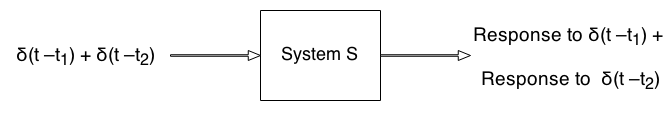
\includegraphics[width=\textwidth]{Block-additivityimpulseresponse1}
                \caption{Consequence of Additivity of \textbf{S}}
        \end{subfigure}
        \quad
	~	\quad
        \begin{subfigure}[b]{0.6\textwidth}
                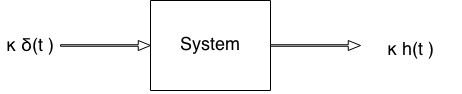
\includegraphics[width=\textwidth]{block-homogeneity}
                \caption{Consequence of Homogeneity of \textbf{S}}
        \end{subfigure}
        \caption{}
\end{figure}

Now, if we took $\kappa$ to be the value of a function $x$ at some point, then the property still holds.\\
\indent Let us not consider the output of $\delta(t-t_0)$, which is nothing but $\delta(t)$ shifted to the right by $t_0$ units. Thus, due to shift invariance, we expect that the output to $\delta(t-t_0)$ should be $h(t-t_0)$.(fig. 5)

\begin{figure}[H]
	\centering
	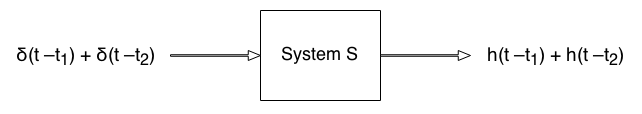
\includegraphics[width=0.7\textwidth]{Block-shiftinv.png}
	\caption{Consequence of shift-invariance of \textbf{S}}
\end{figure}

Now assume that we have points $\lambda_1$, $\lambda_2$ and $\lambda_3$. As a consequence of Homogeneity, Additivity and Shift-Invariance of \textbf{S}, we know that the output corresponding to $x(\lambda_1)\delta(t-\lambda_1)+x(\lambda_2)\delta(t-\lambda_2)+x(\lambda_3)\delta(t-\lambda_3)$ will be $x(\lambda_1)h(t-\lambda_1)+x(\lambda_2)h(t-\lambda_2)+x(\lambda_3)h(t-\lambda_3)$.\\
\indent We can think of an integral as a summation of many such products $x(\lambda)\delta(t-\lambda)$ where the $\lambda$'s are brought infinitesimally close to each other. Thus, we can consider the integration as a summation over a continuum of $\lambda$'s. (fig. 6)

\begin{figure}[H]
	\centering
	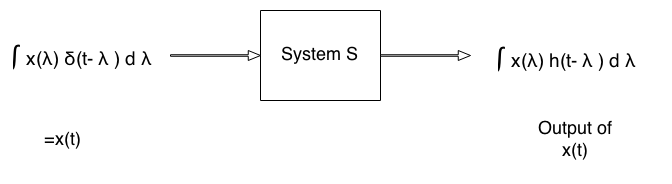
\includegraphics[width=0.8\textwidth]{Block-characterization1.png}
	\caption{Consequence of Linear shift-invariance of \textbf{S}}
\end{figure}
\indent As discussed in the previous lecture, the input integral equates to $x(t)$. Thus, we have obtained a way of obtaining the output corresponding to any signal $x(t)$ using the impulse response.\\\\
\noindent\fbox{%
    \parbox{\textwidth}{%
       \textbf{Given the impulse response of an Linear Shift-Invariant System, we can calculate the output corresponding to any input signal.}
    }%
}
\\\\
This is a very important result in signals and systems, because knowing the output of just one function gives us the power to know beforehand, what the output should be for any input provided to the LSI system.

\section{Lecture 8: Relating Unit Step and Unit Impulse}


\subsection{Impulse Response of for an RC circuit}
In the discussion about the importance of abstraction, we had come across two systems, the RC circuit, and the mass-force system, which had the same behaviour. Now, since the RC circuit system is a Linear Shift-Invariant system, it would be useful to acquire its unit impulse response, since this will empower us to obtain the output signal, for any given input signal.\\
\indent Recall that for the RC circuit system, we took the voltage applied across the resistor and the capacitor to be the input voltage ($V_{in}$ - the input signal), while the voltage across the capacitor to be the output voltage ($V_C$ - the output signal). (fig. 1)
\begin{figure}[H]
	\centering
	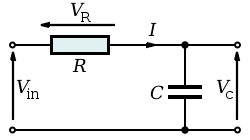
\includegraphics[width=0.4\textwidth]{./rc.png}
	\caption{RC circuit diagram}
\end{figure}
\indent Now, we had defined the unit impulse as a limiting case of the $\delta_\Delta$ function, whose width was $\Delta$, and whose area under the curve was unity.\\
\indent To find the unit impulse response, we need to go back to the differential equation governing the RC circuit. We know that the current in the circuit is proportional to the derivative of the capacitor voltage. i.e.
$$I=C\frac{dV_C}{dt}$$
\indent On integrating both the sides w.r.t. t, we get 
$$\int I dt = CV_C$$
\indent Instead of dealing with the Voltage directly, we will look at the integrated form. Thus arises the question: What is the integral of the unit impulse?
\subsubsection{Integral of the unit impulse}
Consider the $\delta_\Delta$ function centred at $t_0$. Now consider the running integral:
$$\textrm{Running Integral of }\delta_{\Delta,t_0} = \int_{-\infty}^t \delta_{\Delta,t_0}(\lambda)d\lambda$$
\indent Let us now divide the $\delta_{\Delta,t_0}$ function into three regions(fig. 2(a)):
\begin{itemize}
\item Region 1: The region $t<t_0$
\item Region 2: The region where $t_0< t <t_0+\Delta$
\item Region 3: The region $t>t_0+\Delta$
\end{itemize}
\indent We can see that the integral in Region 1 is zero since $\delta_{\Delta,t_0}$ is $0$ and that the only region where we need to calculate the integral is Region 2.\\
\indent The integral of a constant function is a linear function, and since we know that the area under the $\delta_\Delta$ function is unity, it is clear that the running integral increases linearly from 0 at $t=t_0$ to 1 at $t=t_0+\Delta$ after which, it remains 1 in Region 3. (fig. 2(b))
\begin{figure}[H]
        \centering
        \begin{subfigure}[b]{0.5\textwidth}
                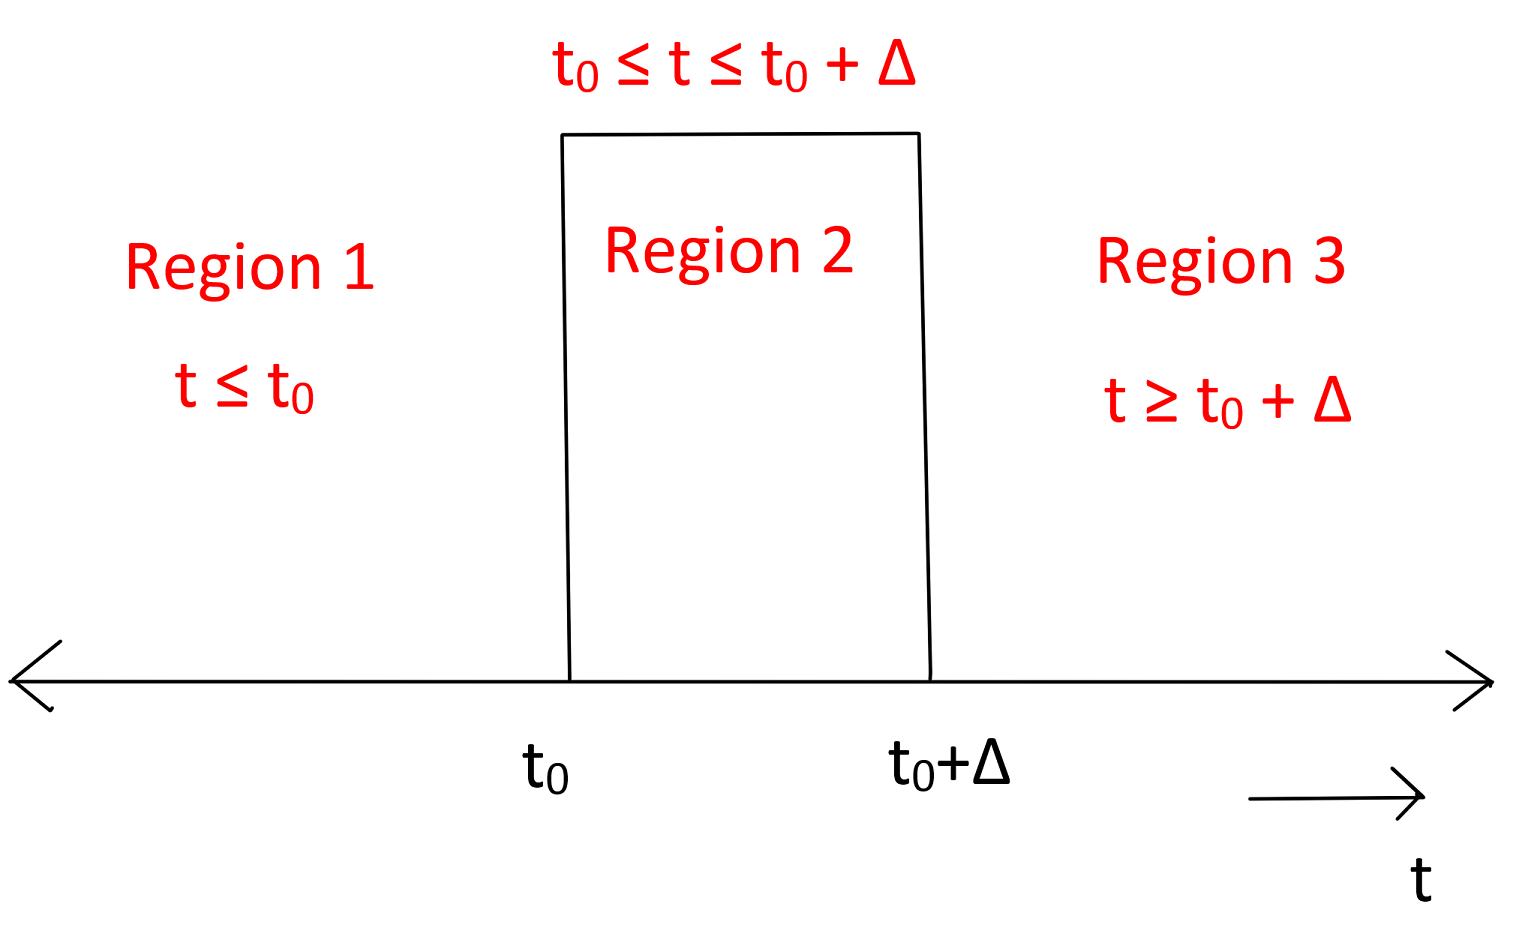
\includegraphics[width=\textwidth]{./regions_of_delta.png}
                \caption{Dividing the $\delta_\Delta$ function into 3 regions}
        \end{subfigure}
        \quad
	~	\quad
        \begin{subfigure}[b]{0.5\textwidth}
                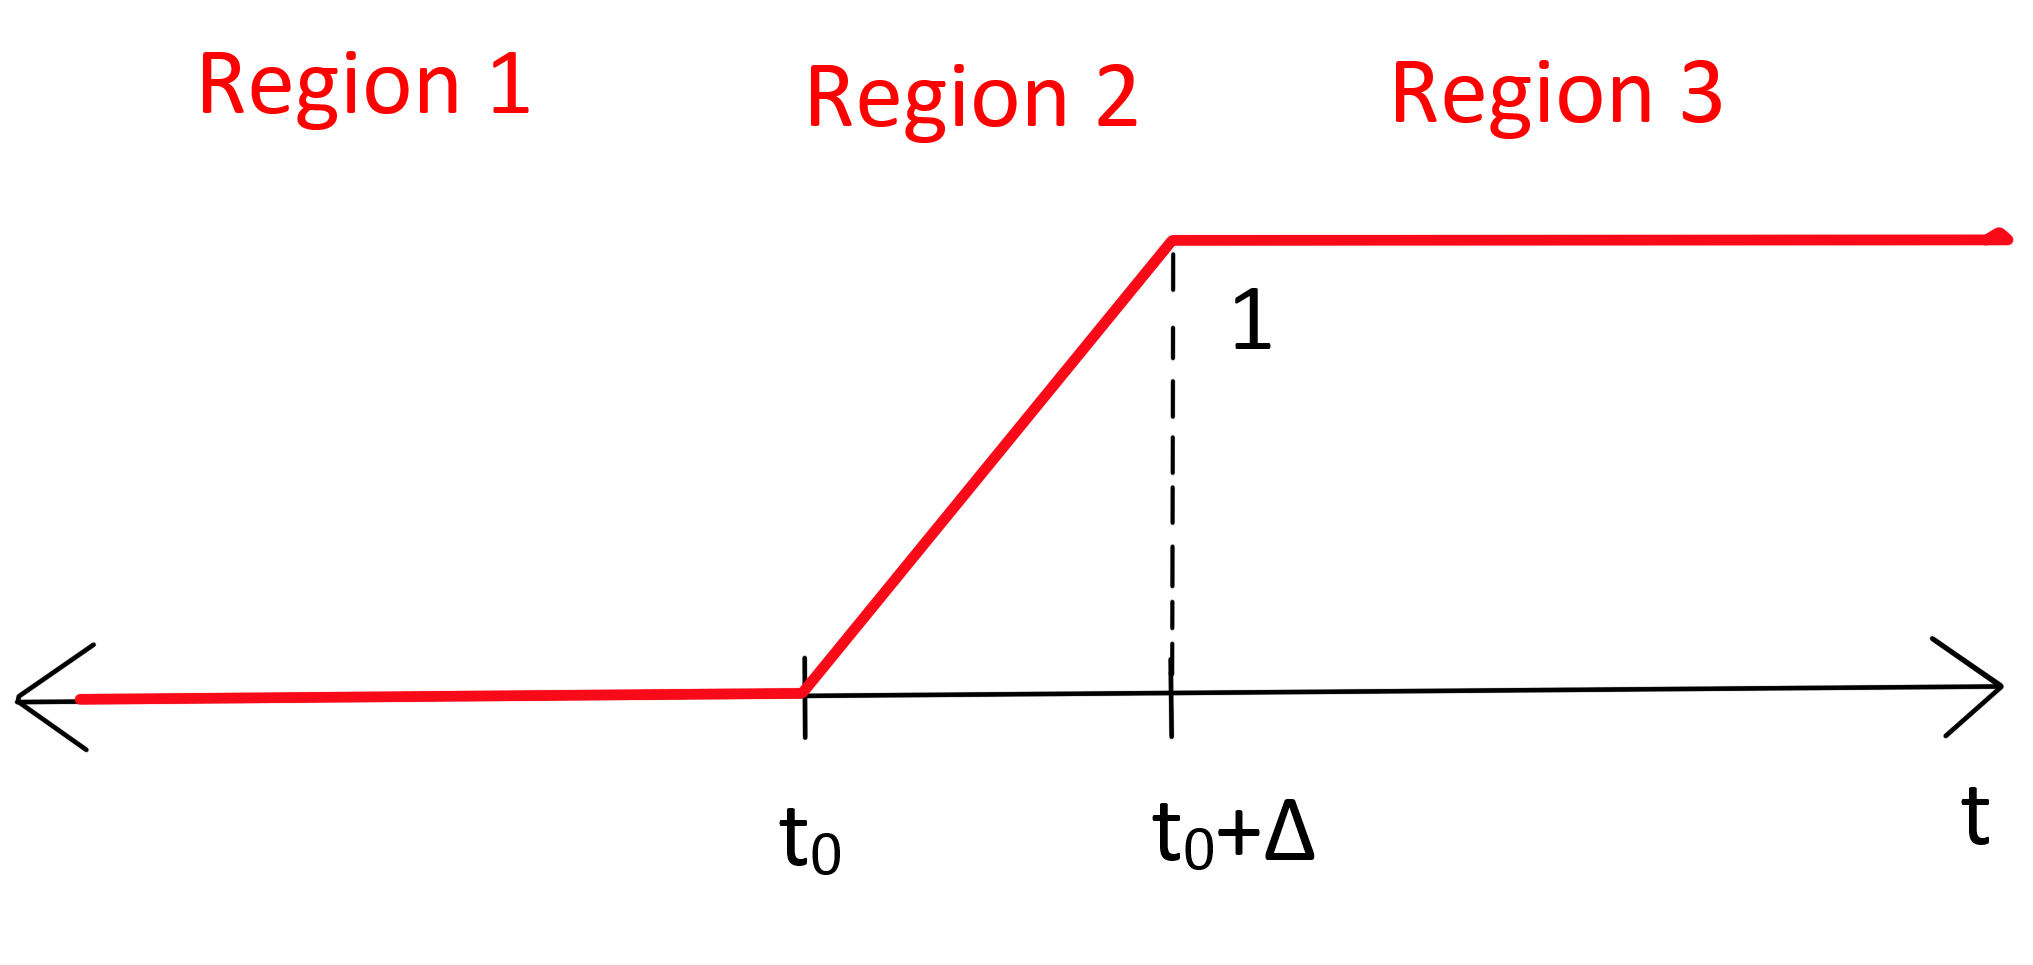
\includegraphics[width=\textwidth]{./running_integral_of_delta.png}
                \caption{Running integral of delta function}
        \end{subfigure}
        \caption{}
\end{figure}
\indent Now, to find the unit impulse response, we need to let $\Delta\rightarrow 0$. Clearly, Region 2 vanishes and we get the unit step, located at $t_0$.
Thus, 
\\\\
\noindent\fbox{%
    \parbox{\textwidth}{%
       \textbf{The running integral of the unit impulse is the unit step function, and the derivative of the unit step function is the unit impulse}
    }%
}\footnote{Note that in the classical sense of the derivative, it is not possible to take the derivative of the unit step at the origin, since it is a discontinuous function. Just as the unit impulse is not really a function, but a generalized function, the derivative of the unit step function is not a usual derivative, but is a `generalized derivative'. However, without going in the subtleties of the definition of a generalized derivative, we shall move ahead without distinguishing between the classical and generalized derivatives}
 
$$\textrm{Unit Impulse}\xrightarrow {\textrm{running integral}} \textrm{Unit Step}$$
$$\textrm{Unit Impulse}\xleftarrow {\textrm{derivative}} \textrm{Unit Step}$$
\indent Now, the derivative of a function $x(t)$ is defined as:
$$\frac{dx(t)}{dt}=\lim_{\Delta\rightarrow 0}\frac{x(t+\Delta)-x(t)}{\Delta}$$
\indent	The term $x(t+\Delta)$ can be considered as the function $x(t)$ shifted to the left by $\Delta$ units. Thus, the derivative can be thought of as the difference of the original function and a shifted version of the same function, divided by the shift in the limit of the shift going to zero. This is a more `Signals and Systems' way of thinking of derivatives of signals. The original aim of this exercise was to find the unit impulse response of the RC circuit. But instead of finding the unit impulse response, let us first find the unit step response. It can be shown that the expression for the unit step response will be $$(1-e^{-\frac{t}{\tau}})u(t)$$
where, $\tau=RC$ and $u(t)$ is the unit step function. This can be derived using knowledge of differential equations and can be verified by substituting in the RC circuit equation. Physically, we can argue that the the potential across the capacitor (i.e.the output voltage) cannot rise suddenly, and thus increases gradually and asymptotically towards a maximum value, for $t>0$.\\
\indent Now let us come back to the derivative of the unit step function. If we denote the unit step function by $u(t)$, its derivative will be:
$$\frac{du(t)}{dt}=\lim _{\Delta\rightarrow0}\frac{u(t+\Delta)-u(t)}{\Delta}$$
This is the difference between $u(t)$ and its shifted version, dicided by $\Delta$ (fig. 3(a))
\begin{figure}[H]
	\centering
	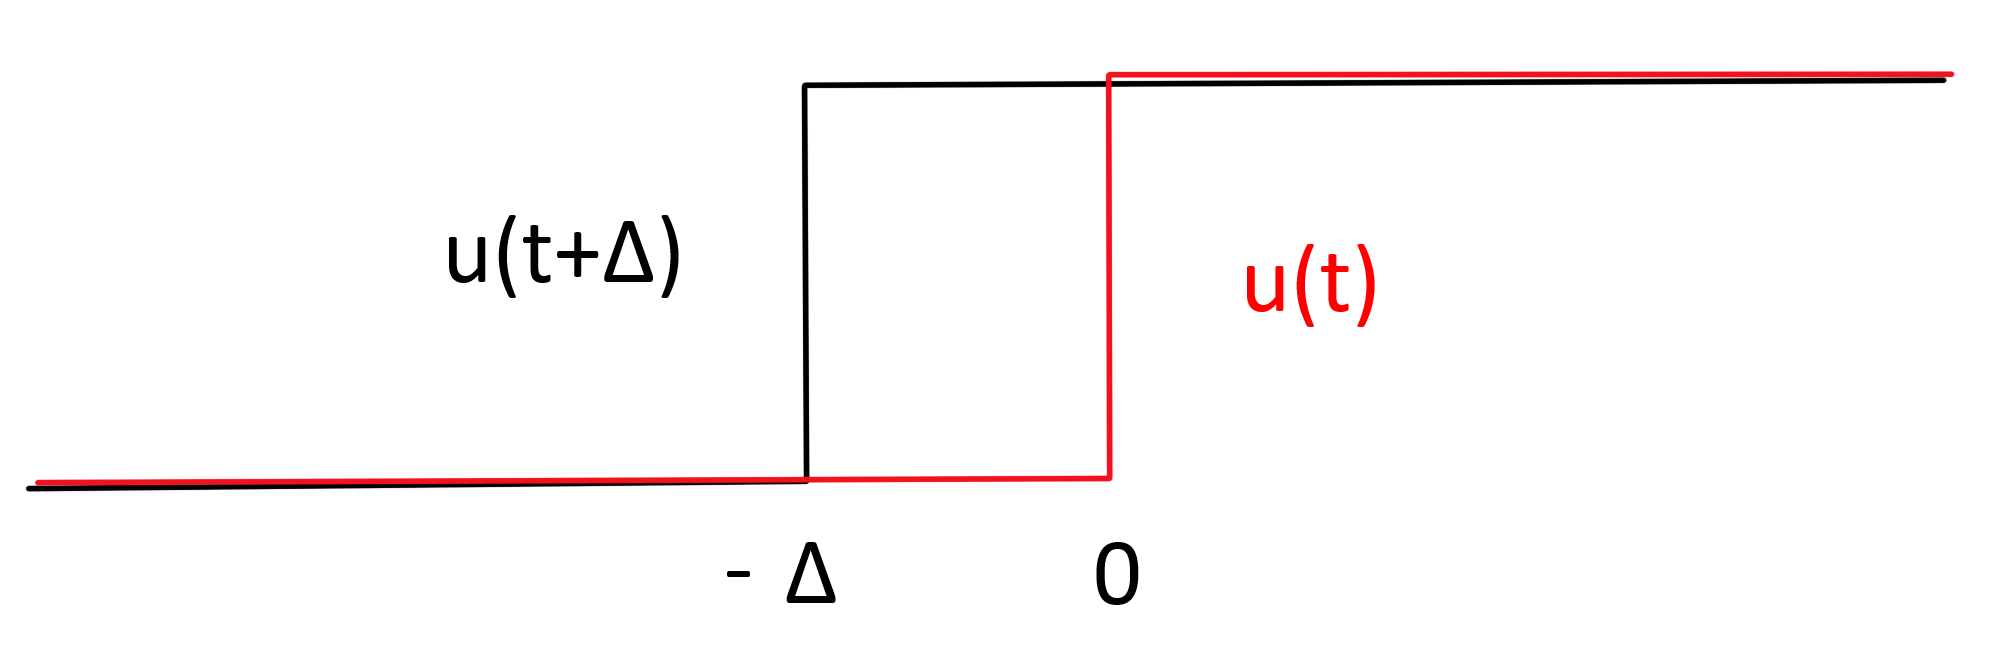
\includegraphics[width=0.6\textwidth]{./difference_deltas1.png}
	\caption{$u(t)$ and $u(t+\Delta)$}
\end{figure}
\indent	Now, talking their difference and dividing by $\Delta$ (fig. 3(b)), we get: 
\begin{figure}[H]
	\centering
	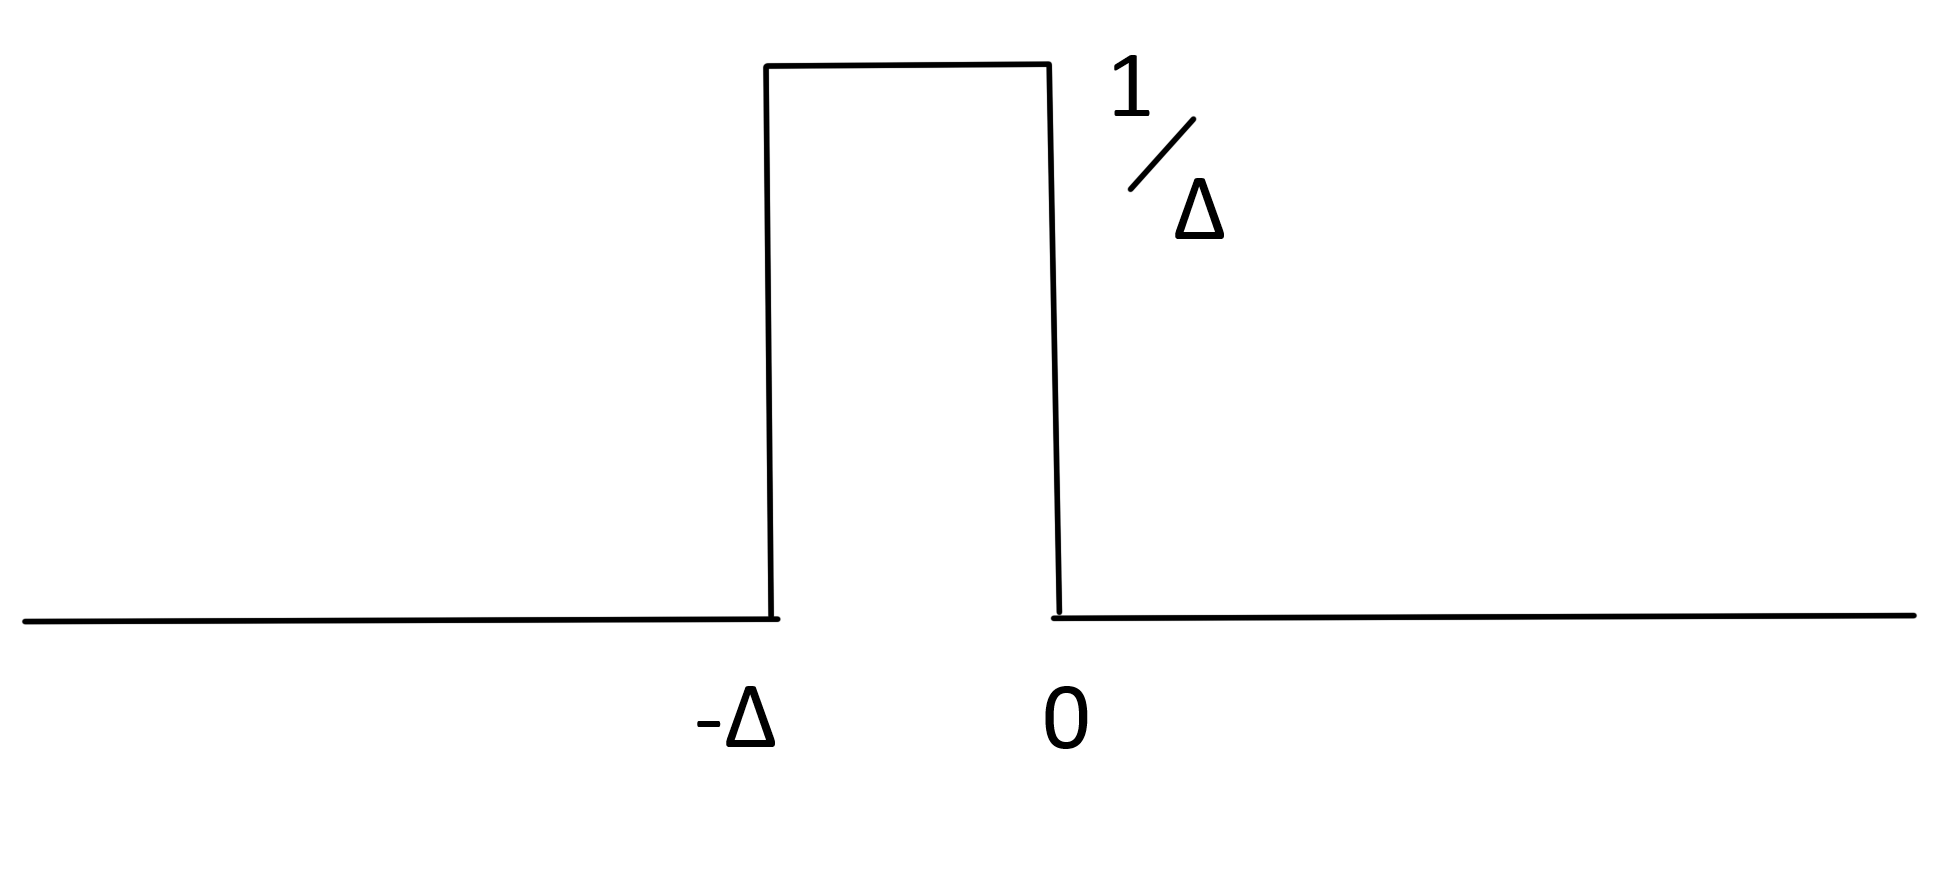
\includegraphics[width=0.6\textwidth]{./difference_deltas2.png}
	\caption{Difference of $u(t)$ and $u(t+\Delta)$, divided by $\Delta$}
\end{figure}
\indent which is nothing but the $\delta_\Delta$ function which we talked about. Taking the limit $\Delta\rightarrow0$, we get the derivative of $u(t)$ on one side, and the unit impulse $\delta(t)$ on the other.
Thus, there is a relationship of integration and differentiation between the unit step function and the unit impulse function. We have also found out the unit step response of the RC circuit. Since the derivative of the unit step function is the unit impulse function, is it true that the derivative of the unit step response for the RC circuit will give the unit impulse response?
More generally, if an input $x(t)$ produces an output $y(t)$ for an LSI system, does the derivative of $x(t)$ produce as the output, the derivative of $y(t)$?\\
\indent Intuitively, it seems to be correct, and taking the derivative of the unit step response for the RC circuit should give its unit impulse response. This question will be answered in the next lecture.

\section{Lecture 9: Unit Impulse Response of the RC circuit}


\subsection{Taking the derivative of the input signal for an LSI system}
Let \textbf{S} be a Linear Shift-Invariant system, and let $y(t)$ be the output corresponding to an input signal $x(t)$.\\
\indent Because of the Shift invariance of the \textbf{S}, $x(t+\Delta)$ will produce an output of $y(t+\Delta)$
\begin{figure}[H]
	\centering
	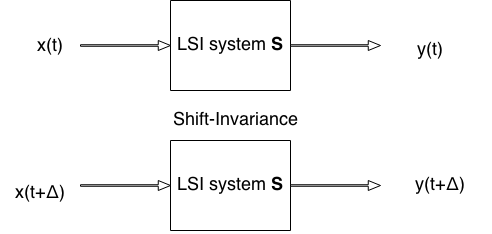
\includegraphics[width=0.6\textwidth]{shift_inv_1.png}
	\caption{Shift-invariance}
\end{figure}
\indent Homogeneity implies that $-x(t)$ will result in an output of $-y(t)$. And thus using additivity, an input of $x(t+\Delta)-x(t)$ will produce an output of $y(t+\Delta)-y(t)$.
\begin{figure}[H]
	\centering
	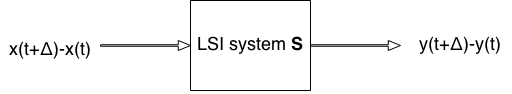
\includegraphics[width=0.6\textwidth]{ad_hom.png}
	\caption{Additivity and Homogeneity}
\end{figure}
\indent Invoking homogeneity with a scaling of $\frac{1}{\Delta}$, and taking the limit $\Delta\rightarrow0$, we obtain the result that the derivative of $x(t)$ produces the derivative of $y(t)$, as the output.
\begin{figure}[H]
	\centering
	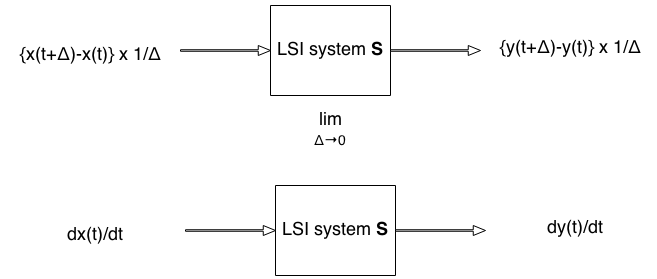
\includegraphics[width=0.8\textwidth]{derixt_deriyt.png}
	\caption{Scaling by $\Delta$ followed by taking the limit $\Delta\rightarrow 0$}
\end{figure}


\subsubsection{Impulse response of the RC circuit}
Now we can finally obtain the impulse response of the RC circuit. To do this, we need to apply the result of the previous section to the the unit step response of the RC circuit. As discussed previously, the unit step response of the RC circuit is the function $s(t)=(1-e^{-\frac{t}{\tau}})u(t)$.\\
\indent Now, since the RC circuit is an LSI system, the derivative of $u(t)$ should produce the derivative of $s(t)$! But we already know that the derivative of the unit step function is the unit impulse. Thus the unit impulse response is nothing but the derivative of the unit step response $s(t)$!\\
Using the product rule for differentiation, we get
\begin{eqnarray*}
\frac{ds(t)}{dt} &=& u(t)\Big\{\frac{d}{dt}(1-e^{-\frac{t}{\tau}})\Big\} + (1-e^{-\frac{t}{\tau}})\frac{du(t)}{dt}\\
&=& \frac{1}{\tau}e^{-\frac{t}{\tau}}u(t)+(1-e^{-\frac{t}{\tau}})\delta(t)
\end{eqnarray*}
\indent Now note that the second term in the expression is the delta function multiplied by another function. But $f(t)\delta(t)=f(0)\delta(t)$. The second term in the above equation vanishes, since f(0)=0 in this case. Thus we obtain,
$$\frac{ds(t)}{dt}=\frac{1}{\tau}e^{-\frac{t}{\tau}}u(t)$$
This is the formula for the Impulse Response of an RC circuit.
\subsubsection{Interpretation of the RC unit Impulse Response}
We can try to understand how this result makes sense physically.\\
\indent Applying a unit impulse voltage across the RC voltage is like suddenly pumping in an amount of charge into the circuit. Let us use the $\delta_\Delta$ function instead of the the unit impulse, since it is easier to interpret applying a finite voltage $\frac{1}{\Delta}$ over a finite time $\Delta$. Since the voltage across a capacitor does not behave in an `impulsive' manner, this sudden jump in the voltage at $t=0$ is sustained by the resistor R, setting up a current:
$$I=\frac{1}{\Delta}.\frac{1}{R}$$
Now, at the same time, the same current flows through the Capacitor, and integrating this current gives us the capacitor charge:
$$\textrm{Capacitor Charge}=\Delta .\frac{1}{\Delta} .\frac{1}{R}$$
Resulting in a voltage across the Capacitor (at time $t=0$ ):
\begin{eqnarray*}
\textrm{Capacitor Voltage at time t=0}&=&\Delta .\frac{1}{\Delta} .\frac{1}{R} .\frac{1}{C} \\
&=&\frac{1}{RC}\\
&=& \frac{1}{\tau}
\end{eqnarray*}
\indent Since there is no applied voltage across the circuit after $t=0$, the capacitor simply discharges exponentially, thus giving us :
\[
\textrm{Capacitor voltage, i.e. output voltage}=\frac{1}{\tau}e^{-\frac{t}{\tau}}u(t) 
\]
%\tag{3.1.1a,b}
	
\section{Lecture 10: Introduction to Discrete Systems}



\subsection{Introduction}

In the previous sessions, we have learnt about the continuous time systems. We also studied the different properties of these systems like additivity, homogeneity, shift invariance and so on.
We are no able to identify whether a given continuous time system is additive or shift invariant or homogenous or not. 
However, all these parameters were studied only with respect to a certain type of systems i.e, Continuous Time Systems. These are the systems where the independent variable is continuous and the signal is defined for a continuous range of values.
We will now look at a different type of systems i.e, the Discrete ‘Independent Variable’ Systems.
It should be noted that a very important class if discrete signal arises from the sampling of continuous time signal.


\subsection{Definition}
 Systems where in the independent variable assumes only discrete values are known as discrete ‘independent variable’ systems. 

\paragraph{Examples}

A very well known example of this kind of system is the Stock Market Index. 
Another example could be that of a graph showing the scoring and run rate of a batting team in a cricket match.
\subsection{Representation}


Consider a co-ordinate system of only one axis. Now the discrete time system independent variable will only assume discrete values. Thus, the axis will have the co-ordinates separated by nT, where n is an integer and $T$ is the 'sampling time period' and can be  one second, one day, one year and so on. 

Once we decide ‘$T$’, only it's value matters. 

We shall represent a Discrete System as: 
$$X[n] \rightarrow Y[n]$$

We shall use the square brackets [] to show discreetness of the system.


\begin{figure}[ht]
\centering
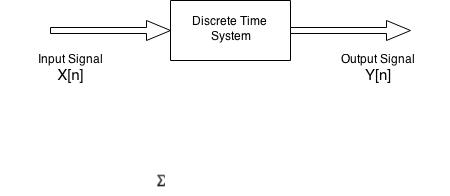
\includegraphics[width=0.7\textwidth]{Block_1.jpg}
\caption{\label{fig:Block_1}Discrete Independent Variable System Representation.}
\end{figure}


\subsection{Examples of a Discrete Time System}

\subsubsection{Example 1}
Consider a Bank Account. 

A certain amount $X[n]$ is deposited at a given time.


$T$ is the interval of interest calculation.


$Y[n]$ is the amount present at the $n$th instant.


The Bank gives an interest half yearly. Thus, a certain amount of interest is calculated after 6 months. The next amount is calculated over the next 6 months.

$\alpha$ is the rate of interest for the first 6 months while $\beta$ will be the rate of interest for the next 6 months. 

Thus if $\alpha$ and $\beta$ are the interest rates over two intervals of 6 months each.

The amount $Y[n]$ at the $n$th instant will be given as:

$$Y[n]=(\alpha.Y[n-1])+(\beta.Y[n-2])+X[n]$$

The amount $Y[n]$ will thus be the interest collected over the previous 2 intervals of 6 months each along with the current amount in the account $X[n]$.

This can be seen as an example of a Discrete System. 

Also, since the output is dependent on it's own past, it is a 'Recursive System'.


\subsubsection{Example 2}
Consider a Population in a region. 

We need to calculated the Tax Paid $Y[n]$ by this population. 

Population (Input) is given by $X[n]$.

The tax is paid over two intervals at the rates $\alpha$ and $\beta$.

The above system can be stated as:

$$Y[n]=(\alpha.X[n])+(\beta.X[n-1])$$

The above system out put or The Tax collected is Independent of it's previous state.

Hence above is a Non-Recursive System.



The Properties of Discrete Independent Variable systems will be studied in the following sessions.



\section{Lecture 11: Properties of Discrete Systems.}


\subsection{Additivity}

\subsubsection{Introduction}

Previously, we were introduced to a new form of systems that is, Discrete Independent Variable Systems. 
If we recall, we had established a fact that the properties of Discrete Systems are more or less similar to those of the Continuous Systems. In this session, we look at one of the properties of Discrete Systems i.e, Additivity. 



\subsubsection{Definition}
Additivity can be defined such that a system is said to be additive if the output corresponding to the sum of any two inputs is the sum of the two outputs.

Thus if we have two inputs to a given system X1[n] and X2[n], the output of the system will be Y[n]=Y1[n]+Y2[n]. This is very much like the continuous time system.

We must note that we are adding the entire signals and not just certain points of the signal. Thus, we are basically adding the entire sequence of signals. We refer to the signals as a sequence since in Discrete Systems, we can talk about a point before and a point after the given point.

\subsubsection{Proving Additivity}
Note that in order to prove that a given system is additive, we should prove that the system is additive for all the points in the sequence. 

Thus if we add the points X1[n]+X2[n] +…Xn[n] , in order to prove the given system is additive, the output has to be Y[n]=Y1[n]+Y2[n]+…..Yn[n].

$$\sum X[n]  \rightarrow \sum Y[n]$$

However, in order to prove that a given system is not additive, disproving the additivity at even two given points is enough.




\subsubsection{The Tax Example}
We could now look at the tax example which we had previously seen.

As we know, the tax collected is given by the equation :

$$Y[n] = { \alpha.X[n] +\beta. X[n-1] }$$
Here $\alpha$ and $\beta$ are the rates of taxation at the given instances.

In order to illustrate the additivity of this taxation system , let us consider two states S1 and S2 having the same tax rules. X1[n] and X2[n] are the populations of the two states in the nth interval respectively. 

Let S be the system that collects the tax. If we consider both the states together, we need to find the tax that is collected together.
\subsubsection{Proof}
$$X[n] = {X_1[n] + X_2[n] }$$
$$Y[n] = { \alpha.X[n] +\beta.X[n-1] }$$
$$Y[n] = { \alpha.X_1[n] +\alpha.X_2[n]+\beta. X_1[n-1]+\beta.X_2[n-1] }$$
$$Y[n] = { [{\alpha.X_1[n]+\beta. X_1[n-1]}] +[{\alpha.X_2[n]+\beta.X_2[n-1]}] }$$
$$Y[n] = {Y_1[n] + Y_2[n] }$$
The above will be true for any given X1[n] and X2[n].We thus conclude that the above system is additive.


\pagebreak

\subsection{Homogeneity and Shift Invariance.}

\subsubsection{Introduction}

We have looked at the Additive property of Discrete Systems previously. Continuing our discussion on properties, we now look at two new properties of Discrete Systems. Namely, Homogeneity and Shift Invariance. 


\subsection{Definition}
The properties of continuous as well as discrete systems seem to be more or less similar. However, there are minor differences in the way we define these properties.

\subsubsection{Homogeneity}
A Homogeneous system is defined as the one where if the input is scaled by a given constant, the output is also scaled by the same constant.


\subsubsection{Shift Invariance}
Shift Invariant system is defined as the one where if we shift the input by a given amount of time (or given number of samples in this case), the output will be shifted by the same amount of time (or number of samples). 

Note that in discrete systems, we can only shift the input by integral values unlike in continuous systems. 




\subsubsection{A Homogeneous System}

Consider a system with input X[n] , giving an output Y[n]. Now, we must note that in a discrete memory system, we map the whole input sequence on to the output sequence. It is not a point to point mapping which would make it memoryless. 

Thus, when we scale the given input signal by say a constant $\alpha$, for the system to be homogeneous the output will be scaled by the same constant $\alpha$. This is true for every possible input X[n] and every possible constant $\alpha$. 

$$X[n]\rightarrow Y[n]$$
$${\alpha.X[n]}\rightarrow {\alpha.Y[n]}$$

\subsubsection{Tax example with respect to a Homogeneous System}
We can now illustrate the tax system example taken a few sessions before. 

If we double the number of people in the state, the tax collected will also be doubled. 

Homogeneity insists that the output will be scaled by ‘the very same’ constant with which we scale the input. 


\begin{figure}
\centering

\end{figure}



\subsubsection{A Shift Invariant System}
Consider a discrete system, with an input $X[n]$, producing an output $Y[n]$. 

Now, if we shift the given input by an integer $D$, we have the input as $X[n-D]$. 

For the system to be shift invariant, it should produce an output which will be shifted by the same integer D.
$$X[n]\rightarrow Y[n]$$
$$X[n-D]\rightarrow Y[n-D]$$
Where D $\in$ Integer and the above holds true for every D and every X[n].

\subsubsection{Tax example with respect to a Shift Invariant System}
Going back to the taxation example, what Shift invariance implies is that the rate of the tax remains the same over several years.

So as we jump by a certain amount of time, the tax or the output Y[n] should continue to remain the same.


\todo[inline, color=white]{Note that Shift Invariance demands a lot from the system. Shift Invariant Systems are very rare in real life or are probably non-existent. A system could however be Shift Invariant over a long range of period. }

\pagebreak

\subsection{Causality}

\subsubsection{Introduction}

In our discussion on the Discrete Independent Variable systems, we have so far seen 3 properties. Namely Additivity, Homogeneity and Shift Invariance. We now look at another two properties, Causality and Stability. These discussion on the properties of Discrete Systems help us to understand how they are very much similar to the properties of Continuous Systems in nature. 

\subsubsection{Definition}
A system is Causal if the output at anytime depends only on the values of the input at the present time and in the past. 

Thus, if two inputs to a Causal System are identical up to some sample n0, the corresponding outputs must also be equal up to this point.

\subsubsection{A Causal System}
A causal System is also referred to as a non-anticipative system since the system output does not anticipate future values of the input. 

A real life example of a Causal system could be an RC circuit since a capacitor voltage depends only on the present and past values of the source voltage.

Looking at the definiton of a Causal System, we can represent it as follows:

If $$ X_1[n]=X_2[n]$$
upto $$n \leq n0$$,
A system is said to be causal if for all $X_1[n]$,$X_2[n]$,$n \leq n0$

$$ Y_1[n]=Y_2[n]$$



\subsection{Stability}

\subsubsection{Boundedness}
A bounded input can be defined as an input having a bounded maximum magnitude. If we have an input X[n], magnitude of the input will have a maximum value $Mx$ which will always be (strictly) less than $\infty$. 

The above can be represented as follows:
$$ X[n] \leq Mx < \infty$$


\subsubsection{Definition}
A system is defined to be Stable if every bounded input to the system results in a bounded output over the interval [$ n_0,\infty $] . 

This must hold for all initial samples. So, as long as we don't input $\infty$ to our system, we won't get $\infty$ output.


\subsubsection{A Stable System}

A Stable System is the one for which small inputs lead to responses that do not diverge. 
The input of a stable system is always bounded.
An example of a Stable System could be as follows:

$$Y[n]=(\frac{1}{2T+1})\sum_{k=-T}^{T} X[n-k]$$

We can see that as X[n] is a bounded value for all values of n by certain number $\beta$, then the largest possible magnitude of Y[n] will also be $\beta$.

This is because Y[n] is the average of a finite set of values of input. 

We looked at a few important properties of Discrete Independent Variable Systems in this Lecture. 
\section{Lecture 12: Impulse Response and Convolution}



\subsection{Introduction}

In the previous sessions, we have studied various properties of Discrete Systems. Two of these properties when combined are of great analytical importance and hence of great help. These are, Linearity and Shift Invariance.

In this session, we look at the combination of the above two systems, names as Linear Shift Invariant systems. 

\subsection{A Linear Shift Invariant System}
Consider a system "S" which is Linear Shift Invariant. We have already studied that $$ Linearity = Additivity + Homogeneity$$
Thus, a Linear Shift Invariant System will have the properties of:
\begin{enumerate}
\item Additivity
\item Homogeneity
\item Shift Invariance
\end{enumerate}

In order to study the various input-output characteristics of a Linear Shift Invariant System, we could apply a certain known input function namely a 'Unit Impulse Response' Sequence. 


\subsubsection{Unit Impulse Response}
An impulse is a sudden, shortlived phenomenon.

A Unit Impulse Response sequence can be defined as the sequence which has just one finite value '1' at the origin and 'zero' else where.

Mathematically it can be written as:
$$ \delta[n] = 1, n=0$$
$$ \delta[n] = 0, n \neq 0 $$

\subsubsection{Taxation system as a Linear Shift Invariant System}
we had earlier seen the taxation system. We had the tax collected as Y[n] given by
$$Y[n] = { \alpha.X[n] +\beta. X[n-1] }$$
\subsubsection{Additivity}
We have already proven that the given system is Additive in the previous session. 

Now, in order to find out if the given system is Linear Shift Invariant, we need to check for Homogeneity as well as Shift Invariance.

\subsubsection{Homogeneity}
In order to prove that the system is Homogenous, we can scale the input $X[n]$ by a constant $\gamma$

$$X[n] = \gamma.X[n]$$
Therefore, $$Y[n] = { \alpha.X[n] +\beta. X[n-1] }$$
$$Y[n] = { \alpha.\gamma.X[n] +\beta.\gamma. X[n-1] }$$
$$Y[n] = \gamma .({ \alpha.X[n] +\beta. X[n-1] })$$
$$Y[n] = \gamma.Y[n]$$

Hence we prove that the Tax system is Homogenous.

\subsubsection{Shift Invariance}
To prove that the system is Shift Invariant, we Shift the input by an integer'D'.

$$X[n] = X[n-D]$$
Therefore, $$Y[n] = { \alpha.X[n] +\beta. X[n-1] }$$
$$Y[n] = { \alpha.X[n-D] +\beta. X[n-1-D] }$$
$$Y[n] = Y[n-D]$$

Thus we can see that the Taxation System is
\begin{itemize}
\item Additive
\item Homogenous
\item Shift Invariant
\end{itemize}

The Taxation System is thus found out to be an example of a 'Linear Shift Invariant' System.

\begin{figure}
\centering
\end{figure}





\subsubsection{Unit Impulse Response of a Linear Shift Invariant System}
Consider a Unit Impulse Sequence given as an input to a Linear Shift Invariant System. 
Input is given as $\delta[n]$
Therefore, $$Y[n] = { \alpha\delta[n] +\beta \delta[n-1] }$$
Now, we know that $\delta[n]=1 at n=0$
Hence we find that
$$Y[n]=\alpha $$ n=0
$$Y[n]=\beta $$ n-1=0 or n=1
$$Y[n]=0 $$ $n \neq 0$

Thus the tax collected or the output Y[n] will have only two discrete values. 

We thus analyze the unit impulse response of a Linear Shift Invariant System. 



\subsection{Theorem}
The theorem for Discrete Linear Time Invariant System states that 'the unit impulse response characterizes the system completely.

The above theorem states that given the unit impulse response of a system, it is possible to determine the output Y[n] for an input X[n].
 

\pagebreak

\chapter{The Impulse Response for Discrete LSI Systems}

\setcounter{section}{0}

\subsection{Introduction}
The input output relation of a Linear Time Invariant system can be found out if we know it's unit impulse response. 

We have formally stated this in a theorem that 'the unit impulse response characterizes the system completely.' 

We will look at the proof of the above theorem in this session.

\subsection{Proof of the Theorem}
Considering the theorem, we can say that we know that for a given LSI System for a given input $ X[n]=\delta[n]$ the output will be $Y[n]=h[n]$.

We shall now look at the proof step by step:


\subsubsection{Linear Combination of a Sequence}
Consider an input sequence

$$X[n]= [3, 2, -4, 7]$$
Consider 2 as the sample at the origin.


Thus, $X[-1]=3, X[0]=2, X[1]=-4, X[2]=7$.

The above sequence can be written as a combination of unit impulses of different magnitudes.

$$ X[n]= 3\delta[n+1] + 2\delta[n] - 4\delta[n-1] + 7\delta[n-2]$$
Therefore, 
$$ X[n]= X[n+1]\delta[n+1] + X[n]\delta[n] - X[n-1]\delta[n-1] + X[n-2]\delta[n-2]$$
$$X[n]=\sum_{k=-\infty}^{\infty} x[k]\delta[n-k]$$

\subsubsection{Shift Invariance}
We will now recall the properties of a LSI System. 
$X[n]=\delta[n]$
Since given system is Shift Invariant,
$\delta[n-D]\rightarrow h[n-D]$

\subsubsection{Homogeneity}
A LSI System is Homogeneous.
For a given value of $k$, the value of $X[k]$ will be constant.
scaling the impulse, shifted input by $X[k]$
Thus, $$X[k]\delta[n-k]\rightarrow X[k]h[n-k]$$

\subsubsection{Additivity}
LSI System shows the property of Additivity. 
$$\sum_{k=-\infty}^{\infty} X[k]\delta[n-k]\rightarrow \sum_{k=-\infty}^{\infty} X[k]h[n-k]$$


The term $'\sum_{k=-\infty}^{\infty} x[k]*\delta[n-k]'$ is nothing but $X[n]$ as seen above.

We can now conclude that the output of the system will be definitely known because of the earlier 3 properties discussed.

Therefore,$$Y[n]=\sum_{k=-\infty}^{\infty} X[k].h[n-k]$$

Hence we prove the theorem "constructively". That is, we now constructively and definitively know the input-output relation once we know the impulse response of the given LSI system.

\subsection{Introduction to Convolution}
The previously obtained output $Y[n]$ is obtained by 'convoluting' $X[n]$ and $h[n-k]$. 

This operation that is carried out between the two sequences is known as convolution. 

\pagebreak
\chapter{Discrete Convolution}

\setcounter{section}{0}

\subsection{Introduction}

Earlier we saw the concept of Convolution of two Sequences of Signals. 

Convolution is basically an operation between the two sequences which enables us to find out the output sequence. 

\subsection{Definition}
Convolution can be strictly defined as the operation between the input signal $X[n]$ and the impulse response $h[n]$ that results in the output $Y[n]$

$$Y[n]=X[n]*h[n]$$
In the above form, the $'*'$ term denotes Convolution. 
Therefore, $$Y[n]=\sum_{k=-\infty}^{\infty} X[k].h[n-k]$$


Note: The symbol $*$ will henceforth always refer to Convolution of two signals and NOT just simple multiplication.

\subsection{Procedure for Convolution}
\subsubsection{Applying the Input Signal}

\begin{figure}[ht]
\centering
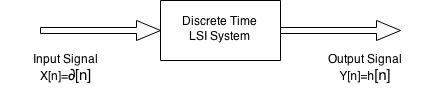
\includegraphics[width=0.5\textwidth]{Block.jpg}
\caption{\label{Step 1:} Applied input $X[n]=\delta[n]$}
\end{figure}


\subsubsection{Delaying the Input Signal}

\begin{figure}[ht]
\centering
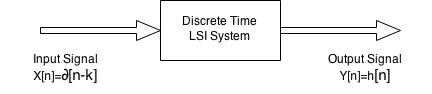
\includegraphics[width=0.5\textwidth]{Block_delay.jpg}
\caption{\label{Step 2:} Applied delay to the signal}
\end{figure}
\pagebreak



\subsubsection{Scaling the delayed Input Signal}

\begin{figure}[ht]
\centering
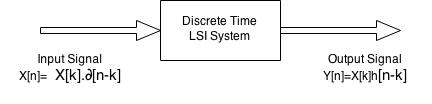
\includegraphics[width=0.5\textwidth]{Block_scale.jpg}
\caption{\label{Step 3:} Scaling the input by X[k]}
\end{figure}

\subsubsection{Adding the Scaled Impulses over the entire Range}

\begin{figure}[ht]
\centering
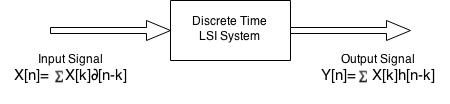
\includegraphics[width=0.5\textwidth]{Block_sum.jpg}
\caption{\label{Step 4:} Summing the input over the entire region}
\end{figure}


\subsection{Applications}
A few Applications of Convolution are listed below:
\begin{itemize}
\item To obtain the response (or output) signal of the discrete time signal input applied.
\item To obtain overall impulse response signal $h[n]$ for interconnected systems.
\item To determine similarity (co-relation) between the transmitted and reflected (or received) signal.This is also called as Auto-Corelation.
\item To obtain similarity between 2 different signals. Also called Cross-Corelation. 
\end{itemize}


\subsection{Examples on Convolution}
\subsubsection{Example 1:}

Calculate the output Y[1] for 
$$X[n]=[3,1,2]\hspace{10mm}X[0]=3$$
$$h[n]=[3,0,2]\hspace{10mm}X[0]=3$$

To find out $Y[1]$, replace $n$ by 1 in the Convolution formula.

$$Y[1]=\sum_{k=-\infty}^{\infty} X[k].h[1-k]$$

The signal sequence $h[1-k]$ will be represented as:
$$h[1-k]=[2,0,3]\hspace{10mm}h[0]=0$$

While Convoluting 2 sequences, as we have seen in Continuous Time domain, we need to find the part of the signal sequences that overlap. 

Therefore,
$$Y[1]=(X[0].h[o])+(X[1].h[1])$$
$$Y[1]=(3.0)+(1.3)$$
$$Y[1]=3$$

Thus we Convolve the signal sequences $X[n]$ and $h[n]$ in order to find the output $Y[n]$ at the point $n=1$.

\subsection{Properties of Convolution}
\subsubsection{Commutativity}
If, $$Y[n]=X[n]*h[n]$$

Then, by the Commutative Property of Convolution, 
$$Y[n]=h[n]*X[n]$$

\subsubsection{Distributivity}

If, $$Y[n]=X[n]*(h_1[n]+h_2[n])$$

Then, by the Distributive Property of Convolution, 
$$Y[n]=X[n]*h_1[n]+X[n]*h_2[n]$$

\subsubsection{Associativity}

If, $$Y[n]=X[n]*(h_1[n]*h_2[n])$$

Then, by the Associative Property of Convolution, 
$$Y[n]=(X[n]*h_1[n])*h_2[n]$$






\section{Lecture 13: Causality of LSI systems}




\subsection{Associativity and Commutativity of LSI Systems}
Two more properties of system, namely associativity and commutativity are explored here. These properties are not "new" in the sense that some basic operations like addition and multiplication follow these properties.
Note: Both discrete and continuous systems are considered together in the following discussion.

\subsubsection{Associativity}
\begin{figure}[ht]
\centering
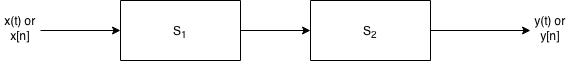
\includegraphics[width=0.8\textwidth]{cascade1.jpg}
\end{figure}

In the above image, we input signal $x$, either $x(t)$ for continuous system or $x[n]$ for discrete one, to LSI system $S_{1}$( having its impulse response $h_{1}(t)$ or $h_{1}[n]$), which can be considered continuous or discrete, depending on the case. The output of system $S_{1}$ is fed to LSI system $S_{2}$( having its impulse response $h_{2}(t)$ or $h_{2}[n]$), which also can be continuous or discrete. The output of $S_{2}$ is $y$, either $y(t)$ or $y[n]$ in continuous and discrete case respectively. That is, the whole setup can be considered either of the continuous or the discrete case. In the continuous case, both the systems as well as the relevant signals are continuous, whereas in discrete case they all operate on a discrete independent variable.\\
Note here, that the output obtained from the first system is $(x*h_{1})$, continuous or discrete. As this signal is fed to the $S_{2}$, we get output as 
\begin{equation}
y=(x*h_{1})*h_{2} \nonumber
\end{equation}

Now Associativity talks about the equivalence of systems put in series or cascade. Mathematically,
\begin{equation}
(x*h_{1})*h_{2}=x*(h_{1}*h_{2}) \nonumber
\end{equation}

Now if we have a LSI system $S_{3}$, whose impulse response is $h_{1}*h_{2}$, then from above equation it is clear that it will act exactly like these two systems $S_{1}$ and $S_{2}$ would have acted when applied in series. This is the physical significance of the associativity.\\

\begin{figure}[ht]
\centering
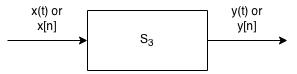
\includegraphics[width=0.5\textwidth]{eqv.jpg}
\end{figure}

So  in short, if we put two systems in a cascade, we can replace them with one single system whose impulse response is equal to the convolution of the impulse responses of these two systems.

\subsubsection{Commutativity}

Let us apply signal $x$ to system $S_{1}$ and then its output to system $S_{2}$, both LSI, to get output as $y$. Commutativity states that the order in which these systems come is irrelevant to the result i.e. we will get the same output in both the cases.  It states that regardless of which of the two systems comes first, the output $y$ is going to be the same.\\

\begin{figure}[ht]
\centering
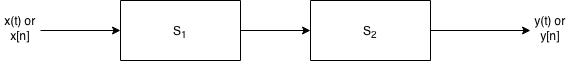
\includegraphics[width=0.8\textwidth]{cascade1.jpg}
\end{figure}
\begin{figure}[ht]
\centering
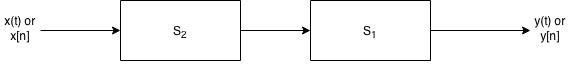
\includegraphics[width=0.8\textwidth]{cascade2.jpg}
\end{figure}

So the equivalent system which we talked about in the Associativity, is unaffected if the order of these two systems is reversed.\\\\

We can also generalize this to n cascaded LSI systems and say that for any permutation of the given n systems, the output is going to be the same. The proof of this is a bit more intricate and is left an as exercise to the student. The proof can be done by using the method of mathematical induction.

\subsubsection{What if my systems are not LSI?}

All of the above discussion is based on the assumption that all the systems we are considering are LSI in nature. While it may be tempting to generalize these seemingly simple results to all systems, and many times we tend to forget to confirm that the system in question is LSI or not before applying such properties, we must be careful. \\
It turns out that the commutativity and associativity may not hold if the systems $S_{1}$ and $S_{2}$ are not both LSI. For example,\
Let's say system $S_{1}$ is given by the equation $y(t)=(x(t))^2$ and $S_{2}$ by $y(t)=x(t)+1$. We have taken here continuous variable signals and systems, but the same discussion is valid for the discrete case as well. So if we apply first $S_{1}$ and then $S_{2}$, we will get $y(t)=(x(t))^2 +1$ as the output, while reversing the order, i.e. first applying $S_{2}$ and then $S_{1}$ would yield $y(t)=(x(t)+1)^2$. So the both outputs are clearly different.\\
But this does not mean that we can hurry and conclude that the resultant systems will {\it never} be the same. Consider, say, $S_{1}$ as $y(t)=x(t)+4$ and $S_{2}$ as $y(t)=x(t)-4$. Now in this case, regardless of which system comes first, we get output $y(t)=x(t)$.\\
Basically, if even one of the systems is not LSI, we cannot say anything about whether those systems follow associativity or commutativity beforehand: we must examine those systems carefully and determine the answer for the individual case.


\subsection{Causality of a Linear Shift Invariant System from its Impulse Response}

We have noted before that a LSI system can be represented by its impulse response, i.e. we know everything about a system once we know its impulse response. We have seen system properties like causality and stability: according to the previous statement, we should be able to know whether a system is stable and/or causal just by looking at and examining its impulse response. The conditions turn out to be very similar for continuous and discrete variable systems and their respective impulse responses.

\subsubsection{Causality of continuous variable LSI systems}

We say that a system is causal when its output depends only on the past and the current inputs, and {\it not} on the future inputs. We know that, for a continuous independent variable system $S$` having impulse response $h$t, we can relate its input and output by the equation
\begin{equation}
y(t)=\int_{-\infty}^{+\infty} h(\tau)x(t-\tau)\,d\tau \nonumber
\end{equation}

Note that as $\tau$ goes from ${-\infty}$ to ${+\infty}$, $t-\tau$ also goes from ${-\infty}$ to ${+\infty}$. Note that $\tau$ being positive corresponds to the past ( as $t-\tau < t$ when $\tau$ is positive and '$t$' is the current timeframe) while $\tau$ negative to the future and 0 to the current time. Now for the system being causal, we want to eliminate the future inputs, so we must have $h(\tau)$ 0 when $\tau$ is negative, so that there's no contribution of the future terms to the $y(t)$, the output. Note that $h(\tau)=0$ when $\tau<0$ is sufficient condition for causality of the system. It is easy to prove that this condition is also necessary for the system to be causal i.e. there can be no system which is causal that violates this condition. The proof can be done by using the method of proof by contradiction.

\subsubsection{Causality of discrete variable LSI systems}

For discrete systems, we have the following equation relating output to the input(s):
\begin{equation}
y[n]=\sum_{\kappa=-\infty}^{+\infty} h[\kappa]x[n-\kappa] \nonumber
\end{equation}
Similar to the argument for the continuous case, $\kappa<0$ corresponds to the future, $\kappa>0$ to the past and $\kappa=0$ to the present/current input. So causality will be ensured if all the future inputs are cut off, i.e. $h[\kappa]=0,\, \forall \kappa<0$. This is the sufficient condition for  system to be causal. We can also prove the sufficiency by one more way:\\
Consider signals $x_{1}[n]$ and $x_{2}[n]$ such that $x_{1}[n]=x_{2}[n]\, \forall n \le n_{0}$.\\ Note that $x_{1}[n]$ may not be the same as $x_{2}[n]$ for any $n \geq n_{0}.$ Also, from given condition( we are assuming the condition we arrived at to reach at the conclusion that the system is causal)  $h[\kappa]=0 \forall \kappa<0$\\
Now if the system is causal, we must be able to reach  $y_{1}[n]=y_{2}[n]\, \forall n \le n_{0}$.\\
Consider
\begin{equation}
y_{1}[n]=\sum_{\kappa=0}^{+\infty} h[\kappa]x_{1}[n-\kappa],  n \le n_{0} \nonumber
\end{equation}
Note that we started the sum from 0 as before zero, in$-\infty$ to 0 region, we already know that  $h[\kappa]=0$.
Now observe the summation. it contains $x_{1}[n-\kappa]$. But as $\kappa$ is less than 0, we have $n-\kappa>n$, or  $x_{1}[n-\kappa]= x_{2}[n-\kappa]$.\\
So the sum can be converted to 
\begin{equation}
y_{1}[n]=\sum_{\kappa=0}^{+\infty} h[\kappa]x_{2}[n-\kappa] \nonumber
\end{equation}
And the right hand side of the equation is essentially $y_{2}[n]$.\\
Hence  $y_{1}[n]=y_{2}[n] \forall n \le n_{0}$. Hence the sufficiency of the condition is proved. The necessity can also be proved, by using proof by contradiction.

\section{Lecture 14: Conditions for Stability}



Let us try to see whether system is stable or not, from its impulse response. First we will discuss about the discrete case, and then move on to continuous variable case. In both cases, that a system is stable means it gives a bounded output for every bounded input, or a bounded input signal always yields a bounded signal as an output.
\subsection{Stability of LSI system from it's impulse response: Discrete variable.}
 For discrete variable systems, output is related to the input by the following equation:
\begin{equation}
y[n]=\sum_{\kappa=-\infty}^{+\infty} h[\kappa]x[n-\kappa] \nonumber
\end{equation}
As we are concerned whether output is bounded or not, we need to look at the modulus of the output, i.e.
\begin{equation}
|y[n]|=|\sum_{\kappa=-\infty}^{+\infty} h[\kappa]x[n-\kappa]| \nonumber
\end{equation}
But we know that, in general,
\begin{equation}
|\sum a_{i}| \le \sum|a_{i}| \nonumber
\end{equation}
So 
\begin{equation}
|y[n]|\le\sum_{\kappa=-\infty}^{+\infty} |h[\kappa]x[n-\kappa]| \nonumber
\end{equation}
Or,
\begin{equation}
|y[n]|\le\sum_{\kappa=-\infty}^{+\infty} |h[\kappa]||x[n-\kappa]| \nonumber
\end{equation}
BUt we know that the input signal is bound, say $x[n] \le M_{x}, \forall n$. So
\begin{equation}
|y[n]|\le M_{x}\sum_{\kappa=-\infty}^{+\infty} |h[\kappa]| \nonumber
\end{equation}
Clearly, if $\sum_{\kappa=-\infty}^{+\infty} |h[\kappa]|$ is finite, then $|y[n]|$ is finite. This is the sufficient condition for a system to be stable. The quantity $\sum_{\kappa=-\infty}^{+\infty} |h[\kappa]|$ is called as the 'absolute sum' of $h$.\\
In general, if we have a sequence $\{ a_{n}\}$ then the quantity  $\sum_{\kappa=-\infty}^{+\infty} |\{ a_{n}\}|$ is called as the absolute sum of sequence $\{ a_{n}\}$. In short, we take the absolute value of the each term of the sequence, and add those to get the absolute sum of a sequence.\\
If indeed $h[n]$ is absolutely summable, i.e. its absolute sum is a finite number/absolute sum is convergent, then we can say for some $ M_{h}$ lying between $0$ and $\infty$,
\begin{equation}
 \sum_{\kappa=-\infty}^{+\infty} |h[\kappa]|\le M_{h} \nonumber
\end{equation}
So our output in that case becomes
\begin{equation}
|y[n]| \le M_{x}M_{h} \nonumber
\end{equation}
This is very important. It means that the sufficiency condition which we have is a constructive condition. It not only tells that the output is bounded, but also talks about its bound.




\subsection{Stability of LSI system from it's impulse response: Continuous variable.}
 For continuous variable systems, output is related to the input by the following equation:
\begin{equation}
y(t)=\int_{-\infty}^{+\infty} h(\tau)x(t-\tau)\,d\tau \nonumber
\end{equation}
As we want to discuss about the boundedness of $y(t)$, we will take modulus on both sides:
\begin{equation}
|y(t)|=|\int_{-\infty}^{+\infty} h(\tau)x(t-\tau)\,d\tau| \nonumber
\end{equation}
Using the identity
\begin{equation}
|\int f(x) dx| \le \int|f(x)| dx \nonumber
\end{equation}
We get
\begin{equation}
|y(t)|\le\int_{-\infty}^{+\infty}| h(\tau)x(t-\tau)\,|d\tau \nonumber
\end{equation}
So
\begin{equation}
|y(t)|\le\int_{-\infty}^{+\infty}| h(\tau)||x(t-\tau)\,|d\tau \nonumber
\end{equation}
But we know that, as input $x(t)$ is bounded,
\begin{equation}
|x(t)| \le M_{x} \quad \forall t, 0 \le M_{x}< \infty \nonumber
\end{equation}
So 
\begin{equation}
|y(t)|\le\int_{-\infty}^{+\infty}| h(\tau)|M_{x}\,d\tau \nonumber
\end{equation}
We observe that, $y(t)$ will be bounded if $\int_{-\infty}^{+\infty}| h(\tau)|\,d\tau$ is bounded. And that is the sufficient condition for a continuous variable system to be stable. Now this integral $\int_{-\infty}^{+\infty}| h(\tau)|\,d\tau$ is called the 'absolute integral' of $h(\tau)$, similar to the absolute sum.\\
In this case also, we can estimate the bound on the output as follows:\\
Let
\begin{equation}
\int_{-\infty}^{+\infty}| h(\tau)|\,d\tau \le M_{h}. \nonumber
\end{equation}
Substituting this in the equation we got for the output,
\begin{equation}
|y(t)|\le M_{x}M_{h} \nonumber
\end{equation}\\\\
Note that, we have discussed here only the sufficiency of the conditions for the stability of systems, both discrete and continuous. We still need to ponder upon whether these conditions are necessary for a system to be stable.


\subsection{Necessity of the condition for stability}
We will now discuss about the necessity of the condition for the stability for discrete variable systems. The proof for continuous variable systems is very similar. We will assume that the output obtained from a system, $y[n]$, when it receives a bounded input is also bounded, i.e.
\begin{equation}
|y[n]| \le M_{y} \quad \forall n, 0 \le M_{y}< \infty \nonumber
\end{equation}
And try to reach at the necessary condition we had earlier got, i.e. try to prove that the absolute sum of $h[n]$ is finite. For that, we will give a specific bounded input to the system, and observe output at a specific point, which should also be bounded if we indeed have a stable system( from our assumption). We know that the input and output for a discrete variable system are related through the following equation:
\begin{equation}
y[n]=\sum_{\kappa=-\infty}^{+\infty} h[\kappa]x[n-\kappa] \nonumber
\end{equation}
Now consider that we are looking at the output when $n$ is equal to zero. So the equation now becomes
\begin{equation}
y[0]=\sum_{\kappa=-\infty}^{+\infty} h[\kappa]x[-\kappa] \nonumber
\end{equation}
Basically we are trying to bring the absolute sum as an output for some suitable input, which is bounded, and once it is done, we will have proven the necessity of the condition for stability. And the input we choose to give to the system is the following:
\begin{eqnarray*}
x[n]&=&\frac{\overline{h[-n]}}{|h[-n]|}\quad , if h[-n]\neq 0 \\
       &=&0                         \quad   \quad \quad, if h[-n]=0
\end{eqnarray*}
Where $\overline{h[-n]}$ is the complex conjugate of $h[-n]$. So when we apply it in the equation, it becomes
\begin{eqnarray*}
n=-\kappa\quad So\\
x[-\kappa]&=&\frac{\overline{h[\kappa]}}{|h[\kappa]|}\quad , if h[\kappa]\neq 0 \\
       &=&0                         \quad   \quad \quad, if h[\kappa]=0
\end{eqnarray*}
So we have the equation
\begin{equation}
y[0]=\sum_{\kappa=-\infty}^{+\infty} h[\kappa]x[-\kappa] \nonumber
\end{equation}
After substituting $x[-\kappa]$, it becomes
\begin{eqnarray*}
y[n]&=&\sum_{\kappa=-\infty}^{+\infty}\frac{h[\kappa]\overline{h[\kappa]}}{|h[\kappa]|}\quad , if h[\kappa]\neq 0 \\
       &=&\quad\quad\quad0                         \quad \quad  \quad \quad, if h[\kappa]=0\\
       &=&\sum_{\kappa=-\infty}^{+\infty}|h[\kappa]|
\end{eqnarray*}
Which is the absolute sum of the impulse response. Now as $y[n]$ is bounded, $y[0]$ must be finite and so must be the absolute  sum. Hence we have proved the necessity of the absolute sum of the impulse response being finite for the system being stable. The proof for the continuous variable systems is very similar. It is left to you as an exercise.

\section{Lecture 15: Introduction to Convolution}



\subsection{Input Output Relationship in LSI Systems: the Impulse Response}
We have studied several properties of the systems, both continuous and discrete. One very important concept amongst them is the impulse response for the LSI systems which not only showed us how we can obtain the output from the input for the system, but also the properties of that system. It's a very peculiar relation, which relates the input to the output though. So let us try to study it further: and see how we go about doing that somewhat-complicated looking summation or integral. Here are the expressions, both of summation for the discrete systems and integral for continuous ones, for our reference:\\
For discrete systems, we'd write:
\begin{equation}
y[n]=\sum_{\kappa=-\infty}^{+\infty} x[\kappa]h[n-\kappa] \nonumber
\end{equation}
And for continuous systems,
\begin{equation}
y(t)=\int_{-\infty}^{+\infty} x(\tau)h(t-\tau)\,d\tau \nonumber
\end{equation}
Doesn't it look very similar? The operation we are performing on the input signal $x$ is essentially the same, the only difference is the difference between an integral and a summation, which comes from the nature of the independent variable: whether that variable is discrete or continuous. So lets examine this operation carefully. How do we actually perform it? Let's take the simpler version of the summation first:\\ 
Consider following $x[n]$:
\begin{eqnarray*}
x[n] &=& -1, \quad\, n=-1 \\ 
&=& 9, \quad\quad n=0\\
&=& 5, \quad\quad n=1\\
&=& 3, \quad\quad n=2\\
&=& 0, \quad\quad otherwise
\end{eqnarray*}
and $x[n]$ is zero elsewhere.
\subsubsection{Arrow Notation for writing $x[n]$ Conveniently}
We have represented x[n] above, but this way seems a little bit tedious. So we introduce a new neat notation to write finite-length discrete signals, called the arrow notation. We basically write the out all of the values $x[n]$ takes, as $n$ changes, and indicate $n$ corresponding to any one of the values. So we'd write the same signal in arrow notation as:\\
%\begin{table}[h]
%\centering
\begin{tabular}{ l  c r r r }
  $x[n] =$ & -1 & 9 & 5 & 3 \\
   &  & $\uparrow$ &  & \\
   &  & 0 &  & \\
\end{tabular}\\
%\end{table}
Now instead of zero, it may as well have been any other number. For example,\\
%\begin{table}[h]
%\centering
\begin{tabular}{ l  c r r r }
  $x[n] =$ & -1 & 9 & 5 & 3 \\
   &   $\uparrow$& &  & \\
   &   -1& &  & \\
\end{tabular}\\
%\end{table}
is an equally valid expression. The output is assumed to be zero everywhere else, at the points which are not shown.

\subsection{Getting the output for a discrete system}
So, back to our finding the output: we have the $x[n]$:\\
%\begin{table}[h]
%\centering
\begin{tabular}{ l  c r r r }
  $x[n] =$ & -1 & 9 & 5 & 3 \\
   &  & $\uparrow$ &  & \\
   &  & 0 &  & \\
\end{tabular}\\
%\end{table}
And $h[n]$:\\
%\begin{table}[h]
%\centering
\begin{tabular}{ l  c r r  }
  $h[n] =$ & 1 & -1 & 2\\
     & $\uparrow$ &  & \\
     & 0 &  & \\
\end{tabular}\\
%\end{table}
We want to find $y[n]$, where
\begin{equation}
y[n]=\sum_{\kappa=-\infty}^{+\infty} x[\kappa]h[n-\kappa] \nonumber
\end{equation}
Let us, for simplicity, take a specific output, say at $n=0$. Hence our equation becomes
\begin{equation}
y[0]=\sum_{\kappa=-\infty}^{+\infty} x[\kappa]h[-\kappa] \nonumber
\end{equation}
So for every $\kappa$, we need the value of $x[\kappa]$ and $h[-\kappa]$. Let us tabulate $\kappa$, $x[\kappa]$ and $h[-\kappa]$ for relevant  $\kappa$'s:\\\\
%\begin{table}[h]
%\centering
\begin{tabular}{| l | c r r r r | }
  \hline
  $\kappa$ & 2 & -1 & 0 & 1 & 2 \\
  \hline
  $x[\kappa]$ & 0 & -1 & 9 & 5 & 3\\
  $h[-\kappa]$ & 2 & -1 & 1 & 0 & 0 \\
  \hline
\end{tabular}\\\\
%\end{table}
So effectively,
\begin{eqnarray*}
y[0]&=&\sum_{\kappa=-\infty}^{+\infty} x[\kappa]h[-\kappa] \nonumber \\
       &=&\sum_{\kappa=-1}^{0} x[\kappa]h[-\kappa] \nonumber \\
       &=&(-1\times -1)+(9\times 1)=10
%       &=&10
\end{eqnarray*}
Hence we get $y[0]=10$. Similarly we can $y[n]$ for other values of $n$.

So we have seen how to calculate the output $y[n]$ for 0. Now let's just do that for some other point, in case we miss some thing because of the simplicity zero sometimes offers, and then we'll try to generalize it.\\
If we observe, '$n$' affects the $h[n-\kappa]$ term, and $x[\kappa]$ is independent of it, for some particular $\kappa$. Now $h[n-\kappa]$ becomes zero when $n=\kappa$. If $\kappa$ is after $n$, which means $\kappa>n$, we have the indices before zero going into the $h[n-\kappa]$ term. If $\kappa$ is before $n$, the situation is exact reverse, and we have indices after zero going in that term. Let's say if $n=2$, we have our 0 point at $\kappa=n=2$. The values of $\kappa$ after 2 correspond to the input to the impulse response term being -1, -2 and so on, and the values of $\kappa$ before 2 correspond to the input to the impulse response term being 1, 2 and so on. So now we have $h[2-\kappa]$ as\\
%\begin{table}[h]
%\centering
\begin{tabular}{ l  c r r  }
  $h[2-\kappa] =$ & 1 & -1 & 2\\
     & $\uparrow$ &  & \\
   $\kappa$  & 2 &  & \\
\end{tabular}\\
%\end{table}
Now compare this with $h[0-\kappa]$ we had in the last calculation:\\
%\begin{table}[h]
%\centering
\begin{tabular}{ l  c r r  }
  $h[-\kappa] =$ & 1 & -1 & 2\\
     & $\uparrow$ &  & \\
   $\kappa$  & 0 &  & \\
\end{tabular}\\
%\end{table}
Now we can easily calculate $h[2-n]$, like we did the last time, and it turns out to be 16( Confirm by doing it yourself!). So that is our $y[2]$.\\
So for a given $n$, we first put down whatever is at 0, i.e. $\kappa=n$ point. Then we put those terms which are after zero sequentially before $n$ i.e. 1 at $n-1$, 2 at $n-2$ and so on; and  we put those terms which are before zero sequentially after $n$ i.e. -1 at $n+1$, -2 at $n+2$ and so on.\\
We can also understand mathematically how this comes about. Considering $n$ fixed and $\kappa$ as the our variable, consider that we have a certain $h[\kappa]$. Now $h[\kappa+n]$ is nothing but $h[\kappa]$ shifted forward by $n$. Now when we replace $\kappa$ by $-\kappa$, we will have our signal reflect about zero i.e. its value at $a$ go to $-a$ for all integers $a$. So the zero point, for example, which was at $\kappa=-n$ in $h[\kappa+n]$, now lies at $\kappa=n$ in $h[-\kappa+n]$. All other points are put in the same order with respect to this zero, but to the opposite side than they were before.


\subsection{Getting the Output for the General Case: the Train Platform Analogy}
We have seen how $h[n-\kappa]$ is constructed.First, $h[0]$ is brought to $\kappa=n$. Then we bring $h[1]$, $h[2]$ etc. to $\kappa=n-1$, $n-2$ etc. respectively; and $h[-1]$, $h[-2]$ etc. to $\kappa=n+1$, $n+2$ etc. respectively. We do this all for a fixed $n$. If we change the value of $n$, say by +1, the whole structure will move forward by 1 step. However, the internal structure, the order in which particular outputs come is still the same, it remains retained. So we don't have to worry about constructing $h[n-\kappa]$ again and again: we can just create it once for, say $n=0$, and then as the $n$ changes, shift it accordingly. This eases our calculations, rather the representation very much: and computing the output seems less daunting than it did, for we have a proper method now telling us how to go about doing that.\\\\
We can think of it as being similar to a train and a platform. $x[\kappa]$ is the platform, which remains fixed on the $\kappa-$scale, and $h[n-\kappa]$ is the train, moving according to $n$. Basically we are seeing where the zero is falling for some $n$, and then moving the whole 'train' of $h[n-\kappa]$ accordingly, so that point can be considered as the engine which drives the train. And the other values like $h[1]$, $h[2]$ are like bogies attached to that engine( although it seems rather weird that they are attached on the both sides of an engine, but leaving that aside). So if we have a nonzero value of, say $h[4]$, then we can say that there's a person there. Similarly, at position $\kappa$, if $x[\kappa]\neq 0]$, we can say that there's a person standing there on the platform. And When there's a person both inside the bogie and on the platform at the same position( of $\kappa$), they both shake their hands and the numbers( values of both $x[n-\kappa]$ \& $h[\kappa]$) get multiplied. The combined effect of all such multiplications is the value of output for a particular $n$.\\
Let's look at the formula for computing the output $y[n]$:
\begin{equation}
y[n]=\sum_{\kappa=-\infty}^{+\infty} x[\kappa]h[n-\kappa] \nonumber
\end{equation}
Here, $ x[\kappa]$ represents the person on the platform at the location $\kappa$, $h[n-\kappa]$ represents the person in the bogie or coach who is currently at that position. So they both shake hands and the values of both of these get multiplied. The sigma of the summation represents that we are taking into consideration the combined effect of all these handshakes.\\
Well, using the tools we just developed, let us write the complete output for the example we have considered here:\\
%\begin{table}[h]
%\centering
\begin{tabular}{ l  c r r r }
  $x[n] =$ & -1 & 9 & 5 & 3 \\
   &  & $\uparrow$ &  & \\
   &  & 0 &  & \\
\end{tabular}\\
%\end{table}
%\begin{table}[h]
%\centering
\begin{tabular}{ l  c r r  }
  $h[n] =$ & 1 & -1 & 2\\
     & $\uparrow$ &  & \\
     & 0 &  & \\
\end{tabular}\\
%\end{table}
So we have\\
%\begin{table}[h]
%\centering
\begin{tabular}{ l  c r r r }
  $x[\kappa] =$ & -1 & 9 & 5 & 3 \\
   &  & $\uparrow$ &  & \\
  $\kappa$ &  & 0 &  & \\
\end{tabular}\\
%\end{table}
%\begin{table}[h]
%\centering
\begin{tabular}{ l  c r r  }
  $h[n-\kappa] =$ & 1 & -1 & 2\\
     & $\uparrow$ &  & \\
   $\kappa$  & n &  & \\
\end{tabular}\\
%\end{table}
Thus, by putting different values of n, we get\\
\begin{tabular}{| l | l |}
\hline
$n$ & $y[n]$\\ \hline
$n \le -2$ & $=0$\\
$n = -1$ & $=(-1)\times 1=-1$\\
$n = 0$ & $=1\times 9+(-1)\times (-1)=10$\\
$n = 1$ & $=1\times 5+(-1)\times 9+2\times (-1)=-6$\\
$n = 2$ & $=1\times 3+(-1)\times 5+2\times 9=16$\\
$n = 3$ & $=(-1)\times 3+2\times 5=7$\\
$n = 4$ & $=2\times 3=6$\\
$n \ge 5$ & $=0$\\ \hline
\end{tabular}\\
Now this process by which we computed the output given the input and the impulse response has a name: it is called "\textbf{ convolution}" and we say that we get the output by convolving $x[n]$ and $h[n]$. So in general, when we say $a[n]$ convolves with $b[n]$ to give $c[n]$ we mean
\begin{equation}
c[n]=\sum_{\kappa=-\infty}^{+\infty} a[\kappa]b[n-\kappa] \nonumber
\end{equation}
It is denoted as
\begin{equation}
c[n]=a[n]*b[n]
\end{equation}
or
\begin{equation}
c[n]=(a\ast b)[n]
\end{equation}
We will learn more about this convolution in subsequent lectures.


\section{Lecture 16: The Convolution Operator}

\subsection{Introduction}
In the previous lecture, we used the Train-Platform analogy, to look at discrete convolutions. In this lecture, we will extend this analogy to continuous independent variable convolutions. We will also take some examples to illustrate the concept. We'll then look at some properties of the convolution operator in the next lecture.

\subsection{Convolution of Continuous Signals}

In the previous lecture, we defined the convolution of two discrete signals $x[n]$ and $y[n]$ as:
\begin{equation}
\label{eqn:discon}
\left(x \ast y\right)[n] = \sum_{k=-\infty}^{+\infty} x[k]\ y[n-k]
\end{equation}

If we want to write a similar expression for continuous signals, we just replace the summation by an integration. The convolution of two continuous signals $x(t)$ and $y(t)$ is:
\begin{equation}
\label{eqn:contcon}
(x\ast y)(t) =\int\limits_{\tau=-\infty}^{+\infty} x(\tau)\ y(t-\tau)\ d\tau
\end{equation}

\subsection{Convolution of continuous signals -- Example}

Let's take an example to illustrate this concept. Consider a pulse: (the platform)
$$x_2(t) = B\left[ u(t-t_2) - u(t-(t_2 + T_2))\right]$$ being convolved with: (the train) $$x_1(t) = A\left[ u(t-t_1) - u(t-(t_1 + T_1))\right]$$ (where $u(t)$ is the unit step function)

Note that $x_1$ and $x_2$ are just pulses of height $A$ and $B$, starting at $t=t_1$ and $t=t_2$, and of length $T_1$ and $T_2$, respectively. Assume, for the moment, that $T_2 > T_1$ (We will soon show that this assumption can be made without loss of generality, when we prove Commutativity of Convolution). Now, we know from Equation~\ref{eqn:contcon} that
$$(x_2\ast x_1)(t) =\int\limits_{\tau=-\infty}^{+\infty} x_2(\tau)\ x_1(t-\tau)\ d\tau$$

Think of $\tau$ as the indexing on the platform. Thus, we can say that the platform starts at $\tau = t_2$ and goes up till $\tau = t_2 + T_2$, with people uniformly distributed over the whole platform.

Looking at the train, $x_1(t-\tau)=x_1(t_1)$ when $\tau=t-t_1$ and $x_1(t-\tau)=x_1(t_1+T_1)$ when $\tau=t-(t_1+T_1)$. Thus, the ends of the train are at $\tau=t-t_1$ and $\tau=t-(t_1+T_1)$. Until the "front end of the train" reaches the "platform"\ --\ this happens when $\tau=t-t_1 = t_2$\ --\ the value of $(x_2\ast x_1)(t)$ (the number of handshakes) is 0. Similarly, after the "rear end of the train" has left the "platform"\ --\ this happens when $\tau=t-(t_1+T_1) = t_2+T_2$\ --\ the value is 0 again.

In between these two extremes, the value of $(x_2\ast x_1)(t)$ essentially depends only on the amount of "overlap" between the platform and the train. In other words, it depends on how much of the train is on the platform. It can be shown that:

\[
 (x_2\ast x_1)(t) =
  \begin{cases}
   0    & \text{, if } t \leq t_1 + t_2 \\
   & \phantom{\text{, if $t_1+ (t_2 + T_2) < t \leq (t_1+ T_1) + (t_2 + T_2)$;}}\llap{\text{ (train hasn't reached platform)}} \\
   A B (t-t_1-t_2)    & \text{, if } t_1 + t_2 < t \leq (t_1+ T_1) + t_2 \\
   & \phantom{\text{, if $t_1+ (t_2 + T_2) < t \leq (t_1+ T_1) + (t_2 + T_2)$;}}\llap{\text{ (Region 1: train is entering the platform)}}\\
   A B T_1    & \text{, if } (t_1+ T_1) + t_2 < t \leq t_1+ (t_2 + T_2) \\
   & \phantom{\text{, if $t_1+ (t_2 + T_2) < t \leq (t_1+ T_1) + (t_2 + T_2)$;}}\llap{\text{  (Region 2: train is fully on the platform)}}\\
   A B ((t_2+T_2)+(t_1+T_1)-t)    & \text{, if } t_1+ (t_2 + T_2) < t \leq (t_1+ T_1) + (t_2 + T_2) \\
   & \phantom{\text{, if $t_1+ (t_2 + T_2) < t \leq (t_1+ T_1) + (t_2 + T_2)$;}}\llap{\text{  (Region 3: train is leaving the platform)}}\\
   0    & \text{, if } (t_1+ T_1) + (t_2 + T_2) < t \\
   & \phantom{\text{, if $t_1+ (t_2 + T_2) < t \leq (t_1+ T_1) + (t_2 + T_2)$;}}\llap{\text{  (train has left the platform)}}
  \end{cases}
\]


\section{Lecture 17: Properties of the Convolution Operator}

\subsection{Introduction}
In the previous lecture, we looked at convolution, we also studied an example of the convolution of two very simple signals in detail. Here, we will look at two of the major properties of this operator, namely Commutativity and Associativity.

\subsection{Commutativity}

A binary operator (any operator that takes two operands and produces a result) is said to be commutative if changing the order of the operands does not change the result. For example, addition is commutative (e.g. $5+3=8=3+5$), but subtraction is not (e.g. $5-3\neq 3-5$).

\vspace{\baselineskip}
We are now in a position to prove the commutativity of convolution:

\begin{theorem}
Convolution is commutative, $x\ast y=y\ast x$.
\end{theorem}
\begin{proof}
\begin{case}
Signals are discrete
\end{case}
The convolution of two discrete signals $x[n]$ and $y[n]$ is defined as:
\begin{equation}
\label{eqn:discdef}
\left(x \ast y\right)[n] = \sum_{k=-\infty}^{+\infty} x[k]\ y[n-k]
\end{equation}

Note that this equation is true $\forall n$. Substitute $n-k=l$ (which also implies $k=n-l$) in Equation~\ref{eqn:discdef}. For any given $n$, as $k$ takes all the integral values from $-\infty$ to $+\infty$, $l=n-k$ also takes all the integral values, albeit in reverse order. Since the order in which we add the terms does not matter, we get:
\begin{equation}
\left(x \ast y\right)[n] = \sum_{l=-\infty}^{+\infty} x[n-l]\ y[l]
\end{equation}
which, if you look carefully at it, is really $(y \ast x)[n]$!
\begin{case}
Signals are continuous
\end{case}
The convolution of two continuous signals $x(t)$ and $y(t)$ is:
\begin{equation}
\label{eqn:contdef}
(x\ast y)(t) =\int\limits_{\tau=-\infty}^{+\infty} x(\tau)\ y(t-\tau)\ d\tau
\end{equation}

Substitute $t-\tau =\alpha$. Here, the order does matter. For any fixed $t$, as $\tau$ varies from $-\infty$ to $+\infty$, $\alpha=t-\tau$ varies from $+\infty$ to $-\infty$. Also, since $\alpha=t-\tau$, $d\alpha=-d\tau$. This gives us:

\begin{equation}
(x\ast y)(t) =\int\limits_{\alpha=+\infty}^{-\infty} x(t-\alpha)\ y(\alpha)(-d\alpha)
\end{equation}

By reversing the order of the order of integration, we get rid of the $-$ sign. Thus:
\begin{equation}
(x\ast y)(t) =\int\limits_{\alpha=-\infty}^{+\infty} x(t-\alpha)\ y(\alpha)\ d\alpha
\end{equation}
This is nothing but $(y\ast x)(t)$.
\end{proof}

\subsection{Associativity}

A binary operator is said to be associative if changing the order in which the operation is done on a sequence of (2 or more) operands (keeping the order of operands fixed), does not change the result. For example, multiplication is associative: $(2\times 3)\times 5=30=2\times (3\times 5)$, but division is not: $\left[\frac{(\frac{2}{4})}{5}=\frac{1}{10}\right] \neq
\left[\frac{2}{(\frac{4}{5})} = \frac{5}{2}\right]$.

\vspace{\baselineskip}
We can now prove that convolution is associative

\begin{theorem}
Convolution is Associative, $(x\ast y)\ast z = x\ast (y\ast z)$
\end{theorem}

\begin{proof}
\begin{case}
Signals are discrete
\end{case}
\begin{align}
 \left((x\ast y)\ast z\right)[n] &= \sum_{l=-\infty}^{+\infty}(x\ast y)[l]\ z[n-l] \\
  &= \sum_{l=-\infty}^{+\infty}z[n-l]\ \left(\sum_{k=-\infty}^{+\infty} x[k]\ y[l-k]\right) \nonumber\\
  &= \sum_{k,l=-\infty}^{+\infty}x[k]\ y[l-k]\ z[n-l] \nonumber\\
  &\text{(This is true because $l$ and $k$ vary independently)} \nonumber\\
  &\text{(Substitute $k=l_1 ,\ l-k=k_1 \implies n-l=n-l_1-k_1$)} \nonumber\\
  &= \sum_{l_1,k_1=-\infty}^{+\infty}x[l_1]\ y[k_1]\ z[n-l_1-k_1] \nonumber\\
  &= \sum_{l_1=-\infty}^{+\infty}x[l_1] \left( \sum_{k_1=-\infty}^{+\infty} y[k_1]\ z[(n-l_1)-k_1]\right) \nonumber\\
  &\text{(This is true because $l_1$ and $k_1$ vary independently)} \nonumber\\
  &= \sum_{l_1=-\infty}^{+\infty}x[l_1]\ (y\ast z)[n-l_1] \nonumber\\
 &= \left(x\ast (y\ast z)\right)[n]
\end{align}

\pagebreak
\begin{case}
Signals are continuous
\end{case}
\begin{align}
 \left((x\ast y)\ast z\right)(t) &= \int\limits_{\alpha=-\infty}^{+\infty}(x\ast y)(\alpha)\ z(t-\alpha)\ d\alpha \\
  &= \int\limits_{\alpha=-\infty}^{+\infty}z(t-\alpha)\ \left(\ \int\limits_{\lambda=-\infty}^{+\infty} x(\lambda)\ y(\alpha-\lambda)\ d\lambda\right)\ d\alpha \nonumber\\
  &= \iint\limits_{-\infty\,-\infty}^{+\infty\,+\infty} x(\lambda)\ y(\alpha-\lambda)\ z(t-\alpha)\ d\lambda\ d\alpha \nonumber\\
  &\text{This is an integration over 2 dimensions. Perform coordinate transformation:} \nonumber\\
  &\text{$\bigl[\begin{smallmatrix} \alpha_1\\ \lambda_1 \end{smallmatrix} \bigr] = \bigl[\begin{smallmatrix} 1&0\\ -1&1 \end{smallmatrix} \bigr]\ \bigl[\begin{smallmatrix} \lambda\\ \alpha \end{smallmatrix} \bigr]$ \ , ($\alpha_1=\lambda ,\ \lambda_1=\alpha -\lambda$). The limits don't change, here.} \nonumber\\
  &\text{The Jacobian of this transformation is $\bigl|\begin{smallmatrix} 1&0\\ -1&1 \end{smallmatrix} \bigr|=1 \implies d\lambda\ d\alpha =1 \times d\alpha_1\ d\lambda_1$} \nonumber\\
  &= \iint\limits_{-\infty\,-\infty}^{+\infty\,+\infty} x(\alpha_1)\ y(\lambda_1)\ z(t-\lambda_1-\alpha_1)\ d\alpha_1\ d\lambda_1 \nonumber\\
  &= \iint\limits_{-\infty\,-\infty}^{+\infty\,+\infty} x(\alpha_1)\ y(\lambda_1)\ z(t-\lambda_1-\alpha_1)\ d\lambda_1\ d\alpha_1\ \ \text{ (By Fubini's Theorem)}\nonumber\\
  &= \int\limits_{\alpha_1=-\infty}^{+\infty} x(\alpha_1)\left(\ \int\limits_{\lambda_1=-\infty}^{+\infty} y(\lambda_1)\ z((t-\alpha_1)-\lambda_1)\ d\lambda_1\right)d\alpha_1 \nonumber\\
  &\text{(This is true because $\alpha_1$ and $\lambda_1$ vary independently)} \nonumber\\
  &= \int\limits_{\alpha_1=-\infty}^{+\infty}x(\alpha_1)\ (y\ast z)(t-\alpha_1)\ d\alpha_1 \nonumber\\
 &= \left(x\ast (y\ast z)\right)(t)
\end{align}
\end{proof}

\subsection{Consequences of Commutativity and Associativity of Convolution}

Consider n LSI systems $S_1,S_2,S_3,\ldots,S_n$, having impulse responses $h_1,h_2,h_3,\ldots,h_n$, respectively. Suppose we cascade these n systems together, i.e. we give the input $x$ to $S_1$, take its output and give it to $S_2$, then take \emph{its} output and give it to $S_3$ and so on and so forth until we finally give the output of $S_{n-1}$ to $S_n$. We call the output of $S_n$, the "final" output,  $y$. By definition, 
\begin{equation}
y = \left(\left(\left(\left(x \ast h_1\right)\ast h_2\right)\ast h_3\right)\cdots\ast h_n\right)
\end{equation}
However, using associativity repeatedly, we can show that
\[y = \left(x \ast \left(\left(\left(h_1\ast h_2\right)\ast h_3\right)\cdots\ast h_n\right)\right)\]
Once this has been done, we use commutativity and assocativity repeatedly and show that, 
\[\left(\left(\left(h_1\ast h_2\right)\ast h_3\right)\cdots\ast h_n\right)=\left(\left(\left(h_{i_1}\ast h_{i_2}\right)\ast h_{i_3}\right)\cdots\ast h_{i_n}\right)\]
where $h_{i_1},h_{i_2},h_{i_3},\ldots ,h_{i_n}$ is any permutation of $h_1,h_2,h_3,\ldots,h_n$. This proves the fact that the cascade of these $n$ systems can be \emph{replaced by a single system} having an impulse response
\begin{equation}
h\equiv \left(h_1\ast h_2 \ast h_3\cdots\ast h_n\right)
\end{equation}
Here, the expression on the right hand side makes sense only because we have proved that a series of convolutions can be computed in any order. This is a very profound statement, because it means that the order in which the $n$ systems are cascaded \emph{does not affect the output}. The output will depend only on the input, and not on the order in which the systems are arranged.


\section{Lecture 18: Conclusion of Module 1 \& Summary}


\subsection{Introduction}
We have studied quite a bit about Linear Shift Invariant (LSI) Systems in the previous lectures. In this lecture, we will look at what the typical Input-Output relation of an LSI system looks like.

\subsection{Typical System Description of LSI System}

If you recall, the system description of the RC circuit looked like \[ y(t) + RC\frac{d}{dt}y(t) = x(t)\]

We would like to know what the input-output relation of \emph{any} LSI system looks like, in general.

It turns out that many (continuous variable) LSI systems can be characterized by an equation of the form
\begin{alignat}{2}
y(t)& = && A_1\frac{dy(t)}{dt} + A_2\frac{d^2y(t)}{dt^2}+ \cdots + A_N\frac{d^Ny(t)}{dt^N} \nonumber \\
&+ B_0x(t)\ +\ && B_1\frac{dx(t)}{dt} + B_2\frac{d^2x(t)}{dt^2}+ \cdots + B_M\frac{d^Mx(t)}{dt^M}
\end{alignat}

where  the coefficients $A_1, A_2, \ldots A_N, B_0, B_1, B_2, \ldots B_M$ are all constants. Also, this equation is linear in all terms. Therefore, this form is called a \textbf{L}inear \textbf{C}onstant \textbf{C}oefficient \textbf{D}ifferential \textbf{E}quation (\textbf{LCCDE})

Similarly, many discrete LSI systems can be characterized by\footnote{Here we have implicitly assumed that the system is causal, but there's no reason to do so. You can have terms like $B_{-1}x[n+1]$.}:

\begin{alignat}{2}
y[n]& = && A_1y[n-1] + A_2y[n-2] + \cdots + A_Ny[n-N] \nonumber \\
&+ B_0x[n]\ +\ && B_1x[n-1] + B_2x[n-2] + \cdots + B_Mx[n-M]
\end{alignat}

This form is called a \textbf{L}inear \textbf{C}onstant \textbf{C}oefficient \textbf{D}iffer\emph{ence} \textbf{E}quation. This too is abbreviated as \textbf{LCCDE}.

We will study these LCCDEs in greater detail when we study Fourier Transforms in subsequent lectures.

\subsection{Summary of Module One}
In this module, we have looked at Discrete and Continuous Variable systems as abstractions of real-world systems. We have also studied some properties of these systems:
\begin{enumerate}
\item Additivity
\item Homogeneity
\item Shift Invariance
\item Memory
\item Causality
\item Stability (BIBO Stability)
\end{enumerate}
We then saw how Linearity (Additivity AND Homogeneity) and Shift Invariance made systems ``nice'' to study. We then looked at LSI systems in detail -- we observed that for LSI systems, we need only study the output of the system when given a special input, namely the unit impulse. We studied the unit impulse in both Continuous and Discrete contexts. We then studied the \emph{response} to this impulse, which is called the unit impulse response, in some detail. We also saw how we could predict the output of the system to any given input, using convolution.

We then tried to understand the properties of these systems in terms of this impulse response. We saw that an LSI system is causal iff\footnote{This is not a typo! \textbf{iff} stands for "if and only if".} the impulse response is absent until $t=0$. We also saw how absolute summability (for discrete systems) or absolute integrability (for continuous systems) of the impulse response \emph{guarantees} the BIBO Stability of the LSI system.

With this, we conclude module 1 of EE210.1X. In the next month or so, we will study signals and systems in a different "\emph{transformed}" domain, called the frequency domain, using the Fourier Transform.




\part{Frequency Domain}
\chapter{Sinusoids and LSI Systems}
\section{Module 2: Lecture 1\\Sinusoidal Signals and their Properties}

\subsection*{Introduction}
In the first module, we have been looking at signals and systems in what is
called their natural domain. By natural domain, we mean that the independent
variable of the signal is the same as it was when the signal was
recorded or observed or instituted. An example of a signal in its natural
domain is a speech signal expressed as a function of time, as time is the
naturally associated independent variable with the speech signal. \\
For processing signals, we need appropriate systems. Now, what processing needs to be done by the system can be a tricky thing to specify in the
natural domain. \\
For example, say we want to separate the voices of male and female
singers from an audio recording of a chorus. Although it is qualitatively easier to understand, one can't give the description of such a system in the
time domain. We need to
have a broader view of systems, and more importantly, of signals, to be able
to tackle this problem. \\
So in this module we are going to take the first step towards a change of
paradigm, a change of world-view in describing signals and systems.
%% Adding the Introduction from M2L02 here as of now.
In this lecture we will learn how to deal with phase changes in sinusoidal signals and pass sinusoidal signals into stable LSI systems in an intelligent and insightful manner. We will look into why we introduced complex signals in our previous analysis and how these tools make the mathematical modelling simple. We then go on to understanding how to deal with signals beyond the domain of sinusoids.
%% Intro of M2L02 ends here
We begin by understanding which signals are special from the point of view of
the signals and systems. Let's visit the ideal voltage generator for that
purpose.
\subsection{The Ideal Voltage generator}
The ideal voltage generator consists of a circular conducting coil rotating in
a constant magnetic field.
\begin{figure}[ht]
\centering
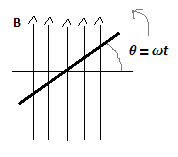
\includegraphics{flux.png}
\caption{\label VVoltage generator (side view)}
\end{figure}
\\
Let the area enclosed by the coil be $A$, the angular frequency of
rotation be $\omega$ such that $\theta = \omega t$, and the value of the
constant magnetic field be $B$. Now, by Faraday's law, the electric field $\mathcal{E}$ is defined as
\[ \mathcal{E}= - \frac{\partial \Phi_B}{\partial t} \]
where the flux $\Phi_B$ in this case is given by
\[ \Phi_B = BA \cos \theta = BA \cos \omega t \]
Hence the electric field will be
\[ \mathcal{E}= - BA \ \omega \sin \omega t \]
This is the principle of generation of the voltage supply that we receive at
our residences. This is one important reason why the sinusoidal voltage is
highly favoured and deeply studied. And of course there are many other reasons
why. Let us have a look at some interesting properties of sinusoids.
%%%
%%%
\subsection{Properties of sinusoids}
The first interesting thing about sine waves is that when you add two sinusoids
of the same frequency, it gives you back another sinusoid of the \emph{same}
frequency. Let's prove this formally.
Say we have two sinusoids, $x_1 (t)$ and $x_2 (t)$, of the same angular frequency
$\Omega,$ given by
\begin{equation*}
x_1 (t) = A_1 \cos (\Omega t + \phi_1)
\end{equation*}
\begin{equation*}
x_2 (t) = A_2 \cos (\Omega t + \phi_2)
\end{equation*}
Now consider a linear combination of the two sinusoids,
\begin{equation*}
x (t) = \alpha_1 x_1 (t) + \alpha_2 x_2 (t)
\end{equation*}
Note that we can write $x_1$ and $x_2$ as
\begin{equation*}
x_1 (t) = A_1  \{ \cos \Omega t \cos \phi_1 - \sin \Omega t \sin \phi_1 \}
\end{equation*}
\begin{equation*}
x_2 (t) = A_2  \{ \cos \Omega t \cos \phi_2 - \sin \Omega t \sin \phi_2 \}
\end{equation*}
Hence we can write $x (t)$ as
\begin{equation*}
x (t) = [ \alpha_1 A_1 \cos \phi_1 + \alpha_2 A_2 \cos \phi_2 ] \cos
   \Omega t + [ - \alpha_1 A_1 \sin \phi_1 - \alpha_2 A_2 \sin
   \phi_2 ] \sin \Omega t
\end{equation*}
Writing the two time-independent coefficients as $P$ and $Q$, we get
\begin{equation*}
 x (t) = P \cos \Omega t + Q \sin \Omega t = \sqrt{P^2 + Q^2}  \left\{
   \frac{P}{\sqrt{P^2 + Q^2}} \cos \Omega t + \frac{Q}{\sqrt{P^2 + Q^2}}
   \sin \Omega t \right\}
\end{equation*}
This can be easily seen to be
\begin{equation*}
 x (t) = \sqrt{P^2 + Q^2} \cos (\Omega t + \Phi)
\end{equation*}
with
\begin{equation*}
\Phi = - \tan^{- 1} \left( \frac{Q}{P} \right)
\end{equation*}
Hence, linearly combining two sinusoids of the same frequency gives back a
sinusoid with the same frequency.\\
Another interesting property is that when we differentiate a
sine wave, we get back a sinusoid of the same frequency.
\begin{equation*}
\frac{d}{d t}  \{ A \cos (\Omega t + \phi) \} = - A \Omega \sin
   (\Omega t + \phi)
\end{equation*}
It doesn't matter whether it is cosine or sine since they differ only by a
phase of $\pi / 2$.
\[ \cos (\Omega t + \phi) = \sin (\Omega t + \phi + \pi / 2) \]
Now let's see how we can describe a change in amplitude of a sinusoid.
Suppose the original sinusoid is given by
\[ x_1 (t) = A \cos (\Omega t + \phi) \]
and let the changed sinusoid is given by
\[ x_2 (t) = B \cos (\Omega t + \phi) \]
where $A$ and $B$ are positive constants. Then,
\[ x_2 (t) = \frac{B}{A} x_1 (t) \]
So the change of amplitude in a sinusoid is simply described by a multiplying
constant.\\
But this is not true for a phase change. Suppose the original sinusoid is
given by
\[ x_1 (t) = A \cos (\Omega t + \phi_1) \]
and the changed sinusoid is given by
\[ x_2 (t) = A \cos (\Omega t + \phi_2) \]
Unlike the amplitude case, $x_2 (t) / x_1 (t)$ doesn't turn out to be a
constant independent of time. This will cause a problem while dealing with
inductors or capacitors. In inductors, for example, the voltage drop is
proportional to the derivative of the current passing through it. Hence, if a
sinusoidal current is passing through it, the voltage drop across it will also
be a sinusoid, but will have a phase difference of $90^0$ with the current.
Hence, we cannot establish a relationship like the resistor $(V = RI)$ in case
of the inductor since $V / I$ won't be a constant independent of time.\\
To deal with this problem, we will have to use the rotating complex number
representation of the sinusoid.

\subsection{Sinusoids as Rotating Complex Numbers}

We can think of a sinusoid $I_0 \cos (\Omega t + \phi_0)$ as a combination of
two rotating complex numbers. Let the first begin at time $t = 0$ with an
angle of $\phi_0$. Let it have a magnitude of $I_0 / 2$ and let the other
begin with the same magnitude $I_0 / 2$ but the opposite starting angle ($-
\phi_0$). Let them both rotate with an angular velocity of $\Omega$, but the
first one in counter clockwise and the second one in clockwise direction.
\begin{figure}[ht]
\centering
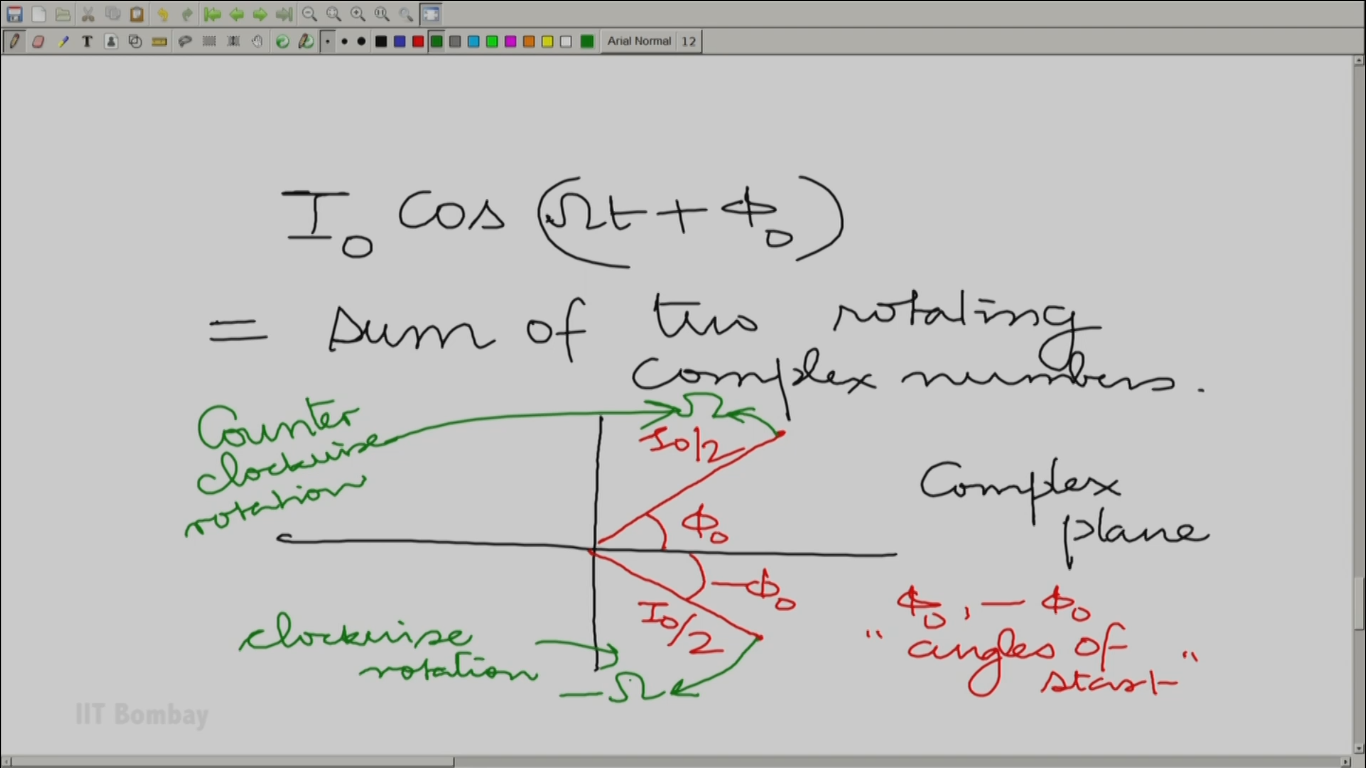
\includegraphics[scale=0.28]{rotating_complex.png}
\end{figure}
\\
We can express these two complex numbers in the polar form as
\[ c_1 = \frac{I_0}{2} e^{j \{ \Omega t + \phi_0 \}} \]
\[ c_2 = \frac{I_0}{2} e^{- j \{ \Omega t + \phi_0 \}} \]
where $j = \sqrt{- 1}$. One can see that $c_1 + c_2$ gives back the original
sinusoid.\\
It seems like a silly thing to do to describe a sinusoid as a combination of
two rotating complex numbers. But the reason for doing this is clear when we
look at the inductor once again.\\
Let's assume for now that we provide to the inductor, an input which is just
one of those rotating complex numbers. So
\[ I = \frac{I_0}{2} e^{j \{ \Omega t + \phi_0 \}} \]
Now, the voltage across an inductor is given by
\[ V = L \frac{d I}{d t} = L\frac{I_0}{2} (j \Omega) e^{j \{ \Omega t +
   \phi_0 \}} \]
Hence we can see that
\[ V / I = j \Omega L \]
Now the ratio of the voltage and current for an inductor is a complex
\textit{constant independent of time}!\\
Similarly, for the other rotating complex number, we will get $V / I$ again to
be a constant, but with a minus sign $(- j \Omega L)$. So in some sense the
actual angular frequency, whether positive or negative, is reflected. It is left as an exercise to do a similar analysis for capacitances and verify that
for capacitors,
\[ V / I = \frac{1}{j \Omega C} \]
This makes the analysis of RLC circuits (circuits consisting of Resistor(s),
Inductor(s) and Capacitors(s)) much easier as we can interpret these constants
as generalised resistances, or \textit{impedances.} In that sense, the
resistor has an impedance of $R$, an inductor has an inductance of $j \Omega
L$ and a capacitor has an impedance of $1 / j \Omega C$.\\
Notice that $c_1$ and $c_2$ defined above are complex conjugates of each
other. So whatever happens to $c_1$ is mirrored in $c_2$. For example, the $V
/ I$ for $c_2$ ($- j \Omega L$) is the complex conjugate of the $V / I$ for
$c_1$ ($j \Omega L$).\\
The analysis of sinusoids using rotating complex numbers is known as `phasor'
analysis. As the rotating complex numbers are constant in magnitude, but
change their phase, they are called `phasors'.\\
This is the reason why we earlier demanded that our systems should accept a
complex signal in general.\\
In a nutshell, dealing with amplitudes is easy but the dealing with phases is
a problem in sinusoids and that problem is overcame when you go to the phasor
instead of the corresponding sinusoid. Let us see how a general LSI system responds to
a phasor or sinusoid as an input.
\section{Module 2: Lecture 2\\Sinusoidal Input to LSI Systems}


%\subsection{Introduction}

\subsection{Understanding Phase Change In Sinusoids and Phasors}
We write a sinusoid as a combination of two rotating complex numbers, which we will henceforth call phasors, moving in opposite directions. 
\[
	2Acos(\Omega t + \phi) = Ae^{j(\Omega t + \phi)} + Ae^{-j(\Omega t + \phi)}
\]
Let us focus our attention on one of the phasors for now. Let us look at what happens when we introduce a phase change.\\
\[
Ae^{j(\Omega t + \phi)} \xrightarrow{Phase \ Change} Ae^{j(\Omega t + \phi + \Delta\phi)}
\]
\[
Ae^{j(\Omega t + \phi + \Delta\phi)} =
Ae^{j(\Omega t + \phi)}e^{j\Delta\phi}
\]
We hence find that a change of phase results just in a multiplying factor which is a constant independent of time.\\
Now we try to do a similar calculation for the complex conjugate (the phasor moving in the opposite direction).
\[
Ae^{-j(\Omega t + \phi)} \xrightarrow{Phase \ Change} Ae^{-j(\Omega t + \phi)}e^{-j\Delta\phi}
\]
Notice that the multiplying constant in this case is the complex conjugate of the previous multiplying factor we found.\\
\[
	2Acos(\Omega t + \phi) \xrightarrow{Phase \ Change} Ae^{j(\Omega t + \phi)}e^{j\Delta\phi} + Ae^{-j(\Omega t + \phi)}e^{-j\Delta\phi}
\]
We hence understand that using only one phasor is enough to fully determine the behaviour of the sinusoid. This explains why we used complex signals in our previous analysis, due to their ease in mathematical manipulation.\\
We will now see the result of inputting a sinusoidal signal to a stable linear shift invariant system, with impulse response $h(t)$ (Assume that the impulse response is real). We deal with stable LSI systems because the output will be bounded.\\
\begin{figure}[ht]
\begin{center}
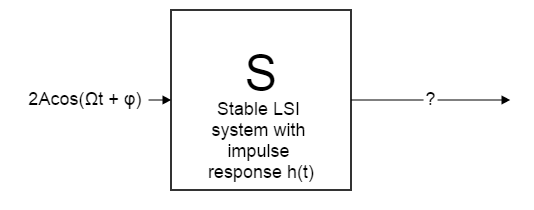
\includegraphics[width=10cm]{LSIcos.png}
\caption{Sinusoidal Input To Stable LSI System}
\end{center}
\end{figure}
The output for an LSI system is given by the convolution of the input and the impulse response.
The direct solution via convolution seems very difficult. In fact if we try to calculate the convolution integral, we get the following expression:
\[
y(t) = \int_{-\infty}^{+\infty} \! {h(\lambda)2Acos(\Omega(t-\lambda) + \phi) \ \dm \lambda}\]
We will now see how to solve it using phasors, making the analysis mathematically convenient.
%%%
%%%
\subsection{Phasor Input to LSI System}
Consider the output when a phasor is input to a stable LSI system.
\[
Ae^{j(\Omega t + \phi)} \xrightarrow{LSI} 
 \int_{\infty}^{\infty} \! Ae^{j(\Omega (t - \lambda) + \phi)}h(\lambda) \ \dm \lambda
\]
 
\[ =
Ae^{j(\Omega t + \phi)} \int_{\infty}^{\infty} \! {e^{-j\Omega\lambda}h(\lambda) \ \dm \lambda}
\]
Here, we see that we get the output to be the input phasor with a multiplying factor $\int_{-\infty}^{\infty} \! {e^{-j\Omega\lambda}h(\lambda) \ \dm \lambda}$, which is dependent only on $\Omega$ and $h$ (it is constant with respect to time).\\
We will now come back to the importance of why we chose our system to be stable. We will do this by trying to find a bound to the absolute value of the multiplying factor we just found.
\[
| \int_{-\infty}^{\infty} \! {e^{-j\Omega\lambda}h(\lambda) \ \dm \lambda} | \leq 
\int_{-\infty}^{\infty} \! { |e^{-j\Omega\lambda}||h(\lambda)| \ \dm \lambda }
\]
\[
\int_{-\infty}^{\infty} \! { |e^{-j\Omega\lambda}||h(\lambda)| \ \dm \lambda } =
\int_{-\infty}^{\infty} \! {|h(\lambda)| \ \dm \lambda }
\]
And as per the condition of stability the integral of the absolute value of the impulse response is bounded. Hence the absolute value of the multiplying factor is also bounded. In fact we have obtained a concrete bound to this integral, namely the absolute integral of the impulse response. We can do similar mathematical analysis for the conjugate as well.\\
This multiplying factor is called the \textit{Frequency Response} of the LSI system at angular frequency $\Omega$.
\[
	Frequency\ Response\ H(\Omega) = \int_{-\infty}^{\infty} \! {e^{-j\Omega\lambda}h(\lambda) \ \dm \lambda}
\] 
%%%
%%%
\subsection{Sinusoid Input to LSI System}
We will now come back to our original problem of inputting a sinusoidal signal into a stable linear shift invariant system. We will begin by simplifying the outputs of the two phasors.
\[
	H(\Omega)Ae^{j(\Omega t + \phi)} = |H(\Omega)|Ae^{j(\Omega t + \phi +  \angle  H(\Omega))}
\]
The complex conjugate of the frequency response is given by
\[
\bar{H}(\Omega) = \int_{-\infty}^{\infty} \! {e^{j\Omega\lambda}h(\lambda) \ \dm \lambda} = H(-\Omega)
\]
Note that the first equality holds only if $h(\lambda)$ is real.
Hence,
\[
H(-\Omega)Ae^{-j(\Omega t + \phi)} = |H(\Omega)|Ae^{-j(\Omega t + \phi +  \angle  H(\Omega))}
\]
So we can check by adding the two outputs that the output for inputting a sinusoid $2Acos(\Omega t + \phi)$ is given by:

\[
2Acos(\Omega t + \phi) \xrightarrow{Stable\ LSI} 2A|H(\Omega)|cos(\Omega t + \phi + \angle H(\Omega))
\]
This indicates that on passing through a stable LSI system, a sinusoid goes through an amplitude and phase shift which is independent of time and only dependent on the impulse response and angular frequency of the sinusoid. Note again that the impulse response has to be real for this to hold true.\\
Also, if we view an input to a stable LSI system as the sum of multiple sinusoids, the output can be visualized as the sum of the corresponding outputs of the sinusoids through the stable LSI system. The stability of the LSI systems guarantees the existence of the frequency response of the system. But if it is unstable it may or may not have a frequency response.
%%%
%%%
\subsection{Periodic Input to Shift Invariant Systems}
How does an LSI system respond to a general periodic signal? Consider the following lemma.\\
\textbf{Lemma:} A periodic input to a shift invariant system produces a periodic output.\\
\textbf{Proof:}\\
%%%
Let the input be $x(t)$ with a period $T$
\[x(t+T) = x(t)\ \ \forall t\]
\[x(t) \xrightarrow{SI\ system} y(t) \]
%%%
Now, by shift invariance,
\[x(t+T) \xrightarrow{SI\ system} y(t+T) \]
Hence,
\begin{equation}\label{eqn:PeriodicOutput}
y(t) = y(t+T)\ \ \forall \ t
\end{equation}
Hence the output is also periodic, infact with the same period $T$.\\
An important property of a periodic input or a periodic function is that it can be represented by a linear combination (which can be countably infinite) of sinusoids having frequencies which are multiples of the frequency of the input. This property is referred to as the existence of a Fourier Series expansion of the input. \\
The Fourier Series expansion and our understanding from the previous section gives us a simple method to compute the output of a periodic input in an LSI system as the linear combination of the output of these sinusoids.\\
%% Added paragraph for better flow. Needs verification:
This result, combined with \ref{eqn:PeriodicOutput} can be used to calculate the output for a general periodic input, but for that, we need still more information. How do we know whether a certain periodic signal can be expressed as a linear combination of sinusoids \emph{uniquely}? To answer this question, we need to invoke some concepts from linear algebra by considering signals as vectors.

%\subsection{Conclusion}
%In this lecture we understood the analysis of inputting sinusoidal input to a stable LSI system. We saw how we could simplify our analysis by the use of phasors. In the upcoming lecture we will learn about the use of inner product and vector analysis in understanding signals.


\section{Module 2: Lecture 3\\Signals and Vectors}

\subsection{Introduction}
In the previous lecture, we have learnt how a periodic input given to a Linear Shift Invariant system results in a periodic output with the same period. Now in this lecture we will see some new concepts by which every input can be expressed as sinusoidal inputs. Henceforth, it will be simpler to analyse their outputs.

\subsection{Relations between Signals and Vectors}
\label{sec:examples}
Consider a 2-dimensional vector, we can decompose this vector into two perpendicular components with $e_1$ and $e_2$ as the unit vectors along those directions. To find these components, we need to use Dot Product.
\subsubsection{Dot Product}
	Dot Product of two vectors u and v is defined as the magnitude of vector u multiplied by the magnitude of v multiplied by cosine of the angle between these two vectors.
    
	    					\begin{equation*}u.v = |u||v|cos\theta\end{equation*}
                            
where $\theta$ is the angle between vectors u and v. If u is a unit vector, then the dot product of vectors v and u gives the component of vector v in the direction of u, with the value |v|cos$\theta$.
	\begin{figure}[ht]
\centering
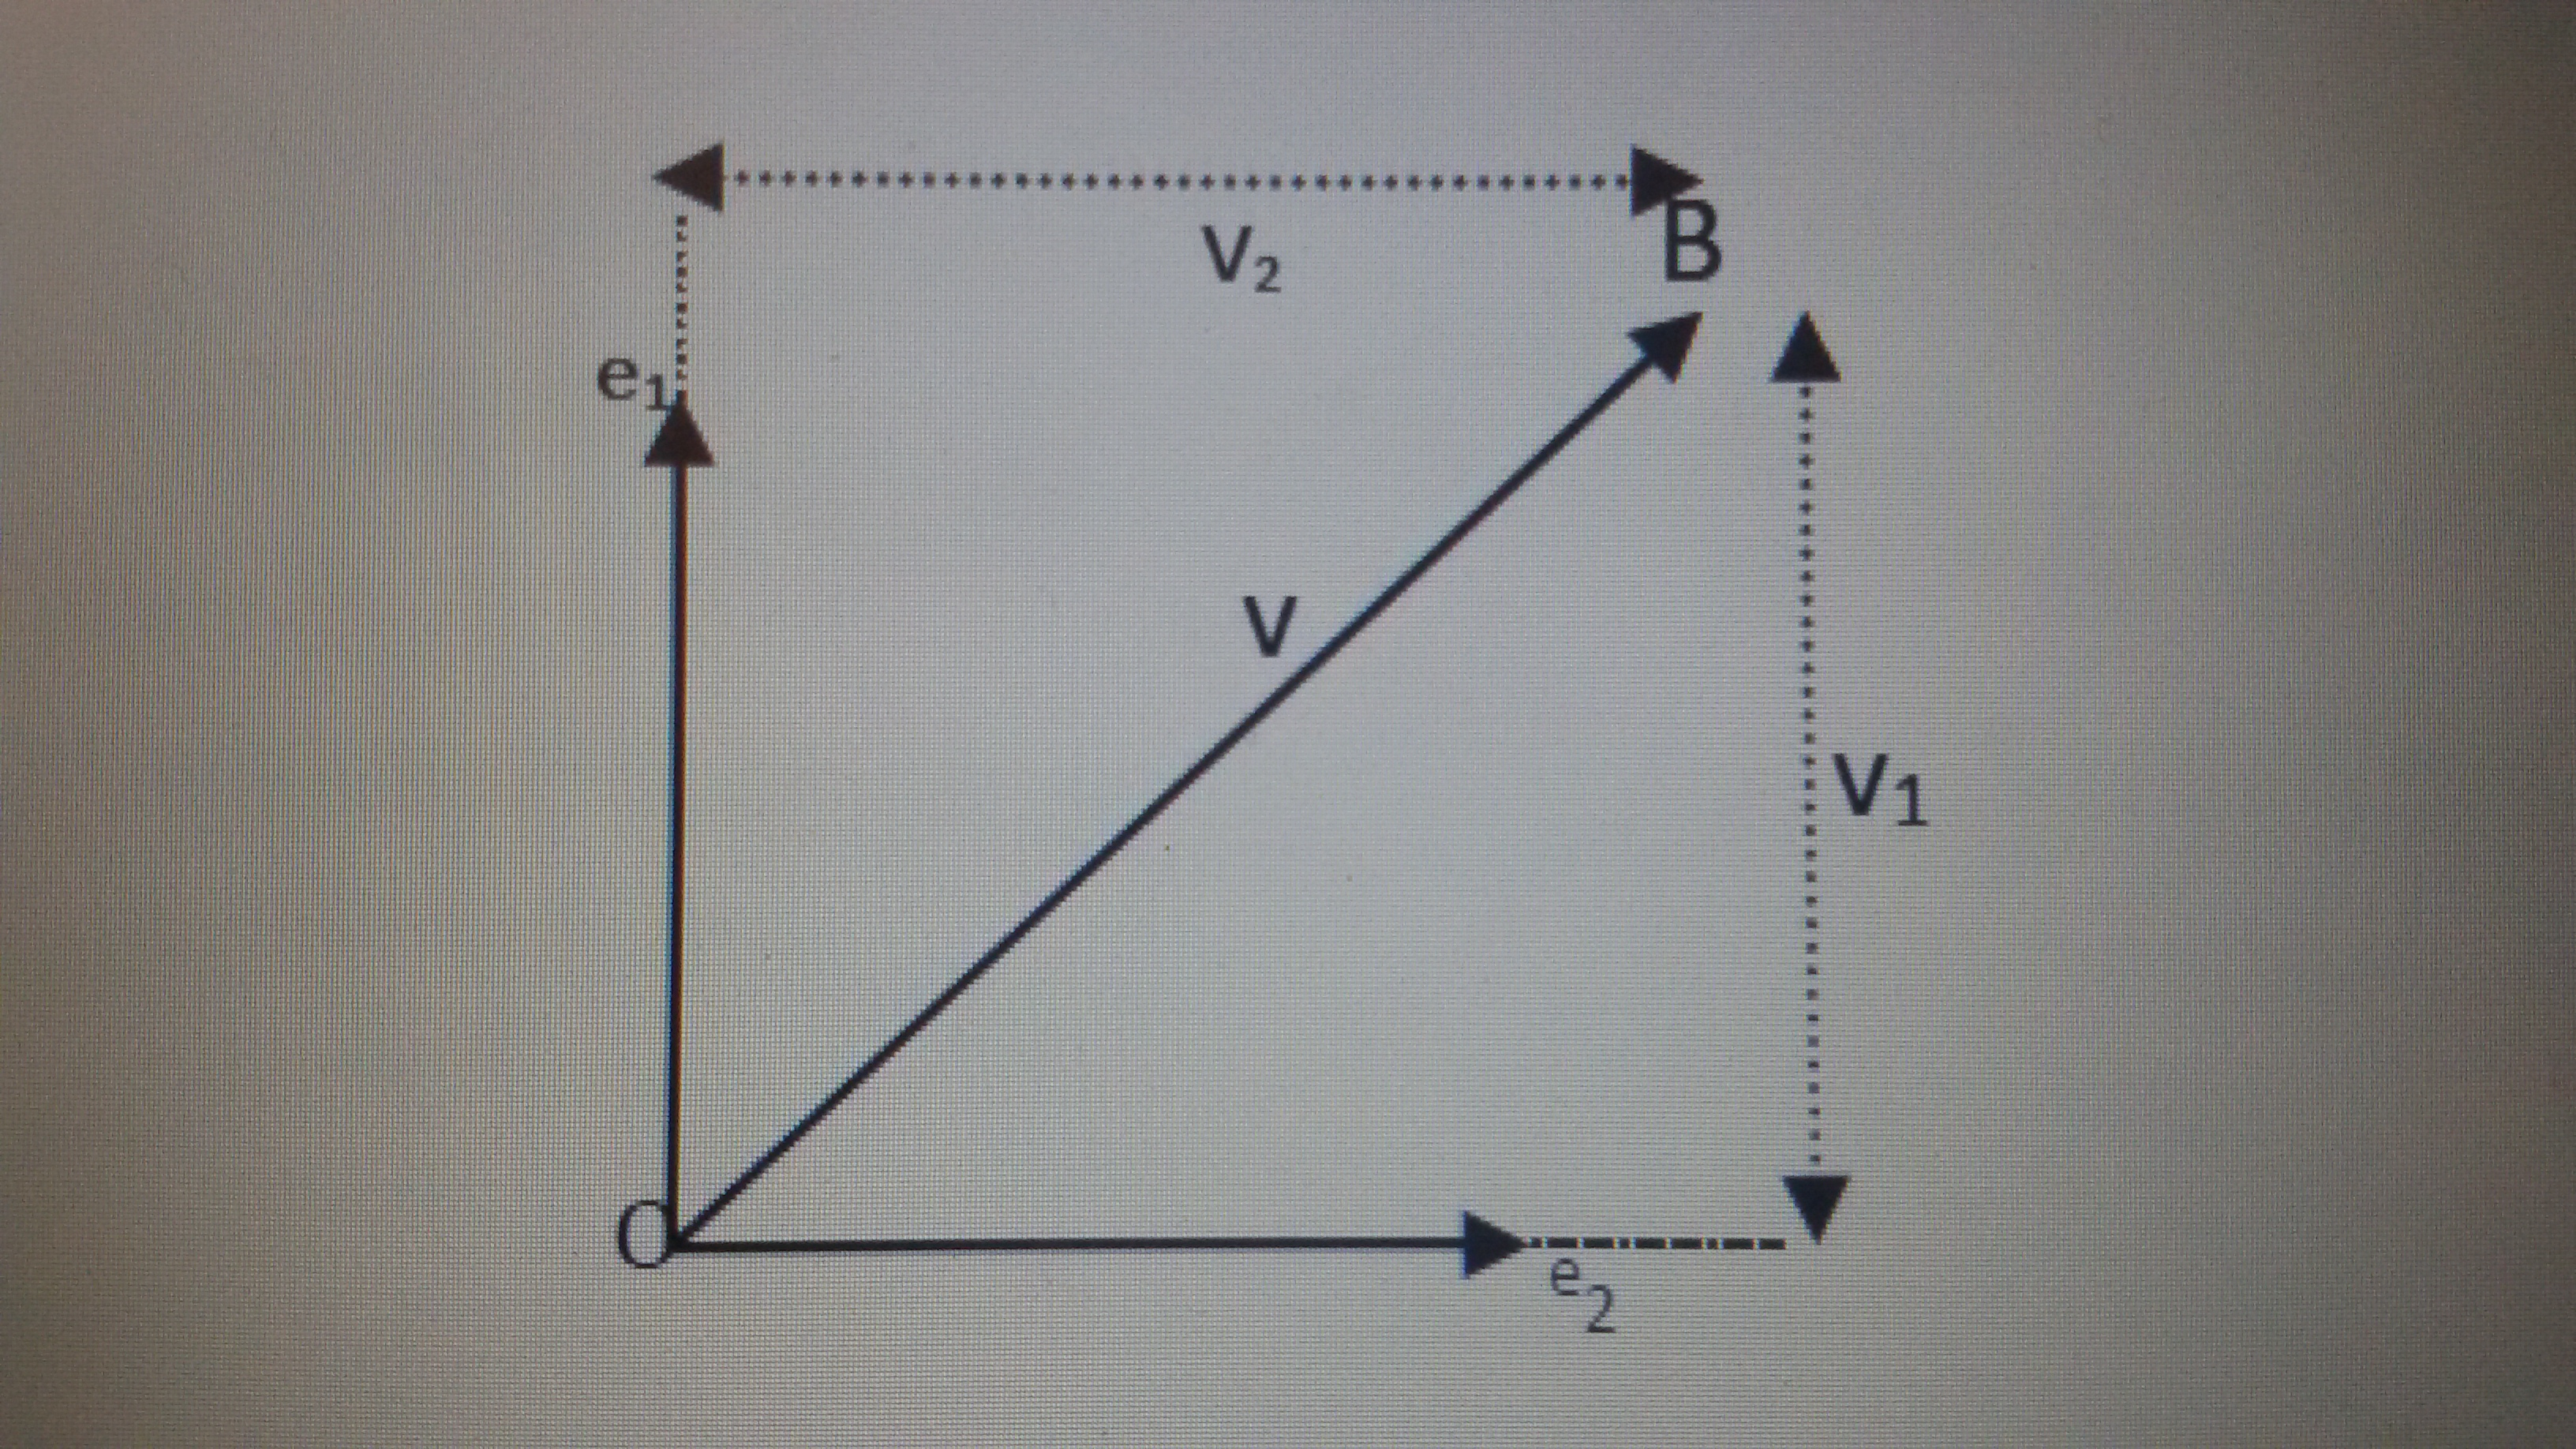
\includegraphics[scale=0.08]{figure.jpg}
\end{figure}
    
    
    Consider the above figure, here OB is a vector denoted by v which is expressed as
    \begin{equation*}v = v_1e_1 + v_2e_2\end{equation*}
    
    where $v_1$ and $v_2$ are the components in $e_1$ and $e_2$ directions respectively.
By this we can say that vectors $e_1$ and $e_2$ spans the space in 2D i.e. we can express any vector as a linear combination of e1 and e2. A collection of vectors span a space. Suppose if any vector can be expressed uniquely as a linear combination of $\{ u_1$,$u_2$,$u_3$ .... $u_n \}$, where $\{ u_1$,$u_2$,$u_3$...$u_n \}$ are linearly independent, then $\{ u_1$,$u_2$...$u_n \}$ is said to form a basis.\\
\noindent
Also, if $\langle u_i$,$u_j \rangle$ = 0 for i,j belonging from 1 to n,i.e. dot product of any two vectors is zero,  then the basis is said to be an \textit{orthogonal basis}. Finally, for a n-dimensional space, a collection of n linearly independent vectors forms the basis.\\
\noindent
The dot product of two vectors $u$ and $v$ is equal to the sum of the products of the corresponding perpendicular components. Suppose

				\begin{equation*}u = u_1e_1 + u_2e_2\end{equation*}
                        
                        \begin{equation*}v = v_1e_1 + v_2e_2\end{equation*} 
\noindent                        
                        therefore,\begin{equation*} u.v = u_1v_1 + u_2v_2\end{equation*}
           
\subsubsection{Dot Product of Discrete Sequences}           
Now, consider a discrete sequence with 2 non-zero points. This sequence can be compared to a 2-dimensional vector v with $v_1$ and $v_2$ as its perpendicular components such that it is equal to the values at the 2 non zero points of the sequence. Similarly for a sequence with n non-zero points can be considered as a vector in n dimensional space. Also, the concept of dot product is similarly applied to the discrete sequences.

For example : Consider
	x[n] = $(1/2)^n$ u[n];
    
    i.e.
     \begin{equation*}
    x[n] = (1/2)^n	\enspace	\enspace for\enspace	 n\geq0\end{equation*}
    \begin{equation*}	 0	\enspace  \enspace	 for\enspace	 n<0\end{equation*}
               
	 \begin{equation*} y[n] = (1/3)^nu[n] \end{equation*}
    
    i.e. 
    \begin{equation*}y[n] = (1/3)^n	\enspace \enspace	for\enspace n\geq0\end{equation*} \begin{equation*}0\enspace \enspace			for\enspace n<0 \end{equation*}
                  
                  
  Lets calculate the dot product of x[n] and y[n],i.e. summing the product of corresponding components.
  We have,
   \begin{equation*} \langle x[n],y[n] \rangle = \sum_{n=-\infty}^{\infty}\ x[n]y[n]\end{equation*} 
   \begin{equation*} \langle x[n],y[n] \rangle = \sum_{n=0}^{\infty}\ x[n]y[n]\end{equation*} 
   \begin{equation*} \langle x[n],y[n] \rangle = \sum_{n=0}^{\infty}\ (1/2)^n*(1/3)^n\end{equation*} 
   \begin{equation*} \langle x[n],y[n] \rangle = \sum_{n=0}^{\infty}\ (1/6)^n\end{equation*} 
   \begin{equation*} \langle x[n],y[n] \rangle = \frac{1}{(1-(1/6))}\end{equation*} 
   \begin{equation*} \langle x[n],y[n] \rangle = \frac{6}{5}\end{equation*} 
  		
          
 	By this we compute the dot product of two discrete sequences. This dot product is also called as \textit{Inner Product}. Inner product of two vectors $u$ and $v$ is represented by $\langle u,v \rangle$.

\subsubsection{Inner Product of Continuous Signals}
       In a discrete sequence, a unit vector can be expressed as $\delta[n-N]$ for all integers Z. A n-dimensional vector v can be expressed as
        \begin{equation*}v = v_1e_1 + v_2e_2 + ........ + v_ne_n\end{equation*}
        Now writing the above equation in terms of sequences, we have
       
    	\begin{equation*}	x[n] = 	\sum_{n=-\infty}^{\infty}\ x[N]\delta[n-N]\end{equation*}
            
            where x[n] is the component along dimension N.
       
Similarly applying the same concept for continuous time functions, we need to replace summation by integral, which gives,

					\begin{equation*}x(t) = \int_{-\infty}^{\infty} \! x(\lambda)\delta[t-\lambda] \ \mathrm{d}\lambda\end{equation*}
                    
             where x($\lambda$) is the component in direction $\lambda$ and $\delta[t-\lambda]$ is continuous impulse at $\lambda$ similar to unit vector.So inner product of x(t) and y(t) is given by
             
           \begin{equation*} \langle x(t),y(t) \rangle = \int_{-\infty}^{\infty} \! x(t)y(t) \ \mathrm{d} t\end{equation*}
             
 \subsection{Sinusoids with same period}
          Let us see how we can express any signal as sinusoidal functions. So, first we need to find sinusoidal signals which are perpendicular. Consider a signal x(t) which is periodic with period T,i.e. \begin{equation*}  x(t) = x(t+T)\end{equation*}. Assume that it can be expressed as a sum of sinusoidal functions. We should take a sinusoidal function which is periodic with period T. So it is of the form $A_k\cos (\frac{2\pi}{T}kt + \phi_k)$. We have,
          
          \begin{equation*}x(t) = \sum_{k=-\infty}^{\infty}\ A_k\cos (\frac{2\pi}{T}kt + \phi_k)\end{equation*}
          
          Let's take two different \textit{k}
.  \begin{equation*}
x_1 (t) = A_1 \cos (\frac{2\pi}{T}k_1t + \phi_1)
\end{equation*}
           and \begin{equation*}
x_2 (t) = A_2 \cos (\frac{2\pi}{T}k_2t + \phi_2)
\end{equation*}
          Consider the inner product of $x_1(t)$ and $x_2(t)$ with the interval going from 0 to T. We are here restricting our interval to T because the integral might diverge when we integrate from 0 to $\infty$. We have,
           \begin{equation*}\langle x_1(t),x_2(t) \rangle = \int_{0}^{T} \! x_1(t)x_2(t) \ \mathrm{d}t\end{equation*}
           \begin{equation*}\langle x_1 (t),x_2 (t) \rangle = \int_{0}^{T} \! \cos (\frac{2\pi}{T}k_1t + \phi_1) \cos (\frac{2\pi}{T}k_2t + \phi_2) \ \mathrm{d}t\end{equation*}
           Using 
          \begin{equation*} 2cosAcosB = cos(\frac{A+B}{2}) + cos(\frac{A-B}{2})\end{equation*}
          We have,
          \begin{equation*}\langle x_1 (t),x_2 (t) \rangle = \int_{0}^{T} \! \left\lbrace \cos (\frac{2\pi}{T}\frac{(k_1+k_2)}{2}t + \frac{\phi_1+\phi_2}{2}) + \cos (\frac{2\pi}{T}\frac{(k_1-k_2)}{2}t + \frac{\phi_1-\phi_2}{2}) \right\rbrace \ \mathrm{d}t \end{equation*}
          
          
        
        
                
                If ($k_1$ + $k_2$) or ($k_1$ - $k_2$) are not zero, that means we have a finite number of cycles of the sinusoids, implying the integral is zero. However if $k_1$=$k_2$, the second integral becomes T times $\cos (\theta_1-\theta_2)$.
                Thus we have,
            \begin{equation*} \langle x_1 (t),x_2 (t) \rangle  \neq 0	\enspace \enspace		for \enspace k_1 = k_2\end{equation*}
            \begin{equation*} \langle x_1 (t),x_2 (t) \rangle = 0	\enspace \enspace		for \enspace k_1 \neq k_2\end{equation*}
                
                
                Hence, we have proved that two sinusoids with same time period are perpendicular if they don't have same angular frequency and vice-versa. Thus using this important concept, we will be able to write any signal as sum of sinusoidal signals and hence analysis of these signals will be simpler.


\section{Module 2: Lecture 4\\Decomposition of Signals}

\subsection{Introduction}
\noindent
 A fundamental idea in the study of signals is to represent signals in terms of linear combination of \textit{basis} signals. In the previous section, we have embarked on some important concepts, relating to the idea of representing signals as a linear combination of sinusoids.
 %In this lecture, we will be recapitulating those ideas.
We assumed that we wish to look either at periodic signals or signals over a finite interval $T$. Without loss of generality, let that interval be $(0,T)$. 

\noindent
We have assumed that such signals are signals spanned by  all sinusoids of angular frequency $\Omega = \frac{2\pi}{T}kt,k=0, \pm1, \pm2 ..$

\noindent
The typical periodic function, with period $T$ is of the form
\begin{equation*}
  x(t) = \sum_{k=-\infty}^{\infty} \! A_k\cos (\frac{2\pi}{T}kt + \phi_k)
\end{equation*}
where $A_k$ denotes the amplitude, $\Omega = \frac{2\pi}{T}k$ is the angular frequency and $\phi_k$ the phase.
We had proved that these sinusoids are orthogonal if they don’t have same angular frequency.
\begin{equation*}
  \langle A_{k_1} \cos (\frac{2\pi}{T}k_1t + \phi_1),A_{k_2} \cos (\frac{2\pi}{T}k_2t + \phi_2)\rangle = 0 \enspace \enspace \text{for} \enspace k_1 \neq k_2 
\end{equation*}

\noindent
This important concept requires appreciating several different ideas. Using these ideas, we can decompose signal $x(t)$ in terms of sinusoids. However, there are some signals which can’t be spanned using these sinusoids. Such signals are beyond the scope of discussion that we are going to undertake at this stage.
%%%
%%%
\subsection{ Orthogonal vectors at a particular frequency}
\noindent
Consider a periodic signal $x(t)$ with fundamental period $T$. Then we can write $x(t)$ as
%Let us assume the signal $x(t)$ as
\begin{equation*}
  x(t) = \sum_{k=-\infty}^{\infty} \! A_k\cos (\frac{2\pi}{T}kt + \phi_k)
\end{equation*}
%where $x(t)$ is periodic with period $T$ and w
We constrain ourselves to $0<t<T$.

\noindent
To calculate $A_k$ and $\phi_k$ we need to use the following property i.e.
\begin{equation*}
\langle \cos (\frac{2\pi}{T}k_1t + \phi_1), \cos (\frac{2\pi}{T}k_2t + \phi_2) \rangle = 0 \enspace \enspace		for \enspace k_1 \neq k_2 \end{equation*}

\noindent
We can think of the cosines $\cos (\frac{2\pi}{T}kt + \phi_k)$ as countably infinite orthogonal vectors, indexed by $k$, for $k=0, \pm1, \pm2...$ and so on.

\noindent
To find out the component of $x(t)$ along these orthogonal vectors, we need to take the dot product of $x(t)$ with the unit vector, in the direction of orthogonal vectors $\cos(\frac{2\pi}{T}kt + \phi_k), 0<t<T$.
For calculating unit vector, we need to find the magnitude of the vector $\cos(\frac{2\pi}{T}kt + \phi_k)$ using dot product.

\begin{align*} \left|\cos(\frac{2\pi}{T}kt + \phi_k)\right| &= \langle \cos (\frac{2\pi}{T}kt + \phi_k), \cos (\frac{2\pi}{T}kt + \phi_k)\rangle \\
  &= \int_{0}^{T} \! \cos (\frac{2\pi}{T}kt + \phi_k) \cos (\frac{2\pi}{T}kt + \phi_k) \ \dm t \\
  &= \int_{0}^{T} \! \cos^2 (\frac{2\pi}{T}kt + \phi_k) \ \dm t \\
  &= \int_{0}^{T} \! (\frac{1}{2} + \cos (2(\frac{2\pi}{T}kt + \phi_k)) \ \dm t \\
  &= \int_{0}^{T} \! \frac{1}{2} \ \dm t + \int_{0}^{T} \! \cos (2(\frac{2\pi}{T}kt + \phi_k)) \ \dm t \\
  &= \frac{T}{2}
\end{align*}
%%%
Thus, the magnitude square of the cosine is $T/2$ and hence the magnitude is $\sqrt{T/2}$. So, the unit vector is given by

\begin{equation*} \textrm{Unit vector} = \sqrt{\frac{2}{T}}\cos (\frac{2\pi}{T}kt + \phi_k)\end{equation*}
                    
\noindent
But still, there is one unknown quantity, namely, $\phi_k$ in this unit vector. However, we can think of this vector as a vector in a two dimensional space:

\begin{equation*}\sqrt{\frac{2}{T}}\cos (\frac{2\pi}{T}kt + \phi_k) = \sqrt{\frac{2}{T}}[\cos\phi_k\cos (\frac{2\pi}{T}kt) - \sin\phi_k\sin (\frac{2\pi}{T}kt)] \end{equation*}
that is, the unit vector can be thought of as a linear combination of two vectors.

\noindent
We have,
\begin{align*}
  \langle \cos (\frac{2\pi}{T}kt + \phi_k), \sin (\frac{2\pi}{T}kt + \phi_k) \rangle &= \int_{0}^{T} \! \cos (\frac{2\pi}{T}kt + \phi_k) \sin (\frac{2\pi}{T}kt + \phi_k) \ \dm t  \\
  &= \frac{1}{2} \int_{0}^{T} \! 2 \cos (\frac{2\pi}{T}kt + \phi_k) \sin (\frac{2\pi}{T}kt + \phi_k) \ \dm t \\
  &= \frac{1}{2} \int_{0}^{T} \! \sin (\frac{4\pi}{T}kt + \phi_k) \ \dm t \\
  &= 0
\end{align*}
%%%
Hence, the cosine and sine components are also orthogonal. $\cos\phi_k$ and $\sin\phi_k$ are now two unknown constants.
%%%
Therefore, decomposing $x(t)$ along $\cos (\frac{2\pi}{T}kt + \phi_k)$ will give the same results as decomposing $x(t)$ along  $\cos (\frac{2\pi}{T}kt)$ and $\sin (\frac{2\pi}{T}kt)$. So, to decompose $x(t)$ along $\cos (\frac{2\pi}{T}kt)$ and $\sin (\frac{2\pi}{T}kt)$, we require unit vectors, which we already have calculated above.
%%%
So, the two unit vectors are $\sqrt{\frac{2}{T}}\cos (\frac{2\pi}{T}kt)$ and $\sqrt{\frac{2}{T}}\sin (\frac{2\pi}{T}kt)$.
%%%
%%% 
\subsection{Projection of Vectors}
Let $u_1$ = $\sqrt{\frac{2}{T}}\cos (\frac{2\pi}{T}kt)$ and $u_2 = \sqrt{\frac{2}{T}}\sin (\frac{2\pi}{T}kt)$. We know that at frequency $2\pi k/T$, there are two orthogonal vectors, $u_1$ and $u_2$. We have a two dimensional space and we need to calculate the component of the vector $x(t)$ along orthogonal vectors of this 2D space.
  
\noindent
 Let $v$ be any arbitrary vector of higher dimension and $v_p$ be the projection of $v$ onto our 2D space spanned by orthogonal vectors $u_1$ and $u_2$. To calculate the components of the vector $v$ along the two orthogonal vectors, we can project $v_p$  onto $u_1$ and $u_2$. We can also directly project $v$ onto $u_1$ and $u_2$.
 


\noindent
 The vector $v$ can be written as $v = v_p  + v_\perp$, where $v_p$ is the projection of $v$ on to 2D space and $v_\perp$ is component perpendicular to the 2D space . The projection of $v$ onto vectors $u_1$ and $u_2$ will be same as the projection of $v_p$  on those vectors, as the $v_\perp$ will not contribute in projection.
 
\begin{figure}[ht]
\centering
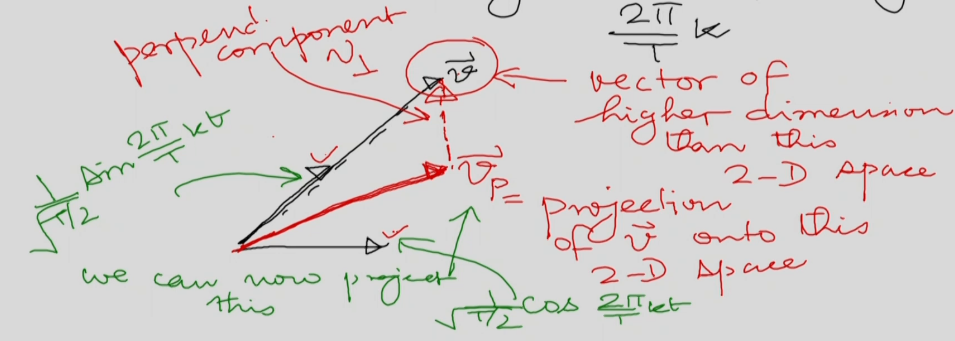
\includegraphics[scale=0.32]{S_215.PNG}		
\end{figure}

 \begin{figure}[ht]
\centering
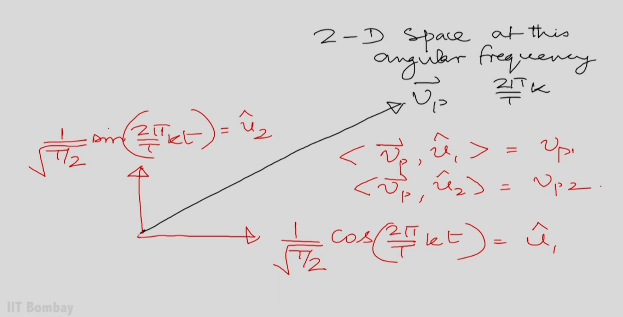
\includegraphics[scale=0.32]{S_215_2.PNG}		
\end{figure}

\noindent
Let us project $v_p$ along the two orthogonal vectors. 
  For projecting  $v_p$  along $u_1$ and $u_2$, taking dot product 
 
\begin{equation*} \langle v_p, u_1 \rangle =v_{p_1} \end{equation*}
\begin{equation*} \langle v_p, u_2 \rangle = v_{p_2} \end{equation*}
 
\noindent
$v_p$  in terms of $u_1$, $u_2$ can be written as $v_p$  = $v_{p_1}u_1$ + $v_{p_2}u_2$. Interestingly  $\langle v_p, u_1 \rangle = \langle v, u_1 \rangle$ is true also for $u_2$ as the perpendicular component $v_\perp$ is not going to contribute in the dot product. 
        
We know that the $k^{th}$ angular frequency =  $2 \pi k/T$.
At this frequency we have two components 
\begin{equation*}x(t) = \langle x(t), \sqrt{\frac{2}{T}}\cos (\frac{2\pi}{T}kt)\rangle \cdot \sqrt{\frac{2}{T}}\cos (\frac{2\pi}{T}kt) + \langle x(t), \sqrt{\frac{2}{T}}\sin (\frac{2\pi}{T}kt)\rangle \cdot \sqrt{\frac{2}{T}}\sin (\frac{2\pi}{T}kt)\end{equation*}
This can be simplified as

\begin{equation*}x(t) = \langle x(t), \cos (\frac{2\pi}{T}kt)\rangle \cdot \frac{2}{T}\cos (\frac{2\pi}{T}kt) + \langle x(t), \sin (\frac{2\pi}{T}kt)\rangle \cdot \frac{2}{T}\sin (\frac{2\pi}{T}kt)\end{equation*}

\noindent
\subsection{Decomposition of square wave}
We have a periodic signal $x(t)$ in Fig.\ref{fig:square-wave}, defined as
\[
x(t) =
\left\{
	\begin{array}{ll}
		1  & \mbox{if } 0 < t < \frac{T}{2} \\
		-1 & \mbox{if } \frac{T}{2} < t < T
	\end{array}
\right.
 \]

\noindent
$x(t) = x(t+T)$ for all $t$, i.e. $x(t)$ is periodic with period $T$.
              
\begin{figure}[ht]\label{fig:square-wave}
\centering
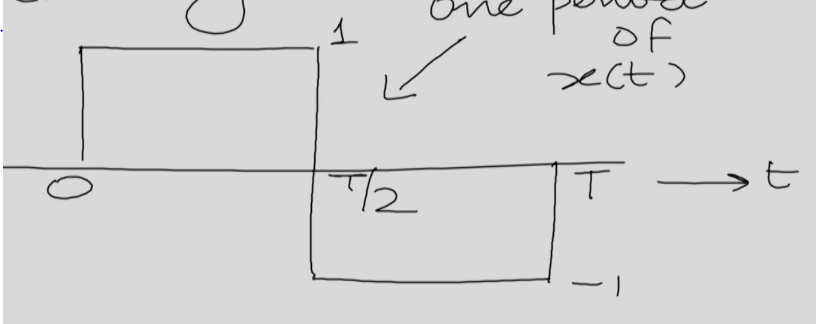
\includegraphics[scale=0.32]{S_216_1.PNG} %\\Figure 1
\caption{Plot of $x(t)$}
\end{figure}




\noindent
The zero frequency component is the  mean of $x(t)$ over a period $T$ which is $0$ since the net area under $x(t)$ in one period is zero.

\noindent
Let us calculate the quantity $\langle x(t), \cos (\frac{2\pi}{T}kt)\rangle \cdot \frac{2}{T}\cos (\frac{2\pi}{T}kt))$,


\noindent
For $k=1$ and $k=2$, we can see from Fig.\ref{fig:square-dot-cosine} that, the positive portion gets annulled by the negative portion. Similar is the case for $k=3, 4...$ and so on. Hence $\langle x(t), \cos (\frac{2\pi}{T}kt)\rangle= 0$ for given $x(t)$.


\begin{figure}[ht]\label{fig:square-dot-cosine}
\centering
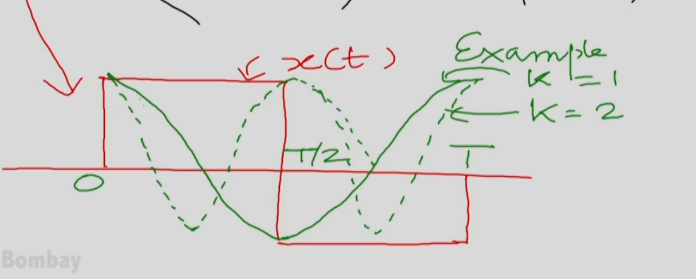
\includegraphics[scale=0.32]{s_216.PNG} %\\Figure 2
\caption{Dot product of the square wave with cosines}	
\end{figure}

\noindent
Calculating  $\langle x(t), \sin (\frac{2\pi}{T}kt)\rangle \cdot \frac{2}{T}\sin (\frac{2\pi}{T}kt)$, we have as shown in Fig.\ref{fig:square-dot-sine},

\begin{figure}[ht]\label{fig:square-dot-sine}
\centering
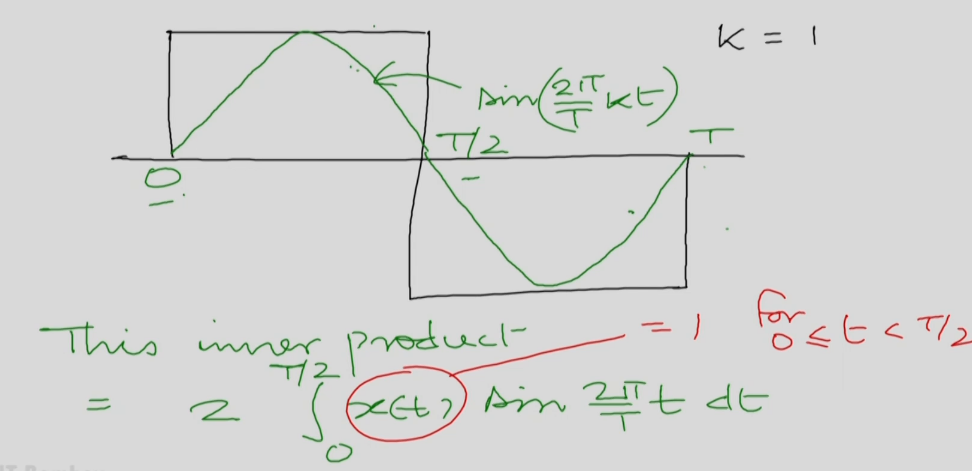
\includegraphics[scale=0.32]{S_216_3.PNG} %\\Figure 3
\caption{Dot product of the square wave with sines}	
\end{figure}
%%%
\begin{equation*} \langle x(t), \sin (\frac{2\pi}{T}kt)\rangle = \int_{0}^{T} \! x(t)\sin (\frac{2\pi}{T}kt) \ \dm t\end{equation*}
\begin{equation*} \langle x(t), \sin (\frac{2\pi}{T}kt)\rangle = \int_{0}^{\frac{T}{2}} \! \sin (\frac{2\pi}{T}kt) \ \dm t + \int_{\frac{T}{2}}^{T} \! {-\sin (\frac{2\pi}{T}kt)} \ \dm t \end{equation*}
\noindent
Also, we know that 
 \begin{equation*}\int_{0}^{\frac{T}{2}} \! \sin (\frac{2\pi}{T}kt) \ \dm t = -\int_{\frac{T}{2}}^{T} \! \sin (\frac{2\pi}{T}kt) \ \dm t \end{equation*}
\noindent
Using this, we have
\begin{equation*} \langle x(t), \sin (\frac{2\pi}{T}kt)\rangle = 2\int_{0}^{\frac{T}{2}} \! \sin (\frac{2\pi}{T}kt) \ \dm t = \left[-2\frac{\cos (\frac{2\pi}{T}kt)}{\frac{2\pi}{T}k}\right]_0^\frac{T}{2}\end{equation*}
%%%
For $k = 2n$, the above integral goes to zero as $\cos ({2\pi}n) = 1$ for all $n \in \mathbb{Z}$.
For $k = 2n-1$, the above integral has the value of $4T/\pi k$ because $\cos(2{\pi}(2n-1)) = -1$ for all $n \in \mathbb{Z}$. Thus,

\begin{equation*} \langle x(t), \sin (\frac{2\pi}{T}kt)\rangle = \frac{4T}{{\pi}k} \textrm{ (for odd }k) \end{equation*}
\noindent
Hence, we have, after multiplying by $2/T$,
\begin{equation*} x(t) = \sum_{n=1}^{\infty}\ \frac{4}{{\pi}(2k-1)} \sin (\frac{2\pi}{T}(2k-1)t)\end{equation*} 

\subsection{Examples of Decomposition}
\subsubsection{Exercise 1} 
\noindent
Work out the decomposition for an asymmetric square wave, of period $T$ as shown in the figure below.
\begin{figure}[ht]
\centering
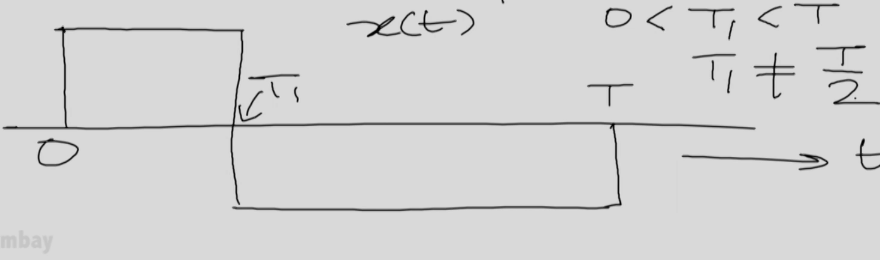
\includegraphics[scale=0.32]{S_217_1.PNG}
\end{figure}
 				\begin{equation*} x(t) = 1 \enspace \enspace      0<t<T_1 \end{equation*}
       			\begin{equation*} x(t) = -1  \enspace\enspace 	T_1 < t< T \end{equation*} \begin{equation*}0<T_1<T, \enspace T1\neq T/2, x(t+T) = x(t)\enspace  \forall t\in R.  \end{equation*}

                
\subsubsection{Exercise 2}
\noindent
In the answer of exercise 1 put $T_1 =T/2$, and verify the answer with that of decomposition of symmetric square wave.

\subsubsection{Exercise 3}
\noindent
Work out the decomposition for symmetric triangular wave, periodic with period $T$.

\noindent
\textit{Hint}: Use and observe the symmetry graphically.
\begin{figure}[ht]
\centering
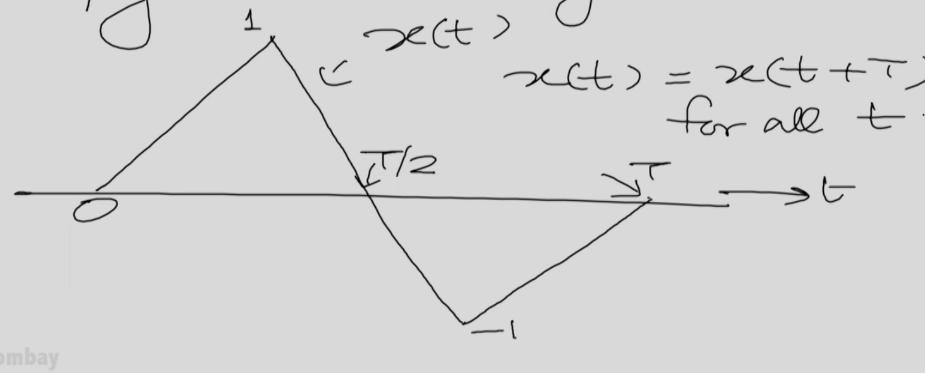
\includegraphics[scale=0.32]{S_217_2.PNG}
\end{figure}


\subsubsection{Exercise 4}
\noindent
Evaluate the decomposition for an asymmetric triangular wave as shown in the figure. Cross check the answer with that of exercise 3, by putting  $T_1 = T/2$ in the final answer.
\begin{figure}[ht]
\centering
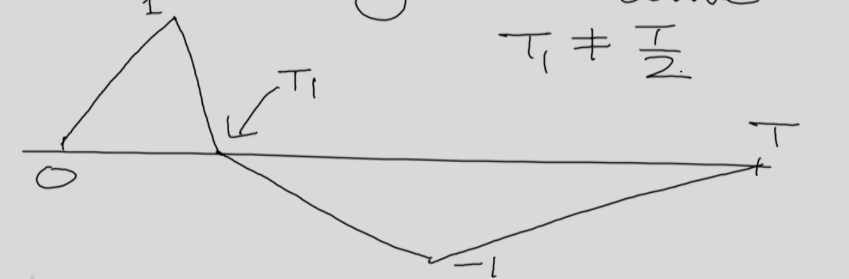
\includegraphics[scale=0.32]{S_217_3.PNG}
\end{figure}


\subsubsection{Exercise 5}
\noindent
A variant of symmetric triangular wave is shown below. Find its decomposition and compare with answer of exercise 3.
\begin{figure}[ht]
\centering
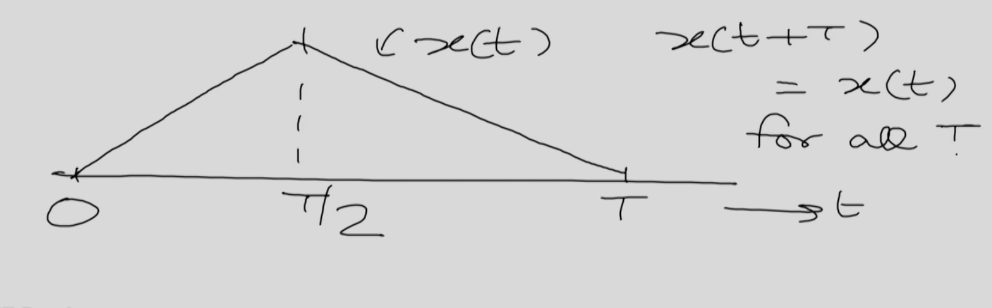
\includegraphics[scale=0.32]{S_217_4.PNG}
\end{figure}

\pagebreak

\subsubsection{Exercise 6}
\noindent
A variant of an asymmetric triangular wave is shown below. Evaluate the decomposition of  this wave. Substitute $T_1 = T/2$, in the answer and compare with the result of exercise 5. Explain the differences in the result, if any.
\begin{figure}[ht]
\centering
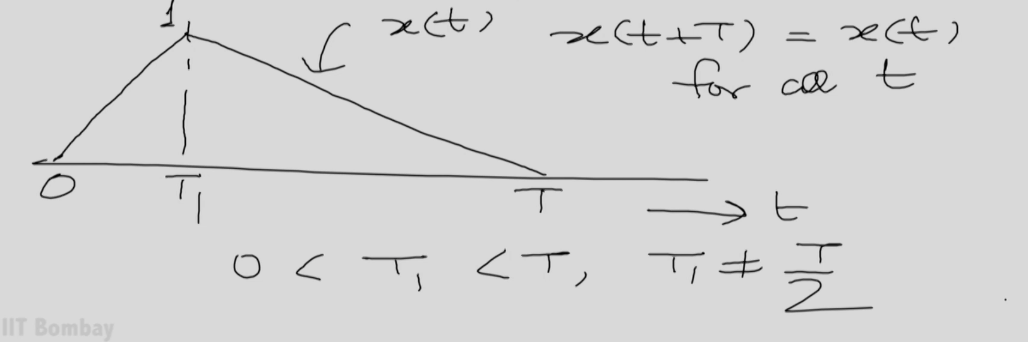
\includegraphics[scale=0.32]{S_217_5.PNG}
\end{figure}








                



                     

\section{Module 2: Lecture 5\\Fourier Series Decomposition and its Applications}

\subsection{Introduction}
We have been decomposing periodic waveform into their periodic sinusoidal components. In this lecture we look at a variation of the same decomposition using complex exponential functions. One way of doing this is to convert each sinusoidal component of sinusoidal decomposition into corresponding exponential functions. However, in some cases, we prefer to a priori decompose the waveform in complex exponential components.
\newline
We shall also see how to go from the complex exponential components to sinusoidal components. We will then look at the applications of both sinusoidal and complex exponential decompositions; in particular, we will be analyzing its utility in determining the output from a linear shift invariant system on applying a periodic input.
We will also see some conditions under which we cannot obtain a Fourier series decomposition for a periodic waveform.

\subsection{Complex Exponential Fourier Series Decomposition}
Suppose we are given a periodic signal $x(t)$ with period $T$. We wish to write $x(t)$ in terms of sum of complex exponential functions:
$$ x(t) = \sum_{k=-\infty}^{\infty}{C_{k} \ e^{j2\pi kt/T}} $$
where $C_k$ belongs to the set of complex numbers.
Basically, we are trying to write $x(t)$ as a linear combination complex exponential functions rotating at angular frequencies $2\pi k/T$ for all integer $k$. Notice that complex exponentials with angular frequencies as positive integral multiples of $2\pi kt/T$ represent anticlockwise rotating phasors while the complex exponentials with negative angular frequencies represent clockwise rotating phasors.
\newline
\subsubsection{Orthogonality of Fourier Series Components}
We now establish orthogonality between the complex exponential components.
We take 2 integers $k$ and $l$ and evaluate the inner product
\begin{equation}
\int_{-T/2}^{T/2}{\frac{1}{T}e^{(j2\pi kt/T)}e^{(j2\pi (-l)t/T)}}dt = \int_{-T/2}^{T/2}{\frac{1}{T}e^{(j2\pi (k-l)t/T)}}dt
\end{equation}
We have 2 cases now:
\begin{itemize}
\item {\textbf{Case 1}} $k=l$ The integral in (1) becomes $\int_{-T/2}^{T/2}\frac{1}{T}dt = 1$
\item {\textbf{Case 2}} $k \neq l$ The integral in (1) becomes $$\int_{-T/2}^{T/2}{\frac{1}{T}e^{(j2\pi (k-l)t/T)}}dt = \frac{1}{T}\frac{e^{(j2\pi (k-l)t/T)}}{(j2\pi (k-l)/T)}\Bigg|_{-T/2}^{T/2} = 0$$
\end{itemize}
\subsubsection{Obtaining Complex exponential Decomposition from Sinusoidal Decomposition}
Suppose we are given the sinusoidal components of the decomposition of a real waveform $$x(t) = \sum_{0}^{\infty}A_{k}\cos(2\pi kt/T + \phi_{k})$$
Note that in the above sum, for $k = 0$, we will have the component as $A_{0}\cos(\phi_{0})$, we can merge constant $\cos(\phi_{0})$ into $A_{0}$ and we will simply have constant $A_{0}$ for $k = 0$.
Now for a non-zero integer $k$ using $\cos(\theta) = \frac{1}{2}(e^{j\theta} + (e^{j\theta})^{*})$, (Note: $C^{*}$ denotes complex conjugate of $C$), we have $$A_{k}\cos(2\pi kt/T + \phi_{k}) = \frac{1}{2}\Bigg(A_{k}e^{j\phi_{k}}e^{j2\pi kt/T} + (A_{k}e^{j\phi_{k}})^{*} (e^{-j2\pi kt/T})\Bigg)$$
since $A_k$ are real.
$$\implies C_{k} = \frac{1}{2}A_{k}e^{j\phi_{k}}$$
$$\implies C_{-k} = \frac{1}{2}(A_{k}e^{j\phi_{k}})^{*}$$
And we also have trivially $C_{0} = A_{0}$
Notice that for real waveform, we have $C_{k} = (C_{-k})^{*}$


\subsubsection{Converting Complex Exponential to Sinusoidal Decomposition}
Suppose we are given a real $$ x(t) = \sum_{k=1}^{\infty}{C_{k}e^{(j2\pi kt/T)}} + \sum_{k=-\infty}^{-1}{C_{k}e^{(j2\pi kt/T)}} + C_{0}$$
Now, note that for an integer $k \neq 0$, $$\int_{-T/2}^{T/2}e^{(j2\pi kt/T)}dt = \frac{1}{T}\frac{e^{(j2\pi kt/T)}}{(j2\pi k/T)}\Bigg|_{-T/2}^{T/2} = 0$$
whereas, for k = 0, $$\int_{-T/2}^{T/2}1dt = T$$
So, basically we can obtain $C_{0}$ by integrating $x(t)$ over time $T$. In the Fourier Decomposition only $C_{0}$ will give a non zero integral which is equal to $C_{0}\cdot T$
Hence, $$C_{0} = \frac{1}{T}\int_{-T/2}^{T/2}x(t)dt$$
Now, since for real $x(t)$ we have $C_{k} = (C_{-k})^{*}$, we get
$$C_{k}e^{j2\pi kt/T} = (C_{-k}e^{-j2\pi kt/T})^{*}$$ So we have $$C_{k}e^{j2\pi kt/T} + C_{-k}e^{-j2\pi kt/T} = 2 Re (C_{k}e^{j2\pi kt/T})$$
Using the polar form of $C_{k}$ which is $|{C_{k}}|e^\phi_{k}$, we get
$$ 2 Re (C_{k}e^{j2\pi kt/T}) =  2|{C_{k}}|Re(e^{j2\pi kt/T + \phi_{k}} = 2|{C_{k}}|\cos(j2\pi kt/T + \phi_{k})$$
Finally, we have the sinusoidal decomposition
$$x(t) = C_{0} + \sum_{k=1}^{\infty}2|{C_{k}}|\cos(j2\pi kt/T + \phi_{k})$$

\subsection{Periodic Input to a Simple RC Circuit}

Suppose, we apply a real periodic voltage waveform $x(t)$ as input to a series RC-circuit with time period $T$. Recall that an RC circuit is a linear shift invariant system. Suppose we can write complex exponential decomposition of $x(t)$ as $$\sum_{k=-\infty}^{\infty}{C_{k}e^{(j2\pi kt/T)}}$$ The advantage of doing this is that we can use the fact that a complex exponential input to a linear shift invariant system simply gives the same complex exponential multiplied by a constant as its ouput. By phasor analysis of the circuit, we have the transfer function $$ \frac{j(2\pi k/T) CR}{1 + j(2\pi k/T) CR}$$
So, the output waveform will be simply $$y(t) = \sum_{k=-\infty}^{\infty} \frac{j(2\pi k/T) CR}{1 + j(2\pi k/T) CR} {C_{k}e^{(j2\pi kt/T)}}$$


This illustrates the power of having complex exponential decomposition of a waveform since we can obtain the output waveform quite simply if it is passed through a linear shift invariant system. Now, one catch in the above discussion is that we assumed that the decomposition of $x(t)$ in to a Fourier series is possible. It turns out it's \emph{not} always the case that we can write a Fourier series decomposition for a periodic waveform! Although, for most of the practical waveforms, we can write it. We will look at the conditions under which we can write the Fourier series decomposition for a periodic waveform. There are some waveforms for which we cannot find the Fourier decomposition. One such example is $x(t) = \sin{(1/frac(t))}$ where $frac(t)$ denotes fractional part of $t$. So, $x(t)$ is periodic with period 1 but still its Fourier series decomposition fails to exist. There are certain conditions under which Fourier analysis can be done, they are called the ‘Dirichlet’ Conditions. We shall not discuss them here.


\subsection{Periodic Inputs to a General Linear Shift Invariant System}

In this section we use Fourier series decomposition to determine output from a linear shift invariant system on applying a periodic input waveform. Of course for our analysis, will assume that Fourier series decomposition of the input waveform exists.
\newline
Let $\mathbb{S}$ denote a linear shift invariant system, let $h(t)$ be its impulse response. We apply a periodic input waveform $x(t)$. Now, using linearity of the system, output of the system is simply the sum of output obtained for each component of Fourier series decomposition of $x(t)$.
\newline
Let us derive the output for the $k^{\textnormal{th}}$ component of $x(t)$. The output for $k^{\textnormal{th}}$ will be the convolution of $h(t)$ and the input itself 
	$$\int_{-\infty}^{\infty}{h(\tau) \cdot C_{k}e^{j2\pi k(t- \tau)/T}}d \tau$$ Since, the above integral runs over $\tau$ and not $t$, the above expression reduces to 
    $$C_{k}e^{j2\pi kt/T}\int_{-\infty}^{\infty}{h(\tau) \cdot e^{-j2\pi k\tau/T}} d \tau$$
The integral reduces to a constant depending on k. So, what we obtain is quite interesting as it is simply the input itself multiplied by a constant!
Let us denote the constant by $\mathcal{H}(k)$. So, the output which is the sum of the outputs obtained for each component is
$$\sum_{k=-\infty}^{\infty}\mathcal{H}(k)C_{k}e^{j2\pi kt/T}$$

\subsection {Conclusion} In this lecture we discussed about Fourier series decomposition, its properties and its application in analysing linear shift invariant systems. In the coming lectures, we will discuss the significance of the quantity $\mathcal{H}(k)$ we derived in previous section and begin with what is known as Fourier Transform.







\chapter{The Fourier Transform}
\section{Module 2: Lecture 6\\The Fourier Transform}

\subsection{Introduction}
We are now in a position where we can deal with more general signals from the point of view of decomposition into sinusoidal frequency components and analysis as to what happens when you pass them through a linear shift invariant system. To do that, let's recapitulate some of the important conclusions that we had drawn in the previous chapter which will now help us in generalization.
%%%
%%%
\subsection{Recapitulation}
Let $\mathbb{S}$ be a linear shift invariant system with impulse response $h(t)$, and to it, we give a periodic signal input. Let’s assume that the Dirichlet conditions are obeyed. So we could decompose this into its Fourier series.
\begin{equation*}
x(t)= \sum\limits_{k=-\infty}^{k=+\infty}c(k)e^{j\Omega kt}
\end{equation*}
Where $\Omega=2\pi /T$ is the angular frequency and $c(k)$ are the Fourier coefficients. Now, the output can also be written as a Fourier series.
\begin{equation*}
y(t)= \sum\limits_{k=-\infty}^{k=+\infty}c(k)H(k\Omega)e^{j\Omega kt}
\end{equation*}
where
\begin{equation*}
H(\Omega)= \int_{-\infty}^{+\infty} \! h(t)e^{-j\Omega t} \ \dm t
\end{equation*}
%%%
%%%
\subsection{Interpretation of $H(\Omega)$ as a Dot Product}
We can interpret $H(\Omega)$ as a dot product or inner product. It’s an inner product between the impulse response $h(t)$ and the rotating phasor $e^{j\Omega t}$. An inner product with a unit vector calculates the projection or a component of the vector along the unit vector. So it's as if we are trying to find the component of the impulse response along a rotating phasor, rotating with an angular velocity $\Omega$. And, at the specific values of $\Omega$ given by each of the Fourier series components, we evaluate this dot product and use it to modify the Fourier series coefficient.
We can see from the equation of output $y(t)$ that output Fourier series coefficients are $c(k)H(\Omega k)$. Recall that in the input, the Fourier series coefficients were calculated by taking an inner product taking only one period of the input for the integral.
We took only one period of the input, and found the inner product with the corresponding harmonic or the complex exponential rotating with that particular multiple of the fundamental frequency. This is how we calculate the Fourier series coefficients.\\
Now, we can see that the Fourier coefficients of the output are the \emph{component by component multiplication of the Fourier coefficients of the input and impulse response}.
\[
Y(k\Omega)= c(k)H(k\Omega)
\]
Now, there are two questions to answer here. Here we have assumed that the input was periodic. What if it is not? Can we generalize this to a non-periodic function is a question that we need to answer. Secondly, can we think of this quantity $H(\Omega)$ as a new transform or a new way of dealing with the impulse response in its own right?\\
Now, a transform will make sense or will be adequate only if it is invertible. That is to say, we should be able to get back $h(t)$ from $H(\Omega)$. There should be no loss of information. It turns out that this is indeed the case. We can call $H(\Omega)$, for any $\Omega \in \mathbb{R}$, as the \emph{Fourier transform} of the impulse response $h(t)$.\\
Now let's try to address the question as to how can we \emph{go back} to $h(t)$ from $H(\Omega)$.
%%%
%%%
\subsection{Inverse for the Fourier Transform}
The answer to the question again lies in vector intuition. As we have seen, $H(\Omega)$ is the component of $h(t)$ along the phasor $e^{j\Omega t}$ for all such $\Omega \in \mathbb{R}$. In vector algebra, we get back a vector from its components by multiplying the components with their corresponding unit vectors and summing them. So, if $\hat{u}_1$ and $\hat{u}_2$ are two orthogonal unit vectors in two dimensions, $\overrightarrow{v}$ is a 2-D vector, and
\[
\langle \overrightarrow{v},\hat{u}_1 \rangle = v_1, \langle \overrightarrow{v},\hat{u}_2 \rangle = v_2
\]
Then, we construct $\overrightarrow{v}$ by multiplying the components with the corresponding unit vector and summing them. Hence
\[
\overrightarrow{v} = v_1\hat{u}_1 + v_2\hat{u}_2
\]
Now using the same principle here, $H(\Omega)$ are the components of the ``vector'' $h(t)$ along the unit vectors $e^{j\Omega t}$. Hence, to obtain the vector $h(t)$ back, we should multiply the component by the unit vector and sum up, or in this case, integrate over all $\Omega$.\\
But there are two subtleties involved here. Firstly, we don't know whether in this vector space of integrable functions, the vector $e^{j\Omega t}$ is a unit vector or not. That is, whether its magnitude is one or not. In case it is not one, we have to multiply it by a suitable constant to make it a unit vector. Secondly, we don't know whether $e^{j\Omega_1 t}$ and $e^{j\Omega_2 t}$ are orthogonal or not, for $\Omega_1 \neq \Omega_2$.\\
In the following subsection, we proceed to evaluate the inverse of $H(\Omega)$ assuming two things; one is that the vectors $e^{j\Omega t}$ are orthogonal, and that the multiplying factor $\kappa_0$ (for making it a unit vector) is independent of $\Omega$.
%%%
%%%
\subsubsection{Finding the Inverse of the Fourier Transform}
Form the previous discussion, the quantity we propose to be the inverse of $H(\Omega)$ is given by
\[
I = \int_{-\infty}^{\infty} \! H(\Omega)\ \kappa_0 e^{j\Omega t} \ \dm \Omega
\]
Now, we know that
\[
H(\Omega)= \int_{-\infty}^{\infty} \! h(t_1)e^{-j\Omega t_1} \ \dm t_1
\]
Putting this in $I$, we get,
\[
I = \int_{-\infty}^{\infty} \! \int_{-\infty}^{\infty} \! h(t_1)e^{-j\Omega t_1}\ \dm t_1 \ \kappa_0 e^{j\Omega t} \ \dm \Omega
\]
\[
= \int_{-\infty}^{\infty} \! h(t_1) \left\lbrace \int_{-\infty}^{\infty} \! \kappa_0 e^{-j\Omega t_1} \  e^{j\Omega t} \ \dm \Omega \right\rbrace \dm t_1
\]
Let's evaluate the quantity in the braces. We can write it as
\[
\lim_{\Omega_1 \to \infty} \int_{-\Omega_1}^{+\Omega_1} \! \kappa_0 e^{j\Omega (t-t_1)} \ \mathrm{d}\Omega
\]

\[
= \lim_{\Omega_1 \to \infty} \kappa_0 \frac{e^{j\Omega_1 (t-t_1)}-e^{-j\Omega (t-t_1)}}{j(t-t_1)}
\]

\[
= \lim_{\Omega_1 \to \infty}\frac{2\kappa_0 j\sin(\Omega_1 (t-t_1))}{j(t-t_1)}
\]

\[
= \lim_{\Omega_1 \to \infty}\frac{2\kappa_0\Omega_1\sin(\Omega_1 (t-t_1))}{\Omega_1(t-t_1)}
\]

Now, this can be written as 
\[
\lim_{\Omega_1 \to \infty} 2\kappa_0\Omega_1 \frac{\sin(x)}{x}
\]
where $x=\Omega_1(t-t_1)$. Now, $\sin(x)/x$ is not defined at $x=0$ as it has a zero divided by zero form. So we evaluate the limit as $x\to 0$.
\[
\lim_{x \to 0}\frac{\sin(x)}{x} = \lim_{x \to 0}\frac{\cos(x)}{1} = 1
\]
where the first equality is due to L'H\^opital's rule. This function will be oscillatory due to $\sin(x)$, but will decay as $x$ increases, due to the $x$ in the denominator. Also, the function will be zero when $x=n\pi$ or $\Omega_1(t-t_1)=n\pi$. Now, let's deal with this function as a function of $(t-t_1)$ rather than $x$. Let us try to plot the function
\[
f(t-t_1) = \frac{2\kappa_0\Omega_1\sin(\Omega_1 (t-t_1))}{\Omega_1(t-t_1)}
\]
The value of $\sin(x)/x$ is $1$ as $x \to 0$ as we saw earlier. Hence $f(0)=2\kappa_0\Omega_1$. Also the first null of the function will occur at $\Omega_1(t-t_1)=\pi$ or $(t-t_1)=\pi/\Omega_1$. Also the function is even with respect to $(t-t_1)$.
\begin{figure}[ht]
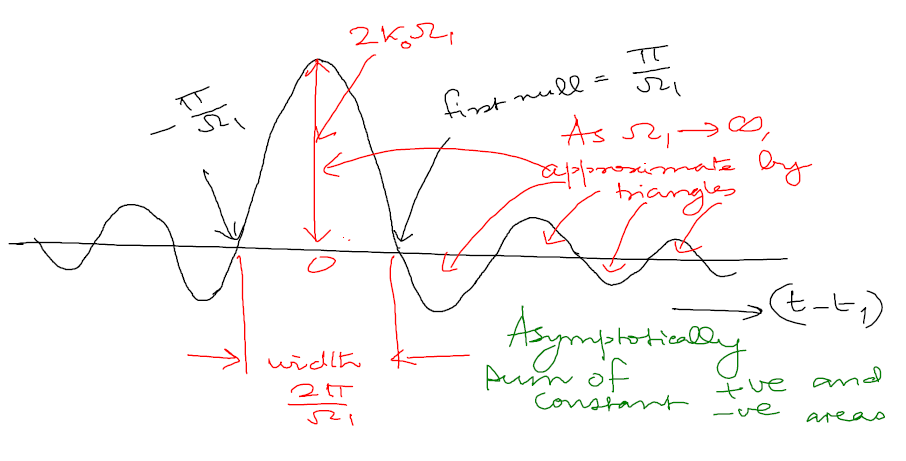
\includegraphics[scale=0.6]{fig.png}
\label{fig:sinc}
\caption{Sinc function}
\end{figure}
Hence, we will get a plot roughly as shown in Fig.\ref{fig:sinc}.
Now, we have to look at what happens when $\Omega_1 \to \infty$. We can see that the height of the main lobe at $x=0$ goes to infinity, but the width of the lobe, which is $2\pi/\Omega_1$ goes to zero, as $\Omega_1 \to \infty$. It can also be shown that the area of the other smaller lobes add up to zero, due to their alternating nature. Hence, we have a \emph{pulse} whose height is tending to infinity and the width to zero. In that case, we can assume the central lobe to be a triangle. Hence its area will be
\[
A = \frac{1}{2}\frac{2\pi}{\Omega_1}2\kappa_0\Omega_1 = 2\pi\kappa_0
\]
Hence, we can see that this area is a constant independent of $\Omega_1$. So we have a pulse having infinite magnitude and zero width, with a constant area encapsulated by it, and as you will remember from Part 1, this is nothing but the \emph{impulse function} $2\pi\kappa_0\delta(t-t_1)$.\\
Now, going back to our integral $I$,
\[
I = \int_{-\infty}^{\infty} \! h(t_1) \left\lbrace \int_{-\infty}^{+\infty} \! \kappa_0 e^{-j\Omega t_1} \  e^{j\Omega t} \ \mathrm{d}\Omega \right\rbrace \mathrm{d}t_1
\]
And we have evaluated the quantity in the braces to be $2\pi\kappa_0\delta(t-t_1)$. Hence,
\[
I = \int_{-\infty}^{\infty} \! h(t_1)\left\lbrace 2\pi\kappa_0\delta(t-t_1) \right\rbrace \mathrm{d}t_1 = 2\pi\kappa_0 \int_{-\infty}^{\infty} \! h(t_1) \delta(t-t_1)\ \mathrm{d}t_1
\]
Hence, by the sifting property of the delta function, we have,
\[
I = 2\pi\kappa_0 h(t)
\]
Hence, we can now set the value of $\kappa_0$ such that $I = h(t)$ as required. Hence $\kappa_0 = 1/2\pi$.\\
Hence, we finally have our expression for the \emph{Inverse Fourier transform} of $H(\Omega)$.
\[
h(t) = \frac{1}{2\pi}\int_{-\infty}^{\infty} \! H(\Omega)\  e^{j\Omega t} \ \mathrm{d}\Omega
\]
%%%
%%%
\subsection{Orthogonality of the Complex Exponentials}
A valid question to ask here is where did the orthogonality of the complex exponentials come in the picture. The answer lies in the integral in the braces which we evaluated.
\[
\int_{-\infty}^{+\infty} \! \kappa_0 e^{-j\Omega t_1} \  e^{j\Omega t} \ \mathrm{d}\Omega = 2\pi\kappa_0 \delta(t-t_1)
\]
or,
\[
\int_{-\infty}^{+\infty} \! e^{j\Omega t} \ \overline{e^{j\Omega t_1}} \ \mathrm{d}\Omega = 2\pi \delta(t-t_1)
\]
where the bar indicates complex conjugate. Now, this can be also written by renaming the variables, treating $t$ as the independent variable, as
\[
\int_{-\infty}^{+\infty} \! e^{j\Omega_1 t} \ \overline{e^{j\Omega_2 t}} \ \mathrm{d}t = 2\pi \delta(\Omega_1-\Omega_2)
\]
Now, we can immediately see that this is like an inner product between phasors rotating with different frequencies $\Omega_1$ and $\Omega_2$, and what this statement says is that it is non zero only for $\Omega_1=\Omega_2$. Hence, we do have some sense of orthogonality here. But since the value is infinite when the frequencies are equal, we have to call this a generalized orthogonality relation.
%%%
%%%
\subsection {Implications} 
Let's try to find what the Fourier transform expression implies. We have a non-periodic function $h(t)$ and we have decomposed it in its Fourier coefficients, not for discrete, but continuous set of frequency values, from minus to plus infinity. This can be thought of in the following way: We think of a non-periodic function as a periodic function with period tending to infinity. This is a valid statement, because as a periodic with period $T$ repeats itself after an interval $T$, we can say that a non-periodic function repeats itself after $T \to \infty$. Now, as the time period increases, the spacing between two adjacent frequencies decreases. And
\[
f = \lim_{T\to\infty}\frac{2\pi}{T} = 0.
\]
Hence, for a non-periodic function, the spacing between the adjacent frequencies tends to zero, which amounts to the Fourier spectrum going to continuous from discrete. This is exactly what has happened. The Fourier transform $H(\Omega)$ is a continuous function, and in general has a non-zero value for all $\Omega \in \mathbb{R}$.






\section{Module 2: Lecture 7\\Fourier Transforms properties and Fourier series example}

\subsection{Introduction}
	In this section, we will take a few examples of the calculation of the Fourier transform and then build upon the general properties of a Fourier transform like linearity, time shift, modulation and convolution. \\
	Let us start with calculating the Fourier transform of a rectangular pulse.
\subsection{Fourier transform of a Rectangular Pulse}
	Let the pulse be symmetric, with height equal to $A$, going from $-T/2$ to $T/2$ on the time axis. We call this function $h(t)$ as shown in Fig.\ref{fig:rectangular_pulse}.
	%%%
	\begin{figure}[htp]
		\centering
		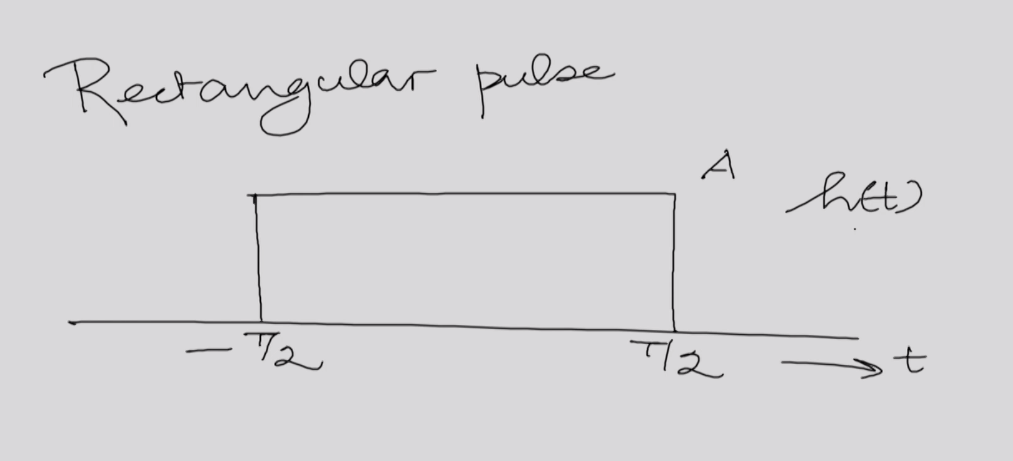
\includegraphics[width=12cm]{rectangularpulse.png}
		\caption{Symmetric Rectangular Pulse}
		\label{fig:rectangular_pulse}
	\end{figure}
	%%%
	Let us denote the Fourier transform by $ H(\Omega)$. Then
	\begin{equation}
		H(\Omega)=\int_{-\infty}^{\infty} \! {h(t) e^{-j\Omega t}} \ \dm t
	\end{equation}
	As $h(t)$ is zero except in the time interval $-T/2$ to $T/2$, we can write the above equation as
	\begin{equation}
		H(\Omega)=\int_{-T/2}^{T/2} \! {A e^{-j\Omega t}} \ \dm t =
		\frac{A e^{-j\Omega t}}{-j \Omega} \Bigg|_{-T/2}^{T/2}=
		\frac{A(e^{-j\Omega T/2}-e^{j\Omega T/2})}{-j\Omega}
		=\frac{AT (2j\sin({\Omega T/2}))}{j\Omega T}
	\end{equation}

	\begin{equation}
		H(\Omega)=\frac{AT\sin({\Omega T/2})}{\Omega T/2}
	\end{equation}
	And we can rewrite it as

	\begin{equation}
		H(f)=\frac{AT \sin({2\pi f T/2})}{2\pi f T/2}
	\end{equation}
	Where $f = \cfrac{\Omega}{2\pi}$ corresponds to the ${cycles}/{second}$ frequency, and $\Omega$ is of course the angular frequency.
	Now this expression also can be written as
	\begin{equation}
		H(\gamma)=\frac{AT \sin({\pi \gamma})}{\pi \gamma}
	\end{equation}
	Where $\gamma = f*T $.\\
	The function $\cfrac{\sin{\pi \gamma}}{\pi \gamma}$ is a very special function called a \emph{Sinc Function}. The sinc function in the form presented is often used in the context of signals and systems.

	\subsubsection{Sketch of the Sinc function}

		Here are the some properties of the Sinc function.
		\begin{itemize}
			\item It is an even function.
			\item It has nulls at every integer; so at 1, at 2, at 3 and so on, it will have value equal to zero.
			\item It tends to 1 as $\gamma$ tends to 0
			\item It is a damped sinusoid, i.e. the magnitude of oscillation decreases as $\gamma$ increases.
		\end{itemize}
		Using the above points we can sketch the Sinc function. So the sketch somewhat looks like Fig\ref{fig:sinc}.
		\begin{figure}[htp]
			\centering
			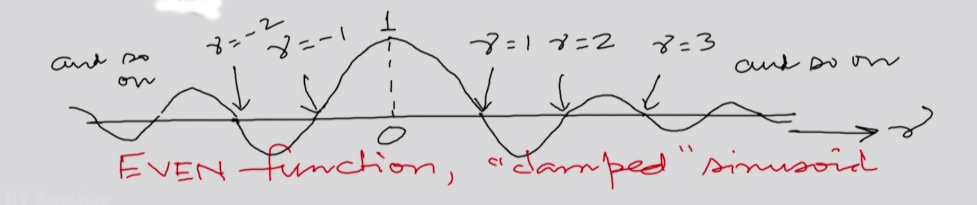
\includegraphics[width=12cm]{sinc.png}
			\caption{Sinc Function}
			\label{fig:sinc}
		\end{figure}

	\subsubsection{Important points regarding the Fourier transform of rectangular pulse}
		The pulse is limited in terms of its occupancy of the time axis. It goes only from  $-T/2$ to $+T/2$. On the other hand, the Fourier transform, in principle, lasts all over the frequency axis.
		What this means is that if we want to make a function vanish all over the time axis outside a certain finite interval, we have to bring together frequencies of all magnitudes and signs except for a few nulls.
		All these frequencies need to come together, in appropriate amplitudes, to form this rectangular pulse. Also note that the Fourier transform for this case is purely real. \\
		 When the pulse width is halved, the nulls of the Fourier transform are doubly spaced and the central amplitude is halved. This can be checked mathematically. We can see that Fig\ref{fig:pulse_FT_half}.
		\begin{figure}[htp]
			\centering
			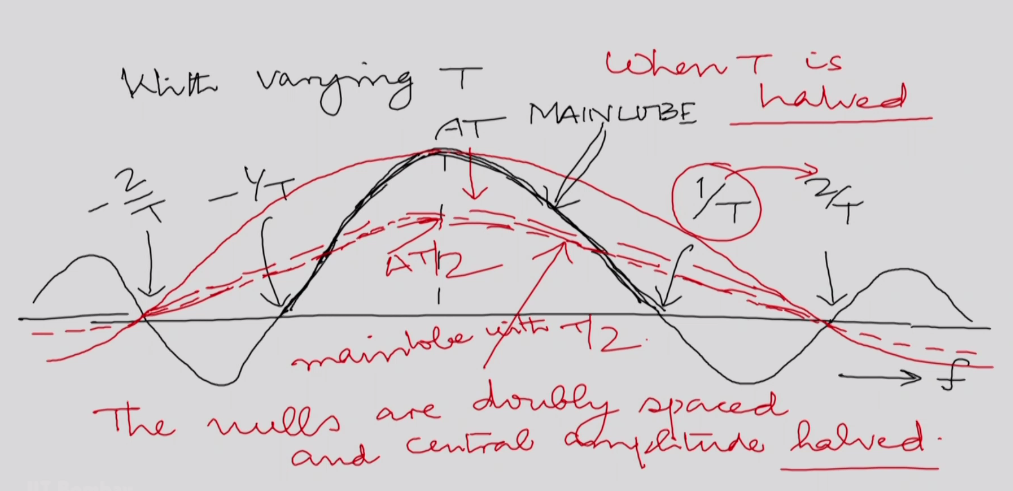
\includegraphics[width=12cm]{pulse_FT_half.png}
			\caption{Fourier Transform of Rectangular Pulse at width T and T/2 }
			\label{fig:pulse_FT_half}
		\end{figure}

\subsection{Properties of Fourier Transform}
	Let us see what happens to the Fourier transform when we change the original signal in some particular way.
	% When we change the signal in some way or when we bring signals together, what happens to the corresponding Fourier transform is what we will investigate in this section.
	\subsubsection{Linearity}
		Let $h_1(t)$ have the Fourier transform $H_1(\Omega)$ and let $h_2(t)$ have the Fourier transform $H_2(\Omega)$. Then, linearity says

		%\begin{equation}
		%$$\alpha h_1(t) + \beta h_2(t) \longrightarrow \alpha H_1(\Omega)+ \beta H_2(\Omega)$$
		%\end{equation}


		\[\alpha h_1(t) + \beta h_2(t) \xrightarrow{\mathcal{F}} \alpha H_1(\Omega)+ \beta H_2(\Omega)\]
		for all $\alpha$, $\beta$ $\in \mathbb{C}$ and all $h_1(t)$ and $h_2(t)$. Here, ${\mathcal{F}}$ means ``has the Fourier transform given by".

	\subsubsection{Proof of linearity}
		\begin{equation}
			 \alpha \{ H_1(\Omega) \} = \alpha \{ \int_{-\infty}^{\infty} \! h_1(t)e^{-j\Omega t} \ \dm t \}
			\label{eqn:one}
		\end{equation}

		\begin{equation}
			 \beta \{ H_2(\Omega) \} = \beta \{ \int_{-\infty}^{\infty} \! h_2(t)e^{-j\Omega t} \ \dm t \}
			\label{eqn:two}
		\end{equation}
		Add Eqn.\ref{eqn:one} and \ref{eqn:two}. We can write it as
		\begin{equation}
			\{ \alpha H_1(\Omega) + \beta H_2(\Omega) \} = \{ \int_{-\infty}^{\infty} \! (\alpha h_1(t) + \beta h_2(t))e^{-j\Omega t} \ \dm t \}
		\end{equation}

	\subsubsection{The Inverse Fourier transform}
		THe Inverse Fourier transform can be written as
		\begin{equation}
			H_1(\Omega) \xrightarrow{\mathcal{F}^{-1}} \frac{1}{2\pi} \int_{-\infty}^{\infty} \! H_1(t) e^{j\Omega t} \ \dm \Omega
		\end{equation}
		Note that $\Omega$ = $2\pi f$ and $d\Omega$= $2\pi df$. Hence,
		%%%
		\begin{equation}
			H_1(f) \xrightarrow{\mathcal{F^-1}} \int_{-\infty}^{\infty} \! H_1(f) e^{j2\pi ft} \ \dm f
		\end{equation}
		%%%
		Where $\Omega$ =  Radians/sec frequency
		And $f$ = cycles/sec frequency
		%%%
		\begin{itemize}
			\item We can clearly see that when frequency is in radians/sec then, we will have factor of $1/2\pi$ in the inverse Fourier transform and when frequency is in cycles/sec then the factor of $1/2\pi$ will not be there.
			\item In a way dealing with cycles/second frequency has some conveniences; we don't need to remember the factor of $1/2\pi$, or we can say, there is a perfect symmetry between the Fourier transform and the Inverse Fourier transform.
		\end{itemize}

	\subsubsection{Exercise}
		 Prove that linearity holds true for the inverse Fourier transform.

\subsection{Time Shift}
	What happens to the Fourier transform when we shift the signal in time? If
	\begin{equation}
		h(t) \xrightarrow{\mathcal{F}} H(\Omega)
	\end{equation}
	then, for a constant $\tau$,
	\begin{equation}
		h(t-\tau) \xrightarrow{\mathcal{F}} {?}
	\end{equation}
	%%%
	The Fourier transform would be
	\begin{equation}
		H(\Omega) =  \int_{-\infty}^{\infty} \! h(t-\tau) e^{-j\Omega t} \ \dm t
	\end{equation}
	Put $(t-\tau) = \lambda$  $\Rightarrow$  $t = \tau + \lambda$.
	So the Fourier transform is
	\begin{equation}
		H(\Omega) =  \int_{-\infty}^{\infty} \! h(\lambda) e^{-j\Omega (\lambda + \tau)} \ \dm \lambda =
		e^{-j\Omega \tau} \int_{-\infty}^{\infty} \! h(\lambda) e^{-j\Omega \lambda} \ \dm \lambda
	\end{equation}
	So,
	\begin{equation}
		h(t-\tau) \xrightarrow{\mathcal{F}} e^{-j\Omega \tau} H(\Omega)\   or\   e^{-j2\pi f\tau} H(f)
	\end{equation}
	Now it can be clearly seen that
	\begin{itemize}
		\item The magnitude of the Fourier transform is unchanged.
		\item The angle or the phase of the Fourier transform changes.
	\end{itemize}

	\subsubsection{Modulation}
		By modulation, we mean multiplying $h(t)$ by a rotating complex number (rotating with an angular velocity of $\Omega_0$). In this case, the Fourier transform is shifted by $\Omega_0$ forward.

		\begin{equation}
			e^{j\Omega_0 t} h(t) \xrightarrow{\mathcal{F}} {?}
		\end{equation}
		So the Fourier transform would be
		\begin{equation}
			 \int_{-\infty}^{\infty} \! e^{j\Omega_0 t} h(t) e^{-j\Omega t} \ \dm t =
			 \int_{-\infty}^{\infty} \! h(t) e^{-j(\Omega-\Omega_0) t} \ \dm t =
			 H(\Omega-\Omega_0)
		\end{equation}
		
		\begin{itemize}
			\item When we shift a function in time, it causes a modulation in the frequency domain (We remember, it multiplied the Fourier transform by a term $e^{-j\Omega \tau_0}$).

			\item When we modulate the function in time by multiplying by a rotating complex number, the corresponding Fourier transform shifts in frequency.

			\item Basically, shift in time becomes modulation in frequency, and modulation in time becomes a shift in frequency.
		\end{itemize}

	\subsubsection{Convolution Property of Fourier transform}
		The question to answer here is what will be the Fourier transform of $x_1(t)*x_2(t)$, given that the Fourier transforms of $x_1(t)$ and $x_2(t)$ are $X_1(\Omega)$ and $X_2(\Omega)$ respectively. 

		\begin{equation}
			x_1(t)\ast x_2(t) = \int_{-\infty}^{\infty}{x_1(\tau) x_2(t-\tau)}d\tau
		\end{equation}

		\begin{equation}
			x_1(t)\ast x_2(t) \xrightarrow{\mathcal{F}} {?}
		\end{equation}
		\noindent
		Now let's solve it. The Fourier transform can be written as
		\begin{equation}
			\int_{-\infty}^{\infty} \! \{ \int_{-\infty}^{\infty} \! x_1(\tau) x_2(t-\tau) \ \dm \tau \} e^{-j\Omega t} \ \dm t
		\end{equation}
		This is same as
		\begin{equation}
			\int_{-\infty}^{\infty} \! \int_{-\infty}^{\infty} \! x_1(\tau) x_2(t-\tau) e^{-j\Omega t} \ \dm \tau \dm t
		\end{equation}
		To solve the above double integral we will do a change of variables. Put
		\begin{equation}
			\alpha =\tau \ \text{and} \ \beta = (t-\tau)
		\end{equation}

		\begin{equation}
			\left( \begin{array}{c}
			\alpha \\
			\beta \end{array} \right)
			=
			\left( \begin{array}{cc}
			1 & 0 \\
			-1 & 1 \end{array} \right)
			\left( \begin{array}{c}
			\tau \\
			 t \end{array} \right)
		\end{equation}

		\begin{equation}
			\mathrm{d}\tau \mathrm{d}t = |\text{Det(transformation)}| \mathrm{d}\alpha \mathrm{d}\beta
		\end{equation}
		\noindent
		Hence,
		\begin{equation}
			\mathrm{d}\tau \mathrm{d}t = \mathrm{d}\alpha \mathrm{d}\beta
		\end{equation}
		Hence, the element of integration also remains the same because the Jacobian is $1$. Now the modified integral is
		
		\begin{equation}
			\int_{-\infty}^{\infty} \! \int_{-\infty}^{\infty} \! x_1(\alpha) x_2(\beta) \exp{-j\Omega(\alpha+\beta)} \ \dm \alpha \dm \beta
		\end{equation}
		
		\begin{equation}
			=\int_{-\infty}^{\infty} \! x_1(\alpha) \{ \int_{-\infty}^{\infty} \!
			x_2(\beta) e^{-j\Omega(\beta)} \ \dm \beta \} e^{-j\Omega \alpha} \ \dm \alpha
		\end{equation}
		This can be written as
		
		\begin{equation}
			X_2(\Omega) \int_{-\infty}^{\infty} \! x_1(\alpha) e^{-j\Omega \alpha} \ \dm \alpha
		\end{equation}
		So
		\begin{equation}
			x_1(t) \ast x_2(t) \xrightarrow{\mathcal{F}} X_1(\Omega)X_2(\Omega)
		\end{equation}
		\noindent
		Hence a convolution in the natural domain becomes a multiplication in the Fourier domain.

\subsection {Conclusion} In this section, we discussed about the Fourier transform of a rectangular pulse which is the ``Sinc function'', and its properties. We showed some of the properties of Fourier transform and their proofs.
\section{Module 2: Lecture 8\\Convolution Property of the Fourier Transform}

\subsection{Introduction}
	In this section, we will talk about the properties of the Fourier transform and specifically, we see more about the convolution property.
\subsection{Convolution Theorem}
	If two signals $x_1(t)$ and $x_2(t)$ both have Fourier transforms, which are $X_1(\Omega)$ and $X_2(\Omega)$ respectively, and if their convolution also has a Fourier transform, then this Fourier Transform is equal to the product of $X_1(\Omega)$ and $ X_2(\Omega)$.\\
	Mathematically,
	\begin{align}
		x_1(t) \xrightarrow{\mathcal{F}}& X_1(\Omega)\\
		x_2(t)\xrightarrow{\mathcal{F}}& X_2(\Omega)\\
		x_1(t)*x_2(t)\xrightarrow{\mathcal{F}}& X_1(\Omega).X_2(\Omega)
	\end{align}
	So, when we apply it to the context of LSI systems, we get
	\begin{equation}
		Y(\Omega)=X(\Omega)H(\Omega)
	\end{equation}
	where,
	\begin{align}
		x(t) &\xrightarrow{\mathcal{F}} X(\Omega)\\
		y(t) &\xrightarrow{\mathcal{F}} Y(\Omega)\\
		h(t) &\xrightarrow{\mathcal{F}} H(\Omega)
	\end{align}
	\begin{figure}[ht]
		\centering
		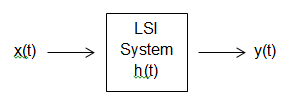
\includegraphics{fig0.png}
		%\caption{\label VVoltage generator (side view)}
	\end{figure}
	We said that there is a point-wise decoupling or memorylessness in the Fourier domain, meaning, the output at angular frequency $\Omega$ depends only on the input at angular frequency $\Omega$ and the impulse response at angular frequency $\Omega$ and none other.\\
	Where does this come from?\\
	$X(\Omega)$ is the component of input at angular frequency $\Omega$. Let us imagine $X(\Omega)e^{j\Omega t}$ as an input to the LSI system, where $X(\Omega)$ is a complex number.\\
	We have,
	\begin{figure}[h!]
		\centering
		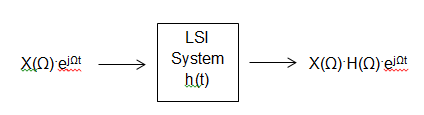
\includegraphics{fig1.png}
		%\caption{\label VVoltage generator (side view)}
	\end{figure}
	\begin{align}
		y(t) &= \int_{-\infty}^{\infty} \! h(\tau) X(\Omega) \ e^{j\Omega (t-\tau)} \ \dm \tau\\
		&= \left( \int_{-\infty}^{\infty} \! h(\tau) \ e^{-j\Omega \tau} \ \dm \tau \right) X(\Omega) \ e^{j\Omega t}\\
		&= X(\Omega) H(\Omega) \ e^{j\Omega t}
	\end{align}
	$H(\Omega)$ is the component of the impulse response along $e^{j\Omega t}$. Hence, $X(\Omega).H(\Omega)$ is the component of $y(t)$ along $e^{j\Omega t}$ and is equal to $Y(\Omega)$.\\
	\begin{equation}
		Y(\Omega)=X(\Omega).H(\Omega)
	\end{equation}
	%%%
	%%% CHECK THE FOLLOWING PART:
	This is analogous to an operator acting upon a force in mechanics. If $\nabla$ is the operator and if $\vec{F}$ the force vector such that
	\begin{equation}
	\vec{F}=F_x \hat{x} + F_y \hat{y} + F_z \hat{z}
	\end{equation}
	Then
	\begin{eqnarray}
	\nabla . \vec{F} &=& \nabla . (F_x \hat{x} + F_y \hat{y} + F_z \hat{z})\\
	\nabla . \vec{F} &=& \partial_x F_x \hat{x} + \partial_y F_y \hat{y} + \partial_z F_z \hat{z}\\
	\end{eqnarray}
	Similarly we resolve the input into its components along the different $\Omega$'s, i.e. $ej\Omega  t$.
	\begin{eqnarray}
	x(t)&=&\sum_i X(\Omega_i).\textrm{exp}(j\Omega_i t)\\
	y(t)&=&\sum _i X(\Omega_i).H(\Omega_i).\textrm{exp}(j\Omega_i t)
	\end{eqnarray}
	In a way, the idea is to decouple the action of the LSI system when we think of the input as comprising of different complex exponentials rotating at different angular frequencies, both positive and negative.
	%%%
	%%%
\subsection{What is a transform?}
	More generally, transform is a change of paradigm. Paradigm means world view. In a system point of view, a signal is a mapping from the independent variable to complex numbers, while a system is a mapping from signals to signals. Whereas a transform is a mapping of the signals and systems altogether to the transformed domain of signals and systems.
\subsection{Convolution or Multiplication}
	Doing multiplication, in general, is easier than convolution. To find the convolution, take Fourier transforms of the two signals, multiply them and then take its inverse Fourier transform.
	\begin{align}
		x_1(t) &\xrightarrow{\mathcal{F}} X_1(\Omega)\\
		x_2(t) &\xrightarrow{\mathcal{F}} X_2(\Omega)\\
		X_1(\Omega).X_2(\Omega) &\xrightarrow{\mathcal{F}^{-1}} x_1(t) \ast x_2(t)
	\end{align}
	It is beneficial only if the Fourier transform operations are easier to perform, otherwise it is not always better to go through the Fourier domain.\\
	For example, take $x_1(t)=x_2(t)$ as a rectangular pulse as shown in Fig\ref{fig:rectangular_pulse}.
	\begin{figure}[h!]\label{fig:rectangular_pulse}
		\centering
		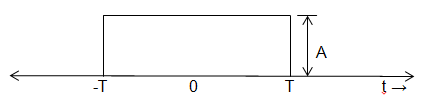
\includegraphics{fig2.png}
	\end{figure}
	Hence,
	\begin{align}
		X_1(\Omega)=X_2(\Omega) &= \int_{-\infty}^{\infty} \! x_1(t) \ e^{-j\Omega t} \ \dm t\\
		&= \int_{-T}^{T} \! A \ e^{-j\Omega t} \ \dm t\\
		&= \left(\frac{A}{-j\Omega} \ e^{-j\Omega t}\right) \Bigg|_{-T}^{T}\\
		&= \frac{2Aj \sin(\Omega t)}{j\Omega} \times \frac{T}{T}\\
		&= 2AT \frac{\sin{\Omega T}}{\Omega T}
	\end{align}
	Whereas the convolution leads to
	\begin{equation}
		x_1(t) \ast x_2(t)=\int_{-\infty}^{\infty} \! x_1(\tau)x_2(t-\tau) \ \dm \tau
	\end{equation}
	Now, $x_1(\tau) x_2(t-\tau)$ is non-zero only when some area of both the pulses coincide and is non- zero for that range only.
	This happens only for $t \in [-2T,2T]$
	\begin{figure}[h!]
	\centering
	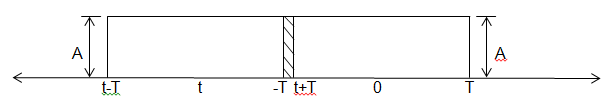
\includegraphics[scale=0.9]{fig3.png}
	\end{figure}
	Therefore, for $t \in [-2T,0]$
	\begin{align}
		x_1(t) \ast x_2(t) &= \int_{-\infty}^{\infty} \! x_1(\tau)x_2(t-\tau) \ \dm \tau\\
		&= \int_{-T}^{t+T} \! A^2 \ \dm \tau \\
		&= A^2 (t+2T)
	\end{align}
	and for $t \in [0,2T]$
	\begin{align}
		x_1(t) \ast x_2(t) &= \int_{-\infty}^{\infty} \! x_1(\tau)x_2(t-\tau) \ \dm \tau\\
		&= \int_{t-T}^{T} \! A^2 \ \dm \tau \\
		&= A^2 (2T-t)
	\end{align}
	\begin{figure}[ht]
		\centering
		\includegraphics[scale=0.9]{fig4.png}
	\end{figure}
	Now the Fourier transform of $x_1(t)*x_2(t)$ is $X_1(\Omega)X_2(\Omega)$ which is equal to	
	\begin{equation}
		X_1(\Omega)X_2(\Omega) = \left( 2AT \frac{\sin(\Omega T)}{\Omega T} \right) ^2
	\end{equation}

\subsection{The Principle of Duality}

	We know that
	\begin{equation}
		X(\Omega) = \int_{-\infty}^{\infty} \! x(t) e^{-j\Omega t} \ \mathrm{d}t
	\end{equation}	
	and
	\begin{equation}
		x(t) = \frac{1}{2\pi}\int_{-\infty}^{\infty} \! X(\Omega) e^{j\Omega t} \ \mathrm{d}\Omega
	\end{equation}
	Now, in the second integral, let's interchange `$t$' and `$\Omega$'. Hence,
	\begin{equation}
		x(\Omega) = \frac{1}{2\pi}\int_{-\infty}^{\infty} \! X(t) e^{j\Omega t} \ \mathrm{d}t
	\end{equation}
	Hence,
	\begin{equation}
		x(-\Omega) = \frac{1}{2\pi}\int_{-\infty}^{\infty} \! X(t) e^{-j\Omega t} \ \mathrm{d}t
	\end{equation}
	Hence,
	\begin{equation}
		2\pi [x(-\Omega)] = \int_{-\infty}^{\infty} \! X(t) e^{-j\Omega t} \ \mathrm{d}t
	\end{equation}
	This shows that, if
	\begin{equation}
		x(t) \xrightarrow{\mathcal{F}} X(\Omega)
	\end{equation}
	then
	\begin{equation}\label{eqn:duality}
	X(t) \xrightarrow{\mathcal{F}} 2\pi [x(-\Omega)]
	\end{equation}
	This is the principle of duality for the Fourier transform. \\
	Let us take the example of the same rectangular pulse which we considered in the earlier section. The Fourier transform of the rectangular pulse is given by
	\begin{equation}
		X(\Omega) = 2AT \frac{\sin(\Omega T)}{\Omega T}
	\end{equation}
	Let us invoke duality here. We will replace $T$ by $W$ for convenience of notation Hence,
	\begin{equation}
		X(t) = 2AW \frac{\sin{(W t)}}{W t} \xrightarrow{\mathcal{F}} 2\pi [x(-\Omega)]
	\end{equation}
	Here, $2\pi x(\Omega)$ is the rectangular pulse with width $2W$ and height $2\pi A$. As the pulse is symmetric, $x(-\Omega) = x(\Omega)$.\\
	We can see why this is a very useful property. Say you want to evaluate the convolution of $\sin(Wt)/Wt$. It is very difficult to evaluate it using the direct expression of the convolution. But, we can invoke the principle of duality here. We know that the Fourier transform of a convolution is the product of their Fourier transforms. Hence, applying this to $X(t)$,
	\[
	X(t)*X(t) \xrightarrow{\mathcal{F}} [2\pi x(\Omega)]^2
	\]
	Now, it is very easy to evaluate the right hand side. It is in fact the same symmetric rectangular pulse, but with height $(2\pi A)^2$. Hence, it is equal to $(2\pi)^2 A x(\Omega)$. Therefore, we have,
	\begin{equation}\label{eqn:sinc_convolution}
	X(t)*X(t) \xrightarrow{\mathcal{F}} (2\pi)^2 A \ x(\Omega)
	\end{equation}
	Now, we know from the principle of duality (Eqn.\ref{eqn:duality}), that
	\begin{equation}
		X(t) \xrightarrow{\mathcal{F}} 2\pi [x(-\Omega)]
	\end{equation}
	Comparing this with Eqn.\ref{eqn:sinc_convolution}, we get,
	\begin{equation}
		X(t)*X(t) = 2\pi A \ X(t) = 2\pi A \left( 2AW \frac{\sin(Wt)}{Wt} \right)
	\end{equation}
	Hence, the evaluation of the convolution of $\sin(Wt)/Wt$ and other complicated functions with themselves can become a lot easier and straightforward if we invoke the principle of duality.

\section{Module 2: Lecture 9\\Multiplication Theorem and Parseval's Theorem}


\subsection{Introduction}
We have seen in the last few sessions, the property of duality and the convolution – multiplication parallel. We will now see the implications of duality, deriving what we call ‘Multiplication theorem’ and then its application called the ‘Parseval’s theorem’.

\subsection{Multiplication}
Let us take $x_1(t)$ and $x_2(t)$ with Fourier transforms $X_1(\Omega)$ and $X_2(\Omega)$ respectively. We derived earlier the Fourier transform of $x_1(t) \ast x_2(t)$ to be $X_1(\Omega)X_2(\Omega)$. We shall now try to find a general expression for the Fourier transform of the product $x_1(t)x_2(t)$.
\\
We have,            
\begin{equation}
x_1(t)\xrightarrow{\mathcal{F}} X_1(\Omega)
\end{equation}
\begin{equation}
x_2(t) \xrightarrow{\mathcal{F}} X_2(\Omega)
\end{equation}
\begin{equation}
x_1(t) \ast x_2(t)\xrightarrow{\mathcal{F}} X_1(\Omega)X_2(\Omega)
\end{equation}

Applying duality on (3) gives
\[
X_1(t)X_2(t)
\xrightarrow{\mathcal{F}}
2\pi (x1 \ast x2)(-\Omega)
\]
Also by duality,

\[
X_1(t)
\xrightarrow{\mathcal{F}}
2 \pi x_1(-\Omega)
\]
\[
X_2(t)
\xrightarrow{\mathcal{F}}
2 \pi x_2(-\Omega)
\]

$2\pi x_1(-\Omega) \ast x_2(-\Omega)$, which is the Fourier transform of $X_1(t)X_2(t)$, can be re-written as,
\[
\frac{1}{2\pi} ( 2\pi x_1(-\Omega) * 2\pi x_2(-\Omega) )
\]
Notice that $2\pi x_1(-\Omega)$ is the Fourier transform of $X_1(t)$ and $2\pi x_2(-\Omega)$ is the Fourier transform of $X_2(t)$.
Therefore we can see that the Fourier transform of the product $X_1(t)X_2(t)$ is the convolution of Fourier transforms of the individual time domain functions multiplied by a factor of $\frac{1}{2\pi}$. 

\subsubsection*{Theorem}
If 
\[
y_1(t)
\xrightarrow{\mathcal{F}} Y_1(\Omega)
\]
\[
y_2(t)
\xrightarrow{\mathcal{F}}
Y_2(\Omega)
\]
Then the Fourier transform the product (provided all the Fourier transforms exist) is,
\begin{equation}
y_1(t)y_2(t) 
\xrightarrow{\mathcal{F}}
\frac{1}{2\pi} 
( Y_1(\Omega) \ast Y_2(\Omega) )
\end{equation}
Multiplication of one signal by another can be thought of as using one signal to scale or modulate the amplitude of the other, and consequently, the multiplication of two signals is often referred to as 'amplitude modulation'. For this reason, (4) is sometimes referred to as the modulation property.


\subsubsection*{Special Case of Multiplication Theorem}
We have seen from the multiplication theorem, if $y_1(t)$ and $y_2(t)$ have the following Fourier transforms, 

\[
y_1(t)
\xrightarrow{\mathcal{F}}
Y_1(\Omega)
\]\[
y_2(t)
\xrightarrow{\mathcal{F}}
Y_2(\Omega)
\]
then
\[
y_1(t) y_2(t) 
\xrightarrow{\mathcal{F}}
\frac{1}{2\pi}
{ Y_1(\Omega) \ast Y_2(\Omega) }
\]
Let us find the Fourier transform of $y_1(t)\overline{y_2(t)}$:
We will first find out the Fourier transform of $\overline{y_2(t)}$ and then get the Fourier transform of $y_1(t)$ in two different ways:\begin{enumerate}
\item Using the multiplication theorem.
\item By the general definition of Fourier transform of any given function.
\end{enumerate}
First, the Fourier transform of  $\overline{y_2(t)}$:
The inverse Fourier transform of a given function $X(\Omega)$ is given by 
\[
x(t) = \frac{1}{2\pi}\int_{-\infty}^{\infty}{ X(\Omega) 
e^{j \Omega t}d\Omega }
\]
Taking the complex conjugate of the above,
\[	
\overline{x(t)} = \frac{1}{2\pi}\int_{-\infty}^{\infty}{\overline{X(\Omega)}e^{-j \Omega t}d\Omega }
\]  
Transforming $\Omega$ with $-\alpha$,
\begin{equation}
\overline{x(t)} = \frac{1}{2\pi}\int_{-\infty}^{\infty}{\overline{X(-\alpha)}e^{j \alpha t}d\alpha }
\end{equation}
From equation (5) we can observe that the Fourier transform of  $\overline{x(t)}$ is $\overline{X(-\alpha)}$.
Therefore 
\[
\overline{y_2(t)}
\xrightarrow{\mathcal{F}}
\overline{Y_2(-\Omega)}
\]
\noindent
From multiplication theorem, we can get the Fourier transform of the product $y_1(t)\overline{y_2(t)}$
\[
y_1(t)\overline{y_2(t)}
\xrightarrow{\mathcal{F}}
\frac{1}{2\pi} { 
Y_1(\Omega) 
\ast 
\overline{Y_2(-\Omega)}}\]
We can also obtain the Fourier transform using the general definition, i.e
\[
y_1(t)\overline{y_2(t)} \xrightarrow{\mathcal{F}}
\int_{-\infty}^{\infty}
{ y_1(t)\overline{y_2(t)} e^{-j\Omega t}dt }
\]

The Fourier transforms of $y_1(t)\overline{y_2(t)}$  obtained by either method should be identical, and hence we can write,
\[
\frac{1}{2\pi} { Y_1(\Omega)
 \ast \overline{Y_2(-\Omega)}} = 
\int_{-\infty}^{\infty}
{ y_1(t)\overline{y_2(t)} e^{-j\Omega t}dt }
\]

\[
\frac{1}{2\pi}
\int_{-\infty}^{\infty} \!
{Y_1(\Omega - \lambda)\overline{Y_2(-\lambda)}\ \mathrm{d}\lambda}
= 
\int_{-\infty}^{\infty}
{ y_1(t)\overline{y_2(t)} e^{-j\Omega t}dt }
\]

In the above equation, put $\Omega  =0$, the identity becomes
\[
\frac{1}{2\pi}
\int_{-\infty}^{\infty}
{Y_1(-\lambda)\overline{Y_2(-\lambda)}d\lambda}
= 
\int_{-\infty}^{\infty}
{ y_1(t)\overline{y_2(t)}dt }
\]

In the left hand side integral above, transform using $-\lambda \rightarrow \beta$, then
$d\lambda \rightarrow -d\beta$, and as $\lambda$ goes from $-\infty$ to $+\infty$, $\beta$ goes from $+\infty$ to $-\infty$. 
The equation becomes
\[
\frac{1}{2\pi} 
\int_{-\infty}^{\infty}
{ Y_1(\beta) 
\overline{Y_2(\beta)} d\beta } = \int_{-\infty}^{\infty}
{ y_1(t) \overline{y_2(t)}  dt } 
\]

Observe that the right hand side is essentially the inner product of $y_1(t)$ and $y_2(t)$  and the left hand side is the inner product of $Y_1(\Omega)$ and   $Y_2(\Omega)$ multiplied by a factor of $\frac{1}{2\pi}$.  Essentially, arrived at an equivalence between inner products in time domain and inner product in frequency domain. This is called the Parseval's theorem. 

\subsubsection*{Theorem}
If $y_1(t)$ and $y_2(t)$ have respectively their Fourier transforms $Y_1(\Omega)$ and $Y_2(\Omega)$, then the inner product of $y_1(t)$ and $y_2(t)$ is $\frac{1}{2\pi}$ times the inner product of $Y_1(\Omega)$ and $Y_2(\Omega)$
\[
\int_{-\infty}^{\infty}
{ y_1(t) \overline{y_2(t)} dt }  = \frac{1}{2\pi} 
\int_{-\infty}^{\infty}
{ Y_1(\Omega) \overline{Y_2(\Omega)} d\Omega }
\]









                



                     

\section{Module 2: Lecture 10\\Spectral Density}

\subsection{Introduction}
\noindent
In the previous lecture, we derived the multiplication property of the Fourier Transform which subsequently led to the derivation of Parseval’s Theorem. 
In this lecture, we will see more on the interpretation of the Parseval’s theorem as the invariance of the inner product of two signals calculated in time and angular frequency (or Fourier) domain. 
We will also define the energy of a signal and relate it with the Parseval’s Theorem and introduce the notion of Spectral Density of a signal.
Having done that, we will introduce the differentiation property of the Fourier Transform and its dual which will help us in calculating Fourier transforms of many more signals from the already known simpler Fourier transforms.
\subsection{Invariance of Inner Product on Change of Basis}
The property
\[
\int\limits_{-\infty}^{\infty}x(t)\overline{y(t)} dt = \cfrac{1}{2\pi}\int\limits_{-\infty}^{\infty}X(\Omega)\overline{Y(\Omega)} d\Omega
\]
has a deeper implication when we think of this in terms of the inner product of $x$ and $y$. Recall from vector algebra that in two dimensions, we can write any vector $\overrightarrow{v}$ as a linear combination of any two orthonormal basis vectors. Consider two such vectors, and two different sets of orthonormal vectors, such that
\[
\overrightarrow{v_1}=v_{11}\hat{u}_1+v_{12}\hat{u}_2 = v_{13}\hat{u}_3+v_{14}\hat{u}_4
\]
and
\[
\overrightarrow{v_2}=v_{21}\hat{u}_1+v_{22}\hat{u}_2 = v_{23}\hat{u}_1+v_{24}\hat{u}_4
\]
Now, the inner product or the dot product between the two vectors is the magnitude of one vector times the projection of the second vector along the first vector. The important thing to note here is that the inner product is a property of the vectors in themselves. This inner product, by definition, \emph{does not depend on which basis we choose to express them}. Thus,
\[
\overrightarrow{v_1}.\overrightarrow{v_2}=v_{11}v_{21}+v_{12}v_{22} = v_{13}v_{23}+v_{14}v_{24}
\]

This is exactly what the meaning of Parseval's theorem is. In the time domain, the basis vectors used, as you can remember from the first model, are the unit impulses:
\[
x(t) = \int_{-\infty}^{+\infty} \! x(\lambda)\delta(t-\lambda) \ \mathrm{d}\lambda
\]
Whereas in the frequency domain, the basis vectors are the rotating complex numbers or phasors:
\[
X(\Omega) = \int_{-\infty}^{+\infty} \! x(\lambda)e^{-j\Omega\lambda} \ \mathrm{d}\lambda
\]
But the inner product between two signals remains independent of the basis, which is what the Parseval's theorem states.
\[
\int\limits_{-\infty}^{\infty}x(t)\overline{y(t)}dt = \cfrac{1}{2\pi}\int\limits_{-\infty}^{\infty}X(\Omega)\overline{Y(\Omega)}d\Omega
\]
The factor of $2\pi$ arises due to the same reason why it arrived in the inverse Fourier transform, which is the normalization of the complex exponential.
\subsection{Energy of a Signal}
\noindent
The energy $E_x$ of a continuous time signal $x(t)$ is defined as

$$E_x = \int\limits_{-\infty}^{\infty}|x(t)|^2dt$$

\subsubsection{Relating Energy of a Signal and Parseval's Theorem}
\noindent
Consider two continuous time signals $x(t)$ and $y(t)$ with Fourier Transforms $X(\Omega)$ and $Y(\Omega)$ respectively. Then Parseval's theorem states that,

$$\int\limits_{-\infty}^{\infty}x(t)\overline{y(t)}dt = \cfrac{1}{2\pi}\int\limits_{-\infty}^{\infty}X(\Omega)\overline{Y(\Omega)}d\Omega$$

\noindent
where $(\cdot)^*$ denotes the complex conjugate of the corresponding signal.

\noindent
Now, if we substitute $y(t) = x(t)$ in the above relation, we get,

$$\int\limits_{-\infty}^{\infty}x(t)\overline{x(t)}dt = \cfrac{1}{2\pi}\int\limits_{-\infty}^{\infty}X(\Omega)\overline{X(\Omega)}d\Omega$$

\noindent
Since, $x(t)\overline{x(t)} = |x(t)|^2$ and $X(\Omega)\overline{X(\Omega)} = |X(\Omega)|^2$ we get,

$$\int\limits_{-\infty}^{\infty}|x(t)|^2dt = \cfrac{1}{2\pi}\int\limits_{-\infty}^{\infty}|X(\Omega)|^2d\Omega$$

\noindent
From the above relation, we see that the energy of a signal can also be calculate using the formula,

$$E_x = \cfrac{1}{2\pi}\int\limits_{-\infty}^{\infty}|X(\Omega)|^2d\Omega$$

\subsubsection{Energy Spectral Density}
\noindent
We have seen that if a signal $x(t)$ has a Fourier Transform $X(\Omega)$, its energy can be calculated from the angular frequency domain using the formula,

$$E_x = \cfrac{1}{2\pi}\int\limits_{-\infty}^{\infty}|X(\Omega)|^2d\Omega$$

\noindent
Integrating $|X(\Omega)|^2$ over the entire angular frequency axis and multiplying the result by $\cfrac{1}{2\pi}$ gives us the energy of the signal.

\noindent
Thus $|X(\Omega)|^2$ conveys the distribution of energy along the angular frequency axis.

\noindent
Hence, the integrand $|X(\Omega)|^2$ in the above formula is of significance and is called the Energy Spectral Density of the signal $x(t)$.

\subsubsection{Energy Spectral Density and Linear Shift-Invariant Systems}
\noindent
Consider a linear shift invariant system having an impulse response $h(t)$ and let $y(t)$ be the output  of this system when an input $x(t)$ is applied to it.

\noindent
Then, we have

$$y(t) = x(t)*h(t)$$

\noindent
where $*$ denotes the convolution operator.

\noindent
Assume that the Fourier transforms of $h(t)$ and $x(t)$. Let $H(\Omega)$ and $X(\Omega)$ be their respective Fourier Transforms.

\noindent
Then the Fourier Transform $Y(\Omega)$ of the signal $y(t)$ is given by.

$$Y(\Omega) = X(\Omega)H(\Omega)$$

\noindent
Therefore,

$$|Y(\Omega)|^2 = |X(\Omega)|^2|H(\Omega)|^2$$

\noindent
Note that $|Y(\Omega)|^2$, $|X(\Omega)|^2$ and $|H(\Omega)|^2$ are essentially the energy spectral densities of the signals $y(t)$, $x(t)$ and the impulse response $h(t)$ respectively.

\noindent
Thus, the energy spectral density of the output is equal to the energy density of the input multiplied by the energy density of the frequency response.

\subsection{The Differentiation Property of the Fourier Transform}


\noindent
Consider a continuous time signal $x(t)$ which has a Fourier transform $X(\Omega)$ then we can write,

$$x(t) = \cfrac{1}{2\pi}\int\limits_{-\infty}^{\infty}X(\Omega)e^{j\Omega t}d\Omega$$

\noindent
Differentiating on both sides with respect to $'t'$ we get,

$$\cfrac{dx(t)}{dt} = \cfrac{d}{dt}\left(\cfrac{1}{2\pi}\int\limits_{-\infty}^{\infty}X(\Omega)e^{j\Omega t}d\Omega\right)$$

\noindent
Taking the derivative under the integral we get,

$$\cfrac{dx(t)}{dt} = \cfrac{1}{2\pi}\int\limits_{-\infty}^{\infty}X(\Omega)\cfrac{de^{j\Omega t}}{dt}d\Omega$$

\noindent
Therefore,

$$\cfrac{dx(t)}{dt} = \cfrac{1}{2\pi}\int\limits_{-\infty}^{\infty}(X(\Omega)j\Omega)e^{j\Omega t}d\Omega$$

\noindent
Comparing the above equation with the definition of the inverse Fourier Transform, we see that for the signal $x(t)$ has the Fourier Transform $j\Omega X(\Omega)$.

\noindent
Thus, the differentiation property of the Fourier transform states that if a continuous variable signal $x(t)$ has the Fourier Transform $X(\Omega)$, then the Fourier transform of $\cfrac{dx(t)}{dt}$ is $j\Omega X(\Omega)$.

\subsubsection{Interpretation of the differentiation property}
\noindent
The differentiation property of the Fourier Transform can be interpreted in the following way: If you differentiate a signal $x(t)$ with respect to $t$, then the Fourier transform $X(\Omega)$ gets phase shifted by $90$ degrees and scaled by $\Omega$.

\subsubsection{Duality and the differentiation property}
\noindent
We can see that there are two operators involved in the differentiation property - differentiation in time domain and pointwise multiplication by $j\Omega$ in angular frequency domain.
But, what changes happens to the signal $x(t)$ when we differentiate the Fourier Transform $X(\Omega)$ with respect to $\Omega$ in angular frequency domain? Let's find out

\noindent
We know that,

$$X(\Omega) = \int\limits_{-\infty}^{\infty}x(t)e^{-j\Omega t}dt$$

\noindent
Differentiating both the sides with respect to $\Omega$ we get,

$$\cfrac{dX(\Omega)}{d\Omega} = \cfrac{d\int\limits_{-\infty}^{\infty}x(t)e^{-j\Omega t}dt}{d\Omega}$$

\noindent
Taking the derivative under the integral we get, 

$$\cfrac{dX(\Omega)}{d\Omega} = \int\limits_{-\infty}^{\infty}x(t)\cfrac{de^{-j\Omega t}}{d\Omega}dt$$

\noindent
Therefore,


$$\cfrac{dX(\Omega)}{d\Omega} = \int\limits_{-\infty}^{\infty}-jtx(t)e^{-j\Omega t}dt$$


\noindent
Comparing the above equation with the definition of the Fourier Transform we see that Fourier transform of $-jtx(t)$ is $\cfrac{dX(\Omega)}{d\Omega}$.

\noindent
Thus, differentiation of Fourier Transform $X(\Omega)$ with respect to $\Omega$ in angular frequency domain leads to pointwise multiplication of signal $x(t)$ by $-jt$ in the time domain. Hence, the above property is the dual of the differentiation property.

\noindent
Differentiation in one domain leads to pointwise multiplication in the other domain and pointwise multiplication in one domain leads to differentiation in the other domain. This is the duality property of the Fourier Transform.








\part{Sampling}
\chapter{chapter}
\section{Lecture 1: Introduction: The Basic Theme of Module Three}

\subsection{Introduction}

\subsection{Recap of EE210.1x}
This is the second part of the two part course series on Signals and Systems. In the previous part we studied signals and systems in the time and the frequency domain. The time domain is the natural domain of signals and systems in the sense that they are observable directly in this domain in practical life. The frequency domain however is as important to the study of signals and systems as the time domain because it provides us a way to represent signals in terms of sinusoids (or equivalently complex exponentials) which are more conducive to analysis as compared to the orignal signal. Specifically, a time limited signal could be represented by its Fourier series expansion after performing a periodic extension of the signal on the entire axis. Thus the signal can be represented using a (possibly infinite) set of discrete frequencies. In the case of a signal extending over the entire time axis, this is not possible and we need to consider the entire continuum of frequencies in the general case.\\

In the first course, however, we always considered continuous and discrete signals and systems independently though in parallel. Though this is a good way to introduce the two apparently disjoint and unrelated concepts, we must note that we need to, at some point, study both of them together as there exist very fundamental and very practical connections between the two. We start of by noting again that a time limited signal can be represented by equi spaced discrete frequencies in the frequency domain. Thus a continuous signal in one domain (the time domain) is equivalent to a discrete signal in the other domain (the frequency domain). This represents the relation of the two types of signals and systems we studied previously.

\subsection{Sampling}
The relation between these can also be arrived at or made apparent from a much more practical phenomenon. Have you ever seen a LP record? It is a big black disk that is played using a gramophone. We no longer see people with these. As is thus obvious, the LP record has been phased out to be replaced by storage media like the optical CD. Have you ever thought why this so happened? The answer lies in the format of storage of audio on these different storage media. In the record, sound is stored as a function of time as a continuous variable, like sound is actually found in the real world. However, in an optical disk, sound is recorded as a function of time as a discrete variable. We compute the amplitude of the sound at equal intervals of time and store these obtained values. We $sample$ the sound at fixed intervals of time (equivalently at a fixed $sampling$ $frequency$) and store the obtained discrete signal. Such discretising of the media has advantages in terms of robustness against noise, ease of processing and ease storage. But that is another story. Well, purists disagree of course :P!\\

\begin{figure}
  \includegraphics[width=\textwidth]{sampled.jpeg}
\end{figure}

In fig. 1, we see a continuous time signal $x(t)$ being sampled at a frequency of $1/T_{s}$ where $T_{s}$ is the length of the $sampling$ $interval$. The origin (the point $t=0$) of the resulting discrete signal can be assigned as per convenience.\\

We obtain, then, from the continuous signal, a discrete signal which, in some ways, is similar to the orignal continuous signal; it is a replica of the continuous signal. Music lovers might be like, ``Wait a minute! Aren't we loosing out on a lot of information in doing that? Won't my music sound bad?" We, however, resort to some clever techniques so that this loss is not perceptible to the human senses. And we can always resort to a higher sampling frequency. Thus, in the case of an audio CD, the sampling rate is 44,100 Hz i.e. we sample the audio signal 44,100 times in a second! We hope, thus, that we do not loose out a lot on the human experience of the music (or the image or video. Yes even the images we deal with these days are discretised. In what way do you think is this done?).\\

In this module, we set out to answer this basic about sampling a continuous time signal. We recognise that it is necessary and convenient to sample the signal as mentioned above. However,we must ask ourselves if the sampling we perform is even meaningful; meaningful in the sense that this sampling does not cost us a lot. We might loose information when sampling. Is this information loss tolerable or can we process the signals (both the sampled and the orignal) so that the result is acceptable. Or should we just increase the sampling frequency? While pondering over these, we must remember the enormous benefits sampling provides us. Thus it is a trade off and we would attempt to provide an analytical approach to solve this dilemma in the future lectures. While studying this, we explore the aforementioned connection between discrete and continuous signals and systems.

\subsection{A Priori Information}
When going from a continuous signal to a sampled version of it, we noted above that we might end up loosing some information contained in the orignal signal i.e. the signal reconstructed from the sampled signal may not resemble the orignal signal as much as we might want it to. The central idea in determining if this is the case, if reconstructing the original signal is simple or hard is the idea of apriori information. Apriori information is the information we have about the signal before we start the process of reconstruction. We illustrate this idea with a series of examples below.\\

\subsubsection{Some Examples}
\subsubsection{Some Easy Cases}
Consider a constant continuous signal $x(t) = \alpha, \alpha \in \mathbb{R}$. We ask the question in the context of this signal now. Can we sample and reconstruct this signal? If so, how do we go about doing this? If we have the a priori information that the signal is a constant signal, then we just need to know the value of $\alpha$ to have complete knowledge about the signal so that we can reconstruct it fully. This can be achieved by sampling the signal at just one value of $t$, say $t_{0}$. As $x(t_{0}) = \alpha$ we get the value of $\alpha$ as required.\\

Consider now the situation where we know beforehand that the signal under consideration is zero everywhere. Then, in order to reconstruct it, we need no samples at all. Even in the case of a non trivial signal like a sinusoid given by $x(t) =  5cos(4t+2)$, if know that the signal is $x(t) = 5cos(4t+2)$, we do not need any samples to reconstruct the signal.\\

These examples bring out an important idea. The more a priori information we have, the less is the amount of effort needed to sample and reconstruct the signal. 

\subsubsection{Reconstructing an Exponential Signal}
Consider the case where the a priori information we have is that the signal is an exponential signal. Thus the signal is of the form $x(t) = A_{0}e^{\alpha t}$. In order to sample and reconstruct this signal, we observe that we need two samples, say at times $t_{1}$ and $t_{2}$. The values of the samples will thus be $x(t_{1})$ and $x(t_{2})$ respectively. Then, we obtain the following two equations.
\begin{equation}
    x(t_{1}) = A_{0}e^{\alpha t_{1}}
\end{equation}

\begin{equation}
    x(t_{2}) = A_{0}e^{\alpha t_{2}}
\end{equation}

Dividing the $(1)$ by $(2)$ and taking the natural logarithm on both sides, we obtain
\[
    \alpha = \frac{ln(x(t_{2})) - ln(x(t_{1}))}{t_{2}-t_{1}}
\]

Substituting this value of $\alpha$ in $(1)$, we obtain,
\[
    A_{0} = x(t_{1})e^{-\alpha t_{1}}
\]

Thus, samples at two finite times enable us to reconstruct the signal entirely with the a priori infirmation we have.

\subsubsection{Making the Problem Harder: A Sum of Exponentials}
Suppose we just know that the signal is finite sum of exponentials. Thus, if $M \in \mathbb{Z}$, 

\[
    x(t) = A_{1}e^{\alpha_{1} t} + A_{2}e^{\alpha_{2} t} + ... + A_{M}e^{\alpha_{M} t}
\]

If $M$ is unknown too, this problem is very hard to solve. Thus, for the purposes of illustration, we assume that $M$ is known. In that case, we have $2M$ unknowns, $\alpha_{1}$, $\alpha_{2}$, ...,$\alpha_{M}$ and $A_{1}$, $A_{2}$, ..., $A_{M}$. Thus, we need $2M$ samples to be able to reconstruct the signal entirely. Let the samples be taken at times $t_{1}$, $t_{2}$, ..., $t_{2M}$. In this case, we get the following system of equations,
\begin{align*}
    A_{1}e^{\alpha_{1} t_{1}} + A_{2}e^{\alpha_{2} t_{1}} + ... + A_{M}e^{\alpha_{M} t_{1}} &= x(t_{1})\\
    A_{1}e^{\alpha_{1} t_{2}} + A_{2}e^{\alpha_{2} t_{2}} + ... + A_{M}e^{\alpha_{M} t_{2}} &= x(t_{2})\\
.\\.\\.\\
    A_{1}e^{\alpha_{1} t_{2M}} + A_{2}e^{\alpha_{2} t_{2M}} + ... + A_{M}e^{\alpha_{M} t_{2M}} &= x(t_{2M})\\
\end{align*}

As can be seen however, this system of equations is highly non-linear in the unknowns and hence it is not exactly clear how a solution might be obtained. At this stage, we simplify the problem further. We assume that $\alpha_{1}$, $\alpha_{2}$, ...,$\alpha_{M}$ are known. In this case, $M$ samples suffice and we get the following system of equations.

\begin{align*}
    A_{1}e^{\alpha_{1} t_{1}} + A_{2}e^{\alpha_{2} t_{1}} + ... + A_{M}e^{\alpha_{M} t_{1}} &= x(t_{1})\\
    A_{1}e^{\alpha_{1} t_{2}} + A_{2}e^{\alpha_{2} t_{2}} + ... + A_{M}e^{\alpha_{M} t_{2}} &= x(t_{2})\\
.\\.\\.\\
    A_{1}e^{\alpha_{1} t_{M}} + A_{2}e^{\alpha_{2} t_{M}} + ... + A_{M}e^{\alpha_{M} t_{M}} &= x(t_{M})\\
\end{align*}

Then, this is a system of linear equations in $A_{1}$, $A_{2}$, ..., $A_{M}$. The fact that this systems is obtained by sampling a sum of exponentials guarantees that the $M$ equations are all independent and that a solution exists. This solution is also easily computable.\\

One can also assume, however, that the $A_{1}$, $A_{2}$, ..., $A_{M}$ are known and that $\alpha_{1}$, $\alpha_{2}$, ..., $\alpha_{M}$ are unknowns. We get the same system of equations as in the previous case. How can one solve this system to obtain $\alpha_{1}$, $\alpha_{2}$, ..., $\alpha_{M}$? We leave this as an exercise to the students. 


\section{Lecture 2: Non-uniqueness due to sampling}

\subsection{Introduction}
In previous lecture, we used a-priori information for filling information between different samples. For example take a exponential signal $$x(t) = Ae^{\alpha t}$$ We can do a unique reconstruction by just doing two measurements and filling everything in between by using a priori information of $x(t)$. Here we will look at what happens when we don't have a-priori information for reconstruction. 

\subsection{Non-uniqueness due to lack of a-priori Information}

Let's sketch the reconstruction of $x(t)$ for two measurements $$x(t_{1})= Ae^{\alpha t_{1}}$$ $$x(t_{2})= Ae^{\alpha t_{2}}$$  and $t_{1}\neq t_{2}$. If we have a-priori form we can fill everything in between $t_{1}$ and $t_{2}$ and elsewhere using that information (black line in Figure \ref{fig:nonunique}). Now suppose we know the same samples $x(t_{1})$ and $x(t_{2})$ and a-priori form is not given, then how we will proceed with reconstruction. The problem is not that there are no possibilities but that there are too many of them. Some of them are shown in Figure \ref{fig:nonunique} along with the reconstruction when the given form is exponential. 

\begin{figure}[ht]
\centering
\includegraphics[width=0.7\textwidth]{nonunique.jpg}
\caption{\label{fig:nonunique}Non-unique reconstruction due to lack of a-priori Information}
\end{figure}

We can say the problem of sampling and reconstruction is similar to solving a crossword. We can think of clues as a-priori information and letters provided as samples.Without any a-priori information we can fill crossword any way we want but with clues we are restricted in our choice of filling up the crossword. Crosswords are generally designed such that there is a unique solution. Similarly in case of sampling and reconstruction a strong a-priori information restricts us to a unique reconstruction. 

\subsubsection{Degree of non-uniqueness in reconstruction}

When we know nothing about the form of signal then we see there is an infinity of possibilities. To answer how big is this infinity we must first see different classes of infinity. There is an infinity of natural numbers, infinity of integers, positive even/odd numbers etc. which are all same. Then there is an infinity of Real numbers which is bigger or higher than the infinity of integers in the sense that we can't put real numbers in one to one correspondence to integers without missing some real numbers. In case of reconstruction we need to define a value at every point. Some finite number of points have fixed value which are basically the samples but there is an infinity of points which don't have fixed value and can take any value in the absence of a-priori information. This infinity of possible reconstruction is thus even higher than infinity of real numbers. Now we can understand the degree of non-uniqueness of this problem.

How uniquely we can solve this problem of reconstruction depends on whether the given a-priori information completely complements the samples we have. We have previously seen that using Fourier transform we can represent a signal in terms of sinusoid. Let us take a sine wave and sample it and see what ambiguities we create. 

\subsection{Sampling Sinusoid}
Let us take a single sine wave and sample it uniformly i.e sampling with equal spacing between adjacent points. Now we need to find what are all sine waves which have these samples. The problem of ambiguity arises because we can miss an integer number of cycles between two samples. We can also arrive at a wrong edge. So with each possibility of losing a integer number of cycle one can also arrive at right edge or wrong edge. Let's analyse this mathematically bye taking $$A_{o}cos(\Omega _{o}t+\phi _{o})$$ as the form of sinusoid where $\Omega _{o}$ is the angular frequency and $T_{o}$ is the time period $$\Omega _{o}=\frac{2\pi }{T_{o}}$$ 

Now the process of sampling creates many 'ghost' or 'monster' frequencies which have the same samples at the same points. Let's denote these frequencies by $\Omega_{kj}$ where j($j = 1,2$) corresponds to two possibilities of correct or wrong edge. $$x(t) = A_{o}cos(\Omega _{kj}t+\phi _{kj})$$ $$k = 1,2,3,...$$ When $x(t)$ is sampled at time $nT_{s}$ where $n$ belongs to set of integers, we get $$x[nT_{s}]=A_{o}cos(\Omega _{o}nT_{s}+\phi _{o})$$ The non-uniqueness comes from being able to add a phase to this. Let's add $\pm 2\pi kn$ to the phase where $n$ is the sampling instant and $k$ belongs to set of positive integer. $$A_{o}cos(\Omega _{o}nT_{s}\pm 2\pi kn+\phi _{o})$$ $$=A_{o}cos(nT_{s}(\Omega _{o}\pm \frac{2\pi}{T_{s}}k)+\phi _{o})$$ $$=A_{o}cos(2 \pi nT_{s}(\frac{1}{T_{o}}\pm \frac{k}{T_{s}})+\phi _{o})$$ We need to have more than one sample in a cycle. We can see importance of this by taking a extreme example where we take just one sample per cycle and at the same location in every cycle. We will get same sample in every cycle. We cant even tell whether it is a DC or a sinusoid. Thus we can say that time interval between the samples must be less than cycle time.

$(\frac{1}{T_{o}}\pm \frac{k}{T_{s}})$ represents all possible Hertz frequencies. Let's take the possibility of $k=1$ $$(\frac{1}{T_{o}}-\frac{1}{T_{s}}) < 0$$ as $T_{s}<T_{o}$ but we don't want negative frequencies. Let's go back to original expression and see how we can correct this.$$A_{o}cos(2 \pi nT_{s}(\frac{1}{T_{o}}\pm \frac{k}{T_{s}})+\phi _{o})$$ $$=A_{o}cos\pm(2 \pi nT_{s}(\frac{1}{T_{o}}\pm \frac{k}{T_{s}})+\phi _{o})$$ If we take $+$ we get the same expression and if we take $-$ we get $$=A_{o}cos(-2 \pi nT_{s}(\mp\frac{k}{T_{s}}+ \frac{1}{T_{o}})-\phi _{o})$$ we see that the phase is reversed.

\subsubsection{Ghost Frequencies: An Example}
Let's take the case of $k=1$ again. Take $+$ for $(\frac{1}{T_{s}}+ \frac{1}{T_{o}})$ $$A_{o}cos(2 \pi nT_{s}(\frac{1}{T_{o}}+ \frac{1}{T_{s}})+\phi _{o})$$Take $-$ for $(-\frac{1}{T_{s}}+ \frac{1}{T_{o}})$ $$A_{o}cos(2 \pi nT_{s}(\frac{1}{T_{s}}- \frac{1}{T_{o}})-\phi _{o})$$

Take $T_{s}=\frac{T_{o}}{4}$ $$\frac{1}{T_{o}}+ \frac{1}{T_{s}} = \frac{5}{T_{o}}$$ $$\frac{1}{T_{s}}- \frac{1}{T_{o}} = \frac{3}{T_{o}}$$

Let's analyse this situation graphically. Take $T_{o}=\frac{\pi}{2}$
In Figure \ref{fig:sin} Black reconstruction is the true sinusoid and red is the sinusoid with ghost frequency $ = \frac{5}{T_{o}}$

\newpage

\begin{figure}[ht]
\centering
\includegraphics[width=1\textwidth]{sin.jpg}
\caption{\label{fig:sin}True sinusoid and Ghost frequencies}
\end{figure}

Exercise : Draw the sinusoid when you almost miss the cycle and arrive on the wrong edge and verify the ghost frequency $ = \frac{3}{T_{o}}$ and the spacing to be $\frac{3\pi}{2}$


\section{Lecture 3: Concept and expression of Impostor Terms}

\subsection{Introduction}
Previously, we have talked about ``sampling'' signals, that is, you only ``read'' and ``store'' the value of the signal at certain points. We saw the problems associated with sampling, mainly the fact that given just the sampled signal, it is not possible to reconstruct the original signal, because there are many possible signals which would have given the \emph{same} samples, i.e. they would have taken on the same values as this signal at the points where we are sampling. The natural question to ask, then, is what ``extra information'' do we need in order to reconstruct the original signal from this sample? To do that, we first have to know what these ``other signals'' look like.

\subsection{Non-Uniqueness of Samples}

Previously, we saw graphically that many different sinusoids can have the same samples. We'll now do essentially the same thing, algebraically.

A sinusoid, in general, is of the form $A_0\cos(\Omega_0 t +\phi_0)$, where $\Omega_0 = \frac{2\pi}{T}$, $T$ being the time period, and $\phi_0$ is the initial phase.

Now we saw that the process of sampling was also creating ``ghost frequencies'', frequencies different from that of the original signal, as a side-effect. Of course, these ``impostor terms'', as we can call them, have the same values as the original signal at the point of sampling. We also saw how you can lose a full cycle and arrive at the correct edge, or you only lose half a cycle and arrive at the wrong edge.

Let us represent these ``monster frequencies'' as 
\begin{equation}
\label{eqn:rep}
A_0\cos(\Omega_{kj} t +\phi_{kj})
\end{equation}
Here, $k$ is the number of cycles lost (including the half cycles, if any). $j=1$ signifies that you arrived at the correct edge, and $j=2$ stands for arriving at the wrong edge.

Now suppose we uniformly sample the signal at points $t=nT_s$. We have:
\[x(nT_s)=A_0\cos(\Omega_0 n T_s +\phi_0)\]
Because of the periodicity of the cosine, we can add $\pm 2\pi n k$ to the phase without changing the value of the expression.
\[x(nT_s)=A_0\cos(\Omega_0 n T_s \pm 2\pi nk +\phi_0)
=A_0\cos\left\{2\pi n T_s \left(\frac{1}{T_0} \pm \frac{k}{T_s}\right) +\phi_0\right\}\]
Here, one can think of the term $\frac{1}{T_0}\pm\frac{k}{T_s}$ as the frequency of the impostor in cycles/second, where $k\in \mathbb{Z}^+$.

Now let us assume, for the time being, that we are sampling the sinusoid at least one in each cycle. This is a very reasonable assumption, because if you take less than one sample per cycle, your original sinusoid is itself completing a whole cycle before the next sample is taken. Thus, we assume that $T_0 > T_s$.This would imply that $\frac{1}{T_0}-\frac{k}{T_s}<0$, which says that the frequency is negative, which is something we don't like! But that's not too bad! We know that $\cos$ is symmetric about the $y$-axis. Hence, instead of only one expression with the $\pm$, we write two separate expressions:

\[A_0\cos\left\{2\pi n T_s \left(\frac{1}{T_0} + \frac{k}{T_s}\right) +\phi_0\right\}\]

\centerline{and}

\[A_0\cos\left\{-\left\{2\pi n T_s \left(\frac{1}{T_0} - \frac{k}{T_s}\right) +\phi_0\right\}\right\}=
A_0\cos\left\{2\pi n T_s \left(\frac{k}{T_s}-\frac{1}{T_0}\right) - \phi_0\right\}
\]

Here, the first expression represents that we arrived on the correct edge after skipping $k$ cycles completely, and the second one means that we arrived at the incorrect edge after ``almost'' skipping $k$ cycles. Hence, with respect to the expression (\ref{eqn:rep}) which we wrote earlier, we can say that
\begin{align}
\Omega_{k1}&=2\pi\left(\frac{k}{T_s} + \frac{1}{T_0}\right)  &\phi_{k1}=\phi_0\\
\Omega_{k2}&=2\pi\left(\frac{k}{T_s} - \frac{1}{T_0}\right) &\phi_{k2}=-\phi_0
\end{align}
It is worthwhile to note that the signs of $\frac{1}{T_0}$ and $\phi_0$ match in both expressions.

\begin{figure}[ht]
\includegraphics[width=\textwidth]{1-Original}
\caption{\label{fig:1}The original signal, $y=\sin\left(\frac{2\pi t}{T_0}+\frac{\pi}{4}\right)$}
\end{figure}

\begin{figure}[ht]
\includegraphics[width=\textwidth]{2-Sampled}
\caption{\label{fig:2}The original signal, from Figure~\ref{fig:1}, sampled at points $t=nT_s , \forall n\in\mathbb{Z}$}
\end{figure}

\begin{figure}[ht]
\includegraphics[width=\textwidth]{3-Zoomed_In}
\caption{\label{fig:3}Zoomed in view of the same signal}
\end{figure}

\begin{figure}[ht]
\includegraphics[width=\textwidth]{4-1CE}
\caption{\label{fig:4}Missing 1 cycle and arriving at the correct edge}
\end{figure}

\begin{figure}[ht]
\includegraphics[width=\textwidth]{5-2CE}
\caption{\label{fig:5}Missing 2 cycles and arriving at the correct edge}
\end{figure}

\begin{figure}[ht]
\includegraphics[width=\textwidth]{6-1IE}
\caption{\label{fig:6}Missing 1 cycle and arriving at the incorrect edge}
\end{figure}

\begin{figure}[ht]
\includegraphics[width=\textwidth]{7-2IE}
\caption{\label{fig:7}Missing 2 cycles and arriving at the incorrect edge}
\end{figure}


\section{Lecture 4: Understanding the Impostor Terms}

\subsection{Introduction}
We have talked about how sampling a signal can create impostor terms. As discussed previously, these impostor terms have the same values at the sampled points, but are in essence different signals all together. We also looked at the impostor terms for when the original signal is a sinusoid and the impostor terms are also sinusoids. In this lecture, we will carry this discussion forward and see how the different sinusoids act all together.

\subsection{Adding the sinusoid terms}
\noindent Recall that the sinusoid terms can be written as follows:-
\[
A_{0} \cos \left (2\pi(\frac{k}{T_{s}}-\frac{1}{T_{0}})t - \frac{\pi}{4}\right)
\]
\[
A_{0} \cos \left (2\pi(\frac{k}{T_{s}}+\frac{1}{T_{0}})t + \frac{\pi}{4}\right)
\]

\noindent where k is any positive integer.

\noindent A sum of the original signal and all the impostor terms will look like:-

\[
A_{0} \cos \left (2\frac{\pi}{T_{0}}t+\frac{\pi}{4}\right) + \sum_{k=1}^{N}\left( A_{0} \cos \left (2\pi(\frac{k}{T_{s}}-\frac{1}{T_{0}})t - \frac{\pi}{4}\right)+ A_{0} \cos \left (2\pi(\frac{k}{T_{s}}+\frac{1}{T_{0}})t + \frac{\pi}{4}\right)\right)
\]
where N \textgreater 0
\\
At this point, the following substitution will make it easier to work out the math.
\[
B=\frac{2\pi k}{T_{s}}
\ and
\
C=\frac{1}{T_{0}} + \frac{\pi}{4}
\]
 Notice that the term C is independent of k.
 For a given k, the sum inside the $\Sigma$ reduces to 
\[ A_{0}\cos (B-C) + A_{0}\cos (B+C) = 2A_{0}\cos B\cos C
\]
This will make the sum :-

\[
A_{0} \cos \left (2\frac{\pi}{T_{0}}t+\frac{\pi}{4}\right) + \sum_{k=1}^{N}\left( 2 A_{0} \cos \left (2\frac{\pi}{T_{0}}t+\frac{\pi}{4}\right) \cos \left( \frac{2\pi k}{T_{s}}\right)\right)
\]
which can be further computed as:-
\[
A_{0} \cos (C) + \sum_{k=1}^{N}\left( 2A_{0} \cos  (C) \cos (B)\right)
\]
\[
A_{0}\cos C \lbrace 1 + 2\sum_{k=1}^{N} \cos B \rbrace
\]
Using the polar representation of $\cos \theta$, we can refine the sum in the brackets to be:-
\[
\lbrace 1+ \sum_{k=1}^{N} \left( exp(\frac{j 2 \pi k t }{T_{s}}) + exp(\frac{-j 2 \pi k t }{T_{s}})  \right)
\]
which can also be written as:-
\[
1+2\;\sum_{k=1}^{\infty} \cos (\frac{2\pi}{T_{s}}kt)
\]
Keep this in mind because we will later draw a similar conclusion from a quite different manipulation.
\noindent Note that the individual terms of the sum of exponentials can be added using the series for a Geometric progression quite easily. The first few steps are as follows:-
\[
\sum_{k=1}^{N} \left( exp(\frac{j 2 \pi k t }{T_{s}}) \right) = exp(\frac{j2\pi t}{T_{s}})\left( \frac{1-exp(\frac{j2\pi t}{T_{s}} (N+1))}{1-exp(\frac{j2\pi t}{T_{s}})}\right) 
\]
\[
=exp(\frac{j2\pi t}{T_{s}}) \left( exp\middle ((\frac{j2\pi t}{T_{s}})(\frac{N+1}{2})\middle) \times  \middle( 2j\sin\middle((\frac{j2\pi t}{T_{s}})(\frac{N+1}{2})\middle)\right)\]\[ \div\]\[ \left( exp\middle ((\frac{j2\pi }{T_{s}})(\frac{t}{2})\middle) \times  \middle( 2j\sin\middle((\frac{j2\pi }{T_{s}})(\frac{t}{2})\middle)\right)
\]

The following are left as exercises to the reader:-
\begin{itemize}
\item Sketching this function as a function of $t$ after further simplification and arithmetic .
\item Analysis of the function for when $N$ grows.
\item Analysis of the function for when $t=nT_{s}$ and when $t \neq nT_{s}$
\item Proceeding similarly for the other term in the original sum i.e. $ exp(\frac{-j 2 \pi k t }{T_{s}})$ and conducting the same analysis for the resultant function.
\end{itemize}


\subsection{An Alternate Path - By Sampling}

\noindent The previous section contained a lot of mathematical computations with a large number of terms. We would like to tackle the problem in an alternate way which doesn't involve such heavy algebra.
\newline
Such an alternate way is to proceed by actually sampling the signal. By sampling the signal, we mean that the signal is retained around the sampling times $(nt_{s})$ for a time period of $\Delta$; i.e. the width of the signal is $\Delta$.
\begin{figure}[h]
\centering
\includegraphics[scale=0.25]{curve.png}
\caption{The red curve represents the sampled signal while the black curve represents the original signal}
\end{figure}

\noindent The sampled curve can also be seen as the multiplication of the original signal (the sinusoid) with a train of very narrow pulses with unit height. However, note that these pulses are not impulses because they have a finite height (unit in this case).
\newline
Also note that this train of impulses is an even periodic function and hence, will have a Fourier series expansion of the form:-
\[
c_{0}+ \sum_{k=1}^{\infty} c_{k} \cos (\frac{2\pi}{T_{s}}kt + 0)
\]
The phase is $0$ because the function is even. $k=1$ represents the "fundamental" while $k$ \textgreater $1$ represents the "harmonics".
\newline
Using the previously learnt methods of computing the Fourier coefficients, 
\[
c_{0}=\frac{1\cdot \Delta}{T_{s}}
\]
and
\[
c_{k}=\frac{2}{T_{s}} \int \limits_{\frac{-\Delta}{2}}^{\frac{\Delta}{2}} 1 \cdot \cos (\frac{2\pi}{T_{s}}kt) dt
\]
\[
=\left.\frac{2}{T_{s}} \frac{\sin (\frac{2\pi}{T_{s}}kt)}{(\frac{2\pi}{T_{s}}k)} \right|_{\frac{-\Delta}{2}}^{\frac{\Delta}{2}}
\]
On substituting the limits and simplifying the value,
\[
c_{k}=\frac{2}{k} \sin (\frac{k\pi \Delta}{T_{s}})
\]
We see that the Fourier series becomes trivial for when $\Delta \rightarrow 0 $. To prevent this, we employ the same technique as we did in Module 1, we modify the pulse in such a way that the height is the inverse of the width. Note that this had converted our $pulse$ to an $impulse$.
\newline
The Fourier coefficients now become,
\[
c_{k}=\frac{1}{T_{s}}\cdot\frac{2}{\frac{k\Delta}{T_{s}}} \sin (\frac{k\pi \Delta}{T_{s}})
\]
Now, the Fourier expansion doesn't become trivial when $\Delta \rightarrow 0$. Rather, we can see that this is nothing but the sinc function.
\newline
Hence, we can see that 
\[
c_{k} \rightarrow \frac{2\pi}{T_{s}} \;\;\;\; as \;\;\;\; \Delta \rightarrow 0
\]

\subsection {Another Way of Sampling}
We can also write the complex Fourier expansion of the train of impulses. And proceed to multiply the original signal by the Fourier expansion (complex expansion) of the train of impulses. This is different from our previous method in the aspect that we have started with a train of impulses straightaway; instead of considering pulses and then converting them to impulses. This will give us the same result.
\newline
The complex Fourier expansion of this train of impulses is as follows; where $\gamma _{l}$ are the coefficients of each term of the expansion
\[
f(t)=\sum_{l=-\infty}^{\infty} \gamma_{l} \cdot exp(j \frac{2\pi}{T_{s}}lt)
\]
where f(t) is the train of impulses.
\newline
Let p(t) denote any one of the impulses which are periodically repeated over the entire $x$-axis to get f(t). Then for finding $\gamma_{l}$  :-
\[
\gamma_{l}= \frac{1}{T_{s}}\;\int \limits_{-\frac{T_{s}}{2}}^{\frac{T_{s}}{2}} \left( p(t)\cdot exp(-j \frac{2\pi}{T_{s}}lt) \right)  \; dt
\]
By the sifting property of the impulse, we can show that :-
\[
\gamma_{l}=\frac{1}{T_{s}}
\]
Hence, the complex Fourier expansion of the train of impulses is:-
\[
f(t)=\frac{1}{T_{s}}\;\sum_{l=-\infty}^{\infty} exp(j \frac{2\pi}{T_{s}}lt)
\]
which can further be simplified by taking the term for $l=0$ out of the sum and clubbing the terms with the same value of l, but with different signs together:-
\[
f(t)=\frac{1}{T_{s}}+\frac{1}{T_{s}}\;\sum_{l=1}^{\infty} exp(j \frac{2\pi}{T_{s}}lt) + exp(-j \frac{2\pi}{T_{s}}lt)
\]
This can be further simplified as:-
\[
f(t)=\frac{1}{T_{s}}+\frac{2}{T_{s}}\;\sum_{l=1}^{\infty} \cos (\frac{2\pi}{T_{s}}lt)
\]
This is the same as what we saw when we added all the impostor terms together!
\subsection{Conclusions}
We took two paths to analysing the imposter terms and the original sinusoid; the first was adding all these terms while the second was sampling the signal using impulses and analysing the resultant signal. For the analysis with impulses, we took two ways; the real Fourier series and the complex Fourier series expansions of the train of impulses.
\newline
Our observation is that both these processes are in fact, the same!
\newline
So, to conclude, bringing all these "impostor" sinusoids together with the original amounts to multiplying the original sinusoid with a uniform train of impulses located at the sampling instants!
\newline
Another indirect observation is that since the addition of all the impostor sinusoids with the original is the same as the sampling of the original sinusoid, they have constructive interference at the sampling instants (and hence return a finite value) and have a destructive interference everywhere else (hence the curve vanishes everywhere else).
\newline
These conclusions should be kept in mind as they are essential to the development of concepts that will be introduced further.


\section{Lecture 5: Sampling of signals having Fourier Transform}


\subsection{Sampling}

Ideal sampling is multiplication of the waveform by a uniform train of impulses located at sampling instants.
If $x(t)$ is being sampled, we are multiplying $x(t)$ with $p(t)$ which has impulses located at every sampling instants.
$p(t)$ is shown below.

$$\includegraphics[width=0.5\textwidth]{p_t_.png}$$


Altrnately, we are multiplying original function $x(t)$ by complex fourier expansion of the uniform impulse train.

\subsubsection{Sampling of sinusoid}

Let us focus on one constituent component, or sinusoid in the original waveform $$A_0  \cos ( \frac{2 \pi t}{T_0} + \phi _0 ) $$
Now we are generalizing it to any phase $\phi_0$ unlike we took $\frac{\pi}{4}$ in previous lecture. (Any  $\phi_0 $ will do)

Ideal sampling results in this becoming,
$$ K_0  \left\{ A_0  \cos ( \frac{2 \pi t}{T_0} + \phi _0 )   + \sum_{l=1}^\infty  \left\{  A_0  \cos \left[2\pi(\frac{l}{T_s}-\frac{1}{T_0})t - \phi _0 \right]  +  A_0  \cos \left[2\pi(\frac{l}{T_s}+\frac{1}{T_0})t + \phi _0 \right] \right\} \right\} $$
where $K_0$ is some constant depends on the strength of the impulses.
We have to make sure that all these frequencies are distinct i.e, the imposters do not overlap on original frequencies.As long as $\frac{1}{T_0}$much less than$\frac{1}{T_s}$, all these are distinct frequencies.

Example:  $\frac{1}{T_0} = 1   \mbox{ khz}$, $\frac{1}{T_s} = 20   \mbox{ khz}$
  
  The frequencies are $$\frac{1}{T_0},(\frac{1}{T_s} - \frac{1}{T_0} ),(\frac{1}{T_s} + \frac{1}{T_0}),(\frac{2}{T_s} - \frac{1}{T_0} ),(\frac{2}{T_s} + \frac{1}{T_0})...$$
  
   The frequencies are $ 1,19,21,39,41,...$.Clearly they are distinct!

How small can $\frac{1}{T_s}$ be to keep the frequencies distinct ?
\subsubsection{Keeping imposters distinct}

We are keen on the frequencies being distint because imposters should be distingushable from original waveform.
$$(\frac{1}{T_s} - \frac{1}{T_0} )<(\frac{1}{T_s} + \frac{1}{T_0})$$
We are doubtful if $\frac{1}{T_0}$ and $\frac{1}{T_s} - \frac{1}{T_0}$ are distinct.They are distinct if

 $$(\frac{1}{T_s} -\frac{1}{T_0} )> \frac{1}{T_0}$$
$$\frac{1}{T_s}>\frac{2}{T_0}$$


So,any sampling rate$\frac{1}{T_s}$ greater than(STRICTLY GREATER) twice of original frequency$\frac{1}{T_0}$.That means $\frac{1}{T_s}=3 \mbox{ khz}$ is enough. No need of taking samples at $20 \mbox{ khz}$ frequency.For sampling rate$\frac{1}{T_s}$ the frequencies are $1,2,4,5,7,8,10$.Notice they are still distinct. 

Also note $$\frac{1}{T_s} \neq 2 \mbox{ khz}$$ as $1^{st}$ imposter sits on original waveform.

\subsection{Signals which have and do not have a Fourier transform} 
A waveform or signal is comprised of many sinusoids, the FT of the signal may contain discrete frequencies ( case where $x(t)$ is periodic ), or there can be continuum of frequencies ( when $x(t)$ is aperiodic ).

When we say a waveform is composed of many constituents, we say that waveform has fourier transform.
\subsubsection{Signal having Fourier Transform}

An example of signal that has fourier transform :-

$x(t)=e^{-t}u(t),  
u(t)=$standard unit step



$$\includegraphics[width=0.6\textwidth]{e_-t.png}$$



$$X(\Omega)= \int_{-\infty}^{+\infty} x(t)e^{-j\Omega t}\mbox{dt}=\int_{-\infty}^{+\infty} e^{-t}e^{-j\Omega t}\mbox{dt}= \int_{-\infty}^{+\infty} e^{-(1+j\Omega t)}\mbox{dt}= \frac{1}{1+j\Omega}$$


$$\includegraphics[width=0.6\textwidth]{_X_f__.png}$$

$$\includegraphics[width=0.6\textwidth]{_lt_X_f_.png}$$


\subsubsection{Signals not having Fourier Transform}

An example for signal which does not have a fourier transform:- 
$y(t)=e^t u(t)$.



$$X(\Omega)= \int_{-\infty}^{+\infty} y(t)e^{-j\Omega t}\mbox{dt}=\int_{-\infty}^{+\infty} e^{t}e^{-j\Omega t}\mbox{dt}$$
$$\includegraphics[width=0.6\textwidth]{e_t.png}$$
Clearly the integral doesnot converge.This signal is divergent and so no fourier transform.
Throughout the dicussion on sampling we omit signals which do not have fourier transform from consideration.We only focus on signal having Fourier transform.


$$x(t)=e^{-t}u(t) \iff X(\Omega)=\frac{1}{1+j\Omega}$$

We can reconstruct $x(t)$ from $x(\Omega)$

$$x(t)= \int_{-\infty}^{+\infty} X(\Omega)e^{j\Omega t}\mbox{d}\Omega$$

Recall in the geometric interpretation $X(\Omega)$ is component, $e^{j\Omega t}$ is vector, $\mbox{d}\Omega$ is aggregated over all vector and $\frac{1}{2\pi}$normalizes.

$$X(\Omega)= \overline{X(-\Omega)}$$ $$|X(\Omega)|=|X(-\Omega)|$$
$$ \angle X(\Omega)= - \angle X(-\Omega)$$

Consider  $X(\Omega)e^{j\Omega t} + X(-\Omega)e^{-j\Omega t}$, as one of the constituent.On expansion
$$|X(\Omega)| e ^{j\angle x(\Omega)} e^{j\Omega t} + |X(-\Omega)| e ^{j\angle X(-\Omega)} e^{-j\Omega t}  = 2|x(\Omega)|\{cos(\Omega t + \angle x(\Omega))\mbox{d}\Omega$$ .


We have continuum of such constituents ( $\Omega$ from 0 to $\infty$).



$x(t)$ is combination of $2|X(\Omega)|\{cos(\Omega t + \angle x(\Omega))\}$ for all  $\Omega$.
$$x(t)=\int_0^{\infty}\frac{2}{\sqrt{1+\Omega ^2}}\cos(\Omega t - \tan^{-1}\Omega)$$Note that for every $\Omega \neq 0$, we designed our constituent as combination of $\Omega$ and $-\Omega$ terms. Hence limits vary from $0$ to $\infty$.
Now, when we sample $x(t)$ each and every such constituent is sampled and creates its own imposters.Can we keep all those imposters distinct from original frequencies ? Can we ever sample "adequately" so that we can distinguish imposters from original frequencies?
\subsection{Linearity of sampling}
Recall constituent frequency $\frac{1}{T_0}$, sampling frquency $\frac{1}{T_s}$. Frequencies created in sampling are $$\frac{1}{T_0},\frac{1}{T_s}-\frac{1}{T_0},\frac{1}{T_s}+\frac{1}{T_0} ,\frac{2}{T_s}-\frac{1}{T_0},\frac{2}{T_s}+\frac{1}{T_0} , \cdots$$

The smallest $\frac{1}{T_s}$ we could use is $> \frac{2}{T_0}$ where $\frac{1}{T_0}$ was frequency of one constituent.

When we have combination of sinusoids, can we generalize constituent role ? 
Here a basic question arises: IS SAMPLING LINEAR?

Yes.
Sampling ideally means multiplying the signal by a uniform train of impulse.

sampling of $x(t)$ is $x(t)p(t)$

$$x_1(t) \Rightarrow x_1(t)p(t)$$ sampled at rate $\frac{1}{T_s}$

$$x_2(t) \Rightarrow x_2(t)p(t)$$ sampled at rate $\frac{1}{T_s}$
Now consider a linear combination of $x_1(t)$ and $x_2(t)$

$$\alpha x_1(t) + \beta x_2(t) \Rightarrow \{\alpha x_1(t)+ \beta x_2(t)\}p(t) =\alpha \{x_1(t)p(t)\}+ \beta \{x_2(t)p(t)\} $$

Sampling a linear combination is equivalent to the some linear combination of samples.

Sampling any one of the constituents would create imposters $\frac{1}{T_0},\frac{1}{T_s}-\frac{1}{T_0},\frac{1}{T_s}+\frac{1}{T_0} ,\frac{2}{T_s}-\frac{1}{T_0},\frac{2}{T_s}+\frac{1}{T_0} , \cdots$
For every $T_0$ it will happen.

Effect of sampling a signal with multiple constituents $\cong$ sum of effects of sampling each constituents.

Example : Let us have two constituent frequencies in the original waveform $\frac{1}{T_{0_1}}$ ,$\frac{1}{T_{0_2}}$ $@$ sample rate  $= \frac{1}{T_s}$


The imposters are as follows  $$\frac{1}{T_s}-\frac{1}{T_{0_1}},\frac{1}{T_s}-\frac{1}{T_{0_2}} ,\frac{1}{T_s}+\frac{1}{T_{0_1}},\frac{1}{T_s}+\frac{1}{T_{0_2}} ,\frac{2}{T_s}-\frac{1}{T_{0_1}},\frac{2}{T_s}-\frac{1}{T_{0_2}} ,\frac{2}{T_s}+\frac{1}{T_{0_1}},\frac{2}{T_s}+\frac{1}{T_{0_2}} , \cdots$$

Is it possible to keep imposters distinguished from constituents for all such constituents?
Obviously the answer in this case is NO.

As our sampling rate is finite, every constituent frequency in your signal needs to be finite otherwise we can never distinguish imposters! We need to limit the constituent frquencies!! 
There must be an upper limit on constituent frequency which is nothing but BAND LIMITED SIGNAL. Sampling must be ``adequate'' or take care of imposter.

If our signal is BAND LIMITED what minimum sampling rate do you think would keep those imposters distinct ? Let us answer this in next lecture .

\section{Lecture 6: Sampling Theorem}



\subsection{Introduction}
Sampling is broadly defined as the process of taking samples of an analog signal so as to convert it to a digital sequence. Sampling is the fundamental process that converts analog signal to digital signal. 

\begin{figure}[ht]
\centering
\includegraphics[width=0.5\textwidth]{block_1_.jpg}
\caption{\label{fig:}Block Diagram of a Sampling System.}
\end{figure}



One of the best examples of application of  sampling could be that of an Analog to Digital Converter (ADC). An ADC continuously take samples of the incoming data and gives an output as a sequence of discrete signals.  

The audio CDs that we play on our music systems are recorded by continuous sampling of the incoming audio signal (music) and are written on to the CD as a sequence of Digital Data sequence.



\begin{figure}[h]
 
\begin{subfigure}{0.5\textwidth}
\includegraphics[width=0.9\linewidth, height=4cm]{continuous.jpg} 
\caption{Continuous Sine Wave}
\label{fig:subim1}
\end{subfigure}
\begin{subfigure}{0.5\textwidth}
\includegraphics[width=0.9\linewidth, height=4cm]{discrete.jpg}
\caption{Discrete Sine Wave}
\label{fig:subim2}
\end{subfigure}
 
\caption{Sampling of a Continuous Sine Wave}
\label{fig:image2}
\end{figure}


\subsection{Sampling Theorem}
Also known as "Shannon-Whittaker-Nyquist theorem on Sampling".

When a signal is sampled, there is a possibility to lose information. During the sampling process, a lot of unwanted information maybe clubbed with the actual useful data.There is a need to filter out the unwanted part or the 'imposters' created by sampling.

Considerations for a given signal x(t):
\begin{enumerate}
\item The signal has a Fourier Transform.
\item The Fourier Transform is non-zero up to a maximum finite frequency $'f_m'$.
\end{enumerate}

The sampled signal is sampled at a frequency $'f_s'$.

The Sampling Theorem can be stated as:

A band-limited signal, band-limited to a maximum frequency $f_m$ can be perfectly reconstructed from it's samples taken at a rate $f_s=\frac{1}{T_s}$, such that $f_s>2f_m$ .

\subsection{Proof}


Sampling is a linear process.

Net consequence of a sampling spectrum is given by the sum of contributions by individual spectral pieces.

Consider a signal x(t), with Fourier Transform X(f).

The signal will be sampled at a frequency at a frequency $f_s$.

The Nyquist sampling theorem states that for the complete reconstruction of a signal, the sampling frequency $f_s>2f_m$.

If $f_s<2f_m$, the 'imposters' created by sampling will cloud with the original signal. Thus, resulting in loss of data. 

$f_s>2f_m$ implies $f_s-f_m>f_m$.

The imposter frequency varies from $f_s$ to $f_s-f_m$.

The Nyquist criteria ensure that since $f_s-f_m>f_m$, the imposter frequency does not mic with the actual data.

Thus, reconstructing the entire signal is basically filtering out all the 'imposters' created and only obtain the original signal.

\paragraph{}
The process of sampling will be further discussed in the next session.







\section{Lecture 7: Reconstructor: Ideal and practical}


\subsection{Introduction}
In the previous lecture, we saw that a band-limited signal can be perfectly reconstructed from its samples, if it has been sampled at a frequency greater than twice the maximum frequency of the original signal $f_{m}$. In this lecture we will see what the procedure for reconstruction is by analysing in the frequency domain. 


\subsection{Frequency response for Ideal filter for reconstruction}
It was shown that sampling creates multiple copies of the original spectrum shifted by integer multiples of the sampling frequency $f_{s}$. In order to fully reconstruct the original signal, we need a system which retains the original spectrum and cuts-off the copies as shown in Fig.\ref{copies}. 
\begin{figure}[h] 
        \centering
        
                \includegraphics[width=0.8\textwidth]{aliasing.JPG}
                \caption{Principle of reconstruction}
                \label{copies}
        
\end{figure}

We can achieve this by passing the sampled signal to a LSI system with a frequency response $H(f)$ as shown in Fig.\ref{freq_response}. The filter needs to leave the signal unchanged in the frequency range $-f_{m} - \delta$ to $f_{m} + \delta$ and cut off the rest of the frequencies. 
\begin{figure}[h] 
        \centering
        
                \includegraphics[width=0.8\textwidth]{freq_response.JPG}
                \caption{Desired frequency response of filter}
                \label{freq_response}
        
\end{figure}
In order to ensure that the copies are completely outside this window, we require $f_{m} + \delta < f_{s} - f_{m}$. This is because from Fig.\ref{copies}, it can be seen that there is a margin between $f_{m}$ and $f_{s} - f_{m}$. As long as the edge of the window falls inside this margin, we are good to go. 

But why do we require this margin? Why do we need to sample at \textit{greater} than twice $f_{m}$? This is because it would create a problem if our signal had a pure sinusoid exactly at $f_{m}$ i.e a \textit{tonal} component. A pure sinusoid of frequency $f_{m}$ in the time domain (a tonal component at $f_{m}$) would imply an impulse at $f = f_{m}$ in the frequency domain. Let us consider such a tonal component and see what happens if we were to sample it exactly at twice its frequency, $f_{s} = 2f_{m}$. This means that we have two samples in every period. In the unlucky event that we sampled at the zero-crossing of the sinusoid, all our samples will simply have a value $0$ as shown in green in Fig.\ref{exact_2}. 
\begin{figure}[h] 
        \centering
        
                \includegraphics[width=0.8\textwidth]{exact_2.JPG}
                \caption{Sampling at exactly twice $f_{m}$ may yield all samples to be zero}
                \label{exact_2}
        
\end{figure}

Additionally, the filter should have a cut-off frequency beyond $f_{m}$ as we want to retain the tonal component at $f_{m}$. Hence the margin is necessary. 

\subsection{Impulse response of ideal filter for reconstruction}
To find this, we have to compute the inverse Fourier transform of the filter shown in Fig.\ref{freq_response}. 
\begin{equation} \label{deriv}
\begin{split}
h(t)   & = \int_{-\infty}^{\infty} H(f)e^{j2\pi ft}df \\
       & = \int_{-f_{m}-\delta}^{f_{m}+\delta} 1. e^{j2\pi ft}df \\
       & = \frac{e^{j2\pi ft}}{j2\pi t} \rvert_{-f_{m}-\delta}^{f_{m}+\delta} \\
       & = \frac{e^{j2\pi ft}}{j2\pi t} \rvert_{-f_{c}}^{f_{c}}  \mbox{ where } f_{c} = f_{m} + \delta \\
       & = \frac{e^{j2\pi f_{c}t} - e^{-j2\pi f_{c}t}}{j2\pi t} \\
       & = \frac{2j\sin (2\pi f_{c}t)}{j2\pi t} 
\end{split}
\end{equation}

The impulse response is basically a \textit{sinc} function. It goes to zero at all integer values of the argument, i.e when $2f_{c}t$ is an integer. 

\subsection{Problems with the ideal reconstructor}
\subsubsection{Stability}
Is the system given by the impulse response $h(t)$ as in \eqref{deriv} a stable system? It can be proven that it is not. For stability we require,
\begin{equation} \label{unstable}
\int_{-\infty}^{\infty} |h(t)|dt < \infty
\end{equation}
\textbf{Challenge} : Show that the above inequality does not hold. In other words, show that the absolute integral of $h(t)$ diverges thereby rendering the system unstable. \\
\textbf{Hint} : Split the integral into pieces. Find some quantity which is smaller than these pieces. Then show that the sum of the smaller quantity diverges meaning that the sum of the actual pieces will definitely diverge. $h(t)$ looks as in Fig.\ref{sinc}.
\begin{figure}[h] 
        \centering
        
                \includegraphics[width=0.8\textwidth]{sinc.JPG}
                \caption{Impulse response $h(t)$}
                \label{sinc}
        
\end{figure}

In $|h(t)|$, the negative parts get reflected about the $x$-axis and become positive. \\
Step 1 : Take each of the segments or lobes. \\
Step 2 : Lower bound each of these areas. \\
Step 3 : Show that the sum of these lower-bound areas is itself divergent.\\

\textbf{Note} :  This kind of a frequency response is called as a \textit{brick wall} response because of its structure. Brick-wall responses are always unstable systems. However although this system is unstable, its impulse response has a Fourier transform. In general this need not be the case. It means that if we give this system an input of a sinusoid, we are guaranteed a sinusoid output but there may very well be some bounded inputs whose outputs turn out to be unbounded. Hence while trying to reconstruct a bounded sampled signal, we may end up with an unbounded output if we were to use this filter. \\

What can we do about it? Recall the margin in the frequency response that we asked for earlier. We can make use of this to create a filter which is not brick wall-like and stable. Consider the frequency response of sampled signal (only with frequency values shown) as in Fig. \ref{margin}. 
\begin{figure}[h] 
        \centering
        
                \includegraphics[width=0.8\textwidth]{margin.JPG}
                \caption{Making use of the margin or the \textit{don't care region} to construct a stable filter}
                \label{margin}
        
\end{figure}
As there is no frequency present in the margin, we do not really care what the filter does to those frequencies, or in other words, the frequency response at those frequencies is immaterial. Using this fact, we can use a filter which is not brickwall-like as in Fig.\ref{not_brick}, for example. 
\begin{figure}[h]
        \centering
        
                \includegraphics[width=0.8\textwidth]{not_brick.JPG}
                \caption{Example of a filter which is not brickwall-like, but still serves our purpose}
                \label{not_brick}
        
\end{figure}
This kind of a filter has a frequency response which is \textit{continuous}, unlike the brickwall filter (which had a discontinuity at $f = f_{c}$). So the margin has allowed us to make a stable filter. How large can the margin be? It is governed by the difference between $f_{s}$ and $2f_{m}$. 
\newpage
\subsubsection{Realisability}
Look at both the brickwall filter and the modified stable filter which was continuous. Both have a flat region between $-f_{m}$ and $f_{m}$. It is impossible to realise this practically. The flat region in the frequency response brings in \textit{irrationality} into the response and irrational systems require infinite resources to realise. 

We can make things more practical. Let us try to make a filter which varies \textit{slowly} in the previously flat region. Beyond this region it can be allowed to vary fast (Fig. \ref{vary}).
\begin{figure}[h] 
        \centering
        
                \includegraphics[width=0.8\textwidth]{vary.JPG}
                \caption{A filter which is practically realisable}
                \label{vary}
        
\end{figure}


\section{Lecture 8: An example of reconstructor }

\subsection{Introduction}
In the previous lecture, we discussed about a practical recontructor and its various properties. In this lecture, we discuss about a simple RC circuit which behaves as a reconstructor. We also discuss the magnitude response of an RC circuit, plot its graph and the limitations of ideal sampling.  

\subsection{An Example: RC circuit}
In this lecture, the concept of sampling and reconstruction is made practical and physically realizable. The simple RC combination is used as a reconstructor. The following figure depicts an RC circuit:


\begin{figure}[ht]
\centering
\includegraphics[width=0.3\textwidth]{circuit_RC_1.jpg}
\caption{RC circuit.}
\end{figure}

\subsubsection{Graphical approach to calculate rate of change of frequency response}

\noindent The frequency response of the given circuit is H($\Omega$).\\
Let $\Omega$ be the angular frequency.\\
Let $\tau$ = RC.\\
Then,\\ 
H($\Omega$)=$\frac{1}{1+jRC\Omega}$\\
\\
\large Magnitude of frequency response of the RC circuit is  \\

|H($\Omega$)|= $[\frac{1}{(1+(\tau \Omega)^2)}]^{1/2}$\\

\noindent Therefore the graph of the magnitude response of the RC circuit is as shown below:\\

\begin{figure}[ht]
\centering
\includegraphics[width=0.3\textwidth]{graph_1_module_3.jpg}
\caption{Magnitude response of RC circuit}
\end{figure}

\noindent From the graph it is clear that the rate of magnitude change is less near 0, then increases for some time and then the rate of magnitude change again reduces and tends to 0. 

\subsubsection{Analytic approach to calculate rate of change of frequency response}

Now we try to algebraically obtain the rate of change of magnitudes at various instants.

Taking derivative of H($\Omega$),\\
$\frac{d}{d\Omega}$|H($\Omega$)|=-$\frac{1}{2}$[$1+(\Omega \tau)^2$]$^{-3/2}$. $\frac{d}{d\Omega}[1+(\tau \Omega)^2]$
\\      
\vspace*{5mm}
=
$\frac{-\tau^2\Omega}{[1+(\tau\Omega)^2]^{3/2}}$

\noindent
Case 1:\\
Now from the equation we can see that as \\ $\Omega \rightarrow$ 0,\\
$\frac{d}{d\Omega}|H(\Omega)|$ $\rightarrow$ 0.


\vspace*{0.3 cm} 
\noindent
Case 2:\\
As $\Omega \rightarrow \infty$,\\
$\frac{d}{d\Omega}H(\Omega) \approx$ $\frac{\Omega}{\Omega^3} \approx $ $\frac{1}{\Omega^2}$

\vspace*{3 mm}
\noindent
Hence, 
	$\frac{d}{d\Omega}H(\Omega) \rightarrow 0$
\\ 
\vspace*{0.5 cm}

Hence the rate of frequency response is very less near 0 and also when the values are very large, as indicated by the graph.

\subsection{Properties of a realizable reconstructor}

RC circuit is a simple and effective reconstruct.
A stable and physically realizable reconstructor must NOT have:\\
1. A completely flat region.\\
2. A region of brickwall.\\
3. Completely zero magnitude region.\\

For a perfect reconstructor the response must become 0 after a certain interval, effectively after $f_s$/2. This is not possible for a RC circuit as it does have a non zero response after $f_s$/2.
As there are no completely flat surfaces the following errors occur:\\
1. As the frequency response has no flat region, the reconstructed signal will have slight distortions.\\
2. As the reconstructor does not have zero response, the carbon copies also have an effect in the reconstructed signal.\\

To reduce these problems of ideal sampling, non-ideal sampling is used. The next session discusses about these practical non-ideal sampling.


\section{Lecture 9: Nonideal Sampling with Pulses}


%%%%%%%%%%%%%%%%%%%%%%%%%%%%%%%%%%%%%%%%%%%%%%%%%%%%%%%%%%

\subsection{Introduction}
We are, in the current string of lectures, trying to make sense of the more practical aspects of sampling and reconstruction. We have seen so far that an RC circuit can be considered a very crude reconstructor, for a reasonable amount of scenarios. There are two conditions which we saw which must be satisfied in order for the RC circuit to work as reconstructor:
\begin{enumerate}
\item The signal should fall within the flat zone of the response of RC circuit.
\item We need to choose/modify our sampling process such that as $\Omega\rightarrow0$, the nonzero fall-off of the signal doesn't allow too much from the carbon copies of the Fourier transform of the signal to come into output.
\end{enumerate}
We will try to look how to go about satisfying the second condition:

\subsection{The Pulse Train}
We can satisfy the above condition by using nonideal sampling. So we will try to give a proof for a more generalized version of Shannon theorem which we have already seen. We will \textbf{not} be sampling with an impulse train but with a pulse train, as shown.\\
\begin{figure}[ht]
\centering
\includegraphics[width=0.7\textwidth]{fig1.png}
\caption{The Pulse Train with period $T_{s}$}
\end{figure}
Let's call this pulse train '$p(t)$' and let's try to find it's Fourier series expansion. We will use complex Fourier series, to write
\begin{align*}
C_{k}&=\frac{1}{T_{s}}\int\limits_{0}^{T_{s}} p(t) e^{-j\frac{2\pi}{T_{s}}kt}dt
\end{align*}
Where $C_{k}$ is the coefficient of the $k^{th}$ term in the Fourier series expansion, $T_{s}$ is the sampling period, and $j=\sqrt{-1}$.So we can write that expression (for nonzero $k$) as
\begin{align*}
C_{k}&=\frac{1}{T_{s}}\int\limits_{0}^{T_{s}} p(t) e^{-j\frac{2\pi}{T_{s}}kt}dt\\
         &=\frac{1}{T_{s}}\int\limits_{0}^{\Delta} e^{-j\frac{2\pi}{T_{s}}kt}dt\quad\text{as }p(t) \text{is nonzero, equal to one only in that region}\\
         &=\frac{1}{T_{s}}\left(\frac{e^{-j\frac{2\pi}{T_{s}}kt}}{-j\frac{2\pi}{T_{s}}k}\right)_{0}^{\Delta}\\
         &=\frac{e^{-j\frac{2\pi}{T_{s}}k\Delta}-1}{T_{s}\left(-j\frac{2\pi}{T_{s}}\right)k}\\
         &=\frac{1-e^{-j\frac{2\pi}{T_{s}}k\Delta}}{j2\pi k}\\
\end{align*}
We can simplify this as
\begin{align*}
C_{k}&=e^{-j\frac{2\pi}{T_{s}}k\frac{\Delta}{2}}\cdot \frac{\cancel{2j}\sin(\frac{\cancel{2}\pi}{T_{s}}k\frac{\Delta}{\cancel{2}})}{\cancel{2j}\pi k\frac{\Delta}{T_{s}}}\cdot\frac{\Delta}{T_{s}}\\
&=\frac{\Delta}{T_{s}}e^{-j\frac{2\pi}{T_{s}}k\frac{\Delta}{2}}\cdot\frac{\sin(\frac{\pi k \Delta}{T_{s}})}{\frac{\pi k \Delta}{T_{s}}}\\
&=\frac{\Delta}{T_{s}}e^{-j\frac{2\pi}{T_{s}}k\frac{\Delta}{2}}\cdot \text{sinc}\left(\frac{k\Delta}{T_{s}}\right)
\end{align*}
Where sinc function is given by
\begin{equation}
\text{sinc}(r)=\frac{\sin(\pi r)}{\pi r}\nonumber
\end{equation}
We can also scale these pulses so as to have unit area, by multiplying by $\frac{1}{\Delta}$, and it would just cancel out the delta in our expression, so we'd have 
\begin{equation}
C_{k}=\frac{1}{T_{s}}e^{-j\frac{2\pi}{T_{s}}k\frac{\Delta}{2}}\cdot \text{sinc}\left(\frac{k\Delta}{T_{s}}\right)\nonumber
\end{equation}
When $k=0$, we can show that $C_{0}$ is the limit of this expression as $k\rightarrow0$. We can also compute $C_{0}$ independently.\\
Let us plot the sinc function and see how it looks like:\\
\begin{figure}[htb]
\centering
\includegraphics[width=0.3\textwidth]{fig2.png}
\caption{The 'sinc' function.}
\end{figure}
In ideal sampling, we had $\frac{\Delta}{T_{s}}$ very small, tending to zero. In that case we had all our samples taken very closely, around zero. Applying $\Delta\rightarrow0$ to the expression of $C_{k}$ (scaled), we have $C_{k}\approx\frac{1}{T_{s}}$ .i.e. all the $C_{k}$'s are same. However, if $\Delta\ne0$, we have the expression for $C_{k}$ as stated earlier, involving sinc function. We can write it as 
\begin{equation}
C_{k}=\gamma_0\text{sinc}\left(\frac{k\Delta}{T_{s}}\right)\nonumber
\end{equation}
Here $\gamma_0$ is a constant. Let's look at the Fourier series representation of $p(t)$:
\begin{figure}[htb]
\centering
\includegraphics[width=0.3\textwidth]{fig3.png}
\caption{The sampled version of sinc($r$). $r$ is on the x-axis. Some of the $C_{i}$'s are labeled.}
\end{figure}
Note that the distance between two consecutive samples is $\frac{\Delta}{T_{s}}$. We can see that as $\Delta\rightarrow0$, we will have all our samples around zero. If $\frac{\Delta}{T_{s}}$ is quite large, after $C_{0}$, the second sample itself will be not from the main lobe. However, if we choose $\frac{\Delta}{T_{s}}$ to not be too large yet not too small, we would have first few samples from main lobe, and we can observe that they will be of decreasing magnitude.
\subsection{Sampling with the Pulse Train}
We already know that the Fourier series expansion of $p(t)$ is $\sum\limits_{k\in\mathbb{Z}}C_{k}e^{j\frac{2\pi}{T_{s}}kt}$, so multiplying it with $x(t)$, we'd have 
\begin{equation}
x(t)p(t)=\sum\limits_{k\in\mathbb{Z}}C_{k}x(t)e^{j\frac{2\pi}{T_{s}}kt}\nonumber
\end{equation}
Now let's take the Fourier transform of $x(t)p(t)$ which we have, assuming it exists. Note that, as Fourier transform is a linear transform, we can compute the Fourier transform of one term from the summation which we have, and add all such Fourier transforms. So we will compute Fourier transform of $x(t)e^{j\frac{2\pi}{T_{s}}kt}$.
\begin{align*}
\text{Fourier transform of }x(t)e^{j\frac{2\pi}{T_{s}}kt}&=\int\limits_{-\infty}^{+\infty}x(t)e^{j\frac{2\pi}{T_{s}}kt}e^{-j\Omega t}dt\\
&=\int\limits_{-\infty}^{+\infty}x(t)e^{-j\left(\Omega-\frac{2\pi}{T_{s}}k\right)}dt\\
\end{align*}
Suppose we have Fourier transform of $x(t)$ as $X(\Omega)$, then the Fourier transform of $x(t)e^{j\frac{2\pi}{T_{s}}kt}$ will be $X\left(\Omega-\frac{2\pi}{T_{s}}k\right)$, from the above equation. i.e. it is the Fourier transform of $x(t)$ namely $X(\Omega)$ shifted by $\frac{2\pi}{T_{s}}k$ forward. So we have 
\begin{align*}
&\text{Fourier transform of }x(t)e^{j\frac{2\pi}{T_{s}}kt}=X\left(\Omega-\frac{2\pi}{T_{s}}k\right)\\
\therefore\quad &\text{Fourier transform of }C_{k}x(t)e^{j\frac{2\pi}{T_{s}}kt}=C_{k}X\left(\Omega-\frac{2\pi}{T_{s}}k\right)\\
\therefore \quad&\text{Fourier transform of }\sum\limits_{k\in\mathbb{Z}}C_{k}x(t)e^{j\frac{2\pi}{T_{s}}kt}=\sum\limits_{k\in\mathbb{Z}}C_{k}X\left(\Omega-\frac{2\pi}{T_{s}}k\right)\\
\end{align*}
We can list down the procedure of finding the Fourier transform of $x(t)p(t)$ as follows:
\begin{enumerate}
\item Shift $X(\Omega)$ by $\frac{2\pi}{T_{s}k}$ forward, $\forall k\in\mathbb{Z}$.
\item Multiply this shifetd version of $X(\Omega)$ by $C_{k}$.
\item Add up all these shifted versions.
\end{enumerate}
\subsection{Graphical Representation of the Fourier Transform of the Sampled Signal}
We'll see how all of this looks graphically: Consider $x(t)$ to be bandlimited signal, as shown in the following image (magnitude of $X(\Omega)$ is shown in the image, and phase is considered to be zero for this signal everywhere:\\

\begin{figure}[htb]
\centering
\includegraphics[width=0.35\textwidth]{fig4.png}
\caption{$X(\Omega)$}
\end{figure}

Note that this Fourier representation corresponds to a real and even signal $x(t)$.\\
We will first sample this signal 'disobeying' the Nyquist principle, i.e. by keeping $\frac{1}{T_{s}}\ngeq2\frac{\Omega_m}{2\pi}$. The first few $C_{}k$ values are seen in the following image:\\

\begin{figure}[htb]
\centering
\includegraphics[width=0.3\textwidth]{fig3.png}
\end{figure}

Following the procedure given in the previous section, we obtain following spectrum for the sampled $x(t)$:\\

\begin{figure}[htb]
\centering
\includegraphics[width=0.7\textwidth]{fig5.png}
\caption{Fourier transform when we disobey Nyquist principle: shows overlaps.}
\end{figure}

One feature we can clearly see in this graph is that carbon copies of the original spectrum are overlapping: which we had already seen when we had sampled a similar signal with impulse train instead of pulse train (ideal sampling). However, there's one more remarkable thing we can see here: As the first few $C_k$'s are decreasing in magnitude, we observe that the 'strength' of the carbon copies is reducing, at least for first few $k$'s. So the carbon copies still overlap, but their strength is lower, or, the magnitude of overlap is less now, the region in which such overlap is occuring is closer to the original spectrum, if compared with the Fourier transform of the same signal, sampled using impulse train.\\
Now we will see what happens if we sample this signal 'obeying;' the Nyquist principle, i.e. $\frac{1}{T_{s}}\gg2\frac{\Omega_m}{2\pi}$. This time we obtain the spectrum of the sampled signal as following:\\

\begin{figure}[htb]
\centering
\includegraphics[width=0.7\textwidth]{fig6.png}
\caption{Fourier transform when we obey Nyquist principle: no overlap is seen.}
\end{figure}

Here, no overlap is seen between the original spectrum and any of its carbon copies, similar to when we had sampled using impulse train. But we can still see the magnitude of the first few carbon copies decreasing.\\
When reconstructing the signal back in this case, still need our spectrum to lie in the 'flat' region of the spectrum of the reconstructor (a simple practical example of which,  we have seen, is a simple $RC$- circuit). So pracically$\Omega_s$ needs to be much higher htan $\Omega_m$There is one more advantage of using pulse train instead of impulse train to sample a signal: for a practical reconstructor, it's spectrum desn't become zero directly after the flat region- it gradually tends towrd zero. So while reconstructing the signal, the higher-frequency carbon copies of the original spectrum aren't completely eliminated. Since we anyway have reducing magnitude for the carbon copies in the spectrum of the signal sampled using pulse train, we have lesser contribution from these high-frequency components than the reconstructed signal from the ideal sapmle of the signal.\\
We shall also give a name to these carbon copies: we will call them 'aliases' and this process 'aliasing' henceforth. Alias refers to the act of assuming a different identity. Here, original spectrum 'pretends' to be a spectrum around some $\Omega_s$. If these aliases interfere with each otherm it only causes confusion, Nyquist theorem essentially tells us htat we don't want aliasing.

\section{Lecture 10: Nyquist Sampling Theorem: Proof and Application}

\subsection{Introduction}
Till now, we have talked about ``ideal'' sampling, where the sampling was done using impulses. We have also done sampling using \emph{pulses}, instead of impulses. In this lecture, we will look at a ``generalized version'' of the sampling, which is called ``amplitude modulation''.  We will also prove a more general form of the Nyquist-Shannon sampling theorem.


%signals, that is, you only ``read'' and ``store'' the value of the signal at certain points. We saw the problems associated with sampling, mainly the fact that given just the sampled signal, it is not possible to reconstruct the original signal, because there are many possible signals which would have given the \emph{same} samples, i.e. they would have taken on the same values as this signal at the points where we are sampling. The natural question to ask, then, is what ``extra information'' do we need in order to reconstruct the original signal from this sample? To do that, we first have to know what these ``other signals'' look like.

\subsection{General form of the Nyquist-Shannon Sampling Theorem}
We have looked at sampling in some detail in the previous lectures. We will now generalize this idea of sampling. Earlier, for ``ideal'' we multiplied the signal with a train of impulses placed at regular intervals. Now, what we are going to do is that we will multiply the signal with any ``carrier signal'' $p(t)$, and the only requirement that we are going to make of $p(t)$ is that it be periodic with period $T_s$. This signal, as a result of this periodicity, will have a complex Fourier series expansion:
\[ p(t) = \sum\limits_{k=-\infty}^{+\infty} c_k e^{\imath\frac{2\pi}{T_s}kt}\]
Let the signal to be ``sampled'' be $x(t)$, and I put the word ``sampled'' in quotes because what we're doing here can't really be called sampling. We need $x(t)$ to have a Fourier transform $X(\Omega)$. Now we ``sample'' this $x(t)$ using $p(t)$, (which is to say we multiply the two) to obtain $x(t) p(t)$. The Fourier Transform of this $x(t) p(t)$ is $X_s(\Omega)$ (say).

\begin{align*}
X_s(\Omega)&=\mathcal{F}\left(x(t) p(t)\right)\\
&=\mathcal{F}\left(x(t) \sum\limits_{k=-\infty}^{+\infty} c_k e^{\imath\frac{2\pi}{T_s}kt}\right)\\
&=\sum\limits_{k=-\infty}^{+\infty}c_k\mathcal{F}\left(x(t) e^{\imath\frac{2\pi}{T_s}kt}\right) \tag{$k$ is independent of $t$}\\
&=\sum\limits_{k=-\infty}^{+\infty}c_k X\left(\Omega-\frac{2\pi}{T_s}k\right)
\end{align*}
As an example, let's see what happens with $p(t)=A_c\cos\left(\frac{2\pi}{T_s}t\right)$, which can also be written as
\[p(t)=\frac{A_c}{2}\left(e^{\imath\frac{2\pi}{T_s}t} + e^{-\imath\frac{2\pi}{T_s}t}\right)\]
Thus, we have
\[X_s(\Omega)=\frac{A_c}{2}\left\{ X\left(\Omega-\frac{2\pi}{T_s}\right)+ X\left(\Omega+\frac{2\pi}{T_s}\right)\right\}\]
And this is \emph{precisely} what is known as \emph{amplitude modulation}. This $p(t)=A_c\cos\left(\frac{2\pi}{T_s}t\right)$ is called the \emph{carrier wave}, and $x(t)$ is said to have been modulated with this carrier. This modulation has the effect of creating two copies of the signal and shifting each one of them forward and backward respectively, in the frequency domain. And if the carrier frequency is large enough, these two copies don't ``overlap'' (or ``mix'') with each other.

Therefore, in applying the Nyquist theorem, we have essentially carried out amplitude modulation (instead of sampling, as is usually done).

It's worthwhile to note that we need not have used a pure sinusoid to modulate the signal. In fact, as we have stated before, we could have used any periodic signal! This is important when we start designing and building systems (say electronic circuits), as it is difficult to build systems like multipliers and sinusoid generators, which are necessary for amplitude modulation with pure sinusoids. %And the above example gives us an idea as to how we can go about doing it.

Instead, a much simpler way to do modulation is to just use a train of pulses. It is easy to see that modulation using a pulse train (which is essentially just multiplication with said pulse train) is equivalent to just switching the signal on and off (and scaling it) at regular intervals! And building such a circuit would be much easier.

So we choose $p(t)$ to be a pulse train of period $T_s$, having pulse width $\Delta$ and height $\frac{1}{\Delta}$. Doing this, we obtain a spectrum as shown in Figure~\ref{fig:pulsemodspectrum}. As we can see, the first two carbon copies (the ones corresponding to $c_1$ and $c_{-1}$) are the ones we want, as they are the ones that appear in the usual amplitude modulation with a sinusoid.

We want to retain only the ``carbon copies'' corresponding to  $c_1$ and $c_{-1}$ and get rid of the $c_0$, $c_2$ and $c_{-2}$, $c_3$ and $c_{-3}$\ldots terms. To do that, we use a \emph{band-pass filter} as shown in Figure~\ref{fig:bandpassspectrum}.

A band pass filter, as the name suggests, only allows a certain \emph{range} of frequencies to go through, and \emph{blocks} all other frequencies. An ideal band-pass filter has a frequency response of $G$ in the \emph{passband} (the range of frequencies to be passed) and $0$ in the \emph{stop-band} (everywhere except the passband). The frequency response of a more \emph{practical} band pass filter is shown in Figure~\ref{fig:practpassband}. The frequencies at the boundary of the passband and stop band form the transition band. In this region, the impulse response undergoes a smooth transition. In a practical bandpass filter, you can't make the frequency response in the passband constant, you can't make the frequency response in the stop band exactly zero, and you can't make the transition band infinitesimally small.

Therefore, this filter \emph{will} pass parts of the other copies of the original spectrum, but these will be \emph{attenuated} (scaled down). Broadly speaking, this is how amplitude modulation is done, in practice.


\section{Lecture 11: Sample and Hold}

\subsection{Introduction}
In the last session we have seen that sampling is actually multiplying an input signal with a periodic waveform. Sampling is about representing the signal more efficiently than the raw form. 
In this discussion we discuss the problem of reconstruction of the signal if we put in place systems to interpolate the signal from the sampled signal.
%about what we want to do with the sampled signal, i.e. whether we want to hold on to the sampled signal or just let it go. 

\subsection{Interpolation}
Interpolate means to complete the waveform in between the samples. Interpolation is a method of constructing new data points within the range of a discrete set of known data points.

\subsubsection{Graphical Explanation}

Let us consider a function as shown in fig. 1 and sample it with a time period of $T_{s}$.

\begin{figure}[ht]
\centering
\includegraphics[width=0.6\textwidth]{M3L11-fig1.jpg}
\caption{A sampled function}
\end{figure}

There are various ways in which we can interpolate the given samples\\


\noindent Method 1: Sample and Hold\\
\noindent In figure 2, the red lines form the interpolated signal using the Sample and Hold method.

\begin{figure}[ht]
\centering
\includegraphics[width=0.6\textwidth]{M3L11-fig2.jpg}
\caption{Sample and Hold}
\end{figure}


\noindent Method 2: Linear interpolation\\
In this method the sampled points are connected by straight lines. Refer to figure 3 for linear interpolation.
In Figure 3, the green lines form the linearly interpolated signal obtained by interpolating from the sampled signal.



\begin{figure}[ht]
\centering
\includegraphics[width=0.6\textwidth]{M3L11-Fig3.jpg}
\caption{Linear interpolation}
\end{figure}


Other kinds of interpolations are also possible. But in this discussion we shall focus on sample and hold.

\subsubsection{Systematical explanation}

Systematically the sample and hold can be understood as follows:

\begin{figure}[ht]
\centering
\includegraphics[width=0.7\textwidth]{M3L11-fig4.jpg}
\caption{Systematical representation of sample and hold}
\end{figure}

The impulse response of the linear shift invariant system in the above figure is a pulse as shown in fig 5.

\begin{figure}[ht]
\centering
\includegraphics[width=0.5\textwidth]{M3L11-Fig5.jpg}
\caption{Impulse response of linear shift invariant system.
}\end{figure}

\subsection{Frequency domain analysis}
The LSI system which follows the ideal sampler is called the Hold system. This is because, the effect of this system on a sampled signal is that of retaining the sampled value till the next sample is reached. Note that since the Hold system impulse response has a finite value in a finite interval, it is absolutely integrable and hence it is a stable system.
%The hold system can be stated to be stable as the impulse response is absolutely integrable. 
\\
Now, the frequency response of the Hold system is:

\begin{align*}
H(\Omega) &=\int\limits_{-\infty}^{\infty}\mathrm{h(t)}{e}^{-jt\Omega}\,\mathrm{d}\\
&=\int\limits_{0}^{T_{s}}\mathrm{e}^{-jt\Omega}\,\mathrm{d}t\\
&=\left.\frac{e^{-jt\Omega}}{-j\Omega}\right|_0^{T_{s}}\\
&=\frac{1-e ^{-j\Omega T_s}}{j \Omega}\\
&=\frac{e^\frac{-j \Omega T_s}{2} \left(e^{\frac{j \Omega T_s}{2}} - e^{\frac{-j \Omega T_s}{2}}\right)}{j \Omega}\\
&=\frac{T_s}{2} e^{\frac{-j \Omega T_s}{2}} \frac{2j \sin{\frac{\Omega T_s}{2}}}{j \frac{\Omega T_s}{2}}\\
&=T_s e^\frac{-j \Omega T_s}{2}\frac{2j}{2j} \frac{\sin{\frac{\Omega T_s}{2}}}{\frac{\Omega T_s}{2}}\\
&=T_s e^{\frac{-j \Omega T_s}{2}} \frac{\sin{\Omega T_s/2}}{\Omega T_s/2}
\end{align*}

%$$= \int\limits_{-\infty}^{\infty}\mathrm{h(t)}{e}^{-jt\Omega}\,\mathrm{d}t$$

%$$= \int\limits_{0}^{T_{s}}\mathrm{e}^{-jt\Omega}\,\mathrm{d}t$$
%$$= \left.\frac{e^{-jt\Omega}}{-j\Omega}\right|_0^{T_{s}}=\frac{1-e ^{-j\Omega T_s}}{j \Omega}$$


%$$= \frac{e^\frac{-j \Omega T_s}{2} \left(e^{\frac{j \Omega T_s}{2}} - e^{\frac{-j \Omega T_s}{2}}\right)}{j \Omega}$$
%$$=\frac{T_s}{2} e^{\frac{-j \Omega T_s}{2}} \frac{2j sin{\frac{\Omega T_s}{2}}}{j \frac{\Omega T_s}{2}}$$
%$$=T_s e^\frac{-j \Omega T_s}{2}\frac{2j}{2j} \frac{sin{\frac{\Omega T_s}{2}}}{\frac{\Omega T_s}{2}}$$
%Frequency response
%{\Large
% = $T_s e^{\frac{-j \Omega T_s}{2}} \frac{sin{\Omega T_s/2}}{\Omega T_s/2}$
%}

\subsubsection{Frequency domain analysis}

Let $x(t)$ obey Nyquist principle. Hence band limited to $\frac{1}{2 T_s}$.
Consider such an $x(t)$ with Fourier Transform as shown in Figure 6.
%\noindent If $x(t)$ is band limited, the Fourier transform in ycles/second is as follows:

\begin{figure}[ht]
\centering
\includegraphics[width=0.9\textwidth]{M3L11-fig6.jpg}
\caption{Fourier transform of x(t)}
\end{figure}

Then, after passing the signal through the ideal sampler, the sampled signal obtained, $X_s(t)$, will have the spectrum $X_s(f)$ as shown in Figure 7.


\begin{figure}[ht]
\centering
\includegraphics[width=0.9\textwidth]{M3L11-Fig7.jpg}
\caption{Spectrum of the sampled signal: $X_{S}(f)$}
\end{figure}

Sketch of 'hold' frequency response.

$$ H(f) = T_s e^{-j \pi fT_s}\frac{sin \pi fT_s}{\pi fT_s}$$

Magnitude $\implies$

\begin{figure}[ht]
\centering
\includegraphics[width=0.9\textwidth]{M3L11-Fig8.jpg}
\caption{Hold frequency response}
\end{figure}

If we superimpose both hold frequency response and $X_s(f)$,

\begin{figure}[ht]
\centering
\includegraphics[width=1.2\textwidth]{M3L11-Fig9.jpg}
\caption{Superimposing hold freq. response on $X_{s}(f)$}
\end{figure}


In process of sampling and holding, two problems are
\begin{enumerate}
\item Aliases pass through partially
\item Original gets distorted
\end{enumerate}


Hence, equalization is needed in the original spectral band of

$-\frac{1}{2T_s} \rightarrow \frac{1}{2T_s}$

Equalization is the reciprocal of the hold frequency response given by\\
{\large
$$\frac{1}{T_s e^{-j \pi f T_s}\frac{\sin \pi fT_s}{\pi f T_s}}
\mbox{  for} -\frac{1}{2T_s} < f <  \frac{1}{2 T_s}$$
}
\newpage

Sketch of equalizer frequency response.

\begin{figure}[ht]
\centering
\includegraphics[width=0.7\textwidth]{M3L11-Fig_10.jpg}
\caption{Equalizer freq. response}
\end{figure}


Hence to reconstruct a signal after sample and hold, two things are required:
\begin{enumerate}
\item To remove the aliases
\item To equalize
\end{enumerate}

The ideal reconstructor for sample and hold has to
\begin{enumerate}
\item Equalize in signal band
\item Stopband outside sigal band
\end{enumerate}

In the next lecture, we will discuss about linear interpolation.


\section{Lecture 12: Sampling followed by Linear Interpolation}


\subsection{Introduction}
In the previous section, we have seen the working of a Sample and Hold circuit. We can now say that the Sample and hold circuit is nothing but an Ideal Sampling System followed by a Linear Shift Invariant system.

We have also seen the drawbacks of the sample and hold circuit which include:

\begin{enumerate}
\item Distortion in the original spectrum.
\item Aliases also pass through the circuit partially.
\end{enumerate}

We will now look at the procedure that will be followed by the Sample and Hold circuit.
\subsection{Linear Interpolation}
Linear Interpolation can be broadly defined as the joining of two known points by a straight line.

Thus, if we know two given points, the linear interpolant will be the straight line joining these two lines. 

\begin{figure}[h]
\centering
\includegraphics[width=0.9\linewidth, height=4cm]{LinInt.jpg}
\caption{Linear Interpolation of given points.}
\end{figure}

Above figure indicates a rough sketch of Linear Interpolation of a given set of points. 



\pagebreak

\subsection{Signal Representation of Linear Interpolation}

We now look at the effect of the Linear Interpolation on a given signal $x(t)$.

Signal $x(t)$ is passed through an ideal sampler, with sampling interval $Ts$.

It is then passed through a Linear Shift Invariant system.

\begin{figure}[h]
\centering
\includegraphics[width=0.7\linewidth, height=3cm]{M3L12-fig4.jpg}
\caption{Passing x(t) through the Sample and Hold Circuit.}
\end{figure}

The impulse response of the Linear Shift Invariance will be triangular in nature as shown below. 
We sketch the original signal $x(t)$, the ideal sampling output $xs(t)$ and the scaled and shifted impulse response of the Linear Shift Invariant System given by $x(nTs).h(t-nTs)$

\begin{figure}[h]
\centering
\includegraphics[width=0.9\linewidth, height=4cm]{graph1.jpg}
\caption{Signal Representation along with the Sampling output and the Impulse response of LSI system}
\end{figure}

The shifted and scaled impulse responses are now added linearly. As seen before, linear interpolation is the joining of two points with a straight line.

We now add the $green$ straight lines between the various time intervals. Additions of two straight lines will also be a straight line. 

The resulting addition of these straight lines will be the Linear Interpolated Signal and can be seen in $blue$ in the figure below.
\pagebreak

\begin{figure}[h]
\centering
\includegraphics[width=0.9\linewidth, height=4cm]{graph2.jpg}
\caption{Signal Representation along with the Sampling output and the Impulse response of LSI system}
\end{figure}

Idea of Linear Interpolation for a signal can be stated as the passing of an ideally sampled output through a Linear Shift Invariant system.

\subsection{Significance in frequency domain}

Convolution of a signal with itself can be seen as the multiplication of it's Fourier Transform with itself. 

The sample signal $h0(t)$ can be shifted to the time interval $-Ts/2$ to $Ts/2$.This gives us the Zero order hold. 

Convolution $h0(t)$ with itself gives us the first order hold. It can be seen in the given diagram.
\begin{figure}[h]
\centering
\includegraphics[width=0.9\linewidth, height=4cm]{graph3.jpg}
\caption{Convoluting the Zero order hold with itself}
\end{figure}
\pagebreak

\subsubsection{Mathematical representation}

Frequency Response of first order hold:
$$Ts.\exp(-jt\omega).\frac{sin(\frac{Ts}{2}\omega)}{\frac{Ts}{2}\omega}.\exp(\frac{Ts}{2}\omega)$$

Squaring the above term, we get:

$$Ts^2.(\frac{sin(\frac{Ts}{2}\omega)}{\frac{Ts}{2}\omega})^2$$

The implications will be as follows:
\begin{enumerate}
\item sinc(fTs) has a maximum value of 1.
\item We know that the function $sinc(fTs)$<1. Therefore, squaring the function will result in further reduction of magnitude.
\item The function will thus fall at a faster rate.
\end{enumerate}

We can thus conclude from above that the given operation has the following effects on the signal band:

\begin{description}
\item[Advantages] We can thus see that the side lobes are now lower. The other aliases that were formed are suppressed as compared to the Zero order hold.

\item[Disadvantage] Along with the side lobes, the major lobe too will now be suppressed to some extent. The region from $-Ts/2$ to $Ts/2$ suffers a steeper drop.  
\end{description}







\section{Lecture 13: Applications of Discrete Time Processing}


\subsection{Introduction}
In the previous lectures in Module 3, we have studied the concepts of sampling of continuous independent variable signals and reconstruction from the sampled signals. In some ways, we thus converted a continuous signal into a discrete one in the process of sampling. Now we wish to apply these concepts learnt to practical scenarios. We motivate this application below.

\subsection{Why Digital Systems over Continuous Systems?}
\subsubsection{Digital vs Discrete Signals}
We first bring out the difference between a digital system and a discrete system. A discrete signal means that the independent variable takes on discrete values rather than continuous values. This we already know. Thus sampling a continuous signal leads to a discrete signal. The result of sampling, a discrete signal, however, takes on arbitrary real values. Implementing this in practice is not possible as we can only represent fixed precision numbers in all our processing devices. Thus, we need to discretise the values taken by the sampled signal i.e. we need to discretise the dependent variable too. The result is then called a digital signal. We give an example below.

%% some image of a sampled and a quantised signal.

\subsubsection{Discrete vs Continuous Signals}
We have already talked about how discrete signals (and digital signals more so) are convenient for processing and and also that they are robust against noise. Somewhat similar is the case with digital and continuous systems. We list below some advantages of digital systems over continuous systems.

\begin{enumerate}
\item \textbf{Flexibility}\\
Digital systems are generally implemented on a digital signal processor (DSP) which, in layman's terms, basically are just computers. The jargon just makes it sound frightening. As is the case with a computer, even a DSP can be made to do a lot of diverse things without much effort. Thus, we just need to change the program and we get a new system implemented without much effort. That however, is not the case with an analog system as it is generally highly specialized and hence restrictive.
\item \textbf{Easy and Low Maintenance}\\
Generally, digital circuit components have a longer life as compared to analog components. Also, a digital system, is by construction more modular as compared to an analog one leading to easy replacement of parts when necessary.
\item \textbf{Generality}\\
Designing an analog system for any given frequency response is often challenging and even practically impossible. This however is not the case with digital systems where we can get as close to the desired response as needed with more processing and possibly more memory.
\end{enumerate}

\subsection{A Digital System}
From the above discussion, it is clear that digital systems are preferred over continuous systems practically. However, the practical world is an analog one and hence the signals there are continuous signals. To use a digital system to process a real world signal, we need to convert the signal into a digital signal, then process it using a DSP and then reconvert it back to an analog signal for it to be of any use to us. This architecture is shown in in figure 1.

\begin{figure}
 	\includegraphics[width=\textwidth]{dsp.jpg}
    \caption{Processing a Continuous Signal Using a DSP}
\end{figure}

As is seen in the figure, we need to sample the input signal (discretise the independent variable) and later quantise it (discretise the dependent variable). Sampling necessitates that the input signal be bandlimited. This is in general not an issue because most of the signals in real life are practically bandlimited given a sufficient frequency range.

\subsection{A Speech Processing System}
We now take a concrete example of a speech signal and discuss the above structure of a digital system in that context.
As we know, a speech signal is generally bandlimited to $4 kHz$. In that case, the Nyquist Sampling Theorem tells us that the signal be sampled at a sampling frequency of more than $8 kHz$. We also, however, know that a margin is better for ease of reconstruction. Thus we decide the sample the speech signal at a frequency of $10 kHz$ i.e. we record 10,000 samples per second. 


\begin{figure}[H]
    \includegraphics[width=\textwidth]{speech.jpg}
    \caption{Spectrum of a Speech Signal}
\end{figure}%
       

\begin{figure}[H]
    \includegraphics[width=\textwidth]{sampled_speech.jpg}
    \caption{Spectrum of the Sampled Speech Signal}
\end{figure}

Let the frequency spectrum of the speech signal be as shown in figure 2(a) (Note that this is not the spectrum of a real speech signal - which is a lot more complicated - but an illustrative plot) On sampling this signal at $10 kHz$, we get the spectrum shown in figure 2(b). 


\begin{figure}[H]
 	\includegraphics[width=\textwidth]{dig.jpg}
    \caption{A Digital System}
\end{figure}

We then pass these digital samples (which now are just bits) into the digital signal processor to process the signal as desired. %%% What did the DSP do? %%%.
A schematic of this discrete system is shown in figure 4. A discrete system takes as input the input samples and concurrently gives a sequence at the output. After this processing is done, we reconstruct an output signal from the samples from the DSP using a DAC as shown in figure 1.


\subsection{An Overview of a Successive Approximation ADC}
Here we present an overview of a successive approximation analog to to digital converter. A block schematic is given in figure 5. As the name suggests, we start with an approximate binary value of the input voltage and successively (iteratively) improve this approximation. We convert the current approximation of the input (a binary value) into an analog signal with the help of a voltage combiner (this is just a DAC which we look at in the next section). The output of this combiner and the input voltage are then passed to a comparator. Depending on the result of the comparator, we increase or decrease the value of the current approximation (i.e. we improve the approximation in this step). This continues till we can no longer improve the approximation because of the limited precision of the finite number of binary bits available to us.
\begin{figure}[H]
 	\includegraphics[width=\textwidth]{saadc.jpg}
    \caption{Successive Approximation ADC}
\end{figure}
\subsection{An Overview of a DAC}
Now, we describe a Digital to Analog Converter (DAC). In general, a DAC takes a $n$-bit binary number and converts it into a voltage proportional to the value of the input binary number. We consider the case of a 4-bit DAC as shown in figure 6. $V_{0}$, $V_{1}$, $V_{2}$ and $V_{3}$ are the 4 bits (We assume that the bit $1$ corresponds to a voltage of $5V$ and the bit $0$ corresponds to a voltage of $0V$.). $R_{0}$, $R_{1}$, $R_{2}$, $R_{3}$ and $R_{L}$ are resistors such that $R_{1} = 2R_{0}$, $R_{2} = 4R_{0}$ and $R_{3} = 8R_{0}$. As shown, $I_{0}$, $I_{1}$, $I_{2}$, $I_{3}$ and $I_{L}$ are currents through the resistors $R_{0}$, $R_{1}$, $R_{2}$, $R_{3}$ and $R_{L}$ respectively.
\begin{figure}
 	\includegraphics[width=\textwidth]{dac2.jpg}
    \caption{A Possible DAC}
\end{figure}




We have, by Ohm's Law,


\begin{align*}
I_{0} &= \frac{V_{net} - V_{0}}{R_{0}}\\
I_{1} &= \frac{V_{net} - V_{1}}{R_{1}}\\
I_{2} &= \frac{V_{net} - V_{2}}{R_{2}}\\
I_{3} &= \frac{V_{net} - V_{3}}{R_{3}}\\
I_{L} &= \frac{V_{net}}{R_{L}}
\end{align*}



In that case, by Kirchoff's Current Law (KCL), we have, 


\begin{equation*}
	I_{L} = I_{0} + I_{1} + I_{2} + I_{3}
\end{equation*}

Thus,

\begin{align*}
       \frac{V_{net}}{R_{L}} &= \frac{V_{net} - V_{0}}{R_{0}} + \frac{V_{net} - V_{1}}{R_{1}} + \frac{V_{net} - V_{2}}{R_{2}} + \frac{V_{net} - V_{3}}{R_{3}}\\
                             &= \frac{V_{net} - V_{0}}{R_{0}} + \frac{V_{net} - V_{1}}{2R_{0}} + \frac{V_{net} - V_{2}}{4R_{0}} + \frac{V_{net} - V_{3}}{8R_{0}}\\
\end{align*}

Rearranging,

\begin{align*}
	V_{net} (\frac{1}{R_{L}} + \frac{1}{8R_{0}} + \frac{1}{4R_{0}} + \frac{1}{2R_{0}} + \frac{1}{R_{0}}) &=
    \frac{V_{3}}{8R_{0}} + \frac{V_{2}}{4R_{0}} + \frac{V_{1}}{2R_{0}} + \frac{V_{0}}{R_{0}}
\end{align*}

If,

\begin{equation*}
	G_{L1} = (\frac{1}{R_{L}} + \frac{1}{8R_{0}} + \frac{1}{4R_{0}} + \frac{1}{2R_{0}} + \frac{1}{R_{0}})
\end{equation*}

and 

\begin{equation*}
	G_{0} = \frac{1}{R_{0}}
\end{equation*}

Here $G$ stands for conductance, the inverse of resistance. Then we have,

\begin{equation*}
	V_{net} = \frac{G_{0}}{G_{L1}}\frac{1}{8}V_{3} + \frac{G_{0}}{G_{L1}}\frac{1}{4}V_{2} + \frac{G_{0}}{G_{L1}}\frac{1}{2}V_{1} + \frac{G_{0}}{G_{L1}}V_{0}
\end{equation*}


Thus, if $V_{0}$ corresponded to the Most Significant Bit (MSB) of the input binary number and $V_{3}$ corresponded to the Least Significant Bit (LSB), then $V_{net}$ is proportional to the value of the input binary number as is seen. The proportionality constant does not matter a lot because we can always amplify a given voltage if necessary.



\subsection{Frequency Normalisation}
Before we start discussing concrete discrete (or digital) systems, we need get a few boring things out of the way. Notation and convention is one of them. We discuss here something called frequency normalisation. This basically means that we look at quantities all relative to the sampling frequency (or equivalently the sampling interval). Thus, we consider one sampling interval to be a unit length of time. The sampling frequency, which is equal to the reciprocal of the sampling interval (which is now equal to one unit of time) also is equal to unity in these normalised units. Thus, in order to avoid aliasing, according to Nyquist's theorem, the maximum frequency component in the original signal should be less than $0.5$. Similarly, we can also normalise the angular frequency. This will be equal to $2\pi$ times the normalised cycles-per-second frequency. We will use these normalised frequencies in the future lectures to conveniently study more about discrete systems and related concepts.

\subsection*{An example}

Consider a system that takes an input signal as an input and outputs only the positive part of it i.e.,

\[ y(t) = \begin{cases} 
      0 & x(t)\leq 0 \\
      x(t) & x(t) > 0
   \end{cases}
\]


In order to implement this system in the analog domain, we would use a diode. The current-voltage characteristics of a diode (for low values of the voltage) are shown in the figure 8 below.

\begin{figure}[H]
    \centering
    \includegraphics[width=0.5\textwidth]{diode.jpg}
    \caption{A Possible DAC}
\end{figure}

The circuit one would use for this purpose is thus shown in figure 7. 

\begin{figure}[H]
    \includegraphics[width=0.8\textwidth]{rec.jpg}
    \caption{A Possible DAC}
\end{figure}

As can be seen from the circuit, the output voltage will be equal to (according to the Shockley diode equation, about which you do not have to know anything :-) )
\[
    y(t) = nV_{T}log(\frac{x(t)}{I_{s}R} + 1)
\]

Here, $n$, $V_{T}$ and $I_{s}$ are some constants characterizing the diode and $R$ is the resistor in the circuit. The point however, is that  the output is not exactly the same as the input when the input is positive and is not exactly zero when the input is negative though it will be close to what is desired. In order to improve the performance, we might want to use better diodes which will lead to a rise in the cost of the system.\\
\indent In the digital domain, however, designing a system to achieve what is desired is both easy and will provide good results if the conversion from the analog to digital domain and back is done properly (which can be done by increasing the sampling rate and decreasing the quantisation interval). Thus, one can see that designing (and improving) a system in the digital domain is much easier than in the analog domain. Also, digital systems provide better results as is seen because unlike analog systems, they are not affected by non idealities of components. (in this case, the diode is non ideal.)





\section{Lecture 14: Discrete Time Fourier Transform }




%%%%%%%%%%%%%%%%%%%%%%%%%%%%%%%%%%%%%%%%%%%%%%%%%%%%%%%%%%%%%%%%%%%%%%%%%%%%


\subsection{Introduction}
We have so far talked about building a speech system, which would operate/process the signal in discrete time. For that, we first sample our periodic hence bandlimited signal, obeying the Nyquist principle. The resultant spectrum looks like this: (Specific signal chosen could have a different bandlimited spectrum than this, we've shown it to be linear just as an example)

\begin{figure}[htb]
\centering
\includegraphics[width=0.7\textwidth]{spectrum.jpg}
\caption{\label{fig:spectrum}}
\end{figure}

Observe that the original spectrum exists here, along with its carbon copies or aliases. Now we change our x-axis to show normalized angular frequency, $\omega$ instead of cycles per second frequency as shown. In our example, the signal $x(t)$ is bandlimited by 4 kHz, and our sampling frequency is 10 kHz. So in the normalized angular frequency, 5 kHz will correspond to `$\pi$', 4 kHz to `$0.8\pi$' and so on, as shown.

\subsection{Discrete Time Fourier Transform}
Since we are processing the signal $x(t)$ in discrete time, our system along with signals can be represented as following:

\begin{figure}[htb]
\centering
\includegraphics[width=0.4\textwidth]{sys.jpg}
\caption{}
\end{figure}

We'll choose our system to be the one described by $y[n]=\frac{x[n]+x[n-1]}{2}$. But for doing this, first we need to sample $x(t)$ to obtain x[n]. We have also decided to normalize our units, i.e choosing sampling interval as our unit of time, and sampling frequency as $f_s=1$ (for cycles/samples per second frequency) or $\Omega_s=2\pi$ (for angular frequency). In the chosen example, we have signal $x(t)$, which is a speech signal, sampled at 10 kHz i.e. taking 10,000 samples in each second. So our samples can be given as $x(nT_s)$, where $n\in\mathbb{Z}$ and $T_s = 0.1$ms.\\
So formally, the signal after sampling is given as 
\begin{align*}
\text{sampled signal}&=x(t)\sum\limits_{n=-\infty}^{+\infty} \delta(t-nT_s)\\
&=\sum\limits_{n=-\infty}^{+\infty} x(nT_s)\delta(t-nT_s)\\
\end{align*}
This is the signal which we'll give as input to the system $S$. Now the Fourier transform of our sampled signal will be
\begin{align*}
\text{FT of sampled signal}&=\int\limits_{-\infty}^{+\infty}\sum\limits_{n=-\infty}^{+\infty} x(nT_s)\delta(t-nT_s)e^{-j\Omega t}dt\\
\end{align*}
(If this integral converges, and we'd expect it to, for a speech signal, we'll exchange summation and integration) Hence
\begin{align*}
\text{FT of }x[n]&=\int\limits_{-\infty}^{+\infty}\sum\limits_{n=-\infty}^{+\infty} x(nT_s)\delta(t-nT_s)e^{-j\Omega t}dt\\
&=\sum\limits_{n=-\infty}^{+\infty}x(nT_s)\int\limits_{-\infty}^{+\infty}\delta(t-nT_s)e^{-j\Omega t}dt\\
&=\sum\limits_{n=-\infty}^{+\infty}x(nT_s)e^{-j\Omega nT_s}\\
\end{align*}
This, as we already know, represents the spectrum shown in this lecture. In terms of our normalization, we have,
\begin{align*}
x(nT_s)&=x[n]\\
\text{ also, }e^{-j\Omega nT_s}&=e^{-j\frac{\Omega}{\left(\frac{1}{T_s}\right)}n}\\
\text{But }\frac{\Omega}{\left(\frac{1}{T_s}\right)}&=\frac{2\pi\times\text{Actual cps frequency}}{\text{Sampling Frequency}}\\
&=\text{Normalized Angular Frequency, }\omega\\
\therefore e^{-j\Omega nT_s}&=e^{-j\omega n}\\
\end{align*}
\begin{align*}
\text{FT of sampled signal}&=\sum\limits_{n=-\infty}^{+\infty} x(nT_s)e^{-j\omega n}\\
&=\sum\limits_{n=-\infty}^{+\infty} x[n]e^{-j\omega n}\\
\end{align*}
This is essentially the Discrete Time Fourier Transform (DTFT) of $x(t)$ or of sequence $x[n]$. It is represented by $X(\omega)$. We can easily observe that it is essentially the component of $x[n]$ along $e^{j\omega n}$/inner product of $x[n]$ and  $e^{j\omega n}$. It tells us how much of $e^{j\omega n}$ is in the signal for each $n$.\\
As $\omega$ is the normalized angular frequency, spectrum of our signal would be upto $\omega=\pi$ strictly speaking. However, we shouldn't infact go upto $\omega=\pi$ and leave some margin as a buffer. For example, in the signal we have considered, $\omega=\pi$ corresponds to 5 kHz, but our signal only goes up to 4 kHz, or $\omega=0.8\pi$.
\subsection{Processing the Discretized Signal}

\begin{figure}[htb]
\centering
\includegraphics[width=0.4\textwidth]{sys.jpg}
\caption{}
\end{figure}

We had our system description as $y[n]=\frac{x[n]+x[n-1]}{2}$. Let us analyse what happens to a sinusoidal signal input. We are choosing sinusoid as we already know how to decompose a signal (if at all it is possible) in terms of sinusoids, and we have all the tools studied during our foray into Fourier domain analysis to help us. Speech signal, in particular, is usually bandlimited by 4 kHz, where lower frequencies are usually of the male voices (0-2 kHz) and female voices generally occupy higher frequencies (2-4 kHz). In our speech signal, we've considered a mixture of both male and female voices, as a general case. And we have sampled this signal at 10 kHz.\\
For analysis, we will use the rotating complex number representation of sinusoidal signal, $e^{j\omega n}$. So we have input to our system $x[n]=e^{j\omega n}$. And as $e^{j\omega n}$ is an eigen sequence, we know that a multiple of itself is going to come out as output, i.e. output will be of the form `$\text{constant}\times e^{j\omega n}$'. Using the system description we have,
\begin{align*}
y[n]&=\frac{x[n]+x[n-1]}{2}\\
&=\frac{e^{j\omega n}+e^{j\omega (n-1)}}{2}\\
&=\frac{1}{2}e^{j\omega n}\left(1+e^{-j\omega}\right)\\
\end{align*}
Hence the constant multiplying $e^{j\omega n}$ is $\frac{1}{2}\left(1+e^{-j\omega}\right)$. This constant can be simplified as:
\begin{align*}
\frac{1}{2}\left(1+e^{-j\omega}\right)&=\frac{1}{2}e^{-j\omega/2}(e^{j\omega/2}+e^{-j\omega/2})\\
&=\frac{1}{2}e^{-j\omega/2}(2\cos(\omega/2))\\
&=e^{-j\omega/2}\cos(\omega/2)
\end{align*}
In this form, we can easily identify the magnitude and phase factor, by which $e^{j\omega n}$ is multiplied. As magnitude of $e^{-j\omega/2}$ is one, it contributes only to the phase change, and as $\cos(\omega/2)$ corresponds to the magnitude change, and not to phase change, as in our range of $-\pi$ to $\pi$, $\cos(\omega/2)$ is a non-negative real number (hence has zero phase). This magnitude change can be plotted graphically in terms of $\omega$ as\\

\begin{figure}[htb]
\centering
\includegraphics[width=0.7\textwidth]{cos.jpg}
\caption{}
\end{figure}

Remembering that 0-2 kHz represents predominantly the male voices, and 2-4 kHz the female voices, we see that this constant has higher magnitude for male voices, in general, than for the female voices. So this system enhances the male voices and suppresses the female voices.\\
The student is encouraged to try and find a simple system doing just the reverse thing, suppressing the male voices and enhancing the female voices. As a start, try considering $y[n]=\frac{x[n]-x[n-1]}{2}$, and giving it a rotating complex number as an input, $e^{j\omega n}$, to observe that the output is a multiple of this input, given by $\frac{e^{j\omega n}+e^{j\omega (n-1)}}{2}=\frac{1}{2}e^{j\omega n}\left(1+e^{-j\omega}\right)$. Analyse the constant to deduce that this system does the required job.

\subsection{Pondering About DTFT}
We observed that the DTFT of a signal is given by $X(\omega)=\sum\limits_{n=-\infty}^{\infty}x[n]e^{-j\omega n}$. We have confined $\omega$ within a region of length $\pi$. Let us try shifting this by $2\pi$:
\begin{align*}
X(\omega+2\pi)&=\sum\limits_{n=-\infty}^{\infty}x[n]e^{-j(\omega+2\pi) n}\\
&=\sum\limits_{n=-\infty}^{\infty}x[n]e^{-j\omega n}e^{-j2\pi n}\\
&=X(\omega)\text{  , as   }e^{-j2\pi n}=1\forall n
\end{align*}
Hence, shift of $2\pi$ make no difference, and this is what we'd expected, as DTFT is the spectrum of an ideally sampled signal, although written on normalized angular frequency axis. The spectrum of a discrete time sampled signal is always periodic, with a period of sampling frequency, and as we have normalized sampling frequency to $2\pi$, it is now periodic with $2\pi$. Also, any operations which we perform (as they are also in discrete time, with same time interval) are also periodic with the same interval of $2\pi$, and would act not only on the original spectrum, but also the carbon copies.\\
Also, we have done this analysis for signals sampled with ideal impulse-train sampling. A similar deed may be performed on signals sampled with pulse train sampling also, the case in which the carbon copies would have reduced magnitudes, but we'll not go there; however interested students are encouraged to try and think over it.





\section{Lecture 15: Discrete time signal processing system}


\subsection{Introduction}
In this lecture, we will see how we can take all the processing that we wish to do on continuous-time signals into the discrete-time domain. This can be easily done on a computer.

\subsection{General Discrete-time processing}
We will be dealing with continuous signals which have a Fourier transform and systems which have a frequency response. From our previous discussions on sampling and reconstruction, we know that we need continuous signals to be \textit{band-limited} if we wish to perfectly reconstruct them after sampling. Hence we will limit ourselves to those continuous-time signals whose Fourier transform is zero beyond $|\Omega| \geq \Omega_{m}$. 

Recall that every type of sampling ultimately means that there is a repetition of the the spectrum of the original signal at every integral multiple of the sampling frequency. The sampling frequency has to be \textit{greater} than twice the maximum frequency at which the signal is non-zero (in order to have no aliasing or overlap between any two carbon copies of the original spectrum). That is, $f_{s} > 2\frac{\Omega_{m}}{2\pi}$. This is the \textit{analog-to-digital conversion}. From Nyquist's principle, it is then possible to perfectly reconstruct the signal from its samples. This is called \textit{digital-to-analog conversion}. 

But there is no purpose to simply sampling and reconstructing. The beauty in this scheme is when we process the samples i.e when we do something between the analog-to-digital conversion and digital-to-analog conversion. This is called discrete-time signal processing (DSP). As we will be dealing with band-limited signals, it is enough to restrict the discrete-time systems also to this band. 

Let the input band-limited signal have a Fourier transform $X(\Omega)$ and the output signal have a Fourier transform $Y(\Omega)$. If the frequency response of the LSI system is $H(\Omega)$, then we have $Y(\Omega) = X(\Omega)H(\Omega)$. Let us look at a consequence of this in Fig. \ref{conseq}. 
\begin{figure}[h] 
        \centering
        
                \includegraphics[width=\textwidth]{conseq.JPG}
                \caption{Region of relevance for $Y(\Omega)$ and $H(\Omega)$}
                \label{conseq}
        
\end{figure}
Because of the previous relation, $Y(\Omega)$ is zero whenever $X(\Omega)$ or $H(\Omega)$ is zero. Hence because of the band-limited nature of $X(\Omega)$, we can ascertain that $Y(\Omega)$ is also band-limited between $-\Omega_{m}$ and $\Omega_{m}$. As a consequence, we need consider $H(\Omega)$ in the same band (shown in blue in Fig.\ref{conseq}). 



\subsection{Going from continuous-time to discrete-time signal processing}
A discrete-time signal processing system does the following:
\begin{enumerate}
\item It takes a continuous-time band-limited signal $x(t)$, band-limited as $-\Omega_{m} \leq \Omega \leq \Omega_{m}$
\item It samples it at a rate $f_{s}$, which as per the Nyquist principle has to be \textit{greater} than $2\frac{\Omega_{m}}{2\pi}$ which yields the input sequence $x[nT_{s}]$. For convenience, we denote this as $x[n]$ by calling $T_{s}$ as the unit time. This is called as \textit{normalisation}.
\item This input sequence $x[n]$ is fed into a linear shift-invariant system with the impulse response $h[n]$, to yield the output sequence $y[n]$.  
\end{enumerate}

Our aim is to process a continuous-time signal $x(t)$ by operating a system (frequency response = $H(\Omega)$) on it. We want to devise a discrete-time system which can achieve the same effect when we operate it on $x[n]$ and reconstruct the resulting $y[n]$. Let us look at this in more detail.
\\

We have a continuous-time band-limited signal $x(t)$. We operate (process) a continuous-time LSI system with frequency response $H(\Omega)$, to obtain $y(t)$. The output signal has to be band-limited. We are quite safe if we restrict $H(\Omega)$ to $-\Omega_{m} \leq \Omega \leq \Omega_{m}$. This gives us the discrete system that we are looking for. In other words, we can treat the restricted version of the frequency response of $H(\Omega)$ as the frequency response of the discrete-time system. 

{\bf Important!}- The discrete-time Fourier transform of $h[n]$, $H(\omega)$ is essentially the continuous-time Fourier transform of $h(t)$ restricted between $-\Omega_{m}$ and $\Omega_{m}$ and then normalised. 

\subsection{Graphical view of restriction and normalisation of $H(\Omega)$}
\subsubsection{Restriction}
\begin{figure}[h] 
        \centering
        
                \includegraphics[width=\textwidth]{chopping.JPG}
                \caption{Restriction on the frequency axis}
                \label{chopping}
        
\end{figure}

\subsubsection{Normalisation}
Let us sample the signal at the frequency $\Omega_{s}$ such that $\Omega_{s} > 2 \Omega_{m}$. Hence instead of restricting $H(\Omega)$ only to $\Omega_{m}$, it would be better if we restrict it to $\Omega_{s}/2$, in order to include many more band-limited signals. Hence we normalise $\Omega_{s}/2$ to $\pi$ and $-\Omega_{s}/2$ to $-\pi$. 
\begin{figure}[h] 
        \centering
        
                \includegraphics[width=\textwidth]{normalise.JPG}
                \caption{Normalisation of the frequency axis with respect to sampling frequency}
                \label{normalise}
        
\end{figure}
Now we obtain the discrete-time Fourier transform $H(\omega)$ of the desired discrete-time system.
\\

The whole process of DSP of the equivalent continuous-time counterparts, can now be summarised in Fig.\ref{whole}. 
\begin{figure}[h] 
        \centering
        
                \includegraphics[width=\textwidth]{whole.JPG}
                \caption{Digital equivalent of the continuous-time signal processing}
                \label{whole}
        
\end{figure}

\subsection{Example of Constructing a Discrete-Time System Equivalent to an RC Filter}
Let the problem be as shown in Fig.\ref{problem}. 
\begin{figure}[h]
        \centering
        
                \includegraphics[width=\textwidth]{problem.JPG}
                \caption{Continuous-time processing that we wish to do}
                \label{problem}
        
\end{figure}
We want to pass a signal band-limited to 10kHz through an RC filter (low-pass) with a time constant 'equivalent' to 3kHz.

In order to find the equivalent discrete-time system, we need to know the frequency response of the continuous-time system. So let us find the frequency response of the system, the RC filter given in Fig.\ref{rcfilter}.  
\begin{figure}[h] 
        \centering
        
                \includegraphics[width=\textwidth]{rcfilter.JPG}
                \caption{Frequency response of RC filter}
                \label{rcfilter}
        
\end{figure}
The impedence of the capacitor at a frequency of $\Omega$ is $\frac{1}{j\Omega C}$. From voltage divider principle,
\begin{equation}
\begin{split}
\frac{V_{out}(\Omega)}{V_{in}(\Omega)} & = \frac{\frac{1}{j\Omega C}}{R + \frac{1}{j\Omega C}}\\
									   & = \frac{1}{1 + jRC\Omega}\\
                                       & = \frac{1}{1 + j\tau\Omega}
\end{split}
\end{equation}
The frequency response has a magnitude of $\frac{1}{\sqrt{{1 + \tau^{2}\Omega^{2}}}}$. 

\subsection{Significance of certain frequencies}

\subsubsection{Half-power frequency}
At $\Omega = \frac{1}{\tau}$, the magnitude of the ratio of output to input becomes

\begin{equation}
\begin{split}
|H(\frac{1}{\tau})| & = \frac{1}{\sqrt{{1 + 1}}}\\
									   & = \frac{1}{\sqrt{2}}
\end{split}
\end{equation}
Power is proportional to the voltage squared. Hence the power in the output sinusoid at angular frequency $\frac{1}{\tau}$ is \textit{half} that of the power in the input sinusoid. 
\subsubsection{$K$-powerpoint frequency}
The frequency at which the power falls to $K$ times the input power is given by,
\begin{equation}
\begin{split}
|H(\Omega)|^{2} & = \frac{1}{{1 + \tau^{2}\Omega^{2}}}  = K\\
\frac{1}{1 + \tau^{2}\Omega^{2}} & = K\\
1 + \tau^{2}\Omega^{2} & = \frac{1}{K}\\
\Omega^{2} & = \frac{1}{\tau^{2}}(\frac{1}{K} - 1)\\
\Omega & = \sqrt{\frac{1}{\tau^{2}}(\frac{1}{K} - 1)}\\
\Omega & = \frac{1}{\tau}\sqrt{(\frac{1}{K} - 1)}
\end{split}
\end{equation}

If $K$ is 0.1, we fall to 10\% of the input power. The frequency at which this happens,
\begin{equation}
\begin{split}
\Omega & = \frac{1}{\tau}\sqrt{(\frac{1}{0.1} - 1)}\\
       & = \frac{3}{\tau}
\end{split}
\end{equation}

This is why we said earlier that $\frac{1}{\tau}$ is 'equivalent' to 3kHz. It has to be equal to the corresponding angular frequency and not the cycles/second frequency. Therefore, $\frac{1}{\tau} = 2\pi 3$ kHz. Therefore, the RC filter is a low-pass filter where at 9kHz (cycles/sec frequency), the power falls to 10\%; at 3kHz, it falls to 50\% and so on. 

\subsection{Description of the equivalent discrete-time RC filtering process}
As the input signal is band-limited to 10kHz, we have to sample at a frequency greater than 20kHz, say 24kHz. From normalisation, we have that $2\pi12$ kHz corresponds to $\pi$ on the $\omega$ axis. Hence we need to consider the frequency response of the RC-filter also only upto $2\pi12$ kHz as shown in Fig. \ref{truncate}.
\begin{figure}[h] 
        \centering
        
                \includegraphics[width=0.7\textwidth]{truncate.JPG}
                \caption{Truncated frequency response to obtain the discrete-time frequency response}
                \label{truncate}
        
\end{figure}
So the frequency of the discrete-time filter would be,
\begin{equation}
\begin{split}
H(\omega) & = \frac{1}{1 + j\tau\Omega}\\
\end{split}
\end{equation}
with the $\Omega$ normalised as following. As $\frac{\Omega_{s}}{2}$ corresponds to $\omega = \pi$, $\Omega$ corresponds to,
\begin{equation}
\begin{split}
\omega & = \Omega\frac{2\pi}{\Omega_{s}}\\
        & = \frac{\Omega}{f_{s}} \\   
        & = \Omega T_{s}
\end{split}
\end{equation}
Therefore, $\Omega = \frac{\omega}{T_{s}}$. Hence,
\begin{equation}
H(\omega)  = \frac{1}{1 + j\tau\frac{\omega}{T_{s}}}
\end{equation}
After normalisation, we have to restrict $\omega$ between $-\pi$ and $\pi$. Also recall that since $H(\omega)$ is a discrete-time Fourier transform, it is periodic with period $2\pi$. Therefore, periodically repeat the frequency response to obtain the full frequency response of the desired discrete-time system. 
\begin{figure}[h] 
        \centering
        
                \includegraphics[width=0.7\textwidth]{periodic.JPG}
                \caption{Normalised, restricted and periodically extrapolate the continuous-time frequency response to obtain the discrete-time frequency response}
                \label{periodic}
        
\end{figure}
We can, in principle, find the impulse response $h[n]$ by taking the inverse DTFT of $H(\omega)$, which would be complicated. We can, on the other hand, make an approximation. We could think of the filter as an ideal low-pass filter where $\Omega = \frac{3}{\tau} = 9$ kHz is in the stop-band and $\Omega = \frac{1}{\tau} = 3$ kHz is in the pass-band. We can choose the cut-off frequency to be somewhere in between (say, 6kHz) and treat it as an almost ideal low-pass filter for convenience of calculations. 



\section{Lecture 16: Conclusion of Module 3 }


\subsection{Introduction}
In this lecture we will look at simple replacement of continuous time RC circuit system with its equivalent discrete system. And also understand the purpose behind wanting to process signals digitally instead of in analog.
\subsection{Recap}
In the previous lecture we looked at an example of equivalent discrete time processing system for an RC circuit. The system we had looked at has the following feature
$\frac{1}{\tau}\equiv 3 kHz$ is the half power point and $\frac{1}{\tau}\equiv 9 kHz$ is the 10$\%$ power point.

\subsection{Construction of equivalent discrete system}
The DTFT of the discrete equivalent system H($\omega$) is essentially Fourier transform H($\Omega$) restricted to $-\Omega_m$ to $+\Omega_m$. We could take exact chopped(restricted) system of the RC response itself -$\pi$ to +$\pi$ treat that as frequency response of discrete system.


$$\includegraphics[width=0.5\textwidth]{H_w1_.png}$$
$$\mbox{Figure 1:DTFT of discrete equivalent system}$$




Or we could choose ideal low pass filter which behaves very similar to RC response.
$$\includegraphics[width=0.7\textwidth,height=5cm]{H_w2_.png}$$
$$\mbox{Figure 2:Ideal low pass filter similar to H($\omega$)}$$
The second way is of course simpler. Low pass filter is characterised by cut off frequency. We can suitably choose the cut off at some frequency between 3 $kHz$ and 9 $kHz$ depending on where we are satisfied. We could choose 6 $kHz$ as cutoff for ideal low pass filter.

Ideal low pass filter with cut off $6 kHz$ is equivalent to discrete time system with the following frequency response.

$$\omega = \Omega T_s $$
Let us consider $T_s=\frac{1}{24 kHz}$
$$\omega = \frac{6}{24}2\pi = \frac{\pi}{2}$$
Ideal low pass filter on $\omega$ scale

$$\includegraphics[width=0.9\textwidth]{H_w_.png}$$
$$\mbox{Figure 3:Ideal low pass filter with cut off 6 kHz on $\omega$ scale}$$

    $H(\omega)$ is DTFT of corresponding impulse response h[n].
    
    $$H(\omega)= \sum\limits_{n=-\infty}^{+\infty} h[n] e^{-j\omega n}$$
    
Note this is periodic with period 2$\pi$
$$H(\omega + 2\pi) = \sum\limits_{n=-\infty}^{+\infty} h[n]e^{-j(\omega+2\pi)n}$$
     $$H(\omega + 2\pi) = \sum\limits_{n=-\infty}^{+\infty} h[n]e^{-j\omega n}e^{-j2\pi n}$$
    Note $e^{-j2\pi n}$ =1 for all integer n and therefore the periodicity.
\subsection{Inverse Discrete Time Fourier Transform }


Think $H(\omega)$ as the Fourier transform of a continuous time impulse response sampled at unit frequency.

 Corresponding continuous time impulse response in the inverse Fourier transform  
 $$\frac{1}{2\pi} \int\limits_{-\pi}^{\pi} H(\omega)e^{j\omega t} \mbox{d$\omega$}$$.
 
We can get impulse response of the discrete system by replacing $t=n$.
Impulse response of DT system is given by inverse DTFT of $H(\omega)$,


$$h[n]=\frac{1}{2\pi}\int\limits_{-\pi}^{\pi} H(\omega) e^{j\omega n}\mbox{d$\omega$}$$

Exercise: 
Let $H(\omega) = 1$ for $-\frac{\pi}{2} \leq \omega \leq \frac{\pi}{2}$, else 0.

$$h[n] =\frac{1}{2\pi}\int\limits_{-\frac{\pi}{2}}^{\frac{\pi}{2}} 1.e^{j\omega n}\mbox{d$\omega$}$$
Evaluating seperately for $n=0$ and $n \neq 0$.
$$h[n]=\frac{1}{2\pi}\int\limits_{-\frac{\pi}{2}}^{\frac{\pi}{2}}1.\mbox{d$\omega$} , n=0 $$
$$=\frac{1}{2\pi}\int\limits_{-\frac{\pi}{2}}^{\frac{\pi}{2}}1.e^{j\omega n}\mbox{d$\omega$} , n\neq 0$$
After simple calculations we get the expression for h[n] as

$$h[n]=\frac{1}{2}, n=0$$
       $$=\frac{sin\frac{\pi}{2} n}{\pi n},n \neq 0$$
      

Keep in mind that we over simpilfied the RC circuit response. It is possible to find out the exact impulse response of the RC circuit chopped frequency response.

\subsection{Exact Impulse Response}

$$ H(\Omega)= \frac{1}{1+j\Omega \tau}$$
 $$\Omega =\frac{\omega}{T_s}$$

$$H(\omega) = \frac{1}{1+j\omega \frac{\tau}{T_s}} : -\pi \leq \omega \leq \pi$$
Recall we restricted the frequency response from $-\pi$ to $+\pi$
exact h[n] = Inverse DTFT of H($\omega$).


$$h[n]=\frac{1}{2\pi}\int\limits_{-\pi}^{\pi} \frac{e^{j\omega n}}{1+j\omega\frac{\tau}{T_s}} \mbox{d$\omega$}$$

Calculate h[n] and compare with low pass filter that we have taken.

\subsection{Conclusion of this module}

Continuous systems are found everywhere in real life.
Discrete systems occur sometimes and therefore continuous independent variable make lot of sense if you want to understand real life situation. In general it is continuous variable that dominates seemingly in the word around us.

We could of-course construct artificial discrete time system. Economic and financial are good examples.All systems that operate at certain points of the clock are good examples.

But continuous independent variable is much more difficult to understand and process. The convenience of processing discrete independent variable comes from the fact that all the discrete time operation can be done by storing the input samples in a computer, processing them on a computer with a discrete time system which is implemented in the form of a small program.
The moment you are in discrete time you can program it by having a loop that repeats at every instant n. A discrete time system can be implemented with modern computing devices. In a discrete system for an input sequence you can write a computer program to get the output sequence.
$$\includegraphics[width=1\textwidth]{adc.png}$$
Module 3 has given you the tools to interchange between discrete independent variable and continuous independent variable. By this time you must have noted that continuous independent time is reality and discrete independent time is convenience.

    





\part{Laplace and Z-Transforms}
\chapter{chapter}
\section{Module 4: Lecture 1\\Introduction to Z Transform}


\subsection{Introduction}
We shifted from natural domain to frequency domain to analyse more clearly what system does to a signal. However, in the previous module, we considered only those \textit{stable functions} whose Fourier transform exists. We need to generalise the results obtained from the Fourier domain analysis to a more general domain.
In this module we will be studying the following things:
\begin{enumerate}
\item Generalising the Fourier transform to accommodate systems whose impulse response do not have a Fourier transform. For example,
\[
\text{Continuous time domain example: } h(t) = e^{t}u(t)
\]
\[
\text{Discrete time domain example: } h(t) = 2^{n}u[n]
\]
We know that $\sum_{n=0}^{\infty}\ 2^{n}$ is divergent which makes the system unstable. The above two examples of unstable system have no frequency response.
\item Generalising the properties of Fourier Transform to a more general context, like,
\begin{itemize}
\item Convolution
\item Shift Invariance
\item Differentiation
\item Modulation
\end{itemize}
\item Characterizing the system more generally to deal with more general classes of inputs in an elegant manner.\\
We require a more general transformation framework which can basically capture the source of instability of the signal and then apply the Fourier transform on the modified function.\\
For example, $h(t) = e^{t}u(t)$ is an unstable function with no Fourier transform because of exponential growth of $e^{t}$. We can capture this source of instability by multiplying the function by a decaying exponential stronger than the growing one. 
That is, $h(t)e^{-\sigma t}$  for $\sigma \geq 1$ results in $h(t)e^{-\sigma t} = e^{(1-\sigma)t}u(t)$, which is absolutely integrable.
\end{enumerate}
For a continuous independent variable, this whole process is known as the \textit{Laplace transform}, and for a discrete independent variable, it is called the \textit{Z transform}.

\subsection{Introduction of the Z Transform}
The process of capturing or holding down a unstable discrete time independent signal, and then taking its discrete time Fourier transform is what taking a Z transform entails.
For example, consider $x[n] = 2^n u[n]$, i.e.
\[ x[n] = 2^n	\enspace	\text{for}	 n \geq 0 \]
\[ x[n] = 0	\enspace  \text{for} n<0 \]  
Clearly this sequence doesn't have a discrete time Fourier transform. We can capture the growth of this signal by multiplying $x[n]$ by $r^{-n}$. The modified sequence is $2^{n}r^{-n}$, where $r$ is a \textit{capturing factor}. For a discrete time Fourier Transform of $x[n]r^{-n}$ to exist, $\sum_{n=0}^{\infty}\ x[n]r^{-n}e^{-jwn}$ should be finite.
Here,
\[ \sum_{n=0}^{\infty}\ x[n]r^{-n}e^{-jwn} = \sum_{n=0}^{\infty}\ ({2r^{-1}e^{-jw}})^{n} \]
For this geometric series to converge, the common ratio $(2r^{-1}e^{-jw})$ has to be less than $1$. i.e. we have,
\[ |2r^{-1}e^{-jw}| < 1 \]
\[ \implies |2r^{-1}| < 1 \]
\[ \implies |r| > 2 \]
We can also write z = $re^{-jw}$, where z is a complex number. Hence, $|r|>2 \implies |z|>2$ which can be represented in the complex plane by the region exterior to the circle $|z|=2$.\\
This region exterior to the circle, where the sequence converges, is called the \emph{region of convergence}. Hence, now we have a more general transform on the sequences. We call this the Z transform of the sequence.
\[  X(z) = \sum_{n=0}^{\infty}\ x[n]z^{-n} \]
In the above example,
\[  X(z)\ = \sum_{n=0}^{\infty}\ ({2r^{-1}e^{-jw}})^{n} = \sum_{n=0}^{\infty}\ 2^{n}z^{-n} \]
Therefore,
\[ X(z) = \frac{1}{1-2z^{-1}} \] is the Z - Transform of $x[n]$, provided $|z|>2$.
To state the Z transform, we need to specify both the expression \emph{and} the region of convergence of the expression.\\
To illustrate this, consider, 
\[ x[n] = -(2)^n	\enspace	\text{for} n \leq 1 \]
\[ x[n] = 0 \enspace \text{elsewhere} \]
Now, the Z Transform X(z) is given by,
\[ X_1(z) = \sum_{n=-\infty}^{1}\ -2^{n}z^{-n} = 2^{-1}z^{1} + 2^{-2}z^{2} + ...... \]
It is a geometric series with common ratio $2^{-1}z$. For this series to converge, the common ratio has to be less than $1$, i.e. we have,
\[ |2^{-1}z| < 1 \]
which implies
\[ |z| < 2 \]
Therefore, we have 
\[ X_1(z) = -\frac{2^{-1}z}{1-2^{-1}{z}} = -\frac{-1}{2z^{-1}-1} = \frac{1}{1-2z^{-1}} \]
with the Region of Convergence $|z|<2$.
Clearly we can see that $X(z)$ and $X_1(z)$ have the \emph{same} expression but \emph{different} Regions of Convergence. This explains the importance of Region of Convergence in Z Transform.







                



                     

\section{Module 4: Lecture 2\\Defining the Laplace Transform and the Z Transform}


\subsection{Introduction}
In the previous lectures you were introduced to the basic idea of extending the definition of the Fourier Transform to capture the unstable signals. It also exposed you to the definition of the \textit{Z transform} for Discrete Time Fourier Transform. In this lecture, you will be introduced to \textit{Laplace Transform} on similar motivation of the Continuous case.\\
Also, throughout the subsequent lecture we will follow the convention that the Laplace transform of $x(t)$ will be denoted $X(s)$, and the region of convergence by $R_X$. And this relation is shown by \\
Laplace transform of $x(t)$ : 
$x(t) \xrightarrow{\ \mathcal{L}\ } X(s)\ ;\ R_X $. \\
Also, Fourier transform of $x(t)$ : 
$x(t) \xrightarrow{\ \mathcal{F}\ } X(j\Omega)\ ;\ R_X $. \\ 
and Z-transform of $x(t)$ :
$x[n] \xrightarrow{\ z\ } X(z)\ ;\ R_X$

\subsection{Laplace Transform}
Consider the input $x(t) = e^{t}u(t)$. Notice that this is an exponentially growing unstable signal. As per our earlier discussion, we need to capture this growing sequence and take its Fourier Transform. For this, we will need to multiply it by a decaying exponential, let's say $e^{-\sigma t}$. Now, if we take the Fourier Transform of $x(t)e^{-\sigma t}$
\[
	X(\sigma + j\Omega) = \int_{-\infty}^{\infty}{x(t)e^{-\sigma t}e^{-j\Omega t}dt}
\]\[
	 = \int_{0}^{\infty}{e^{t}e^{-\sigma t}e^{-j\Omega t}dt}
\]\[
	 = \int_{0}^{\infty}{e^{(1-\sigma)t}e^{-j\Omega t}dt}
\]
Asking when the above Fourier Transform $X(s)$ will exist, is equivalent to asking when will the above integral converge and what are the conditions on $\sigma$ and $\Omega$.\\
Note that it will only be the $e^{(1-\sigma)t}$ which would contribute to the convergence as the other factor $e^{-j\Omega t}$ has magnitude 1 and contributes only in the phase part. Thus, $e^{(1-\sigma)t}$ needs to be a decaying exponential. It should be a negative power of $e$ which would happen if $(1-\sigma) < 0$ which implies that $\sigma > 1$. If we consider $\sigma + j\Omega = s$ where s is a complex constant with $\Re(s) = \sigma$ and $\Im(s) = \Omega$ then the Fourier Transform becomes 
\[
	X(s) = \int_{-\infty}^{\infty}{x(t)e^{-st}dt}
\]
In our considered example (for $\sigma > 1$ or $\Re(s) >1$),
\[
	X(s) = \int_{0}^{\infty}{e^{(1-\sigma)t}e^{-j\Omega t}dt}
\]\[
	 = \int_{0}^{\infty}{e^{t}e^{-st}dt}
\]\[
	 = \int_{0}^{\infty}{e^{(1-s)t}dt}
\]\[
	 = \frac{1}{(1-s)}e^{(1-s)t}\Big|_0^{\infty}
\]\[
	\mathbf{X(s) = \frac{1}{(s - 1)}}
\]
The region in the complex $s$ plane in which the above formulation exists is known as the Region Of Convergence of the \textit{Laplace Transform} which can be graphically shown by the figure below.
\begin{figure}[h!]
\begin{center}
\includegraphics[width=15cm]{2_fig_1.png}
\end{center}
\caption{Region of convergence $R_X$ for the input  $x(t) = e^{t}u(t)$}
\end{figure}\\
Now consider $x_1(t) = -e^{t}u(-t)$ which is the same exponential signal on the negative half in time domain.
\[
	X_1(s) = \int_{-\infty}^{\infty}{x_1(t)e^{-st}dt}
\]\[
	 = \int_{-\infty}^{0}{-e^{t}e^{-st} dt}
\]\[
	 = \int_{-\infty}^{0}{-e^{(1-s)t} dt}
\]\[
	 = \frac{-1}{(1 - s)}e^{(1-s)t}\Big|_{-\infty}^{0}
\]\[
	\mathbf{X_1(s) = \frac{1}{(s - 1)}}
\]
But observe that during the second last step we need to realise that for the definite integral to exist, we need $e^{(1-s)t}$ to go down to 0 as t tends to ${-\infty}$. Thus we have $\Re(1-s) > 0$ which implies $\Re(s) < 1$. \\
Thus, Laplace Transform of $x_1(t) = -e^{t}u(-t)$ is $\mathbf{X_1(s) = \frac{1}{(s - 1)}}$ with $\ R_X: \Re(s) < 1$ or $\sigma < 1$. It is exactly the complement graph of that shown in Figure 1.

\subsection{Significance of the Region of Convergence}
We have seen that the \emph{expression} for the Laplace transform of $x(t)$ and $x_1(t)$ come out to be exactly the same, even though they are different signals. This indicates that the Laplace Transform is not only the expression in terms of $s$ but also the Region of Convergence(ROC). If we don't consider ROC also, we might be looking at a wrong expression!
\[
e^{t}u(t) \xrightarrow{\ \mathcal{L}\ } \frac{1}{(s - 1)}\ ;\ Re(s) > 1. \]\[
-e^{t}u(-t) \xrightarrow{\ \mathcal{L}\ } \frac{1}{(s - 1)}\ ;\ Re(s) < 1. 
\]
We start by observing that the Laplace Transform of both the signals is the same and the only difference is the ROC which are mutually exclusive regions. For a signal to apriori have a Fourier Transform we need to have $\Re(s) = 0$ i.e. $\sigma = 0$ contained in the ROC. This is because if $\sigma=0$, then $s=j\Omega$, and the expression for the Laplace transform just reduces to that of the Fourier transform. Thus, if the Laplace transform does not exist for $\sigma=0$, that means that the Fourier transform too does not exist. Thus we conclude that the signal with $\Re(s)=0$ in its region of convergence does a priori have a Fourier Transform but for the other, we will have to hold it down so that the Fourier Transform exists.
In our example, $x_1(t)$ contains $\Re(s)=0$ in its ROC, and hence has a Fourier transform, whereas $x(t)$ doesn't.
To have a comparative picture of the two discussed signals, observe the Figure 2.
\begin{figure}[h!]
\begin{center}
\includegraphics[width=15cm]{2_fig_2.png}
\end{center}
\caption{Region of convergence $R_X$ for the input  $x(t) = e^{t}u(t)$}
\end{figure}

%\subsection{Comparison between Laplace and Fourier Transforms}
%The Laplace transform also bears a straightforward relationship to %the Fourier transform when the complex variables is not purely %imaginary. To see this relationship, consider the Laplace Transform %$X(s)$ with s expressed as $s = (\sigma + j\Omega)$, so that
%\[
%	X(\sigma + j\Omega) = \int_{-\infty}^{\infty}{x(t)e^{-(\sigma + j\Omega) t}dt}
%\]\[
%	X(\sigma + j\Omega) = \int_{-\infty}^{\infty}{[x(t)e^{-\sigma t}]e^{-j\Omega t}dt}
%\]
%We recognize the second equation as the Fourier transform of %$x(t)e^{-\sigma t}$, that is, the Laplace transform of $x(t)$ can be %interpreted as the Fourier transform of $x(t)$ after multiplication %by a real exponential signal. The real exponential $e^{-\sigma t}$ %may be decaying or growing in time, depending on whether $\sigma$ is %positive or negative.

\subsection{Z Transform Equivalent Summary}
The Z-transform of a sequence $x[n]$ is given by $X(z)$
\[
X(z) = \sum_{n=-\infty}^{\infty}{x[n]z^{-n}}
\]
For example if $x[n] = 3^{n}u[n]$
\[
X(z) = \sum_{n=-\infty}^{\infty}{3^{n}u[n]z^{-n}}
\]\[
X(z) = \sum_{n=0}^{\infty}{{(\frac{3}{z}})^{n}}
\]\[
	\mathbf{X(z) = \frac{z}{z-3}}
\]

With the Region of Convergence :
\[
	\mathbf{R_X : |z| > 3}
\]
\begin{figure}[h!]
\begin{center}
\includegraphics[width=5cm]{plot_2.png}
\end{center}
\caption{Region of convergence $R_X$ for the input  $x[n] = 3^{n}u[n]$}
\end{figure}

\subsection{Conclusion}
In this lecture, we looked at the definition of \textit{Laplace transform} with some basic examples. It also invoked the importance of the Region of Convergence in Laplace Transforms and its eqivalence in Z-Transforms. In the subsequent lectures we will go about solving some examples of both Laplace and Z-transforms.







                



                     

\section{Module 4: Lecture 3\\Examples of Laplace and Z Transforms}


\subsection{Introduction}
In the previous lectures you were introduced to the definition of the \textit{Laplace transform} and the \textit{z transform}. In this lecture, we will look at a few examples of these transforms.\\
Also, throughout the subsequent lectures we will follow the convention that $x(t)$ has the Laplace transform $X(s)$, in the region of convergence $R_X$. And this relation is shown by
\[
x(t) \xrightarrow{\ \mathcal{L}\ } X(s)\ ,\ R_X
\]Similarly for the input $x[n]$ and its z-transform $X(z)$, in the region of convergence $R_X$, we write
\[
x[n] \xrightarrow{\ z\ } X(z)\ ,\ R_X
\]
\subsection{Laplace Transform Example}
Here, we will assume the input $x(t) = e^{2t}u(t) + e^{3t}u(t)$. We wish to find its \textit{Laplace transform} and the region of convergence.
\begin{align*}
	X(s) &= \int_{-\infty}^{\infty}{x(t)e^{-st}dt}\\
	 &= \int_{-\infty}^{\infty}{(e^{2t}u(t) + e^{3t}u(t))e^{-st}dt}\\
	 &= \int_{-\infty}^{\infty}{e^{2t}u(t)e^{-st}dt} + \int_{-\infty}^{\infty}{e^{3t}u(t)e^{-st}dt}\\
	 &= \int_{0}^{\infty}{e^{(2-s)t}dt} + \int_{0}^{\infty}{e^{(3-s)t}dt}
\end{align*}
Now the left term will converge only if $(2 - Re(s)) < 0$, i.e., $Re(s) > 2$. Similarly, the right term will converge only if $Re(s) > 3$. Hence the region of convergence is
\begin{align*}
	R_X &= (Re(s) > 2) \cap (Re(s) > 3) \\
	&= Re(s) > 3
\end{align*}

\begin{figure}[h!]
\begin{center}
\includegraphics[width=5cm]{plot_1.png}
\end{center}
\caption{Region of convergence $R_X$ for the input  $x(t) = e^{2t}u(t) + e^{3t}u(t)$. (The green shaded region represents the ROC $Re(s) > 3$)}
\end{figure}

Continuing on the integral, 
\begin{align*}
	X(s) &= \frac{1}{(2 - s)}e^{(2-s)t}\Big|_0^{\infty} + \frac{1}{(3-s)}e^{(3-s)t}\Big|_0^{\infty}\\
	&= \frac{1}{(s - 2)} + \frac{1}{(s - 3)}
\end{align*}

\subsection{Z Transform Example}
Here, we will assume the input $x[n] = 2^{n}u[n] + 3^{n}u[n]$. We wish to find its \textit{z-transform} and the region of convergence.
\begin{align*}
X(z) &= \sum_{n=-\infty}^{\infty}{x[n]z^{-n}}\\
&= \sum_{n=-\infty}^{\infty}{(2^{n}u[n] + 3^{n}u[n])z^{-n}}\\
&= \sum_{n=-\infty}^{\infty}{2^{n}u[n]z^{-n}} + \sum_{n=-\infty}^{\infty}{3^{n}u[n]z^{-n}}\\
&= \sum_{n=0}^{\infty}{{(\frac{2}{z})}^{n}} + \sum_{n=0}^{\infty}{{(\frac{3}{z})}^{n}}
\end{align*}

Here, the left term only converges if $|\frac{2}{z}| < 1$, i.e., $|z| > 2$. Similarly from the right term, $|z| > 3$. 
Again, the region of converge
\[
	\mathbf{R_X : |z| > 3}
\]

\begin{figure}[h!]
\begin{center}
\includegraphics[width=5cm]{plot_2.png}
\end{center}
\caption{Region of convergence $R_X$ for the input  $x[n] = 2^{n}u[n] + 3^{n}u[n]$. (The green shaded region represents the ROC $|z| > 3$)}
\end{figure}

Continuing on the summation,
\[
	\mathbf{X(z) = \frac{z}{z-2} + \frac{z}{z-3}}
\]


\subsection{Conclusion}
In this lecture, we looked at a few examples of the \textit{Laplace transform} and the \textit{z-transform}. In the subsequent lectures, we will be looking at some properties of the \textit{Laplace transform} and the \textit{z-transform}, like linearity, modulation property, etc.







                



                     

\section{Module 4: Lecture 4\\Properties of Laplace and Z Transforms}


\subsection{Introduction}
In the previous lectures you were introduced to Laplace transforms and z-transforms. In this lecture, we will discuss some important properties of these transforms, like the linearity, shifting and modulation property.\\
Also, throughout the subsequent lectures we will follow the convention that $x(t)$ has the Laplace transform $X(s)$, in the region of convergence $R_X$. And this relation is shown by
\[
x(t) \xrightarrow{\ \mathcal{L}\ } X(s)\ ,\ R_X
\]Similarly for the input $x[n]$ and its z-transform $X(z)$, in the region of convergence $R_X$, we write
\[
x[n] \xrightarrow{\ z\ } X(z)\ ,\ R_X
\]

\subsection{Linearity}
\subsubsection{Laplace Transform}
\subsubsection{Property}
The linearity property of the Laplace transform states that if,

\[
x_1(t) \xrightarrow{\ \mathcal{L}\ } X_1(s)\ ,\ R_{X_1}
\]\[
x_2(t) \xrightarrow{\ \mathcal{L}\ } X_2(s)\ ,\ R_{X_2}
\]
then the following property holds,
\[
\alpha x_1(t) + \beta x_2(t) \xrightarrow{\ \mathcal{L}\ } \alpha X_1(s) + \beta X_2(s) \ ,\ R_X  \supseteq R_{X_1} \cap R_{X_2}
\]

\subsubsection{Proof}
For input $x(t) = \alpha x_1(t) + \beta x_2(t)$, we have 
\begin{align*}
X(s) &= \int_{-\infty}^{\infty}{(\alpha x_1(t) + \beta x_2(t))e^{-st}dt}
\\
&= \alpha \int_{-\infty}^{\infty}{ x_1(t)e^{-st}dt} + \beta \int_{-\infty}^{\infty}{x_2(t)e^{-st}dt}\\
&= \alpha X_1(s) + \beta X_2(s)
\end{align*}
Now, in the region given by $R_{X_1} \cap R_{X_2}$, we are assured that both the integrals are convergent, and hence $X(s)$ is convergent. However, we can see that $s$ outside this region might also make $X(s)$ converge. Try the following example, to understand this case.
\begin{align*}
	x_1(t) &= e^{2t}u(t) + e^{3t}u(t)\\
	x_2(t) &= e^{2t}u(t) - e^{3t}u(t)\\
	x(t) &= x_1(t) + x_2(t)
\end{align*}
You can clearly see that the regions of convergence for $X_1(s)$ and $X_2(s)$ is $Re(s) > 3$, but that of $X(s)$ is $Re(s) > 2$, which is a super-set of the intersection of the 2 regions.
\subsubsection{Z-Transform}
\subsubsection{Property}
A similar property and proof can be constructed for the z-transform. The linearity property of the z-transform states that if,
\[
x_1[n] \xrightarrow{\ z\ } X_1(z)\ ,\ R_{X_1}
\]\[
x_2[n] \xrightarrow{\ z\ } X_2(z)\ ,\ R_{X_2}
\]
then the following property holds,
\[
\alpha x_1[n] + \beta x_2[n] \xrightarrow{\ z\ } \alpha X_1(z) + \beta X_2(z) \ ,\ R_X  \supseteq R_{X_1} \cap R_{X_2}
\]
\subsubsection{Proof}
For the input $x[n] = \alpha x_1[n] + \beta x_2[n]$
\begin{align*}
X(z) &= \sum_{n=-\infty}^{\infty}{(\alpha x_1[n] + \beta x_2[n])z^{-n}}\\
&= \alpha \sum_{n=-\infty}^{\infty}{x_1[n]z^{-n}} + 
\beta \sum_{n=-\infty}^{\infty}{x_2[n]z^{-n}}\\
&= \alpha X_1(z) + \beta X_2(z)
\end{align*}
Once again, in the region given by $R_{X_1} \cap R_{X_2}$, we are assured that both the summations are convergent, and hence $X(z)$ is convergent. However, you can construct examples where $z$ outside this region might also make $X(z)$ converge. 


\subsection{Shifting of Independent Variable}
\subsubsection{Laplace Transform}
\subsubsection{Property}
The shifting property of the Laplace transform states that if,
\[
x(t) \xrightarrow{\ \mathcal{L}\ } X(s)\ ,\ R_{X}
\]
then the following property holds,
\[
x(t - t_0) \xrightarrow{\ \mathcal{L}\ } e^{-st_0}X(s)\ ,\ {R'}_{X} 
\]
where ${R'}_X$ is same as $R_X$ except possibly for the extreme contours, $Re(s) \rightarrow \infty$ or $Re(s) \rightarrow -\infty$.
\subsubsection{Proof}
\[
X'(s) = \int_{-\infty}^{\infty}{x(t-t_0)e^{-st}dt}
\]
replacing $t-t_0$ with $\lambda$, and making corresponding transformation in integral,
\[
X'(s) = \int_{-\infty}^{\infty}{x(\lambda)e^{-s(\lambda + t_0)}d\lambda}
\]
\[
X'(s) = e^{-st_0}X(s)
\]
The region of convergence remains same, except for the extreme contours due to the multiplication of the $e^{-st_0}$ term. The transform might not be defined or now become infinite for the extreme contours.
\subsubsection{Example}
You can see this property in action in the following example.
\[\delta(t) \xrightarrow{\ \mathcal{L}\ } 1 , entire\ s\ plane
\]
Now, for the input 
\[
\delta(t-1) \xrightarrow{\ \mathcal{L}\ } e^{-s} , {R'}_X
\]
where ${R'}_X$ is the entire s-plane excluding $Re(s) \rightarrow -\infty$, because the term $e^{-s}$ becomes unbounded for $Re(s) \rightarrow - \infty$. You can try proving similar results for the input $\delta(t+1)$.
\subsubsection{Z-Transform}
\subsubsection{Property}
The shifting property of the z-transform states that if,
\[
x[n] \xrightarrow{\ z\ } X(z)\ ,\ R_{X}
\]
then the following property holds,
\[
x[n - n_0] \xrightarrow{\ z\ }z^{-n_0}X(z)\ ,\ {R'}_{X}
\]
where ${R'}_X$ is same as $R_X$ except possibly for the extreme contours, $|z| \rightarrow 0$ or $|z| \rightarrow \infty$.
\subsubsection{Proof}
\[
X'(z) = \sum_{n=-\infty}^{\infty}{x[n-n_0]z^{-n}}
\]
Now, replacing $n-n_0$ with $m$ and transforming the summation
\[
X'(z) = \sum_{m=-\infty}^{\infty}{x[m]z^{-(m+n_0)}}
\]\[
X'(z) = z^{-n_0}X(z)
\]
Once again, we can argue that due to the term $z^{-n_0}$ the extreme contours may be effected.
\subsection{Modulation Property}
Modulation refers to multiplying with fixed signal or sequence. Hence, here we will try to find the Laplace transform and z-transform for modulated signals.
\subsubsection{Laplace Transform}
\subsubsection{Property}
The modulation property of the Laplace transform states that if,
\[
x(t) \xrightarrow{\ \mathcal{L}\ } X(s)\ ,\ R_{X}
\]
then the following property holds,
\[
e^{at}x(t) \xrightarrow{\ \mathcal{L}\ } X(s - a)\ ,\ {R'}_{X} 
\]
where $a$ is a complex constant and ${R'}_X$ is such that $(s-a)$ belongs to $R_X$.
\subsubsection{Proof}
\begin{align*}
X'(s) &= \int_{-\infty}^{\infty}{e^{at}x(t)e^{-st}dt}\\
&= \int_{-\infty}^{\infty}{x(t)e^{-(s-a)t}dt}\\
&= X(s-a)
\end{align*}
The region of convergence of $X'(s)$ is the same as that of $X(s-a)$. Hence it is the same as $(s-a)$ lying in $R_X$.
\subsubsection{Example}
For the input $x(t) = e^{2t}u(t)$ and $a = 3$,
\[
	e^{3t}x(t) \xrightarrow{\ \mathcal{L}\ } \frac{1}{(s-3) - 2} = \frac{1}{s - 5}
\]\[
	R'_X = Re(s-3) > 2 = Re(s) > 5
\]
solving directly, $x'(t) = e^{3t}e^{2t}u(t) = e^{5t}u(t)$, for which 
\[
	e^{5t}u(t) \xrightarrow{\ \mathcal{L}\ } \frac{1}{s-5} , Re(s) > 5
\]
which is what we got from the property.

\subsubsection{Z-Transform}
\subsubsection{Property}
The modulation property of the z-transform states that if,
\[
x[n] \xrightarrow{\ z\ } X(z)\ ,\ R_{X}
\]
then the following property holds,
\[
{\alpha}^nx[n] \xrightarrow{\ z\ } X(\frac{z}{\alpha})\ ,\ {R'}_{X} 
\]
where $\alpha$ is a complex constant and ${R'}_X$ is such that $\frac{z}{\alpha}$ belongs to $R_X$.

\subsubsection{Proof}
\begin{align*}
X'(z) &= \sum_{n=-\infty}^{\infty}{\alpha^n x[n]z^{-n}}\\
& = \sum_{n=-\infty}^{\infty}{x[n]{(\frac{z}{\alpha})}^{-n}}\\
&= X(\frac{z}{\alpha})
\end{align*}
Once again, the region of convergence of $X'(z)$ is the same as that of $X(\frac{z}{\alpha})$. Hence it is the same as $\frac{z}{a}$ lying in $R_X$.
\subsubsection{Exercise}
For the input $x[n] = 2^nu[n]$ and $\alpha = \frac{1}{3}$, try proving that the modulated sequence has the z-transform $\frac{1}{1 - \frac{2}{3}z^{-1}}$, and region of convergence $|z| > \frac{2}{3}$, using the modulation property.

\subsection{Introduction To Convolution Property}
Here we will be introducing the convolution property of Laplace transforms. In the subsequent lecture, we will be discussing this in more detail and completeness and extend it to sequences and z-transform. \\

\subsubsection{Laplace Transforms}
\subsubsection{Property}
For the signals $x(t)$ and $h(t)$ say,
\[
x(t) \xrightarrow{\ \mathcal{L}\ } X(s)\ ,\ R_X
\]\[
h(t) \xrightarrow{\ \mathcal{L}\ } H(s)\ ,\ R_H
\]
The convolution property states that for the input $y(t) = x(t) \ast h(t)$, the Laplace transform is given by
\[
	Y(s) = X(s)H(s)  , R_Y
\]

\subsubsection{Proof}
\[
Y(S) = \int_{-\infty}^{\infty}
			{[\int_{-\infty}^{\infty}{x(\tau)h(t-\tau)d\tau}
			]e^{-st}dt}
\]
\[
Y(S) = \int_{-\infty}^{\infty}
			{\int_{-\infty}^{\infty}{x(\tau)h(t-\tau)
			e^{-st}d\tau}dt}
\]
Now, replace $t - \tau$ with $\lambda$  for fixed $\tau$.
\begin{align*}
Y(S) &= \int_{-\infty}^{\infty}
			{\int_{-\infty}^{\infty}{x(\tau)h(\lambda)
			e^{-s(\lambda+\tau)}d\tau}d\lambda}\\
&= [\int_{-\infty}^{\infty}{x(\tau)e^{-s\tau}d\tau}]
		[\int_{-\infty}^{\infty}{h(\lambda)e^{-s\lambda}d\lambda}]\\
&= X(s)H(s)
\end{align*}

\subsection{Conclusion}
In this lecture you were introduced to linearity, shifting, modulation and convolution properties. We will further carry on the discussion on the convolution property in the subsequent lectures.








                



                     

\section{Module 4: Lecture 5\\Region of Convergence(ROC), Convolution Property and System Function}


\subsection{Introduction}
In the last session we saw the very important property of the Laplace transform and z-transform that, when we convolve two signals, their Laplace transform or {z-transform are multiplied. In this session we talk about region of convergence(ROC) of the Laplace transform and z-transform of output and how Laplace transform or z-transform of the impulse response together with its ROC gives complete information about the system.  \\
We saw that if
\[
x(t) \xrightarrow{\ \mathcal{L}\ } X(s)\ ;\ R_X
\]
and 
\[
h(t) \xrightarrow{\ \mathcal{L}\ } H(s)\ ;\ R_H
\] then if $y(t)= x(t)*h(t)$, then
\[
y(t) \xrightarrow{\ \mathcal{L}\ } X(s)H(s)\ ;\ R_Y
\]
This is called the convolution property of the Laplace transform.\\
What will be the ROC of $Y(s)$, and how will it be related to the ROCs of $X(s)$ and $H(s)$?

\subsection{ROC}
We saw that the Laplace transform of $y(t)$ was $Y(s)$, which is given by 
\[
Y(s)= \Big(\int_{-\infty}^{\infty}{x(t)e^{-st}dt}\Big)\Big(\int_{-\infty}^{\infty}{h(\lambda)e^{-s\lambda}d\lambda}\Big)
\]
Consider some $s_i$ such that $s_i \in R_X \cap R_H $. It is clear that this product will \textbf{definitely converge} for this $s_i$. So, region of convergence includes this intersection. \[ R_X \cap R_H \subset R_Y \] The ROC \emph{can} include points other than those lying in this intersection. 
%This is a very important property, this has serious implications for linear shift invariant(LSI) systems. \\
%For a Linear shift-invariant system, where we have an input and impulse response both of which have \textit{Laplace transform}s. That means, if we can ensnare both of them by an appropriate complex exponential by a decaying complex exponential then you can apply this property. \\
%So now consider a linear shift-invariant system S as follow,
%input $x(t)$ is such that
%\[
%x(t) \xrightarrow{\ \mathcal{L}\ } X(s)\ ;\ R_X
%\]
%and similarly 
%\[
%h(t) \xrightarrow{\ \mathcal{L}\ } H(s)\ ;\ R_H
%\] And if $y(t)= x(t)*h(t)$ then
%\[
%y(t) \xrightarrow{\ \mathcal{L}\ } X(s)H(s)\ and \ R_Y = at least R_X \cap R_H  
%\]
\subsection{New way to characterize the LSI systems}
Consider a LSI system with an impulse response $h(t)$. Now, if the input signal and output signal are respectively $x(t)$ and $y(t)$, then we have \[y(t)=x(t)*h(t) \].
Hence, by the convolution property of the Laplace transform, we have
\[
y(t) \xrightarrow{\ \mathcal{L}\ } X(s)H(s)\  
\]
with the Region of convergence $R_Y \subset R_X \cap R_H $. Hence we can write 
\[ 
H(s) = \frac{Y(s)}{X(s)}
\]
And here $H(s)$ is independent of input. This $H(s)$ together with its ROC $R_H$ characterize the linear sift invariant system completely.
If we can invert this Laplace transform, then we know the impulse response, and hence know everything about the system.\\
For this reason, $H(s)$ is called the \emph{system function} of the system $S$. So, a system function of an LSI system is equal to the Laplace transform of the impulse response of that system, together with its ROC.
%\subsubsection{Question}
%If a LSI is given, input x(t) is such that
%\[
%x(t) \xrightarrow{\ \mathcal{L}\ } X(s)\ ;\ R_X
%\]
%and its impulse response
%\[ h(t) = e^{2t}u(t) \]
%We can clearly see that system function of this LSI system is $ =%\frac{1}{s-2}$ and $R_H > 2$ and if
%\[
%y(t) \xrightarrow{\ \mathcal{L}\ } Y(s)\ ;\ R_Y
%\]
%then what can we say about $R_X$ and $R_Y$ ?
\subsection{Convolution property for the z-transform}
Let $x[n]$ and $h[n]$ be two sequences such that
\[
x[n] \xrightarrow{\ \mathcal{Z}\ } X(z)\ ;\ R_X
\]
and
\[
h[n] \xrightarrow{\ \mathcal{Z}\ } H(z)\ ;\ R_H
\]
Let $y[n] = (x*h)[n]$, where (*) implies convolution. Hence,
\[
y[n] = \sum\limits_{m = -\infty}^{\infty} x[m] \cdot h[n-m]
\]
Therefore,
\[
Y(z) = \sum\limits_{n=-\infty}^{\infty} y[n]z^{-n} = \sum\limits_{n = -\infty}^{\infty}\Big(\sum\limits_{m = -\infty}^{\infty} x[m]\cdot h[n-m]\Big) z^{-n}
\]
Replace $(n-m)$ by $l$. Hence $n= l+m$. Also, for a fixed $m$, as $n$ goes from $-\infty$ to $\infty$, $l$ also goes from -$\infty$ to $\infty$. Therefore
\[
Y(z)= \sum\limits_{m=-\infty}^{\infty}{\sum\limits_{l=-\infty}^{\infty} x[m].h[l]} z^{-(m-l)}
\]
\[
Y(z)= \sum\limits_{m=-\infty}^{\infty}{\sum\limits_{l=-\infty}^{\infty} x[m].h[l]} z^{-(m+l)}
\]
\[
Y(z)= \Big({\sum\limits_{n=-\infty}^{\infty} x[m]z^{-m}} \Big) \Big({{ \sum\limits_{m=-\infty}^{\infty} h[l]} z^{-l}}\Big)
\]
Hence, we have the following property:
\[
Y(z)=X(z) \cdot H(z)
\]
For $z\in (R_X\cap R_H)$, $Y(z)$ definitely converges. Therefore, when two sequences are convolved, their corresponding z-transforms are multiplied. And the region of convergence of this multiplication is \emph{at least} the intersection of the regions of convergence of the corresponding original signals.\\
Now, let us consider an example where the ROC is a null set.
\subsubsection{ROC is a Null Set}
Let us take an example of this.
\[ 
x[n]  =   2^n,\forall n
\]
$x[n]$ can be simplified as
\[
x[n]  =    2^n u[n]+ 2^n u[-n-1]
\]
what we are trying to say is that
for n from -$\infty$ to -1, 	$x[n]  =   2^n u[-n-1]$
for n from 0 to $\infty$, 		$x[n]  =   2^n u[n]$
Now 
\[
2^n u[n] \xrightarrow{\mathcal{Z}} \frac{1}{1-2z^{-1}} |z| > 2
\]
and 
\[
2^n u[-n-1] \xrightarrow{\mathcal{Z}} \frac{-1}{1-2z^{-1}} |z| < 2
\]
Adding these two we get
\[
x[n]\xrightarrow{\mathcal{Z}} X(z)
\]
\[
X(z) =0;
\]
But the region of convergence is null($\emptyset$). This means that $X(z)$ has no region of convergence.
So, in the traditional sense $x[n] = 2^n,\forall n$ has no z-transform.\\
Now, we had said earlier that the ROC of the Laplace (or z-) transform of a convolution is at least a subset of $R_X \cap R_H$. Let us two examples, on in which it is indeed a subset, and other in which it contains more points than the subset.
\subsection{Examples}
\subsubsection{ROC is a subset of $R_x \cap R_H$}
Let $x(t)$ and $h(t)$ be two signals given by
\[
x(t)= e^{2t}u(t)
\]
\[
h(t)= e^{3t}u(t)
\]
Then, we have
\[
[x*h](t)  = \int_{-\infty}^{\infty}{e^{2\tau}u(\tau)e^{3(t-\tau)}u(t-\tau))d\tau} 
\]
\[
=\int_{0}^{t}\{ {e^{2\tau}e^{3(t-\tau)}d\tau \} } \ \text{for } t \geq 0
\]
\[
= u(t) \int_{0}^{t}\{ {e^{2\tau} e^{3t} e^{-3\tau}d\tau \} } 
\]
\[
= e^{3t}u(t) \int_{0}^{t}{e^{(2-3)t}d\tau}
\]

\[
= e^{3t}u(t)\int_{0}^{t}{e^{(-\tau)}d\tau} = (e^{3t}-e^{2t})u(t)
\]
Here we can see that the \emph{
convolution of these two exponential is actually a linear combination of those exponential.} This is a very important property of exponential.\\
Now we can find the \textit{Laplace transform} using linearity.
\[
Y(s) = \frac{1}{(3-s)}e^{(3-s)t}\Big|_0^{\infty} -  \frac{1}{(2 - s)}e^{(2-s)t}\Big|_0^{\infty}
\]
\[
\mathbf{Y(s) = \frac{1}{(s - 3)} - \frac{1}{(s - 2)}}
\]
\[
R_Y = Re(s) > 2 \cap R_e(s) > 3
\]
\[
\mathbf{R_Y : Re(s) > 3}
\]
We can simplify it further 
\[
Y(s)=\frac{1}{(s-2)(s-3)}
\]
And here the Laplace transform of $y(t)$ is product of the Laplace transforms of the individual exponential.
%\subsection{Convolution Property of \textit{Laplace transform}}
%when we convolve two signals, their \textit{Laplace transform}s are multiplied. 
\subsubsection{Expansion of ROC}
Let $X(z)$ and $H(z)$ be the z-transforms of the sequences $x[n]$ and $h[n]$ respectively, with regions of convergence $R_X$ and $R_H$ respectively. It may be possible that the function $X(z)\cdot H(z)$ will have a region of convergence which is larger than $R_X \cap R_H$. \\
Let us take an example.
Let there be two sequences $x[n]$ and $h[n]$
\[ 
x[n]=   2^n u[n] 
\]
and
\[
h[n]= \{ 1,-2 \}
\]
that is,
\begin{displaymath}
   h[n] = \left\{
     \begin{array}{lr}
       1 & :  n =0\\
       2 & : n = 1\\
       0 & :\text{otherwise}\\
     \end{array}
   \right.
\end{displaymath}
We know that this $x[n]$ has the ROC given by $R_X: |z|>2$. Now,
\[
H(z)= \sum\limits_{n=-\infty}^{\infty} h[n]z^{-n}
\]
\[
= 1 - \frac{2}{z}
\]
This $H(z)$ has the ROC $R_H: |z|\neq 0$.\\ Hence we have,
\[
R_X \cap R_H : |z|>2
\]
Now, let
\[
y[n]=   (x*h)[n]
\]
\[
= \sum\limits_{m=-\infty}^{\infty}x[m]\cdot h[n-m]
\]
\[
= \sum\limits_{m=-\infty}^{\infty}x[n-m]\cdot h[m]
\]
\[
= x[n]h[0]+x[n-1]h[1]  
\]
\[
= 2^n u[n] - 2.2^{n-1} u[n-1]
\]
Hence,
\begin{displaymath}
   y[n] = \left\{
     \begin{array}{lr}
       1 & :  n =0\\
       0 & :  \text{otherwise} \\
     \end{array}
   \right.
\end{displaymath} 
Hence,
\[
y[n]= \delta [n]
\]
and
\[
Y(z) = 1
\]
Hnce $Y(z)$ has the entire complex plane as the region of convergence, whereas $ R_X \cap R_H = |z|>2$. This is an example of the expansion of ROC (region of convergence) beyond intersection.
\subsection{System Function}
A LSI system for which the impulse response has
\begin{itemize}
\item A Laplace transform if on the continuous independent variable, or
\item A z-transform if on the discrete independent variable
\end{itemize}
then it is said to have a \emph{system function}.\\
The system function for a continuous independent variable system (respectively a discrete independent variable system) is a Laplace transform (respectively a z-transform) and therefore has both, an expression (in $s$-domain or in $z$-domain at respective place) and a Region of Convergence (ROC).\\
Earlier we described the systems by their frequency response, which was a function of the angular frequency ($\omega$) or cycles per second frequency (f). but there was no notion of ROC. The notion of ROC becomes important because we are dealing with systems, which are possibly unstable, which could be non-causal or both.
\subsection{Importance of Region of Convergence}
We have seen cases where the same expression with different ROC will give you different functions underlying and that would be true for impulse response also.\\
So, the ROC is always there, associated with the system function, whether we state it explicitly or not. In some cases the ROC will be obvious from the context.\\
Let us take an example to understand all of this. \\
Consider two systems with impulse responses 
\[
h_1(t) = e^{2t} \cdot u(t)
\]
\[
h_2(t) = -e^{2t} \cdot u(-t)
\]
,respectively. This implies that and
\[
H_1(s) = \frac{1}{s-2}  ROC : Re(s) > 2
\]
\[
H_2(s) = \frac{1}{s-2}  ROC : Re(s) < 2
\]
So, we see that the system with impulse response $h_1 (t)$ is causal and the system with impulse $h_2 (t)$ is non-causal. Both have the same expression for the system function but have different ROC.
Therefore, if we are told that the system is causal, given that the expression is $ \frac{1}{(s-2)}$ then there is only one possible ROC i.e. $Re(s)>2$.
In many cases, the context might make the ROC clear. But the ROC is always associated with the system function. The expression and the ROC together constitute the system function.
\subsection{System Function as Ratio of transforms}
We have seen for an LSI system, the Laplace transforms of the input, output and the impulse response are related by
\[
H(s)=\frac{Y(s)}{X(s)}
\]
This is also true for discrete systems, owing to the convolution property of the z-transform.
\[
H(z)=\frac{Y(z)}{X(s)}
\]
Hence, 
\[
H(s) = \frac{\text{Output Laplace transform}}{\text{Input Laplace transform}} \    \text{for continuous variable}
\]
and
\[
Y(z)= \frac{\text{Output z-transform}}{\text{Input z-transform}} \    \text{for discrete variable}
\]
provided that the transforms exists. \\
We cannot talk about a LSI system which has a system function if the input and/or the output do not have a Laplace transform or z-transform. In that case this definition is not meaningful.\\
In case we have an LSI system with a system function but the input does not have a Laplace transform or z-transform, then to find the output we have to take the inverse of the system function to get the impulse response and then convolve the impulse response with the input to get the output.
\subsection{A Neat Way to Convolve}
The operation of convolution, which can be tedious sometimes, can be made easier using the Laplace or z-transform. Multiply the Laplace transforms (respectively z-transforms) of the signals to be convolved in the continuous (respectively discrete) independent variable. Then take the inverse Laplace transform (respectively inverse z-transform), keeping in mind the ROC.\\
The Laplace transform and z-transform allows you to convolve conveniently if the inversion of the Laplace transform or z-transform is convenient. It makes sense only when it is easy to go the $s$-domain or $z$-domain from the natural domain and if it is easy to come out of the $s$-domain or $z$-domain to the natural domain. Otherwise it is better to convolve in the natural domain directly.
%\subsection{Most Typical Impulse Response}
%Essentially, it is a linear combination of “Poly ex” terms. "Poly ex" stands for \textbf{polynomial} multiplied by \textbf{exponential}.It is of the form, it a linear combination terms like $(a+bt)\cdot e^{-\alpha t}$ with different exponential parameters. Here  $(a+bt)$ is the polynomial part and $e^{-\alpha t}$ is the exponential part where '$\alpha$' is the exponential parameter.
\subsection{Conclusion}
In this session we commented about region of convergence(ROC) of the output of the LSI system which is convolution of the input and impulse response of the system. We saw that how Laplace transform of impulse response together with its ROC gives the complete information about the system. We talked about the System Function also. In the next lecture, we will see how to deal with a class of typical impulse responses found in Nature, which are called ``poly-ex" terms.







                



                     


\section{Module 4: Lecture 6\\Dealing with Poly Ex Terms and Partial Fraction Expansion}

\subsection{Introduction}
In the previous session you were introduced to the Systems function for LSI systems which is essentially defined as the ratio of the Laplace transform of the output function to the input function for continuous time variable systems and ratio of Z-transform of the output function to the input function for the discrete time variable system. The impulse response of most of the natural engineering systems is typically a linear combination of “Poly ex” terms. In this session you are going to learn about how to evaluate the Laplace Transform of “Poly ex” functions using the Differentiation property of Laplace transform. We will also discuss about how to evaluate the Laplace inverse of a product of factors using Partial fraction expansion method. 
\subsection{Polynomial exponential function}
The “Poly Ex” function is as the name suggests Polynomial multiplied by Exponential function. For example, $(2t^3+3t+5) e^{-4t}u(t)$.\\
The general form of the Poly ex function can be written as $(\sum_{l=0}^{l=M} a_l t^l )e^{-\alpha t} u(t)$
Here our exponential parameter $\alpha$ can be real or complex i.e.  $\alpha= \alpha_R+ j \alpha_I$ where $\alpha_R$ the is real part of $\alpha$ which is alright; whereas $\alpha_I$  is the imaginary part of $\alpha$ which would give you the complex part in the expression. If the overall impulse response is real then $\alpha$ must come together with $\alpha$ complex conjugates so in other words if you have one term of this form then you must have another term of the form $(\sum_{l=0}^{l=M} a_l t^l )e^{-\bar{\alpha} t} u(t)$.\\
Here we have taken right sided function $u(t)$ which is $0$ up to $t=0$ and then equal to unity for all $t > 0$. But you can also take a left sided function i.e. $u(-t)$ which is equal to unity for all $t < 0$ and then $0$ for all $t > 0$. In general we may take any of right or left sided Poly ex function and also we can take our zero at any point on $t-$axis i.e. $u(t-t_0)$ which is equal to $0$ up to $t = t_0$ and then equal to $1$. You can fix the zero where you like but you can't do it if there are multiple Poly ex terms because you may not have this same point from which they start. So the statement that you can fix your zero where you like is meaningful to the extent that you are dealing with just one term. So you could have right sided or left sided signals, unfortunately you cannot have signals that last all over time; we saw that, if you had $e{^2t}$  for all $t$ it has no Laplace transform, in the general sense of Laplace transforms using functions you are not using impulses and things like that. If one wants to deal with functions in the $s$ plane or in the $Z$ plane then exponentials lasting all over time have no Laplace transform or Z-transform. So you need either left sided or right sided signals.

\subsection{Differentiation property for Laplace transform}

You know how to invert the Laplace transforms of the form  $\frac{1}{(s+\alpha)}$ . These kind of things we have been doing extensively. What would be the Laplace inverse if we multiply this kind of functions $\frac{1}{(s+\alpha)}$ by a polynomial? For a polynomial of degree $0$ (a constant) there is no problem; but what if we multiply it by $t$ or $t^2$? For that we need to establish our next property called property of differentiation for Laplace transform.\\
Let $x(t)$ has the Laplace transform $X(s)$ with a Region of Convergence(ROC)  $R_x$. The question is what would be the Laplace inverse if we differentiate $X(s)$ in the $s$ domain with almost the same ROC $R_x$ except some isolated contours. 
Let’s write down $X(s)$ in terms of $x(t)$ and then differentiate both sides with respect to $s$,
\[
X(s)=\int_{-\infty}^{\infty} \! x(t)e^{-st} \ \dm t, \ ROC : R_x
\]
\[
\frac{\dm X(s)}{\dm s}=\int_{-\infty}^{\infty} \! (-t)x(t)e^{-st} \ \dm t \ ROC : R_x
\]
Here, we are assuming that $X(s)$ is differentiable with respect to $s$ and we can take the derivative inside the integral on the integrand which is a function of $s$.
Now, multiply both sides by $-1$ and see now we have the Laplace transform of $t.x(t)$ which is just negative of the derivative of Laplace transform of $x(t)$.
\[
-\frac{\dm X(s)}{\dm s}=\int_{-\infty}^{\infty} \! (t.x(t))e^{-st} \ \dm t \ ROC : R_x
\]
For example, let's find the Laplace transform of $te^{-3t} u(t)$.\\
You know the Laplace transform of $e^{-3t} u(t)$ which is $\frac{1}{(s+3)}$. So by using the property of differentiation we just derived, it should be $-\frac{\dm(\frac{1}{(s+3)})}{\dm s} = \frac{1}{(s+3)^2}$.
Now we are quite equipped to deal with the Laplace transform of Poly ex terms. Let’s put down a procedure. Let’s take the example which we took earlier.
\[ x(t)=(\sum_{l=0}^{l=M} a_l t^l )e^{-\alpha t} u(t) \]

Laplace transform of this is equal to the sum of individual Laplace transforms of each term which can be calculated using the differentiation property repeatedly.
Let’s take Laplace transform of a general term  $a_l t^l e^{-\alpha t} u(t)$.
Laplace transform of $e^{-\alpha t} u(t)$  is   $\frac{1}{(s+\alpha)}$ (take it as $F(s)$). After multiplying by $t$ it should be $-\frac{\dm F(s)}{\dm s}$ and so after multiplied by $t$ repeatedly for $l-1$ times it would be $(-1)^l \frac{\dm^l F(s)}{\dm s^l}$. Also the multiplication by a constant is not a big deal since Laplace transform follows the homogeneity principle. So the final expression for the Laplace transform of a Poly ex function $x(t)$ can be written as follows:
\[
X(s)=\sum_{l=0}^{M}\frac{a_l  l!}{(s+\alpha)^{l+1}} 
\]
\subsection{Region of Convergence}
Using the differentiation property we are able to deal with Laplace transforms of the form $\frac{1}{(s+\alpha)^M}$  (where $M$ is a positive integer) with $Re(s+\alpha) > 0$ or $Re(s+\alpha) < 0$. We have two different possible regions of convergence for $Re(s+\alpha) > 0$ and  $Re(s+\alpha) < 0$. There is a very simple principle to associate these with the so called right sided and left sided signals. In the complex plane there are two explicit regions comprising $Re(s) > Re(-\alpha)$ and $Re(s) < Re(-\alpha)$; both are separated by a critical line $Re(s) = Re(- \alpha)$. You know that for existence of the Laplace transform, the input Poly ex signal should be either right sided or left sided. Here the rule is simple; the right side region of convergence corresponds to the right sided signal and the left side region of convergence corresponds to the left sided input signal i.e. if the input signal is something multiplied by $u(t)$ then ROC should be $Re(s) > Re(-\alpha)$. Also for right or left sided signal the shifting in time does not affect the ROC.\\
Now, what happens when Laplace transform has more than one such term? Let's look at that possibility now. Suppose Laplace transform is of the following form $\frac{1}{(s+\alpha)(s+\beta)}$,  obviously with $\alpha \neq  \beta$. Here there are three possible regions of convergence : $Re(s) < Re(-\alpha)$, $Re(-\alpha) < Re(s) < Re(-\beta)$ and $Re(s) > Re(-\beta)$ (assuming $Re(-\alpha) < Re(-\beta)$); which are separated by two critical vertical lines  $Re(s) = Re(- \alpha)$ and $Re(s) = Re(-\beta)$. It is very clear that taking any one region of convergence it falls into one of those two possible regions of convergence with respect to a specific vertical line. You can break this Laplace transform into terms that contains only one of these vertical lines by using Partial fraction expansion method.

\subsection{Partial Fraction Expansion}
The Laplace transform $X(s) = \frac{1}{(s+\alpha)(s+\beta)}$ is expected to be of the form $\frac{A}{(s+\alpha)} + \frac{B}{(s+\beta)}$. It’s very simple to determine the constants $A$ and $B$ here. Let
\[
X(s) = \frac{1}{(s+\alpha)(s+\beta)} = \frac{A}{(s+\alpha)} + \frac{B}{(s+\beta)}
\]

Now, multiply both the sides by $(s+\alpha)$, then it is
\[
\frac{1}{(s+\beta)} = A + \frac{B(s+\alpha)}{(s+\beta)}
\]
Now, put $s = - \alpha$ , so we get $A = \frac{1}{(\beta-\alpha)}$. Similarly you can find $ B = \frac{1}{(\alpha-\beta)}$.\\

So, you when we have simple factors like this there is no problem; Partial fraction is simple. But what do we do when we have multiple factors? So, let’s see that case too.
You could have $X(s) = \frac{1}{(s+\alpha)^2(s+\beta)}$. In this case there are several ways to decompose this into partial fractions, but here the type we wish to use is of the form
\[
X(s) = \frac{1}{(s+\alpha)^2(s+\beta)} = \frac{A}{(s+\alpha)} + \frac{B}{(s+\beta)} + \frac{C}{(s+\alpha)^2}
\]
Here, to find $B$ and $C$ is not a big deal; to find $B$ multiply both the sides by $s+\beta$ and then put $s = - \beta$ in the equation. Similarly, to find $C$ multiply both sides by $(s+\alpha)^2$ and then put $s = -\alpha$ in the equation. But to find $A$ we have to do something different.\\

After multiplying both sides by $(s+\alpha)^2$,
\[
\frac{1}{(s+\beta)} = A(s+\alpha) + \frac{B(s+\alpha)^2}{(s+\beta)}+C
\]
Now, we need to differentiate both sides with respect to $s$ and then put $s = -\alpha$. So the terms containing $B$ and $C$ will vanish and only the term containing $A$ would survive. After doing so you will get $A = -\frac{1}{(\beta-\alpha)^2}$ and of course, $B$ and $C$ will be respectively $\frac{1}{(\alpha-\beta)^2}$  and $\frac{1}{(\beta-\alpha)}$.

\subsection{Conclusion}
So now we have well equipped to study the Laplace transform of a “poly ex” term, so at least we are now competent to deal with a large number of engineering systems which have such impulse responses. All the typical electrical networks or mechanical systems using masses and frictional parts and springs would typically have these kinds of responses. So it's very clear that we now know how to recognize what happens when you have a square or a cube.\\
We can find the Laplace inverse of a product of factors easily after decomposing it into the terms of the form $\frac{A}{(s+\alpha)^n}$ which is the Laplace transform of a Poly ex function i.e. $\frac{A t^n e^{-\alpha t}}{n!}  u(t)$.

\section{Module 4: Lecture 7\\Dual of the Differentiation Property and Rational Laplace Transforms}

\subsection{Introduction}
In the last lecture, we defined a specific class of Laplace transforms; the rational Laplace transforms. In this lecture, we will look in to rational Laplace transforms in greater depth. We will look at the dual of the differentiation property, by giving a formal expression for the inverse Laplace transform. Finally, we will emphasize the importance of rational Laplace transforms in the context of Linear Shift Invariant systems.
\subsection{Rational Laplace Transforms}
A rational Laplace transform is the one which can be expressed as a ratio of two \emph{finite length} series in the Laplace variable $s$, which means a ratio of a numerator finite length series in $s$, to a denominator finite length series in $s$. For example, consider the following Laplace transform:\\
\[
X(s) = \frac{1}{(s+2)(s+3)} = \frac{1}{s^2+5s+6}
\]
Note that we can have both positive and negative powers of $s$ in the series.\\
Now, as discussed in the previous lecture, we can simplify these transforms further by the use of partial fractions. So, in this particular case, we have
\[
\frac{1}{(s+2)(s+3)} = \frac{A}{(s+2)} + \frac{B}{(s+3)}
\]
where $A$ (respectively $B$) can be evaluated by multiplying this equation by $(s+2)$ (respectively $(s+3)$) and putting $s=2$ (respectively $s=3$). It is easily verified that $A=1$ and $B=-1$. Hence,
\[
\frac{1}{(s+2)(s+3)} = \frac{1}{(s+2)} - \frac{1}{(s+3)}
\]
Now, this is only the expression of the Laplace transform. To completely specify the Laplace transform, we must also specify the ROC. Note that there are three possibilities for the ROC, which is specified in the table below.
\begin{center}
  \begin{tabular}{| l | p{5cm} | p{6cm} | }
    \hline
     & Region of Convergence & Inverse Laplace Transform of $\frac{1}{(s+2)} - \frac{1}{(s+3)}$ \\ \hline \hline
    First Region & $Re(s)<-2 \ \& \ Re(s)<-3$ $\implies Re(s)<-3$ &  Take both signals \emph{left sided}. Hence $ x(t)=(-e^{-2t} +e^{-3t})u(-t)$ \\ \hline \hline
        Second Region & $Re(s)<-2 \ \& \ Re(s)>-3$ $\implies -3<Re(s)<-2$ &  $x(t) = -e^{-2t}u(-t) - e^{-3t}u(t)$ \\ \hline \hline
                Third Region & $Re(s)>-2 \ \& \ Re(s)>-3$ $\implies Re(s)>-2$&  $x(t) = e^{-2t}u(t) - e^{-3t}u(t)$ \\ 
    \hline
  \end{tabular}
\end{center}
As we know, when both $Re(s)<-2 \ $and$ \ Re(s)<-3$, both the corresponding signals will be left sided. Hence
we will get $u(-t)$ in both the cases. For the second region, as $Re(s)>-3$, the signal corresponding to $1/(s+3)$ will be right sided while the one corresponding to $1/(s+2)$ will be left sided, and similarly for the third region.\\
Now, as discussed in the earlier lecture, we can deal with terms involving higher orders of $(s+\alpha)$ in the denominator, by expanding in partial fractions accordingly and evaluate the coefficients of the various powers of $(s+\alpha)$ by successive differentiation.\\
Now, let's see why is it important to study rational Laplace transforms. For that, we have to study one more property of the Laplace transform, which, in some sense, is the dual of the differentiation property which was discussed earlier. 

\subsection{Inverse of the Laplace Transform}

We had seen what is the signal in time domain corresponding to the derivative of the Laplace transform. The question asked was as follows. If
\[
x(t) \xrightarrow{\ \mathcal{L}\ } X(s)
\]
Then what is $y(t)$ such that
\[
y(t) \xrightarrow{\ \mathcal{L}\ } \frac{\mathrm{d}X(s)}{\mathrm{d}s}
\]
It was proved that $y(t)=-t.x(t)$. Hence, differentiating in the Laplace domain results in the multiplication by the independent variable (with a minus sign) in the time domain. Similarly, we can ask the question, what will be the Laplace transform of $\frac{\mathrm{d}x(t)}{\mathrm{d}t}$?\\
To answer this question, it would be convenient if we could express $x(t)$ in terms of $X(s)$, that is, provide a formal expression for the inverse of the Laplace transform.\\
\subsubsection{Formal Inversion of the Laplace Transform}
Let us have a look at how we arrived at the Laplace transform in the first place. We first multiplied the signal by a suitable decaying exponential, so that the signal becomes absolutely integrable, and then took the Fourier transform. So
\[
x(t) \xrightarrow{ \text{multiplication by } e^{\sigma t}} x(t).e^{\sigma t} \xrightarrow{ \mathcal{F} } X(s) 
\]
where $\mathcal{F}$ denotes the Fourier transform.\\
Hence,
\[
x(t) \xrightarrow{\mathcal{L}} \int_{-\infty}^{+\infty} \! x(t)e^{\sigma t} e^{-j\Omega t} \ \mathrm{d}t
\]
Hence, we can write
\[
X(s) = \int_{-\infty}^{+\infty} \! x(t)e^{-s t} \ \mathrm{d}t \ \text{with }s=-\sigma + j\Omega
\]
Now, this itself tells us how to proceed to evaluate $x(t)$ from $X(s)$. Essentially, we have to go backwards. Consider $X(s)$ with $s = -\sigma + j\Omega$ with fixed value of $\sigma$, lying in the region of convergence. If we take its inverse Fourier transform, we should get back $x(t).e^{\sigma t}$. Hence,
\[
X(-\sigma + j\Omega) \xrightarrow{\mathcal{F}^{-1}} x(t).e^{\sigma t}
\]
Now, multiplying this output by $e^{-\sigma t}$ should give $x(t)$. Now, writing the expression for the inverse Fourier transform, we get,
\[
x(t) = \left\lbrace \frac{1}{2\pi}\int_{-\infty}^{+\infty} \! X(-\sigma + j\Omega) e^{j\Omega t} \ \mathrm{d}\Omega \right\rbrace . e^{-\sigma t}
\]
Now, since the integral is over $\Omega$, we can take the $e^{-\sigma t}$ inside the integral. So,
\[
x(t) = \frac{1}{2\pi}\int_{-\infty}^{+\infty} \! X(-\sigma + j\Omega) e^{(-\sigma + j\Omega) t} \ \mathrm{d}\Omega
\]
for a fixed $-\sigma$ lying in the region of convergence. Now, $s=-\sigma+j\Omega$. Also, as $\sigma$ is fixed, we have $\mathrm{d}s = j. \mathrm{d}\Omega$. As $\Omega$ goes from $-\infty$ to $+\infty$, $s$ goes from $-\sigma-j\infty$ to $-\sigma+j\infty$. And hence, we have our formal expression for the inverse Laplace transform:
\[
x(t) = \frac{1}{2\pi j}\int_{-\sigma-j\infty}^{-\sigma+j\infty} \! X(s)e^{s t} \ \mathrm{d}s
\]
This integral is over a contour in the complex plane in which $s$ lies. This contour is essentially a vertical line corresponding to $Re(s)=-\sigma$. Now, to simplify the notation, we will write the limits of integration as just $-\infty$ to $+\infty$, keeping in mind that the integration over the complex variable $s$ is on the vertical contour $Re(s)=-\sigma$.\\ Hence,
\[
x(t) = \frac{1}{2\pi j}\int_{-\infty}^{+\infty} \! X(s)e^{s t} \ \mathrm{d}s
\]
Now that we have obtained a formula for the inversion of the Laplace transform, we can see what happens when we differentiate $x(t)$.\\
Interestingly, the formal inversion is useful \emph{not} for inverting the Laplace transforms, in general. As we will see, in most of the cases, the inverse Laplace transform is obtained strategically by using experience. But, this formal inversion of Laplace transform can provide us a useful insight, as shown in the next subsection. 
\subsubsection{Dual of the Differentiation Property}
We had seen that if
\[
x(t) \xrightarrow{\mathcal{L}} X(s)
\]
then
\[
-t.x(t) \xrightarrow{\mathcal{L}} \frac{\mathrm{d}X(s)}{\dm s}
\]
We would like to see what happens then the signal is differentiated in the time domain instead. In short, what is the Laplace transform of $\frac{\dm x(t)}{\dm t}$?\\
We can proceed with the inversion formula obtained at the end of the previous section.
\[
x(t) = \frac{1}{2\pi j}\int_{-\infty}^{+\infty} \! X(s)e^{s t} \ \mathrm{d}s
\]
Where the integration is on a vertical line in the ROC. Let us denote the ROC by $L$.
We can now differentiate with respect to $t$ on both sides to obtain
\[
\frac{\mathrm{d}x(t)}{\mathrm{d}t} = \frac{1}{2\pi j}\frac{\mathrm{d}}{\mathrm{d}t}\int_{-\infty}^{+\infty} \! X(s)e^{s t} \ \mathrm{d}s = \frac{1}{2\pi j}\int_{-\infty}^{+\infty} \! X(s)\frac{\mathrm{d}(e^{s t})}{\mathrm{d}t} \ \mathrm{d}s = \frac{1}{2\pi j}\int_{-\infty}^{+\infty} \! s X(s)e^{s t} \ \mathrm{d}s
\]
Hence, we can see that
\[
\frac{\dm x(t)}{\dm t} = \frac{1}{2\pi j}\int_{-\infty}^{+\infty} \! \{ s X(s) \} e^{s t} \ \dm s
\]
Now, hoping that the integral would converge on the same ROC $L$, we can see that it is essentially the inverse Laplace transform of $s.X(s)$. So,
\[
\frac{\dm x(t)}{\dm t} \xrightarrow{\mathcal{L}} sX(s)
\]
Multiplication by $s$ is normally not going to change the region of convergence too much, except for possibly the extremities.\\
Hence, while differentiating in the Laplace domain results in the multiplication of the independent variable (with a minus sign) in the time domain, the differentiation in the time domain results in the multiplication of the independent variable in the Laplace domain. Hence, this is a dual property.
%\newpage
\subsubsection{Importance of the Rational Laplace Transform}
The dual of the differentiation property seen above gives us a new insight in to why the rational Laplace transforms are important. Every time you take a derivative in time you're multiplying by $s$. The other way to look at it is that every time you're multiplying by $s$, you're taking the derivative in time. That is, $sX(s)$ will be the Laplace transform of $\frac{\dm x(t)}{\dm t}$, and $s^2X(s)$ will be the Laplace transform of $\frac{\dm^2 x(t)}{\dm t^2}$, and so on. Let us see the importance of this, by looking at the following example.\\
Consider a LTI system, with an impulse response $h(t)$, having a Laplace transform. Thus, the system function is $H(s)$. So, if the input is $x(t)$ and $y(t)$, assuming both have a Laplace transform, we have,
\[
Y(s)=X(s)H(s)
\]
or
\[
H(s)=\frac{Y(s)}{X(s)}
\]
Now, consider the case when the system function is \emph{rational}. Let's say
\[
H(s)=\frac{(s+3)}{(s+2)(s+4)}
\]
Hence,
\[
\frac{(s+3)}{(s+2)(s+4)} = \frac{Y(s)}{X(s)}
\]
\[
\implies (s+3)X(s) = (s+2)(s+4)Y(s)=(s^2+6s+8)Y(s)
\]
Now, all the expressions are of the form of Laplace transform or some integral power of $s$ times the Laplace transform. Hence, using the property derived in the last sub-section, we can take the inverse Laplace transform of the equation as follows:
\[
\frac{\dm x(t)}{\dm t} + 3x(t) = \frac{\dm^2 y(t)}{\dm t^2}+6\frac{\dm y(t)}{\dm t} + 8y(t)
\]
This is a linear constant coefficient differential equation. At the end of the first module in signals and systems, we discussed that linear shift-invariant systems are most typical in natural engineering systems. Hence, we see that a for a system whose impulse response has a rational Laplace transform corresponds to a Linear Constant Coefficient Differential Equation (LCCDE) in the input and output in time domain, which occurs in most engineering systems. Here, we define a \emph{rational system} as the one which is linear and shift invariant, and has an impulse response which has a rational Laplace transform. Hence as rational systems occur most commonly, it is important to study rational Laplace transforms.\\
There is one more detail which needs to be clarified. We have
\[
x(t) \xrightarrow{\mathcal{L}} X(s)
\]
\[
\frac{\dm x(t)}{\dm t} \xrightarrow{\mathcal{L}} sX(s)
\]
What happens when there is a negative power of $s$. That is to say, which signal corresponds to the Laplace transform $\frac{X(s)}{s}$?\\
To obtain this, we must go backwards in the derivation of the dual property. Hence if we denote $\frac{\dm x(t)}{\dm t}=g(t)$ and $sX(s)=G(s)$, then we have
\[
g(t) \xrightarrow{\mathcal{L}} G(s)
\]
\[
\int_{-\infty}^t \! g(t') \ \dm t' \xrightarrow{\mathcal{L}} X(s) = \frac{G(s)}{s}
\]
Hence, in dividing by $s$, we essentially have the inverse of the derivative operator, which is called the running integral.

\subsection{Irrational Systems}
We said in the definition of rational systems, that it should be of the form numerator \emph{finite} series in $s$ upon a denominator \emph{finite} series in $s$. We have emphasised the condition of the finiteness of the series. Let us take an example of a simple irrational system whose system function can be expanded in a simple infinite series.\\
Consider a simple delay, whose system description is given by
\[
y(t)=x(t-\tau)
\]
where $\tau$ is a constant. Now, we can easily calculate the impulse response, by putting $x(t)=\delta(t)$. Hence,
\[
h(t)=\delta(t-\tau)
\]
The system function is thus
\[
H(s)=\int_{-\infty}^{+\infty} \! \delta(t-\tau)e^{-st} \ \dm t = e^{-s\tau}
\]
This is an irrational system function, as it cannot be expressed as a division of two \emph{finite} series in $s$.\\
The problem with irrational systems is that only rational systems are truly realisable, meaning that only rational systems can be realised or implemented with \emph{finite} resources. Of course, an irrational system can be in principle realised using infinite resources, but that's impractical. In practice, wherever irrational systems are needed, they are realised with a certain degree of approximation. For example, the ideal delay system as described above can be approximated by a system which behaves like a constant delay for a large range of inputs, and so on. The approximation can be improved by putting more and more resources, but to achieve the exact system, infinite resources are required.\\
Even if we cannot write a rational form of $e^{-s\tau}$, note that we can easily expand it in an infinite series, using Taylor's expansion. We have
\[
e^{-s\tau} = \sum_{n=0}^{n=\infty} \! \frac{(-s\tau)^n}{n!}
\]
where $n!$ is defined by the following equations:
\[ 0! = 1 \] \[ 1!=1 \] \[ n!=n \times (n-1)! \]
Hence, we have
\[ 2! = 2 \times 1 \] \[ 3! = 3 \times 2 \times 1 \]
and so on.
Now, this series for $e^{-s\tau}$ is infinite and \emph{cannot be converted} to a ratio of finite series. This point is stressed because there can exist infinite series which \emph{can} be expressed as a ratio of finite series. Consider, for example, the series expansion of $1/(1-s)$.
\[
\frac{1}{(1-s)} = 1+s+s^2...\infty
\]
in the region given by $|s|<1$. But the series expansion of $e^{-s\tau}$ cannot be expressed in such a form. Hence, the system is irrational.

\subsection{Conclusion}
We have seen why the rational Laplace transforms are important, through the study of the dual of the differentiation property of the Laplace transform. In the coming lectures, we will see more properties of the rational Laplace transforms, which will help us invert them, and also provide new insights into the system.

\section{Module 4: Lecture 8\\System Analysis Using Laplace Transform}


\subsection{Introduction}
\noindent
In the last lecture, we studied regarding rational and irrational systems. We had also seen that rationality of a system was an important property.
A general Rational Laplace Transform is of the form $\frac{p}{q}$ where $p$ and $q$ are polynomials in $s$.\\

\noindent
Example : $\frac{s^{-1}+2s+1}{s^{-2}+s^{-1}+3+2s}$\\

\noindent
This can be rewritten as $\frac{s^2+2\cdot s^4+s^3}{s+s^2+3\cdot s^3+2\cdot s^4}$.\\

\subsection{Poles and Zeroes}

\noindent
Let us denote the polynomial in numerator as $N(s)$ and the polynomial in denominator as $D(s)$. So in the above example $N(s) = s^2+2\cdot s^4+s^3$ and $D(s) = s+s^2+3\cdot s^3+2\cdot s^4$\\

\noindent
Consider the roots of $D(s)$ i.e. the set of values of $s$ for which $D(s) = 0$. In the above case we have,\\

$$s+s^2+3\cdot s^3+2\cdot s^4 = 0$$

$$s(1+s+3\cdot s^2+2\cdot s^3) = 0$$

\noindent
which implies either $s=0$ or the cubic equation in $s$ is zero. We know that we can solve the cubic equation for its roots.\\

\noindent
Lets see what happens when $D(s)$ tends to $0$. Consider the magnitude of Laplace Transform in s-plane. As $D(s) \rightarrow  0$, the magnitude of Laplace transform tends to infinity which can be signified as a tent rising to infinity in $s$ -plane at that point. The values of $s$ for which $D(s)$ goes to $0$ are called as \emph{Poles}.\\

\noindent
Now consider $N(s)$ tending to zero. This makes the magnitude of Laplace transform to go to zero which can be signified as a tent which is touching the ground. The values of $s$ for which $N(s)$ goes to $0$ are called as \emph{Zeros}.\\

\noindent
Its the poles and zeros together which make the rational Laplace Transform.\\

\noindent
Example: A rational Laplace transform has a zero at $s=-1$ and two poles at $s=-1$ and $s=-5$. Then the Laplace transform would be of the form $\frac{K(s+1)}{(s+3)(s+5)}$ where $K$ is a constant about which we have no idea. \\

\noindent
Lets calculate the inverse Laplace Transform with the help of poles and zeros.\\

\begin{enumerate}
\item Identify the distinct poles.
\item The Laplace Transform is of the form $\frac{N(s)}{D(s)}$ where degree of numerator polynomial is less than the degree of the denominator polynomial. 
\item Each distinct pole will give a set of terms of the form $\frac{K}{(s+\alpha)^l}$.
Suppose a pole is at $s= -2$ and it occurs $3$ times then the terms 
  \begin{equation}
	\frac{a}{(s+2)} + \frac{b}{(s+2)^2} + \frac{c}{(s+2)^3}
\end{equation}
where $a, b, c$ are constants. Now each of these terms can be inverted as per their region of convergence.

\item Suppose the degree of numerator polynomial is greater than the degree of denominator polynomial, then we need to divide $N(s)$ by $D(s)$ using long division method wherein we get a quotient $Q(s)$ and a remainder $R(s)$. So we can write,

\begin{equation}
\frac{N(s)}{D(s)} = Q(s) + \frac{R(s)}{D(s)}
\end{equation}
where degree of $R(s)$ is less than degree of $D(s)$.
\end{enumerate}

\noindent
Example:
\begin{equation}
\frac{s^2+s+1}{s+1} = s + \frac{1}{s+1}
\end{equation}

\subsection{Singularity Functions}

\noindent
In the above expression, we know to calculate the inverse Laplace Transform of $\frac{1}{s+1}$, but we have a problem when we have to find the inverse Laplace Transform of $s$.\\

\noindent
Lets find the inverse Laplace Transform of a constant $c$.\\
\[
	c = \int_{-\infty}^{\infty}{x(t)e^{-st}dt}
\]

\noindent
which gives,\\
$$x(t) = c\delta(t)$$

\noindent
Therefore, inverse Laplace transform of a constant $c$ is an impulse at $t=0$ of strength $c$. To find the Laplace transform of $c\cdot s$, we need to differentiate the impulse $\delta(t)$.\\
\[
c\delta(t) \xrightarrow{\ \mathcal{L}\ } c\ ;
\]
\[
	? \xrightarrow{\ \mathcal{L}\ } cs\ ;
\]
\noindent
By using property of Laplace Transform, we know that ? = $\frac{d}{dt}(c\delta(t))$. To find the derivative of an impulse, lets look at the impulse carefully.\\
\begin{figure}[h!]
\begin{center}
\includegraphics[width=10cm]{plot1.png}
\end{center}
\end{figure}

\noindent
In the above figure, the top one shows the impulse as $\Delta$ tends to zero and the bottom one is the derivative of the impulse. Now as $\Delta\rightarrow 0$, the impulse strength at $\frac{-\Delta}{2}\rightarrow \infty$ and $\frac{\Delta}{2}\rightarrow -\infty$ and these two come closer to each other. This is what we call as \emph{Doublet}. Suppose we let this doublet act upon a differentiable function $x(t)$ at point $t=t_0$.\\
\[
	 \int_{-\infty}^{\infty}{\frac{x(t)}{\Delta}(\delta(t-(t_0-\frac{\Delta}{2}))) - (\delta(t-(t_0+\frac{\Delta}{2})))} dt
\]
\noindent
which implies\\

\[
	\frac{x(t_0-\frac{\Delta}{2})-x(t_0+\frac{\Delta}{2})}{\Delta}
\]
\noindent
 As $\Delta$ tends to zero, the above expression will become the negative of the derivative of $x(t)$ at $t=t_0$. So we found by applying doublet over a differentiable function, we got the derivative of the function at that point. This doublet is usually called as \emph{Unit Doublet} as it is trying to be unit impulse as $\Delta\rightarrow 0$.\\
 
\noindent
We can extend this idea to find the inverse Laplace Transform of $s^2$. Here we need to do double differentiation of impulse, which implies differentiating the doublet. These generalised functions are called \emph{Singularity Functions}. It is easy to understand the effect of these impulses over functions rather than studying them in detail.\\

\subsection{RC Circuit}

\noindent
Now lets deal with the example of RC circuit. Let us find the unit step response using its Laplace Transform. Consider a RC circuit as shown in the below figure.\\
\begin{figure}[h!]
\begin{center}
\includegraphics[width=5cm]{plot2.png}
\end{center}
\end{figure}

\noindent
Let the voltage across the resistor $R$ be $V_R(t)$ and the current passing through it be $i_R(t)$. We have\\
		\[ V_R(t) = i_R(t)R\]
        Taking Laplace Transform on both sides we get,
        \[ V_R(s) = i_R(s)R\]
        \[ \frac{V_R(s)}{i_R(s)} = R \]
        where R is known as Laplace domain Impedance of Resistance.
      
\noindent
Now consider the capacitor in the RC circuit. Let the voltage across the capacitor of capacitance $C$ be $V_c(t)$ and the current passing through it be $i_c(t)$.Then we have,\\
		\[  i_c(t) = C\frac{dV_c(t)}{dt}\]
        Taking Laplace Transform on both sides we get,
        \[  I_c(s) = CsV_c(s)\] 
        \[  \frac{V_c(s)}{I_c(s)} = \frac{1}{Cs}\]
        where $\frac{1}{Cs}$ is known as Laplace domain Impedance of Capacitance.
        
\noindent
Laplace domain Impedance with Laplace Transform will help to handle wide class of circuits consisting of resistances, inductors, capacitors etc.\\

\noindent
Consider the RC circuit. Let $V_i(t)$ be input voltage and $V_o(t)$ be the output voltage across capacitor. Then we have,
\[  V_i(t) = RC\frac{dV_o(t)}{dt} + V_o(t)\]
Taking Laplace Transform on both sides we get,
\[  V_i(s) = RCsV_o(s) + V_o(s)\]
\[  \frac{V_o(s)}{V_i(s)} = \frac{1}{1+RCs}\] 
Considering RC = $\tau$ (Time Constant),
\[  \frac{V_o(s)}{V_i(s)} = \frac{1}{1+s\tau}\] 
where $\frac{1}{1+s\tau}$ is known as system function. Now this system function has one pole at s = $\frac{-1}{\tau}$

\noindent
Since we have a single pole, there are two possible Region of Convergences(ROC). One is Right sided impulse response which has a region of convergence from ( $\frac{-1}{\tau}$,$\infty$). The other is the Left sided impulse response which has a region of convergence from (-$\infty$, $\frac{-1}{\tau}$). Considering the system to be causal, we need to consider only the Right sided impulse response which has a region of convergence from ( $\frac{-1}{\tau}$,$\infty$).\\

\noindent
In the RC circuit for the unit step input case, the Laplace Transform of unit step input is given by 
\[ u(t) \xrightarrow{\ \mathcal{L}\ } \int_{-\infty}^{\infty}{u(t)e^{-st}dt} = \int_{0}^{\infty}{e^{-st}dt} = \frac{1}{s} ; \enspace R_x = Re(s)>0 \]

\noindent
Therefore we have got $V_i(s)$ = $\frac{1}{s}$. Substituting this in the system function mentioned above, we get
\[  V_o(s) = \frac{1}{s(1+s\tau})\] 
\noindent
Expanding the above expression using partial fractions, we get\\
\[  V_o(s) = \frac{1}{s} - \frac{1}{s+\frac{1}{\tau}}\] 
\noindent
Here ROC will be the intersection of region of convergence of each terms. The first in the RHS of the above expression has a ROC of $Re(s) > 0$ while the other term has a ROC of $Re(s) > \frac{-1}{\tau}$. So taking intersection of these two ROC's, we get the final ROC which comes out to be $Re(s)>0$.\\

\noindent
Taking Inverse Laplace Transform on both sides we get,\\
\[  V_o(t) = u(t) - e^-(\frac{t}{\tau})u(t) = u(t)(1 - e^-(\frac{t}{\tau}))\]

\noindent
Clearly we can see that the above expression is indeed the step response of RC circuit which we had got earlier. Going ahead we can now calculate the response of a ramp input (a linearly increasing input) given by $V_i(t) = tu(t)$. The Laplace transform of $tu(t)$ comes out to be $\frac{1}{s^2}$. Now to calculate the ramp response we can follow two methods:\\

\begin{enumerate}
\item One is the above mentioned method i.e. calculate the partial fractions and perform inverse Laplace Transform on them.

\item The other is done by cascading the systems using running integrator. First a unit step input is given to RC Circuit and the output of RC circuit is given to the input of the running integrator. 

\end{enumerate}
\noindent
We can verify that in the both approaches we get the same answer.





























                



                     

\section{Module 4: Lecture 9\\Region of Convergence(ROC), Convolution Property and System Function}


\subsection{Differentiation property of \textit{z-transform}}
Suppose we have a sequence x[n] and
\[
x[n]\ \xrightarrow{\ \mathcal{Z} \ }\ X(z)\ ;\ ROC:\ R_X
\]
\[
X(z)\ =\ \sum\limits_{n=-\infty}^{\infty}x[n]\cdot z^{-n}
\]
Let us consider $\frac{d}{dz}X(z)$ with the same ROC, except for some possible boundaries.
\[
X(z)\ =\ \sum\limits_{n=-\infty}^{\infty}x[n]\cdot z^{-n}
\]
Here we will differentiate term by term, and if the derivative converges
\[
\frac{d}{dz}X(z)\ =\ \sum\limits_{n=-\infty}^{\infty}x[n]\cdot(-n)\cdot z^{-n-1}
\]
Now, multiply both sides by ($-z$)
\[
(-z)\cdot\frac{d}{dz}X(z)\ =\ \sum\limits_{n=-\infty}^{\infty}x[n]\cdot(n)\cdot z^{-n}
\]
The R.H.S. is essentially the \textit{z-transform} of $'n\cdot x[n]'$. Therefore,
\[
x[n]\ \xrightarrow{\ \mathcal{Z} \ }\ X(z);\ ROC: R_X
\]
\[
n\cdot x[n]\ \xrightarrow{\ \mathcal{Z}\ }\ (-z)\frac{d}{dz}X(z);
\]
\[
ROC: essentially\ the\ same\ ROC\ as\ X(z)\ with\ some\ boundaries
\]\\
Let us take an example
\[
(\frac{1}{2})^n\cdot u[n]\ \xrightarrow{\ \mathcal{Z} \ }\ \frac{1}{1 - \frac{1}{2}z^{-1}};\ |z|\ >\ \frac{1}{2}
\]
\[
n\cdot (\frac{1}{2})^n\cdot u[n]\ \xrightarrow{\ \mathcal{Z} \ }\ (-z)\cdot\frac{d}{dz}(\frac{1}{1 - \frac{1}{2}z^{-1}});\ |z|\ >\ \frac{1}{2} 
\]
\[
(-z)\cdot\frac{d}{dz}(\frac{1}{1 - \frac{1}{2}z^{-1}})\ =\ \frac{(-z)\cdot(-1)\cdot(-\frac{1}{2})(z^{-2})}{(1 - \frac{1}{2}z{-1})^2}\ =\ \frac{\frac{1}{2}z^{-1}}{(1 - \frac{1}{2}z{-1})^2}
\]
\[
\Rightarrow\ n\cdot (\frac{1}{2})^n\cdot u[n]\ \xrightarrow{\ \mathcal{Z} \ }\ \frac{\frac{1}{2}z^{-1}}{(1 - \frac{1}{2}z{-1})^2};\ ROC:\ |z|\ >\ \frac{1}{2}
\]
Here, we have a square of the denominator with some numerator.\\
This gives the methodology of dealing with repeated factors in the denominator in the \textit{z-transform}. Its principles are the same as that in the \textit{Laplace transform}.\\\\
Let us see the effect of convolution in \textit{z-domain}
\[
x[n]\ \xrightarrow{\ \mathcal{Z} \ }\ X(z);\ ROC:\ R_X
\]
\[
h[n]\ \xrightarrow{\ \mathcal{Z} \ }\ H(z);\ ROC:\ R_H
\]
\[
(x*h)[n]\ \xrightarrow{\ \mathcal{Z} \ }\ X(z)\cdot H(z);\ ROC:\ atleast\ R_X \cap  R_H 
\]
\subsection{How to handle rational \textit{z-transforms}?}
Now, with the convolution property and the differentiation property of the \textit{z-transforms}, we can solve all rational \textit{z-transforms}.\\\\
Let us take an example.\\ \\
Let $|\alpha|$ < $|\beta|$ and\\
\[
Y(z)\ =\ \frac{1}{(1 - \alpha z^{-1})(1 - \beta z^{-1}))};\ ROC:\ |z| > max(|\alpha|,|\beta|)\ or\ |z| > |\beta|
\]
Now this can be solved by two methods.\\\\
Method 1:\\\\
First, decompose $Y(z)$ into partial fractions.
\[
\frac{1}{(1 - \alpha z^{-1})(1 - \beta z^{-1})}\ =\ \frac{A}{(1 - \alpha z^{-1})}\ +\ \frac{B}{(1 - \beta z^{-1})}
\]
To find $'A'$, multiply both side by $(1 - \alpha z^{-1})(1 - \beta z^{-1})$ and put z = $\alpha$ \\
\[
\Rightarrow \ A\ =\ \frac{1}{1 - \beta\alpha^{-1}}
\]
Similarly, to find $'B'$, multiply both side by $(1 - \alpha z^{-1})(1 - \beta z^{-1})$ and put z = $\beta$ \\
\[
\Rightarrow \ B\ =\ \frac{1}{1 - \alpha\beta^{-1}}
\]
Therefore,
\[
Y(z)\ =\ \frac{\frac{1}{1 - \beta\alpha^{-1}}}{1 - \alpha z^{-1}}\ +\ \frac{\frac{1}{1 - \alpha\beta^{-1}}}{1 - \beta z^{-1}}
\]
\[
Y(z)\ =\ \frac{\frac{\alpha}{\alpha - \beta}}{1 - \alpha z^{-1}}\ -\ \frac{\frac{\beta}{\alpha - \beta}}{1 - \beta z^{-1}}
\]
\[
Y(z)\ =\ \frac{1}{(\alpha - \beta)}\cdot (\frac{\alpha}{1 - \alpha z^{-1}}\ -\ \frac{\beta}{1 - \beta z^{-1}});\ ROC:\ |z| > |\beta|\ which\ also\ implies\ |z| > |\alpha|
\]
Also $'A'$ and $'B'$ can be found by multiplying both sides by $(1 - \alpha z^{-1})(1 - \beta z^{-1})$, which gives
\[
A\cdot(1 - \beta z^{-1})\ +\ B\cdot(1 - \alpha z^{-1})\ =\ 1
\]
\[
(A + B)\ -\ (A\beta + B\alpha)\ =\ 1
\]
\[
\Rightarrow A\ +\ B\ =\ 1\ and
\]
\[
A\beta\ +\ B\alpha \ =\ 0
\]
Solving both the equations we get,\\
\[
A\ =\ \frac{1}{1 - \beta\alpha^{-1}},\ B\ =\ \frac{1}{1 - \alpha\beta^{-1}}
\]
or
\[
A\ =\ \frac{\alpha}{\alpha - \beta},\ B\ =\ \frac{-\beta}{\alpha - \beta}
\]
Now,
\[
\frac{\alpha}{\alpha - \beta}\ \xrightarrow{\ \mathcal{Z}^{-1}\ }\ \alpha \cdot \alpha^n \cdot u[n]\ =\ \alpha^{n+1}\cdot u[n]
\]
and
\[
\frac{\beta}{\alpha - \beta}\ \xrightarrow{\ \mathcal{Z}^{-1}\ }\ \beta \cdot \beta^n \cdot u[n]\ =\ \beta^{n+1}\cdot u[n]
\]
Therefore,
\[
Y(z)\ \xrightarrow{\ \mathcal{Z}^{-1} \ }\ y[n]
\]
and
\[
y[n]\ =\ \frac{(\alpha^{n+1} - \beta^{n+1})}{(\alpha - \beta)}u[n]
\]
or,
\[
y[n]\ =\ \frac{(\beta^{n+1} - \alpha^{n+1})}{(\beta - \alpha)}u[n]
\]
\\ Method 2: \\\\
By convolution property of \textit{z-transform}
\[
Y(z)\ =\ \frac{1}{(1 - \alpha z^{-1})(1 - \beta z^{-1})}\ =\ \frac{1}{(1 - \alpha z^{-1})}\cdot \frac{1}{(1 - \beta z^{-1})}
\]
For \[\frac{1}{(1 - \alpha z^{-1})(1 - \beta z^{-1})};\ ROC:\ |z|\ >\ |\beta|\]
For \[\frac{1}{(1 - \alpha z^{-1})};\ ROC:\ |z| > |\alpha|\]
For \[\frac{1}{(1 - \beta z^{-1})};\ ROC:\ |z| > |\beta|\]
So, \[\frac{1}{(1 - \alpha z^{-1})};\ ROC:\ |z| > |\alpha|\ \xrightarrow{\ \mathcal{Z}^{-1}\ }\ \alpha^n \cdot u[n] 
\]
Similarly, \[\frac{1}{(1 - \beta z^{-1})};\ ROC:\ |z| > |\beta|\ \xrightarrow{\ \mathcal{Z}^{-1}\ }\ \beta^n \cdot u[n] 
\]
Therefore, \[\frac{1}{(1 - \alpha z^{-1})(1 - \beta z^{-1})};\ ROC:\ |z| > |\beta|\ \xrightarrow{\ \mathcal{Z}^{-1}\ }\ \sum\limits_{k=-\infty}^{\infty}\alpha^k\cdot u[k]\cdot\beta^{n-k}u[n-k] \]
$u[k] = 1$, only for $n \geq  0$\\
$u[n-k] = 1$, only for $n-k \geq  0$\\
$u[k]\cdot u[n-k] = 1$, only for $0 \leq k\leq 0$\\
\[\Rightarrow y[n]\ =\ (\sum\limits_{k=0}^{n}\alpha^k\beta^{n-k})\]
Here $u[n]$ comes from the fact that only for $n\geq 0$, can $\ 0 \leq k\leq n$  be a non-trivial interval.
\[
y[n]\ =\ \beta^n\cdot u[n]\sum\limits_{k=0}^{n}\alpha^k\beta^{-k}
\]
\[
y[n]\ =\ \beta^n\cdot u[n]\sum\limits_{k=0}^{n}(\alpha\beta^{-1})^k
\]
\[
y[n]\ =\ \beta^n\cdot u[n](\frac{1\ -\ (\alpha\beta^{-1})^{n+1}}{1\ -\ \alpha\beta^{-1}})
\]
\[
y[n]\ =\ \beta^{n+1}\cdot u[n](\frac{1\ -\ (\alpha\beta^{-1})^{n+1}}{\beta\ -\ \alpha})
\]
\[
y[n]\ =\ (\frac{\beta^{n+1}\ -\ \alpha^{n+1}}{\beta\ -\ \alpha})
\]
The results from both the methods are same.
\subsection{\textit{z-transforms} with repeated factors}
Let us take an example.
\[
H(z)\ =\ \frac{1}{(1 - \frac{1}{2}z^{-1})^2\cdot(1-\frac{1}{3}z^{-1})}\ :\ ROC: |z| > \frac{1}{2}
\]
and we need to find the inverse \textit{z-transform}.\\
So the first step is to decompose \textit{H(z)} into partial fractions.
\[
H(z)\ =\ \frac{A_{11}}{1 - \frac{1}{2}z^{-1}} + \frac{A_{21}}{(1 - \frac{1}{2}z^{-1})^2} + \frac{A_{2}}{(1 - \frac{1}{3}z^{-1})}
\]
\[
=\ \frac{1}{(1 - \frac{1}{2}z^{-1})^2\cdot(1-\frac{1}{3}z^{-1})}
\]
Here we see that the repeated factor occur in all its powers.\\\\
Now to find $A_{21}$ multiply both sides by $(1 - \frac{1}{2}z^{-1})^2$ and put \textit{z} = $\frac{1}{2}$.\\
Solving this we get, $A_{21}$ = 3.\\\\
$A_{2}$ can be found by multiplying both sides by $(1 - \frac{1}{2}z^{-1})$ and put \textit{z} = $\frac{1}{3}$\\
Solving this we get $A_{2}$ = 4.\\\\\
To find $A_{11}$, solve this\\
\[
A_{11}\ =\ (1 - \frac{1}{2}z^{-1})\cdot(\frac{1}{(1 - \frac{1}{2}z^{-1})^2\cdot(1-\frac{1}{3}z^{-1})} - \frac{3}{(1 - \frac{1}{2}z^{-1})^2} - \frac{4}{(1 - \frac{1}{3}z^{-1})})\\
\]
\[
A_{11}\ =\ -6
\]
There is more generalised way to find $A_{11}$.\\\\
Let us say \textit{H(z)} is of the following form
\[
H(z)\ =\ \frac{A_{11}}{1 - \frac{1}{2}z^{-1}} + \frac{A_{21}}{(1 - \frac{1}{2}z^{-1})^2} + \frac{A_{2}}{1 - \frac{1}{3}z^{-1}}
\]
Multiply both sides by $(1 - \frac{1}{2}z^{-1})^2$, giving
\[
(1 - \frac{1}{2}z^{-1})^2\cdot H(z)\ =\ (1 - \frac{1}{2}z^{-1})\cdot A_{11} + A_{22} + A_{2}\frac{(1 - \frac{1}{2}z^{-1})^2}{(1 - \frac{1}{3}z^{-1})}
\]
Differentiate both sides w.r.t. ${z}^{-1}$ and put $(1 - \frac{1}{2}z^{-1})$ = 0 or $z$ = 2, we get
\[
-\frac{1}{2}A_{11}\ =\ \frac{d}{dz^{-1}}(1 -\frac{1}{2}z^{-1})\cdot H(z) \bigg|_{z = 2}
\]
Solving this we get, $A_{11}$ = -6.\\
This method is more general for the higher power of the factors, for example
\[
H(z)\ =\ \frac{1}{(1 - \frac{1}{2}z^{-1})^3\cdot(.....)\cdot(......)}
\]
\[
H(z) = \frac{A_{11}}{1 - \frac{1}{2}z^{-1}} + \frac{A_{21}}{(1 - \frac{1}{2}z^{-1})^2} + \frac{A_{31}}{(1 - \frac{1}{2}z^{-1})^3} +\ other \ terms
\]
Multiply both sides by $(1 - \frac{1}{2}z^{-1})^3$, we get
\[
(1 - \frac{1}{2}z^{-1})^3\cdot H(z)\ =\ (1 - \frac{1}{2}z^{-1})^2A_{11}\ +\ (1 - \frac{1}{2}z^{-1})A_{21}\ +\ A_{31}\ +\ other\ terms   
\]
Now successively differentiate w.r.t. $z^{-1}$ and put $z$ = 2.\\
So without any differentiation we get $A_{31}$, with the first differentiation we would $A_{21}$ and with the second differentiation we would get $A_{11}$.
\subsection{Differentiation w.r.t. $'z'$ : Time Shifting in the natural domain}
Let us take $(1 - \frac{1}{2}z^{-1})^{-2}$
\[
\frac{d}{dz}(\frac{1}{(1 - \frac{1}{2}z^{-1})^2})\ =\ \frac{(-2)(-\frac{1}{2}z^{-1})(-1)}{(1 - \frac{(1}{2}z^{-1})^3}
\]
\[
(-z)\frac{d}{dz}(\frac{1}{(1 - \frac{1}{2}z^{-1})^2})\ =\ \frac{2\cdot \frac{1}{2}\cdot z^{-1}}{(1 - \frac{(1}{2}z^{-1})^3}
\]
Here $'(-z)\frac{d}{dz}'$ factor corresponds to multiplication by $'n'$ in the natural domain.\\\\
And to remove $z^{-1}$ factor, replace $'n'$ by $'n+1'$ i.e. advance the sequence by 1.
\subsection{System Function as a ratio}
\begin{figure}[h]
\setlength{\unitlength}{0.14in} % selecting unit length
\centering % used for centering Figure
\begin{picture}(32,15) % picture environment with the size (dimensions)
 % 32 length units wide, and 15 units high.
\put(11,-0.5){\framebox(10,12){$ $}}
\put(5,5.5){\vector(1,0){4}}
\put(23,5.5){\vector(1,0){4}}
\put(14.5,5) {$System$}
\put(14.5,6.25) {$LSI$}
\put(14.25,7.5){$Discrete$}
\put(15,3.75) {$h[n]$}
\put(2.5,5.25) {$x[n]$}
\put(28,5.25) {$y[n]$}
\end{picture}
\end{figure}
If the following are assumed
\[
x[n]\ \xrightarrow{\ \mathcal{Z}\ }\ X(Z);\ ROC:\ R_X
\]
\[
h[n]\ \xrightarrow{\ \mathcal{Z}\ }\ H(Z);\ ROC:\ R_H
\]
\[
y[n]\ \xrightarrow{\ \mathcal{Z}\ }\ Y(Z);\ ROC:\ R_Y
\]
Then, \[y[n]\ =\ \sum\limits_{k=-\infty}^{\infty}x[k]\cdot h[n-k]\]
And by convolution property
\[Y(z)\ =\ X(z)\cdot H(z)\]
Now the system function is
\[ H(z)\ =\ \frac{Y(z)}{X(z)}\]
This ratio is independent of $X(z)$ for an LSI system. 
\subsection{Zeroes and Poles of the system}
For a rational \textit{z-transform},\\ 
the factors for which denominator is equal to zero are called the 'poles' of the system/sequence. And \\
the factors for which the numerator is zero are called the 'zeroes'  of the system/sequence.
\subsection{General process for inversion of rational \textit{z-transform}}
A rational \textit{z-transform} in $z$ or $z^{-1}$ are both equivalent.\\
For example $\frac{1}{(1 - \frac{1}{2}z^{-1})}$ and $\frac{z}{(z - \frac{1}{2})}$ are \textit{z-transforms} in $z^{-1}$ and $z$ respectively and are equal. So we can work with whichever expression we find more comfort with. Here we will work with $z^{-1}$.\\

Let us solve an example
\[
H(z)\ =\ \frac{z^2 - z}{(1 - \frac{1}{2}z^{-1})}
\]
We need to pull out the power of $z$ in the numerator.
\[
H(z)\ =\ z^2\frac{(1 - z^{-1})}{1 - \frac{1}{2}z^{-1}}
\]
$z^2$ implies that the sequence is shifted by two samples in the backward direction in the natural domain. This can be taken care of at the end of the inversion.\\\\
We now focus on the rational function of $z^{-1}$.\\\\
If degree of numerator $\geq$ degree of denominator, do a long division of the numerator w.r.t. denominator.\\\\
The quotient will give a finite series and the remainder will be the numerator of the proper fraction.
\[
\frac{(1 - z^{-1})}{1 - \frac{1}{2}z^{-1}}\ =\ 2\ +\ \frac{(-1)}{(1 - \frac{1}{2}z^{-1})}
\]
In general, a finite series can be combined with the initial power of $'z'$.\\
Suppose we have a finite series \[a_0\ +\ a_1z^{-1}\ +\ a_2z^{-2}\ +\ .........\]
And we have an initial factor of $z^D$. So we can write the complete series as
\[ S(z)\ =\ a_0z^D\ +\ a_1z^{D-1}\ +\ a_2z^{D-2}\ +\ .........\]
and this can be inverted easily
\[ s[n]\ =\ a_0\delta[n+D]\ + a_1\delta[n+(D-1)]\ +\ \delta[n+(D-2)]\ +\ ...........\] 
Hence, we get a train of discrete impulses and $s[n]$ is a finite series.\\\\
If we have a a pole at $ z = \alpha $ repeated M-fold.
\[ \frac{(........)}{(1 - \alpha z^{-1})^M\cdot(........)}\]
This contributes a 'POLYEX' term in $'n'$ of the following form
\[\Rightarrow\ (Polynomial\ in\ 'n'\ of\ degree\ 'M-1')\cdot\alpha^n\]
This 'polyex' term is associated with either $u[n]$ or $u[-n]$ or an appropriately shifted unit-step ($u[n\pm D]$).\\
This choice between $u[n]$ or $u[-n]$ comes from whether the sequence is left-sided or right-sided.\\\\
Now let us solve the above example
\[ H(z)\ =\ z^2\frac{(1 - z^{-1})}{1 - \frac{1}{2}z^{-1}}\ =\ z^2\cdot(2\ +\ \frac{(-1)}{(1 - \frac{1}{2}z^{-1})})\ =\ 2z^2\ -\ z^2\frac{1}{(1 - \frac{1}{2}z^{-1})} \]
So, by invoking the linearity property of $z-transform$, we can easily deal with the finite series and the rational proper fraction separately
\[ 2z^2\ \xrightarrow{\ \mathcal{Z}^{-1}\ }\ 2\cdot\delta[n+2]\]
\[ z^2\frac{1}{(1 - \frac{1}{2}z^{-1})};\ ROC:\ |z| > \frac{1}{2} \xrightarrow{\ \mathcal{Z}^{-1}}\ (\frac{1}{2})^{n+2}\cdot u[n+2]\]
\[ or\]
\[z^2\frac{1}{(1 - \frac{1}{2}z^{-1})};\ ROC:\ |z| < \frac{1}{2} \xrightarrow{\ \mathcal{Z}^{-1}}\ (\frac{1}{2})^{n+2}\cdot u[-n+1]\]
Therefore,
\begin{displaymath}
   h[n] = \left\{
     \begin{array}{lr}
       2\cdot\delta[n+2] + (\frac{1}{2})^{n+2}\cdot u[n+2]  & :  For\ ROC:\ |z|>\frac{1}{2}\\
       2\cdot\delta[n+2] - (\frac{1}{2})^{n+2}\cdot u[-n+1] & :  For\ ROC:\ |z|<\frac{1}{2}
     \end{array}
   \right.
\end{displaymath} 







\section{Module 4: Lecture 10\\Looking at rational Laplace transform and z transform together\\And\\Determining Causality of a LTI system from the system function}

\subsection{Introduction}
Till now, we have dealt with Laplace transform and z transform independently. Here, we take a look at them together and compare the procedures to get the inverse of either of them given the transforms and the regions of convergence. \\
Also, in this lecture we define the system function for continuous time and discrete time linear shift invariant systems. Further, we will learn to examine the causality of a LTI system by looking at its system function.
\subsection{System function}
The system function of a continuous independent variable LTI system is defined to be the Laplace transform of its impulse response. \\
Whereas, the system function of a discrete independent variable LTI system is define to be the z transform of its impulse response. \\
\subsection{Looking at rational Laplace transform and z transform together}
Both the rational Laplace transform and the rational z transform are associated with poles and zeroes. \\
Any rational function $p(x)/q(x)$ (where both $p(x)$ and $q(x)$ are polynomials) can be written in the following decomposed form:
\[ \frac{p(x)}{q(x)} = Quotient  +  \frac{Remainder}{Denominator} \]
\subsubsection{Quotient part}
The quotient part is a finite series in s or z depending on the transform being dealt with. For example, \\
\[ a_0 + a_1s + a_2s^2+ ... + a_ns^n + a_{-1}s^{-1} + ... + a_{-n}s^{-n} \]
\subsubsection{Laplace transform}
If the system function of a continuous independent variable LTI system has a quotient part which is anything other than a constant, the system immediately becomes unstable. (Since, e.g. an s term in the transform corresponds to differentiation and a $1/s$ term corresponds to integration).
\subsubsection{Z transform}
The quotient part of the system function of a discrete independent variable system contributes to the impulse response of the system. By itself, it can never change the stability or the instability of the system.
\subsubsection{Comparing the effect of quotient part of the system function on the stability of the system}
The quotient part of the system function of a continuous independent variable and discrete independent variable LTI system present a contrasting behavior. \\
The presence of a non constant term in the quotient part of the system function of continuous independent variable LTI system makes the system unstable. \\
Whereas, the above statement is not true for the quotient part of the z-transform. \\
This difference is to be noted. 
\subsubsection{Remainder part}
Now consider the (Remainder/Denominator) part. We can express this in terms of partial fractions. Each distinct pole which appears in the partial fraction expansion gives a “polyex” term (poly-polynomial, ex-exponential).
\subsubsection{Laplace transform}
In Laplace transform, a factor like $1/{(s-a)^M}$ with other factors in the denominator, gives a "polyex" term of the form:
\[ e^{at}*(polynomial\,\, in\,\, t\,\, of\,\, degree\,\, M-1)*(u(t)\,\, or\,\, u(-t))\, \]
Note: u(t) or u(-t) in the above expression depends on the region of convergence (ROC) of the Lapace transform.
\[ \]
We identify vertical line passing through s = a. \\ 
If the ROC is to the left of it, then we have left-sided solution. Therefore, we multiply by u(-t). \\
If the ROC is to the right of it, then we have right sided solution. Therefore, we multiply by u(t) as is already seen.
\subsubsection{Z transform}
Suppose the z transform has a term of the form $1/(1-az^{-1})^M$ multiplied by other factors in numerator and denominator. On inversion this gives a “polyex” term of the form:

\[ a^n *(a\,\, polynomial\,\, in\,\, n\,\, of\,\, degree\,\, M -1)* (u[n]\,\, or\,\, u[-n]\,\, or\,\, their\,\, shifted\,\, version)\]
where the choice between u[n] and u[-n] is based on whether the ROC is to the exterior or the interior of the circle |z|=|a|.\\
If the the ROC lies to the exterior of this circle, we have the right sided sequence (u[n]).\\
If the ROC lies inside this circle we have the left sided sequence (u[-n]).\\

An important point to note is that the region of convergence can never pass through a pole. This is because a pole is a point of singularity and so z transform or Laplace transform can never converge at a pole.
\subsubsection{Summary}
We identify the poles for the rational Laplace transform or the rational z transform as the case may be. \\
For the Laplace transform, we draw vertical lines to these poles and the possible regions of convergence are interspersed in between these vertical lines. \\
In the z transform, we draw circles centered at the origin passing through the poles and the possible regions of convergence are discs between the circles, i.e. the intervening regions between these circles.
\subsection{Illustration}
Consider the following:
\[H(z) = \frac{(1-{\frac{1}{4}}z^{-1})}{(1-2z^{-1})^2(1-{\frac{1}{3}}z^{-1})}\]
Thus we have a zero at z = ¼ and poles at z = 2 with multiplicity 2 and at z = 1/3. \\
The degree of numerator is less than the degree of the denominator and we can straight away make partial fraction expansion and invert. \\
The inverse will be of the form:
\[[(a_{10} + a_{11}n) * 2^n *(u[n]\,\, or\,\, u[-n])] + [b_{0}*({\frac{1}{3}})^n *( u[n]\,\, or\,\, u[-n])]\]
We select u[n] or u[-n] depending on the ROC.\\
\begin{figure}[h!]
	\centering
	\includegraphics[width=\linewidth]{polezeroplot.png}
\end{figure}    
The pole zero plot is as shown above. We express poles by putting crosses and zeroes by circles. \\

There are 3 possible ROCs. One is inside the circle of radius 1/3(ROC1). The second one is between the 2 circles (ROC2) and the third ROC is outside both the circles (ROC3). \\
Now if an ROC is to the exterior of the circle corresponding to a pole, we choose the right sided sequence so u[n] is the choice. If ROC is in the interior of the circle corresponding to a pole, we choose the left sided sequence so u[-n] is the choice. \\

Another point to note is that there may be some loose factors in the expression of H(z) such as $z^2$. To take care of that, we need to shift u[n], in this case to u[n+2].
In case of $z^{-1}$, we would use u[n-1]. \\

ROC1:

ROC is to the interior of circles corresponding to both the poles so u[-n] for both.
So we have 
\[(a_{10}\, +\, a_{11}n) * 2^n * u[-n]\,\, +\,\, b_0*({\frac{1}{3}})^n* u[-n]\]

ROC2:

ROC is to the exterior of the circle corresponding to thepole at 1/3 and interior of the circle correspopole at 2.
So, we get
\[(a_{10}\, +\, a_{11}n) * 2^n* u[-n]\,\, +\,\, b_0*({\frac{1}{3}})^n * u[n]\]

ROC3:

ROC is to the exterior of both the poles.
So, in this case we get,
\[(a_{10}\, +\, a_{11}n) * 2^n* u[n]\,\, +\,\, b_0*({\frac{1}{3}})^n* u[n]\]
Conclusion: \\
We saw the differences and similarities in the effect of the quotient and the remainder parts of Laplace and z transforms. We also saw how the regions of convergence affect the inverse transforms of both the Laplace and z transforms.
\subsection{Determining the causality of a LTI system from its system function}
The system function of a LTI system is as complete a representation of the system as is the impulse response. Therefore, given a system function we should be able to tell if the system is causal or not. In this section, we learn methods to comment on the causality of a system given its system function for both continuous independent variable and discrete independent variable LTI systems.
\subsubsection{Relation between system function and causality of the LTI system for continuous independent variable system.}
\subsubsection{Causal system}
A continuous independent variable system is causal if its impulse response h(t) is 0 for all t<0. \\
Thus, the system function(if it exists) of a causal continuous independent variable LTI system is given by
\[ H(s) =  \int_0^\infty h(t)\, e^{-st}\, dt \]
Since s is a complex quantity, we can substitute s by ($\Sigma$ + j$\Omega$) where $\Sigma$ and $\Omega$ are real numbers.\\
Thus,
\[ H(s) =  \int_0^\infty h(t)\, e^{-({\Sigma +j\Omega })t}dt \]
\[ H(s) =  \int_0^\infty h(t)\, e^{-{\Sigma}t}\, e^{-j\Omega t}dt\]
We now need to worry about the ROC of the above Laplace transform.\\
Let us look at the integrand in the above integral. \\
The integrand is \[h(t) e^{-\Sigma t} e^{-j\Omega t}\]

The modulus of the integrand is therefore given by,\\
\[Modulus\, of\, integrand\, =  |h(t) e^{-\Sigma t} e^{-j\Omega t}|\]
\[ \quad \quad \quad \quad \quad \quad \quad \quad \quad \quad \quad \quad \quad \quad \quad \quad \quad \quad   = \, |h(t) e^{-\Sigma t}|\,\,\,\,\,\,\,\,\,\,(since\, |e^{-j\Omega t}|=1)\]                 
When $\Sigma \rightarrow \infty$, the modulus of the integrand, i.e, $|h(t) e^{-\Sigma t}| \rightarrow 0$ for all t>0.\\
The fact that we consider only positive t is a result of h(t) being zero for all t<0 (or in other words, the system being causal).\\
Since, the integrand $|h(t) e^{-\Sigma t}| \rightarrow  0$ for all t>0 when $\Sigma \rightarrow  \infty$, the Laplace transform exists(converges) at the contour $\Sigma \rightarrow \infty$.\\

Therefore, the contour $\Sigma \rightarrow \infty$ is included in the ROC of the Laplace transform of a causal system.
\subsubsection{Non-causal system}
If the system were non-causal, h(t) would have been non-zero for some negative t. This would lead to the system function 
\[ H(s) =  \int_{-\infty }^\infty h(t)\, e^{-{\Sigma}t}\, e^{-j\Omega t}dt\]
Now, if $\Sigma \rightarrow \infty$, $|h(t) e^{-\Sigma t}| \rightarrow \infty$ , for negative t. \\
Therefore, the integral also diverges at the contour  $\Sigma \rightarrow \infty $ and thus it is NOT included in the ROC.
\subsubsection{Conclusion}
A continuous independent variable LTI system is causal if and only if the contour $\Sigma \rightarrow \infty$ lies in the ROC of the system function.
\subsubsection{Relation between system function and causality of the LTI system for discrete independent variable system}
\subsubsection{Causal system}
We know that the system function of a discrete independent variable LTI system is the z transform(if it exists) of the impulse response. \\
A continuous independent variable system is causal if its impulse response h[n] is 0 for all n<0. \\
Thus, the system function of a causal discrete independent variable LTI system is given by
\[ H(z) = \sum_{0}^{\infty } \, h[n]z^{-n} \]
We now need to worry about the ROC of the above z transform.\\
Let us look at the summand in the above summation.\\ 
The summand is
\[ h[n] z^{-n} \]
The modulus of the summand is therefore given by,
\[Modulus\, of\, summand =  |h[n] z^{-n}|\]
\[ \quad \quad \quad \quad \quad \quad \quad \quad \quad \quad \quad       = \, |h[n]|\,|z|^{-n} \]\\

The modulus of the summand, $|h[n]|\, |z|^{-n} \rightarrow 0$ for all n>0 and,
is equal to $|h[n]|$ for n=0. \\
Thus, the z transform also exists(converges) at the contour $|z| \rightarrow \infty $ \\
The fact that we consider only non-negative n is a result of h[n] being zero for all n<0 (or in other words, the system being causal). \\

Therefore, the contour $|z| \rightarrow \infty $ is included in the ROC of the z transform of a causal system. Loosely speaking this contour is the outermost circle in the z plane.
\subsubsection{Non causal system}
If the system were non-causal, h[n] would have been non-zero for some negative n. This would lead to the system function 
\[ H(z) = \sum_{-\infty }^{\infty } \, h[n]z^{-n} \]
Now, if $|z| \rightarrow \infty $, the summand $|h[n]|\,|z|^{-n} \rightarrow \infty $, for negative n. 
Therefore, the summation also diverges at the contour $ |z| \rightarrow \infty $ and thus it is NOT included in the ROC.

\subsubsection{Conclusion}
A discrete independent variable LTI system is causal if and only if the contour $|z| \rightarrow \infty $ lies in the ROC of the system function.

\section{Module 4: Lecture 11\\Determining system stability using Laplace transforms}


\subsection{Introduction}
In the previous session, we looked at the causality of a linear shift invariant system by looking at the system function. We now realize the importance of the region of convergence, which had the information about causality. In this session, we will study the property of stability of a linear shift invariant system by just looking at the system function and the importance of region of convergence in determining stability.

Throughout the process, we will look at both continuous and discrete variable systems, that is both the Laplace transform (a function of s) and Z transform (a function of z). In this lecture, we will focus only on the continuous variable systems.

We also look at the basic disqualification about the stability of the system by analyzing the system function. We will see in this lecture that if there is differentiator or integrator in the system function, there will be immediate instability.


\subsection{Significance of Region of Convergence in Stability}
Assume Linear Shift Time Invariant System which has an Laplace Transformable impulse response $h(t)$ with the region of convergence $R_X$.
\begin{center}
$h(t) \xrightarrow{\ \mathcal{L}\ } H(s)\ ;\ R_X $.  \\
\end{center}
Assume that $H(s)$ is rational. Thus, we are not looking at all continuous variable Laplace transformable impulse responses because working with general impulse responses will be tougher and rational functions itself is a big exhaustive set.
Now, the expression will not contain the information about stability so we will have to identify the region of  convergence also. 
\paragraph*{ }
For example, \\
$H(s) = \frac{1}{s+2}$ with pole $s = -2$. Observe that it is common to two situations. There will be two possible regions of convergence $Re(s) > -2$ and $Re(s) < -2$. \\
For ROC $Re(s) > -2$, \\
The inverse Laplace transform of the expression is $e^{-2t}u(t)$ which is a decaying exponential starting from 1 at $t = 0$ and tends to 0 at $t = \infty$.\\
For ROC $Re(s) < -2$, \\
The inverse Laplace transform of the expression is $-e^{-2t}u(-t)$ which is a growing exponential starting from -1 at $t = 0$ and tends to $-\infty$ at $t = - \infty$. 
\paragraph*{ }

For stability we will want to have the absolute integral of the impulse response existing,
\[
	 \int_{0}^{\infty}{|h(t)|dt} < \infty
\]
For $Re(s) < -2$, \\
The absolute integral is $
	 \int_{0}^{\infty}{|e^{-2t}u(t)|dt}$
which converges thus it is a stable system. \\
However for $Re(s) < -2$, \\
The absolute integral is $
	 \int_{0}^{\infty}{|-e^{-2t}u(-t)|dt}$
which diverges and hence it is an unstable system. \\

Though we have taken the same expression for the impulse response
but we had two different conclusions for stability because of the different regions of convergence which clearly indicates the importance of region of convergence.

\subsection{Poles and the Region of Convergence}
We need to analyse the reason behind the two different conclusions in regard to stability for the same impulse function. Poles play an important role in determining the stability of the system. For a rational system, to define the regions of convergence, we just need to draw vertical lines on these poles and the regions in between these vertical lines are the possible regions of convergence.

In the above example we have just one pole so we either go to the left of the pole or to the right. In general, even for multiple poles, the region of convergence lies only to the left of the pole or to the right but not on the pole. This is also true for multiple poles.

If we focus on a given pole, we get a left-sided "polyex" term for region of convergence to the left and similarly a corresponding right-sided "polyex" term. The term "polyex" is emphasized because we can have repeated poles.

\subsection{Analytic Explanation}
Lets consider the influence of only one pole on stability of a system. As we had seen earlier, for stability we need to have the impulse function to be absolutely integrable. For a rational system $H(s)$, $h(t)$ is sum of polyex terms one corresponding to each distinct pole and possibly "singularity function". The rational function $H(s)$ can be written in numerator and denominator form as,
\[
H(s) = \frac{N(s)}{D(s)}
\]
\[
 = Quo(s) + \frac{Rem(s)}{1 + \tilde{D}(s)}
\]
where $Quo(s)$ is the quotient polynomial and $Rem(s)$ is the remainder polynomial when $N(s)$ is divided by $D(s)$. Both $N(s)$ and $D(s)$ can be expressed as a finite polynomial series in s.   
$\tilde{D}(s)$ is the denominator when the constant term in the denominator is 1, i.e.there is a constant term.

Now the degree of the remainder polynomial will be less than the degree of denominator. If the numerator degree is greater than the denominator degree. That is if the quotient is a polynomial of degree other than 0, it means there are differentiators or integrators present. There is a differentiation or double differentiation operation present in the system. The moment we have a double differentiation operation, instability is implicit. If the degree$(Quo(s)) \geq 1$, the system is immediately unstable.

This was just the beginning of stability check when we can conclude about stability even without evaluating the remainder. 
section{Effect of Differentiator and Integrator}
Suppose we have a system function and then we do a long division upon it and write it in the form of quotient remainder and denominator. If the quotient part of system functions includes differentiator or integrator, there is immediate instability in the system.

Let us see why differentiator and integrator are inherently unstable. We will prove this by counterexample. Consider a differentior such that $y(t)$ is the output for input $x(t)$.
\begin{center}
$x(t) \xrightarrow{\ y(t)= \frac{dx(t)}{dt}\ } y(t)\  $.  \\
\end{center}
Assume that $x(t)$ = $sin(t^{2})$. The output $y(t)$ of the system is equal to $2tcos(t^{2})$. We note that |$x(t)$| is less than one for all possible $t$. But in contrast |$y(t)$| grows without bound in $t$. Thus a bounded input produced an unbounded output and hence this system is unstable.

Let us look a similar proof for integrator why they are inherently unstable. Consider a running integrator such that $y(t)$ is the output for input $x(t)$.
\begin{center}
$x(t) \xrightarrow{\ y(t)= \int_{-\infty}^{t}{x(\lambda)d\lambda} \ } y(t)\  $.  \\
\end{center}
Assume that $x(t)$ is the unit step function $u(t)$. The output $y(t)$ turns out to be  $tu(t)$. We note that $x(t)$ is a bounded input whereas output $y(t)$ is unbounded. Thus a bounded input produced an unbounded output and hence this system is unstable.

\subsection{System function of Differentiator and Integrator}
The system function of diffrentiator is $s$. The system function of running integrator is $\frac{1}{s}$. We can also have cascaded differentiator or integrator. Suppose if two differentiator are cascaded then the corresponding system function is $s^2$. Similarly if two integrator are cascaded then the corresponding system function is $\frac{1}{s^2}$. These type of cascaded systems can be immediately ruled out as unstable system. 

\subsection{Further analysis of System Stability}
Let us assume that system does not have differentiator or integrator and look at the non-trivial case. This assumption implies that degree of numerator is less than that of denominator. We can decompose such a system function into partial function. We can invert each partial fraction term, corresponding to each distinct pole. We do not call repeated pole as distinct pole. We can club all the terms corresponding to a given pole and create a polyex term. The exponential parameter comes from the pole whereas polynomial parameters come from the coefficients in the partial function.

Now we will look at any particular polyex term. The region of convergence is either to the left of the pole or right of the pole.  From left sided term we cannot infer that it is growing or decaying. Growth and decay depends upon the real part of the exponential term.  

Focus on one of the polyex term.

$Lemma:$ The absolute integral of this polyex term diverges if the exponential is growing and converges if the exponential is decaying.

The polynomial term has no role in this. So, it does not matter if the pole is repeated. We have to only consider if the pole contributes to a growing exponential or decaying exponential. 

Now suppose if we have a growing exponential coming from one of the polyex term. Is it possible that one of the other polyex term can overcome that growth such that the overall impulse response of the system is in control. But this is not possible.

$Lemma:$ The polyex are linearly independent.

One exponentially growing polyex term makes the system impulse response non-integrable and unstable. A polyex term would be exponential if one of these holds.

The pole is of positive real part and the ROC is to the right of the pole, or 

The pole is negative of real part and the ROC is to the left of the pole.

Suppose if a pole is to the right of the imaginary axis, the region of convergence should be in the left and if a pole is to the left of the imaginary axis, the region of convergence should be in the right for the system stability. In either of the case imaginary axis is included in the region of the convergence for stability. So the gist is, look at the imaginary axis and if it is included in the region of convergence the system is stable. 

\subsection{Conclusion}
In this lecture, we looked at the importance of Radius of Convergence in determining the stability of a system and the various conditions associated with it. We also considered a rational impulse response with finite polynomials of numerator and denominator to chalk out some conditions for stability with regard to them. In the next session, we will look into the conditions of stability or instability if we are not successful in concluding directly.

Next, we looked how differentiators and integrator affects system stability. We considered non-trivial cases of system function and commented upon their stability.  We also looked at the importance of imaginary axis while determining system stability.








                



                     

\section{Module 4: Lecture 12\\Stability in Laplace and Z-Domains}

\subsection{Introduction}
We developed an understanding of the stability of rational systems in the continuous independent variable. We saw that how Region of Convergence (ROC) of Laplace transform of continuous time system helps in determining whether the system is stable or not. 

In this lecture we first look at case when poles are at imaginary axis, what does it contribute to the impulse response and we also discuss when is a rational LSI (Linear Shift Invariant) system both causal and stable.

Next we talk about what happens when the system, described in the discrete time domain is linear, shift-invariant and the system impulse response has a Z-transform.

\subsection{Poles on the imaginary axis}
If we have poles on imaginary axis then obviously imaginary axis cannot be in ROC and hence the system will be unstable. As we saw in previous lecture that integrator is unstable. We can relate it to the fact that it has one pole on zero (which is of course on imaginary axis) and hence the system is unstable. Now, if instead of zero we have poles at 2 complex conjugate points on imaginary axis $j\Omega_{c}$ and $-j\Omega_{c}$. If the poles are simple, then $H(s)$ will be of the form - $\frac{A}{s-j\Omega_{c}} + \frac{\bar{A}}{s+j\Omega_{c}}$ in the partial fraction expansion assuming all the coefficients in Laplace transform are real. Now, the above terms will contribute $Ae^{j\Omega_{c}t} + \bar{A}e^{-j\Omega_{c}t}$ multiplied with $u(t)$ or $u(-t)$ to the impulse response. This term can then be written as $2\operatorname{Re}(Ae^{j\Omega_{c}t}) = 2\operatorname{Re}(Ae^{j\Omega_{c}t}) + 2A_{0}cos(\Omega_{c}t + \phi+{0})$ where $A_{0}$ is real. SO, we get a sinusoidal component due to complex conjugate poles on imaginary axis. 
\par One can show that for an LSI system of the form we described above, if we give a bounded input $x(t) = cos(\Omega_{c}t).u(t)$ as input to the system then we get a polyex term at the output of the system- $y(t) = (Bt + c)cos(\Omega_{c}t + \phi_{1})$ for some constants $B$ and $C$. The polynomial term in the above polyex term, i.e, $Bt + C$ is what makes the output unbounded and hence the system unstable for nonzero $B$. Note that input is of same frequency as of the filter impulse response. This phenomenon where same frequency input is giving unbounded output is "Resonance" effect. For an integrator resonance will be at zero frequency input multiplied bu unit step function, i.e., a DC signal multiplied by unit step function.
\par We can similarly show that even if we take repeated poles on imaginary axis instead of simple poles we will still get unbounded output for some bounded input and the system will be unstable. So, it essentially completes the argument that poles on imaginary axis makes the system unstable.

\subsection{Causality and Stability of Rational LSI system}
Previously, we saw that condition for causality of rational LSI system is that its ROC must include $\operatorname{Re}(s) \to \infty$, and for stability ROC must include imaginary axis $\operatorname{Re}(s) = 0$. The above conditions simply imply that for rational LSI system to be both stable and causal, no pole of the system should be in right half plane. So, a rational LSI system is causal and stable if and only if all of its poles lie strictly in left half plane. Next we would look at conditions for causality and stability of rational systems in case of discrete independent variable.

\subsection{Stability analysis in Z plane}
What is in the Z transform that determines the stability of the system? For causality we have already analysed that the extreme contour in the Z plane i.e. $|z| \rightarrow \infty $ should be included in the region of convergence in the case of causality. Now what is the condition for stability? Can we look at the ROC and come to a conclusion about the stability or otherwise? 

Now let’s go to our point of discussion. We are going to deal with the discrete independent variable system. We have an input $x[n]$ and corresponding output $y[n]$; assume the system is linear, shift-invariant and also rational i.e. the system impulse response $h[n]$ has a Z-transform $H(z)$ which is a rational function of $z$.

$$h[n] \xrightarrow{Z} H(z) \quad \text{ROC : } R_H$$

Now what do we need to convice ourselves that this $R_H$ is central to the stability of the system? Let's take an example to do that.

Let $H(z) = \frac{1}{1 - \frac{1}{2}z^{-1}}$. Here, the pole is at $Z = 1/2$; with that we have to possible regions of convergence. One is inside the circle $|z| = 1/2$ and the other is outside the circle in the z-plane. Let's invert the z transform in each ROC.

\begin{enumerate}
\item inside the circle : $h[n] = -\left(\frac{1}{2}\right)^nu[-n-1]$
\item outside the circle : $h[n] = \left(\frac{1}{2}\right)^nu[n]$
\end{enumerate}


In the first case for the ROC inner part of circle $|z| = 1/2$ the inverse Z transform is not absolutely summable so the system is unstable whereas in the second case for the ROC outer portion of the circle $|z| = 1/2$ the inverse Z transform is absolutely summable and so the system is stable.\\

So essentially we have the same expression for $H(z)$ but for two different regions of convergence we get two different systems; one is stable and the other one is unstable. This substantiates our argument that it is region of convergence that determines the stability or instability of the system. Of course, the expression has an indirect role. So let’s see that indirect role by another example.

Let $H(z) = \frac{1}{1 - 2z^{-1}}$. Here, the pole is at $|z| = 2$. With that we have two possible regions of convergence. One is inside the circle $|z| = 2$ and the other is outside that circle. Let’s invert the Z transform in each ROC.

\begin{enumerate}
\item inside the circle : $h[n] = -\left(2\right)^nu[-n-1]$
\item outside the circle : $h[n] = \left(2\right)^nu[n]$
\end{enumerate}

Here, for the first case $h[n]$ is absolutely summable hence the system is stable whereas in the second case $h[n]$ diverges for higher values of $n$ so it is not absolutely summable and so the system is not stable.\\

Here, again we have the same expression for $H(z)$ but for two different regions of convergence we get two different systems : one is stable and the other one is unstable. But now the roles of the regions of convergence reversed. The difference was in the pole of $H(z)$. In the first expression we had the pole at $z = 1/2 (< 1)$ and in the second expression at $z = 2 (> 1)$. In the case where the ROC was the interior part of the circle with centre at $z = 0$ and radius equal to the magnitude of corresponding pole we got a left sided signal which is absolutely summable in the second case but not in the first case. Similarly when the ROC was exterior part of the same circle in both cases we got a right sided signal which was absolutely summable in the first case and is not absolutely summable in the second case.\\

In either case we have a polyex term like before. Here the poles are simple, so the poly part is trivial i.e. it is just a constant. The exponential part is nontrivial, the left sided exponential is decaying if the pole is exterior with a magnitude greater than one, so remember it's the magnitude of the pole which is central. That's not surprising because, the regions of convergence are essentially between poles, so you see what kinds of regions of convergence we have in the z- plane, we are familiar with that.\\

How do you determine all the possible regions of convergence? You draw circles if you’re talking about a rational system. We begin from z equal to zero and move outwards, identify all clean disks between these circles. A clean disk is one with no poles inside. Each such disk is a region of convergence. Now, you also know that any particular region of convergence is such that a given pole is either to the exterior of that region of convergence or to the interior. For a given region of convergence with the same expression, take a given pole. It is either to the exterior or to the interior of the ROC. Now write a partial fraction expansion, identify terms for that pole, invert terms for that pole. So you know if you focus on one pole, you can clearly invert the terms, knowing whether the pole is exterior or interior. If it is exterior to the region of convergence, it contributes left sided terms and in general if the pole is repeated you get a polyex term. The polynomial would be nontrivial, a polynomial in n. So you’d get a polyex term with degree more than just a constant, if the pole is repeated. But it would be a left sided exponential, in contrast if the pole is to the interior of the region of convergence you get a right sided exponential with a polynomial in n multiplying it.\\

\subsection{Conclusion}
Magnitude of the pole is central to the analysis of stability. Any particular region of convergence is such that a given pole is either to the exterior or to the interior to the circle. If you focus on one pole, you can clearly invert the terms, knowing whether the pole is exterior or interior to the circle.







\section{Module 4: Lecture 13\\}

\subsection{Introduction}
In the previous lectures we have been talking about the stability of a Discrete Independent Variable System. We will be reviewing those ideas and analyze the concept of stability and causality of  
Discrete Independent Variable System using z-transforms.
We will then try to find a correlation between z-transform and Laplace transform.
\subsection{Stability and Causality of Discrete System}
 We will first discuss a general procedure to start analyzing the stability and causality of a rational system of discrete independent variables.
\begin{enumerate}
\item Look at one pole at a time
\item Identify its contribution to the impulse response
\item The contribution will be a \textit{polyex} term. Where \textit{poly} refers to the polynomial part and \textit{ex} the exponential part.
\end{enumerate}

We will now proceed by stating some lemmas and theorems in this domain.

\textbf{Lemma : } If any one of these \textit{polyex} terms has a growing exponential the impulse response is not \textit{absolutely summable}.  This can be expressed as follows, if
\begin{align*}
h_1[n] = P_1[n]\alpha^n \\
h_2[n] = P_2[n]\beta^n
\end{align*}
where, $\alpha \neq \beta$, then there do not exist any non-zero constant pairs $c_1,c_2$ which satisfy 
$c_1h_1[n] + c_2h_2[n] = 0 \forall n$\\
This analysis implies that a discrete variable rational system is stable if and only if all the \textit{polyex} terms involved have a exponential decay in the exponential part.\\
Now we know, for a pole with $|z_p| > 1$ to contribute a decaying exponential, it must  give rise to a \textit{left sided sequences}, i.e., the ROC must be interior of the pole. Similarly, for a pole with $|z_p| < 1 $ to contribute a decaying exponential, it must  give rise to a \textit{right sided sequences}, i.e., the ROC must be exterior of the pole.\\
We hence notice that the unit circle is always included. This determines the general idea, that if unit circle is in the ROC then the system is stable.

\textbf{Theorem : } A rational discrete system is stable if and only if the region of convergence of its system function includes the unit circle $|z| = 1$.\\

For a system to be causal, we are aware that the only terms that you allow are the right-sided ones, as you wish the contour $|z| \rightarrow \infty$, to lie in the ROC. Hence, the poles must lie within the unit circle for the unit circle being include in the ROC.

\textbf{Theorem : } A rational discrete system is causal and stable if and only if all its pole lie within the unit circle $|z| = 1$.\\

\subsection{Relationship between z-Transform and Laplace Transform}
We will now review some similarities in the Laplace and z-transforms. For the Laplace transform, the critical axes are $Re(s) = 0$ and $Re(s) \rightarrow \infty$, for determining stability and causality respectively. Similarly, for the z-transform, the critical contours are $|z| = 1$ and $|z| \rightarrow \infty$, for determining stability and causality respectively. \\

To relate the Laplace and z-transform, we will sample a continuous time signal $x(t)$  and compare the z-transform of $x[n]$ with the Laplace transform of $x(t)$.

\begin{align*}
x(t) \xrightarrow{\mathcal{L}} X(s), R_X
\end{align*}
Let us now sample ideally x(t) with a sampling time  $T_S$.
\begin{align*}
x(t)\sum_{n \rightarrow -\infty}^{\infty}{\delta(t - nT_S)}\\
\sum_{n \rightarrow -\infty}^{\infty}{x(nT_S)\delta(t - nT_S)}
\end{align*}
Laplace transform of the sampled signal is
\begin{align*}
&\int_{-\infty}^{\infty}{
\sum_{n \rightarrow -\infty}^{\infty}{x(nT_S)\delta(t - nT_S)}e^{-st}dt}\\
&=\sum_{n \rightarrow -\infty}^{\infty}{x(nT_S)\int_{-\infty}^{\infty}{\delta(t - nT_S)e^{-st}dt}}\\
&=\sum_{n \rightarrow -\infty}^{\infty}{x(nT_S)e^{-snT_S}}
\end{align*}

Now for the discrete sequence $x[n] = x(nT_S)$ and the z transform with $z = e^{sT_S}$, we can see that this term is exactly the same as $\sum_{n \rightarrow -\infty}^{\infty}{x[n]z^{-n}}$.\\

Hence the mapping,  $x[n] = x(nT_S)$ and $z = e^{sT_S}$, shows the relation between Laplace and z-transforms.
\begin{align*}
|z| &= |e^{sT_s}| \\
&= |e^{(\sigma + j\omega)T_S}|\\
& = |e^{\sigma T_S}|\\
& = |e^{Re(s) T_S}|\\
\end{align*}
This shows that the $Re(s)$ relates to the $|z|$ in the z-plane. Hence, vertical axes in s-plane corresponds to circle in z-plane. 
\subsection{Formal Inverse of z-Transform}
We wish to formalize our method for finding the inverse z-transform, so that we can deal with inverting non-rational functions.
\begin{align*}
x[n] \xrightarrow{z} X(z), R_X\\
X(z) = \sum_{n \rightarrow -\infty}^{\infty}{x[n]z^{-n}}
\end{align*}
where z in polar form is $z = re^{j\omega}$, hence,
\begin{align*}
X(z) = \sum_{n \rightarrow -\infty}^{\infty}{x[n]r^{-n}e^{-j\omega n}}
\end{align*}
which is the discrete time fourier transform of $x[n]r^{-n}$. Now we can invert a DTFT. 
\begin{align*}
y[n] \xrightarrow{DTFT} Y(e^{j\omega})\\
Y(e^{j\omega}) = \sum_{n \rightarrow -\infty}^{\infty}{y[n]e^{-j\omega n}}
\end{align*}
where we know $e^{j\omega n}$ are orthogonal vectors. Hence,
\begin{align*}
y[n] =\frac{1}{2\pi} \int_{-\pi}^{\pi}{Y(e^{j\omega})e^{j\omega n}d\omega }
\end{align*}

Now, we will apply this understanding for inverting the z-transform.
\begin{align*}
X(z) = \sum_{n \rightarrow -\infty}^{\infty}{x[n]r^{-n}e^{-j\omega n}}\\
x[n]r^{-n} = \frac{1}{2\pi} \int_{-\pi}^{\pi}{X(z)e^{j\omega n}d\omega }
\end{align*}
we will now replace variable of integration by substituting $z = re^{j\omega}$.
\begin{align*}
x[n] = \frac{1}{2\pi j} \oint{X(z)z^{n-1}dz }
\end{align*}
where the integral is over a circle of radius $r$ and from $-\pi$ to $\pi$, where circle of $r$ lies in the region of convergence


\subsection{Conclusion}
In this session we looked at some properties of causality and stability of discrete signals using the z-transforms. We then tried to relate the Laplace and z-transforms using sampling. We further continued our analogy by coming up with a formal expression for the inverse of the z-transform.


\section{Module 4: Lecture 14\\Signal Flow Graphs}

\tikzset{
	roundnode/.style={coordinate},
	squarednode/.style={rectangle, draw=red!60, fill=red!5, very thick, minimum size=2mm}
}

\subsection{Introduction}
We've been doing a lot of formal constructions and formal derivations in the previous few sessions. To relate these formalisms to systems now, and getting a feel of how we can actually understand system construction, at least, for rational systems if not irrational, we will introduce the method of drawing a block diagram of a system and a way to connect it to the system description. These are called \textit{signal flow graphs}.\\
In a signal flow graph, we would like to realize the system using basic building components. This will be best understood if we study it using an example.
\subsection{Continuous Independent Variable Case}
Let us assume that we have a rational system with system function given by
\[
H(s) = \frac{s+1}{s+2} \ \text{with ROC given by } Re(s)>-2
\]
We can write this as
\[ \frac{Y(s)}{X(s)} = \frac{s+1}{s+2} \]
\[ (s+2)Y(s) = (s+1)X(s) \]
\begin{equation}
Y(s) = -\frac{1}{2}s Y(s) + \frac{1}{2} s X(s) + \frac{1}{2}X(s)
\end{equation}
Now, we can invert this Laplace transforms to get,
\[ y(t) = -\frac{1}{2}\frac{\dm y(t)}{\dm t} + \frac{1}{2}\frac{\dm x(t)}{\dm t} + \frac{1}{2}x(t) \]
In this form, we can see what basic components are needed to generate the output.
\begin{itemize}
\item Adder: For adding two signals (indicated by the $+$ sign in the equation).
\item Differentiator: For differentiating with respect to the independent variable (indicated by the $\frac{\dm}{\dm t}$ operator in the equation).
\item Constant Multipliers: (Half, in this case).
\end{itemize}
Now, having identified the basic components needed, we can draw the signal flow graph. The signal flow graph consists of two elements:
\begin{enumerate}
\item Nodes: These contain the Laplace transformed (or Z-transformed, in case of discrete independent variable case) signals and their combinations.
\item Directed Edges: These are the transportation systems, with the multipliers embedded in them.
\end{enumerate}
The meaning of these will be clear with this example. Consider the right hand side of the equation (1). The $X(s)$ dependent terms are  $\frac{1}{2} s X(s)$ and $\frac{1}{2}X(s)$. Now, these will be generated by the following flow graph.\\
\begin{center}
	\begin{tikzpicture}
		\matrix (m1) [row sep=15mm, column sep=15mm]
		{
			\node[dspnodeopen,dsp/label=left]  (m00) {$X(s)$}; &
			\node[dspnodeopen]         (m01) {};       &
			\node[dspnodeopen]         (m02) {};       &
			\node[dspnodeopen,dsp/label=right] (m03) {$\frac{1}{2}(s+1)X(s)$};        \\
		%--------------------------------------------------------------------
			\node[coordinate]                  (m10) {};        &
			\node[dspnodeopen]                 (m11) {};        \\
		};
% Draw connections
	
		\draw[dspflow] (m00) -- node[midway,above] {$1/2$} (m01);
	
		\draw[dspflow] (m01) -- (m02);
	
		\draw[dspflow] (m02) -- (m03);

		\draw[dspflow] (m01) -- node[midway,left] {$s$} (m11);
		
		\draw[dspflow] (m11) -- (m02);
	\end{tikzpicture}
\end{center}
The circles are the nodes and the rays are the directed edges. The directed edges which don't have a multiplier associated are the unity multipliers, which essentially just carry the signal from one point to another. Whereas those who have a multiplier multiply the signal by the corresponding value and then direct it. This multiplier can either be constant or $s$ dependent, as can be seen in the figure.\\
Now, suppose that $Y(s)$ is generated somewhere. We will denote this by\\
\begin{center}
	\begin{tikzpicture}
	\matrix (m1) [row sep=15mm, column sep=15mm]
	{
		\node[dspnodeopen]  (m00) {};  &
		\node[dspnodeopen, dsp/label=right]  (m01) {$Y(s)$}; \\
	};
	\draw[dspflow] (m00) -- (m01);
\end{tikzpicture}
\end{center}
Note that both its ends are $Y(s)$. Now we need to add $-\frac{1}{2}sY(s)$ to $-\frac{1}{2}(s+1)X(s)$ to get $Y(s)$. To do that, we will have generate $\frac{1}{2}sY(s)$. It is shown as
\begin{center}
	\begin{tikzpicture}
		\matrix (m1) [row sep=15mm, column sep=15mm]
		{
			\node[dspnodeopen, dsp/label=left]  (m00) {$-\frac{1}{2}sY(s)$};  &
			\node[dspnodeopen]  (m01) {};  &
			\node[dspnodeopen]  (m02) {};  &
			\node[dspnodeopen, dsp/label=right](m03){$Y(s)$}; \\
			
			\node[coordinate]   (m10) {};  &
			\node[dspnodeopen]  (m11) {};  &
			\node[dspnodeopen]  (m12) {};  &
			\node[coordinate]   (m13) {};  \\
		};
		\draw[dspflow] (m00) -- (m01);
		\draw[dspflow] (m01) -- (m02);
		\draw[dspflow] (m02) -- (m03);
		\draw[dspflow] (m11) -- (m01);
		\draw[dspflow] (m12) -- node[midway,below] {$-1/2$}(m11);
		\draw[dspflow] (m02) -- node[midway,right] {$s$}(m12);
	\end{tikzpicture}
\end{center}
Note that this graph has to be read from right to left. $Y(s)$ is first multiplied by half, then by $s$ to generate $\frac{1}{2}sY(s)$ at the left. Now, to add this to the previous graph to complete the signal flow graph, we just join the two:
\begin{center}
	\begin{tikzpicture}
		\matrix (m1) [row sep=15mm, column sep=15mm]
		{
			\node[dspnodeopen,dsp/label=left](m00){$X(s)$};&
			\node[dspnodeopen]               (m01) {};     &
			\node[dspnodeopen] 				 (m02) {};     &
			\node[dspnodeopen] 				 (m03) {};     &
			\node[dspnodeopen] 				 (m04) {};     &
			\node[dspnodeopen,dsp/label=right](m05){$Y(s)$}; \\	%--------------------------------------------------------------------
			\node[coordinate]                (m10) {};     &
			\node[dspnodeopen]               (m11) {};     &
			\node[coordinate]                (m12) {};     &
			\node[dspnodeopen]               (m13) {};     &
			\node[dspnodeopen]               (m14) {};     &
			\node[coordinate]                (m15) {};      \\
		};
% Draw connections
	
		\draw[dspflow] (m00) -- node[midway,above] {$1/2$} (m01);
	
		\draw[dspflow] (m01) -- (m02);
		
		\draw[dspflow] (m02) -- (m03);
		
		\draw[dspflow] (m03) -- (m04);
		
		\draw[dspflow] (m04) -- (m05);

		\draw[dspflow] (m01) -- node[midway,left] {$s$} (m11);
		
		\draw[dspflow] (m11) -- (m02);
		
		\draw[dspflow] (m13) -- (m03);
		
		\draw[dspflow] (m14) -- node[midway,below] {$-1/2$} (m13);
		
		\draw[dspflow] (m04) -- node[midway,right] {$s$} (m14);
\end{tikzpicture}
\end{center}
We now have the complete signal flow graph for the system.\\
As we can see in the graph, there are three types of nodes.
\begin{enumerate}
\item Nodes from which lines go outward, but no line comes inward. Such nodes are called \textit{source nodes}. Here, the node containing $X(s)$ is the source node.
\item Nodes in which lines come inward, but no lines go outward. Such nodes are called \textit{sink nodes}. Here, the node containing $Y(s)$ is the sink node.
\item Nodes in which some lines come inward and some go outward. Such nodes are called \textit{intermediate nodes}. Here, all the nodes apart from the source and the sink nodes are intermediate nodes.
\end{enumerate}
Notice that we have a loop here. That means you have a set of directed edges which start at the given node and reach back the same node. This happens because the output $Y(s)$ is itself dependent on $Y(s)$, which indicates that there is a recursion in the system. Loops are bound to be present in recursive systems.\\
Note that here we have used differentiators (multiplication by $s$) to realize the system. In general, it is not a good idea to use differentiation in continuous independent variable case. This is because the system function of a differentiator is $H(s)=s$. Now, the frequency response of the differentiator is  given by $H(\Omega)=j\Omega$ (putting $Re(s)=0$). We can see that the modulus of this increases linearly with $\Omega$, that is, linearly with the frequency. Hence, a differentiator over-emphasizes higher frequencies, and the noise in the system generally exists in the higher frequencies. Hence, if a differentiator is used, the noise will get enhanced, which is not desired.\\
Instead, we can use an integrator to realize the same system. The system function for the integrator is $H(s)=\frac{1}{s}$ and the frequency response is $H(\Omega)=\frac{1}{j\Omega}$. Now this system attenuates the higher frequencies. Hence, an integrator is preferred over a differentiator. Although the integrator over-emphasizes constant inputs, any other kind of inputs don't have a problem.\\
To realize this system using integrators, we write
\[
H(s) = \frac{Y(s)}{X(s)} = \frac{s+1}{s+2}=\frac{s^{-1}}{s^{-1}}\frac{s+1}{s+2} = \frac{1+s^{-1}}{1+2s^{-1}}
\]
Hence, we can write
\[
Y(s) = -2s^{-1}Y(s) + (1+s^{-1})X(s)
\]
and we can correspondingly draw the signal flow graph as follows:
\begin{center}
	\begin{tikzpicture}
		\matrix (m1) [row sep=15mm, column sep=15mm]
		{
			\node[dspnodeopen,dsp/label=left](m00){$X(s)$};&
			\node[dspnodeopen]               (m01) {};     &
			\node[dspnodeopen] 				 (m02) {};     &
			\node[dspnodeopen] 				 (m03) {};     &
			\node[dspnodeopen] 				 (m04) {};     &
			\node[dspnodeopen,dsp/label=right](m05){$Y(s)$}; \\	%--------------------------------------------------------------------
			\node[coordinate]                (m10) {};     &
			\node[dspnodeopen]               (m11) {};     &
			\node[coordinate]                (m12) {};     &
			\node[dspnodeopen]               (m13) {};     &
			\node[dspnodeopen]               (m14) {};     &
			\node[coordinate]                (m15) {};      \\
		};
% Draw connections
	
		\draw[dspflow] (m00) -- node[midway,above] {} (m01);
	
		\draw[dspflow] (m01) -- (m02);
		
		\draw[dspflow] (m02) -- (m03);
		
		\draw[dspflow] (m03) -- (m04);
		
		\draw[dspflow] (m04) -- (m05);

		\draw[dspflow] (m01) -- node[midway,left] {$s^{-1}$} (m11);
		
		\draw[dspflow] (m11) -- (m02);
		
		\draw[dspflow] (m13) -- (m03);
		
		\draw[dspflow] (m14) -- node[midway,below] {$-2$} (m13);
		
		\draw[dspflow] (m04) -- node[midway,right] {$s^{-1}$} (m14);
\end{tikzpicture}
\end{center}
As you can see, there are more than one ways of drawing the signal flow graph for a given system. The defining equation is the same, the system function is the same, but we have different structures. Now which structure is better, which structure is worse, is a deep subject by itself. Very often we would prefer integrators instead of differentiators in continuous variable systems. However that is also not universally true. There could be some situations where you want a differentiator, for one reason or the other. Or you may want a combination of differentiators and integrators, and many structures are possible, as it is seen in this case.\\
Let us see how this construction translates in the discrete independent variable case.
\subsection{Discrete Independent Variable Case}
We will again understand this using an example. Let the system function of a discrete system be given by
\[
H(z) = 	\frac{1+z^{-1}}{1-\frac{1}{2}z^{-1}} \text{ with ROC as } |z|>\frac{1}{2}
\]
Hence, we have
\[
(1-\frac{1}{2}z^{-1})Y(z) = (1+z^{-1})X(z)
\]
We can invert the Z-transforms, giving
\[
y[n]-\frac{1}{2}y[n-1] = x[n]+x[n-1]
\]
We can rearrange this to get
\[
y[n]=\frac{1}{2}y[n-1] + x[n]+x[n-1]
\]
This is an example of a Linear Constant Coefficient \emph{Difference} Equation. Difference essentially means shifted input and output. They can be once or more delayed functions, of the form $x[n-M]$ or $y[n-M]$ for some natural number $M$. Higher delays can arise due to terms like $z^{-2}$ and so on. We are considering only delayed versions and not advanced versions, to ensure causality. Now, to realize a delay of the form $x[n-M]$ for some $M>1$, we can use unit delays $M$ times. Hence, a unit delay is a basic building component.\\
Now, coming back to our example, we can write $Y(z)$ as
\[
Y(z) = \frac{1}{2}z^{-1}Y(z)+(1+z^{-1})X(z)
\]
Analogous to the continuous independent variable case, we can draw a signal flow graph for this system. In this case, the nodes are the Z-transforms of the sequences. To generate the $X(z)$ dependent term, we can draw the following graph.
\begin{center}
	\begin{tikzpicture}
		\matrix (m1) [row sep=15mm, column sep=15mm]
		{
			\node[dspnodeopen,dsp/label=left]  (m00) {$X(z)$}; &
			\node[dspnodeopen]         (m01) {};       &
			\node[dspnodeopen]         (m02) {};       &
			\node[dspnodeopen,dsp/label=right] (m03) {$(1+z^{-1})X(z)$};        \\
		%--------------------------------------------------------------------
			\node[coordinate]                  (m10) {};        &
			\node[dspnodeopen]                 (m11) {};        \\
		};
% Draw connections
	
		\draw[dspflow] (m00) -- node[midway,above] {} (m01);
	
		\draw[dspflow] (m01) -- (m02);
	
		\draw[dspflow] (m02) -- (m03);

		\draw[dspflow] (m01) -- node[midway,left] {$z^{-1}$} (m11);
		
		\draw[dspflow] (m11) -- (m02);
	\end{tikzpicture}
\end{center}
Now, as the nodes are the Z-transforms, multiplying by $z^{-1}$ amounts to delaying the sequence by one unit.\\
We can similarly draw the $Y(z)$ dependent term, and finally get the signal flow graph as follows:
\begin{center}
	\begin{tikzpicture}
		\matrix (m1) [row sep=15mm, column sep=15mm]
		{
			\node[dspnodeopen,dsp/label=left](m00){$X(z)$};&
			\node[dspnodeopen]               (m01) {};     &
			\node[dspnodeopen] 				 (m02) {};     &
			\node[dspnodeopen] 				 (m03) {};     &
			\node[dspnodeopen] 				 (m04) {};     &
			\node[dspnodeopen,dsp/label=right](m05){$Y(z)$}; \\	%--------------------------------------------------------------------
			\node[coordinate]                (m10) {};     &
			\node[dspnodeopen]               (m11) {};     &
			\node[coordinate]                (m12) {};     &
			\node[dspnodeopen]               (m13) {};     &
			\node[dspnodeopen]               (m14) {};     &
			\node[coordinate]                (m15) {};      \\
		};
% Draw connections
	
		\draw[dspflow] (m00) -- node[midway,above] {} (m01);
	
		\draw[dspflow] (m01) -- (m02);
		
		\draw[dspflow] (m02) -- (m03);
		
		\draw[dspflow] (m03) -- (m04);
		
		\draw[dspflow] (m04) -- (m05);

		\draw[dspflow] (m01) -- node[midway,left] {$z^{-1}$} (m11);
		
		\draw[dspflow] (m11) -- (m02);
		
		\draw[dspflow] (m13) -- (m03);
		
		\draw[dspflow] (m14) -- node[midway,below] {$1/2$} (m13);
		
		\draw[dspflow] (m04) -- node[midway,right] {$z^{-1}$} (m14);
\end{tikzpicture}
\end{center}
Now, we will look at what is the general form of output a rational system gives to an input with a rational Laplace transform or Z-transform.
\subsection{General Form of Rational System Outputs}
If the input to a rational system has a rational Laplace transform or Z-transform, then the output will also have a rational Laplace transform or Z-transform. According to the general procedure, we will segregate the poles of the output by decomposing it in to partial fractions, have a look at the region of convergence and then identify the term corresponding to each poles viz. the ROC.\\
Now, the output poles will be of three types, in general:
\begin{enumerate}
\item Input poles which are \emph{not} system poles.
\item System poles which are \emph{not} input poles.
\item Coincident system and input poles.
\end{enumerate}
The third case can arise if the input and the system have some poles in common. The terms arising due to each of these poles are given a specific name. The terms due to the input poles are called the \emph{forced response} terms, the ones due to the system poles are called the \emph{natural response} terms and the ones due to the coincident poles are called the \emph{resonant response} terms. Thus, there are three kinds of terms in general, although one of them may be absent in specific cases. So, the forced response will have terms drawn from the input, whereas the natural response will have terms drawn from the impulse response, and of course the coefficients will vary according to the partial fraction expansion.\\
A physical example for the resonant response is the well known fact that bridges can collapse if many people walk on it in rhythm. The bridge can be approximated to have a rational system function with simple poles. For simple poles, the corresponding terms are just sinusoidal, and won't affect the bridge. But if many people walk on it in rhythm, that may generate a strong enough input, possibly having poles at the exact same place as that of the system function of the bridge. Due to this, the system pole can become double or triple, in which case the corresponding term will be a sinusoid multiplied by time, or the square of time, etc. Hence, we will have ever increasing oscillations, which can damage the bridge, even causing it to collapse completely.
\subsection{Conclusion}
We have laid the foundation for being able to deal with at least a reasonably good class of systems and inputs. We've been able to capture the essence of the transform method, generalised also to unstable systems as you can say, in the Laplace domain and in the Z domain respectively for continuous independent variable and discrete independent variable systems.\\
Looking at the whole module, we have generalised the transformed domain of module two, and also to carried forth certain ideas that we had learnt in module one and module three.\\
This transformed domain is more general. By replacing $s$ by $j\Omega$, we can go back to the Fourier Transform from the Laplace domain in continuous independent variable case, and similarly by replacing $z$ by $e^{j\Omega}$ in the discrete independent variable case, to get the Discrete Time Fourier Transform. These techniques that you've learnt in all these four modules and particularly in this fourth module are used in many branches of engineering, not just electrical engineering or mechanical engineering or systems engineering or control.





\end{document}